% ------ METADATA ------
\newcommand{\bookauthor}{\ml{$0$}{Эмиль~Весна}{Emil~Viesn\'{a}}}
\newcommand{\booktitle}{\ml{$0$}{ПЛАМЯ~ОСЕНИ}{The~Flame~of~the~Fall}}
\newcommand{\bookstarted}{\ml{$0$}{1 октября 2021}{October 1, 2021}}
\newcommand{\bookfinished}{\ml{$0$}{пока нет}{not yet}}
% ------ METADATA ------

% ----- XELATEX SYMBOL -----
\usepackage{xltxtra}
% ----- XELATEX SYMBOL -----

% ----- HYPHENATION -----
\usepackage{hyphenat}
% ----- HYPHENATION -----

% ----- GEOMETRY -----
\usepackage[left=1.5cm,right=1.5cm,top=2cm,bottom=2cm,bindingoffset=0.5cm]{geometry}
% ----- GEOMETRY -----

% ----- INCLUDE PDF AS PAGES -----
\usepackage{pdfpages}
% ----- INCLUDE PDF AS PAGES -----

% ----- DROPPING CAP -----
\usepackage{type1cm,lettrine}
% ----- DROPPING CAP -----

% ----- FONTS -----
\renewcommand{\baselinestretch}{1.2}
\setmainfont{Linux Libertine}
% ----- FONTS -----

% ------ HYPERLINKS ------
\usepackage{hyperref}
\definecolor{LinkColor}{HTML}{0969DA}
\hypersetup{colorlinks=true, linkcolor=LinkColor, citecolor=LinkColor, filecolor=LinkColor, urlcolor=LinkColor}
% ------ HYPERLINKS ------

% ------ FANCY PAGE STYLE ------
\setlength{\headheight}{15pt}
\usepackage{fancyhdr}
\pagestyle{fancy}
\fancyhead[LE,RO]{\thepage}
\fancyhead[LO]{{\small\textsc{\booktitle}}}
\fancyhead[RE]{{\small\textsc{\bookauthor}}}
\fancyfoot{}
    \fancypagestyle{plain}{
    \renewcommand{\headrulewidth}{0mm}
    \fancyhead{}
    \fancyfoot{}
}
% ------ FANCY PAGE STYLE ------

% ------ ELEMENTS ------
\newcommand{\asterism}{\vspace{1em}{\centering\Large\bfseries$\ast~\ast~\ast$\par}\vspace{1em}}
\newcommand{\textspace}{\vspace{1em}{\centering\Large\bfseries<\dots>\par}\vspace{1em}}
\newcommand{\FM}{\footnotemark}
\newcommand{\FL}[2]{\footnotetext{См. \textit{\hyperlink{#1}{#2}}.}}
\newcommand{\FA}[1]{\footnotetext{#1 \emph{\ml{$0$}{---~Прим.~авт.}{---~Author.}}}}
\newcommand{\theterm}[3]{\textbf{\hypertarget{#1}{#2}} --- #3}
\newcommand{\thesynonim}[3]{\textbf{#2} --- см. \textit{\hyperlink{#1}{#3}}.}
\newcommand{\theorigin}[3]{\textit{#1:} #2 --- #3}
% ------ ELEMENTS ------

% ------ EPIGRAPH ------
\usepackage{epigraph}
\renewcommand{\epigraphsize}{\footnotesize}
\epigraphrule=0pt
\epigraphwidth=8cm
\usepackage{etoolbox}
\AtBeginEnvironment{quote}{\itshape}
\makeatletter
\newlength\episourceskip
\pretocmd{\@episource}{\em}{}{}
\apptocmd{\@episource}{\em}{}{}
\patchcmd{\epigraph}{\@episource{#1}\\}{\@episource{#1}\\[\episourceskip]}{}{}
\makeatother
% ------ EPIGRAPH ------

% ------ NAMES ------
\newcommand{\Arythlan}{Aryþlan}
% ------ NAMES ------

\begin{document}

% ----- FRONT COVER -----
\includepdf[pages={1}]{\coverfrontfilename}
% ----- FRONT COVER -----

% ----- EMPTY PAGE -----
\newpage\thispagestyle{plain}~
% ----- EMPTY PAGE -----

% ------ TITLE PAGE ------
\begin{titlepage}
{
\centering
{~\par}
\vspace{0.25\textheight}
{\LARGE\bookauthor\par}
\vspace{1.3cm}
{\Huge\textbf{\booktitle}\par}
\vfill
{\includegraphics[width=6em]{\publisherlogofilename}\par}
}
\end{titlepage}
% ------ TITLE PAGE ------

% ----- TRIGGER WARNING -----
% \newpage\thispagestyle{plain}
% {~\par}
% \vfill
% {\centering
\includegraphics[width=4em]{tw.pdf}\par}
% \vspace{1em}
% {\centering\Large\strong{\ml{$0$}{Предупреждение}{Content Warning}}\par}
% \vspace{0.5em}
% {\centering\large{Данное произведение содержит описание неизлечимых болезней, психических состояний, врачебных манипуляций, упоминания суицида, химических зависимостей, сцены насилия и убийств, мат, а также гомофобную, трансфобную, сексистскую и расистскую лексику.}\par}
% \vfill
% {~\par}
% ----- TRIGGER WARNING -----

% ----- TABLE OF CONTENTS -----
\tableofcontents
% ----- TABLE OF CONTENTS -----

% ----- PICTURE: KURZ WANTED POSTER -----
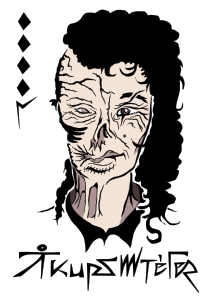
\includepdf[pages={1}]{pic_KurzWanted.pdf}
\newpage
\thispagestyle{plain}

Листовка с Друзы Вольке, изготовленная примитивным линотипом.
Надпись гласит:
<<Разыскивается живой или мёртвой Курц Штайгер.
Награда за поимку --- 70~000 лос\footnote{Лос --- валюта Друзы Вольке. 70 тысяч лос эквивалентны 305 аркан.}>>.
Лицо срисовано с портрета одного из любовников Курц --- портрет был конфискован, а его автор, Юхан Зангер, повешен за соучастие.
Позже с портрета Юхана делали ещё несколько копий для музеев и книг по истории.
% ----- PICTURE: KURZ WANTED POSTER -----

\newpage
\pagestyle{fancy}

\chapter*{Вместо предисловия}

Великий философ древности как-то говорил, что история повторяется дважды --- один раз в виде трагической пьесы, второй раз в виде клоунады.
Он жил во времена, когда люди ещё не вышли в космос, и не мог знать, что каждая история повторяется много раз --- множество мелодий с разной аранжировкой на один и тот же мотив, который затихнет лишь тогда, когда угаснет во Вселенной последняя людская цивилизация.

Осенняя война мостов, к сожалению, не исключение.
В ней отчётливо просматриваются те же нарративы, которые были вплетены в Последнюю войну на Древней Земле.
Тот же геноцид, те же жестокости, тот же страх, тот же обман, и на выходе --- всё то же сломанное, с трудом функционирующее человеческое сообщество, которое ждут десятилетия и столетия реабилитации.

Осенняя война --- первая в истории война на Тысяче Башен, в которой без всякого сомнения принимали участие демонические фракции.
Разумеется, такие войны были и до этого, но участие демонов всегда было труднодоказуемо и долгое время оставалось в поле исторических спекуляций.
Открытое появление Ада и Картеля --- признак того, насколько яростной и тяжёлой была борьба между фракциями.
Когда демоны стали называть себя демонами, когда они начали, не скрываясь, носить свои лычки и называть друг друга своими истинными именами, ценность человеческой жизни упала драматически.
Людьми играла уже не судьба, а нечто хуже --- существа, превосходящие людей по интеллекту и использующие людей как одежду.

В этой ситуации более всего вызывает интерес тот факт, что огромную роль в Осенней войне сыграл именно человек.
Человек, который прямо или косвенно спас множество людей от голода, болезней и смерти.
Человек, который прямо или косвенно повинен в смерти множества других людей.
Человек, который любил, ненавидел, обретал и терял.
Человек, которого любили, ненавидели, жалели и восхваляли.
Человек без лица, ставший лицом Осенней войны и навсегда вписавший своё имя в историю Тысячи Башен.

К сожалению, мы мало знаем про повседневную жизнь человека.
Её образ окутан легендами, большая часть которых появилась уже после её смерти.
Здесь мы приводим только свидетельства современников, безусловно достойных доверия --- людей, которые знали Курц Штайгер лично.

<<На неё было страшно смотреть.
Шрамы перетягивали её лицо, придавая ему на редкость злобное выражение.
Из глаз, носа и рта что-то сочилось, и она вытирала [лицо] платочками, для которых у неё был целый карман в куртке.
Вся её куртка была измазана в этом, потому что иногда она забывала [про платочки] и вытиралась рукавом или воротником.
Зубы у неё были, но какие-то коричневые и обломанные.
Волосы росли клочками, и она не заботилась об их чистоте.
Тело костлявое, покрытое шрамами и татуировками.
От неё постоянно шёл тяжёлый кисло-гнилостный запах --- пота, нечистот, силоса, горелого, и окружающие предпочитали держать от неё дистанцию.
Голос --- хриплый, неприятный, срывающийся.
Сложно представить более отталкивающего человека>>.

<<Когда Курц открывала рот --- все замирали.
Она говорила чисто и внятно, простым языком.
Многие закрывали глаза, чтобы её не видеть и слышать только её голос.
Она говорила о материях, в которые было сложно поверить, которые было сложно принять.
Но ей верили.
За ней шли --- десятками и сотнями, умирая в рейдах, пыточных, погибая на виселицах.
И только сама Курц неизвестно как избегала смерти в течение одиннадцати лет>>.

<<Её любили в народе.
Если проходил слух, что она появлялась где-то --- власть имущие прекращали несправедливости и начинали задабривать людей, лишь бы избежать гнева Принцессы Греллов.
Гнев был страшен --- Курц была в седле огромного полудикого козла, резвого и злого как дьявол, в её руках была рапира и сарландка [сарландская камча], вошедшая в присказку.
Такой камчой можно забить волка насмерть, а человека и подавно.
Если кто-то обижал народ, то ему говорили: погоди, Курц и тебя камчой погладит.
От неё не спасали ни стены, ни охрана, потому что никто лучше неё не лазал и не прятался>>.

<<Типичная террористка --- фанатичная и готовая на любые жертвы во имя своей цели.
Она видела что-то, что ей не по силам было принять, и сражалась с этим как одержимая.
Она говорила про существ, которые выглядят как люди, но людьми не являются.
Из-за этих существ наша земля превратилась в поле битвы, говорила она.
Я ей, конечно, не поверила поначалу, но из любопытства вступила в Сопротивление.
Жалею до сих пор.
Нет, она не соврала про тех существ, нет, мы все их видели, мы все за ними следили.
Но она очевидно закрывала глаза на их истинную силу и возможности.
Такое нельзя знать и спать спокойно.
Когда я узнала о наших врагах побольше, я прямо сказала ей, что борьба бессмысленна и она нас всех ведёт на верную гибель.
И она ответила, чтобы я убиралась прочь и не отсвечивала.
Я вынуждена была переселиться сначала на Вольке, а потом сюда [на Шампагне], потому что Охотники [на демонов] угрожали мне расправой>>.

<<Как мастер хука и глайдера Курц великолепна.
Но как человек --- редкостное говно.
С детьми она хорошо общалась, объясняла всё, но родителям их доставалось по первое число.
Если кто ребёнка [приводил] непоевшим или в одежде не по погоде, только держись.
Если локхиды или концы изношенные --- домой приходит и в дверь ломится, воняет на весь дом.
Ну а как без всего этого, семьи большие, разве за всеми уследишь?
Нервы и нервы.
Так что к ней и [детей] водили потому что выбора особо не было --- что она такая, что её мамаша придурошная>>.

<<В ней не было абсолютно ничего примечательного, кроме её уродства.
Будь у неё нос на месте, на неё никто даже бы не взглянул>>.

<<Мой отец её оперировал.
Я помню, как он вскочил среди ночи.
Десять дней была на грани жизни и смерти, но всё-таки он её вытащил.
Сказал, половину кишок из неё вытянуть пришлось.
На подарок её матери мы потом ремонт сделали в моей комнате>>.

<<Фрау Штайгер научила меня дружить со скалами и ветром.
Этого достаточно?>>

<<Мои соседи.
Шальная девчонка, осиное гнездо в одном месте.
Она рвала у меня цветы на лужайке и тискала моих кур.
Потом извинялась, а после этого я её по-новой в курятнике ловлю.
Я ей говорю: заведи уже своих, глупая, и тискай!
Она смеётся.
Пропащая душа.
Ничего плохого не скажу ни про неё, ни про родню её>>.

<<Курц была самой нежной женщиной в моей жизни.
Ни разу не обидела, не ударила, помогала всегда.
Я не жалею ни минуты о тех двух годах, что провёл вместе с ней.
Почему мы расстались?
Сложно с ней было, сложно...
Это со мной она такая была, а так вспыльчивая она, грубая в общении.
Уж на что бюргеры с Хольца [Хольцхафена] не подарок, но и они не любили её за характер.
Родичей моих и друзей против себя настроила.
Попробуйте сами быть с человеком, которого половина города готова прибить>>.

<<Курц --- достойная женщина, как и её мать.
Они обе не боялись говорить правду людям в лицо>>.

<<Она милая, но грустная.
С ней ещё ребёнком никто не хотел играть, её часто обижали.
Из-за этого она на обычную для бюргеров манеру общения реагировала очень агрессивно.
Мой отец иногда приводил её в дом, ласково говорил с ней, и она была покладистая и отзывчивая.
Потом она учила моих детей почти забесплатно>>.

<<Я не желаю о ней говорить.
Я не желаю о ней слышать.
Этого человека нет, не было и не надо в свободном городе Хольцхафен>>.

<<Когда она пропала, мы её ждали много лет, а богачей и чиновников попугивали её именем.
Ведь никто её не повесил, никто не принёс её голову.
Может, она сорвалась в пропасть.
Может, умерла от ран или своих болезней, от которых всю жизнь страдала.
Кто-то пытался выдать какой-то высохший скелет за её, да попробуй людей обмани, мы её череп видели постоянно, он у неё вместо лица.
Так или иначе, тело Курц никто не видел, и нам было этого достаточно, чтобы верить в её возвращение.
Потом прошло двадцать, тридцать лет, и я вот уже старый совсем.
Умерла, конечно.
Умерла Курц>>.

Марк Сильвия Мун, <<Осенняя война>>.
Глава 4, <<Поход Сотни>>.


\chapter{Пламя Осени}

\section{Крушение легенды}

--- Башня Дьявола рухнула!
Вставайте, вставайте!

С этих слов началось для Курц Штайгер утро, полное криков, топота и звона оружия.

Башней Дьявола издревле называли огромный кристаллический столп, росший на краю друзы Хербст.
Шли века и тысячелетия, эрозия подтачивала Башни, и они рушились одна за другой.
Некоторые падали неудачно, раздавливая целые города и деревни.
Некоторые падали удачно, на несколько сезонов превращаясь в каменный мост с одной Друзы на другую.
Чаще всего, разумеется, односторонний --- наклон и положение Башни редко позволяли одинаково хорошо идти вверх и вниз по ней.

О Башне Дьявола знали давно, к ней обращались мечты завоевателей и торговцев.
Мелкие люди, которые умирали, не дождавшись своего часа, а стареть начинали и того раньше, ждали и молили Всестроителя, чтобы Башня упала.
%{Overbuilder}
Но Башня Дьявола стояла.
По крайней мере, до сегодняшнего дня, когда её основание надломилось и исполинский кристалл встал строго горизонтально, соединив друзы Хербст и Гарда Викка.

Курц встала и протёрла глаз.
К чему вся эта беготня?
К Башне никто не подойдёт в ближайшие десять-пятнадцать дней.
Нужно время, чтобы она утряслась, плотно легла в своём каменном ложе, может быть, даже треснула напополам и отправилась в чёрную пучину Заалвира, разом похоронив все страхи и надежды людей.
%{Saalweird}
К чему эта беготня?

Курц зевнула и тут же ощутила запах свежеиспечённого куриного пирога --- с луком, картофелем и перцем.
Мама готовила его очень редко --- в последний раз это было года два назад, когда умерла её...

--- Ма-ам, --- сонно позвала Курц.
И тут же осеклась, вспомнив, что ей никто не ответит.

\section{Запах пирога}

\epigraph
{
\ml{$0$}
{Где будут павшие, там соберутся и орлы.}
{Wherever the dead shall be, there the eagles shall gather.}
}{Мф. 24:28}

Когда Курц вошла на кухню, пирог уже покинул печь и ждал на столе, сверкая подрумяненными боками.
У печи копошилась незнакомая женщина лет пятидесяти --- щуплая, седая, но ещё сохранившая гибкость и силу.
Услышав шаги Курц, женщина обернулась и нахмурила брови.

--- Садись и ешь, --- не особенно вежливо сказала она.

Курц молча повиновалась.

Традиция <<объедания>> существовала на Хербст издревле.
Всегда находились двое-трое стариков, которые освобождали молодоженов или вдовцов от необходимости готовить.
Разумеется, не бесплатно --- объедалы питались тем, что приготовили из хозяйских продуктов, а порой и утаскивали всё, что плохо лежит.
Никто не испытывал к объедалам светлых чувств, но их и не гнали --- традиция есть традиция.
Это могло продолжаться несколько дней или десятков дней после свадьбы или похорон --- всё зависело от наглости стариков или характера хозяев.

Даже в этот раз нашлась приживалка.

Курц оторвала от пирога кусочек и задумчиво нахмурилась.
Он пах очень вкусно, но было в пироге что-то незаконченное.
Обычно традиционный курник украшали каёмкой в виде подсолнечных лепестков, тестяными петушками, морковками и орешками, а также обильно смазывали маслом.
Но в этот раз корка была сухой и девственно чистой.
Это не было неуважением --- в объедании в принципе сложно искать уважение;
гостья явно нервничала и торопилась.

--- Я к тебе только на сегодня, --- сообщила незнакомка за едой, подтвердив подозрения Курц.
--- Дел по горло.

--- Если хватит сил утащить все продукты за раз, можешь даже до вечера не ждать, --- съязвила Курц.
--- Кстати, пирог очень вкусный.
Мама так точно не умела, покойная головушка.

--- Земля пухом, --- поклонилась женщина.
--- Только ты меня не позорь зазря, я не за продуктами пришла.

--- Но и не из вежливости.
Поэтому выкладывай, по возможности покороче.

Женщина разгладила юбку и вздохнула.

--- Я знала Сабину, Курц.
Достойная женщина, смелая и умная.
Про неё, конечно, разные слухи ходили в своё время --- якобы что она с контрабандистами якшается и путается с...

--- Ещё короче.

--- Ты знаешь, у меня недавно сын замуж вышел.
Такого прелестного мальчика в дом привёл, любо-дорого глядеть...

--- Что именно в словах <<ещё короче>> тебе непонятно?

Женщина поджала губы.

--- Я хочу купить у тебя дом.
Для одной тебя он чересчур велик, признай это.
Ты только убираться здесь будешь три дня.

\ml{$0$}
{--- Сложно отрицать очевидное.}
{``I wouldn't deny the obvious.}
\ml{$0$}
{Мне просто интересно, что именно тебя привело?}
{Just asking, what did exactly lead you to me?}
\ml{$0$}
{Упавшая Башня Дьявола или моя безвременно ушедшая мама?}
{The Devil Tower fallen, or my mama gone before her time?''}

--- А это моё дело, --- подбоченилась женщина.
\ml{$0$}
{--- Тревожно сейчас, облачно на горизонте, и у меня и у тебя.}
{``It's unsafe now, horizons are cloudy, both mine and yours.}
\ml{$0$}
{А я предлагаю тебе стабильную валюту в нестабильные времена.}
{All I offer you is stable currency for unstable times.}
\ml{$0$}
{Грех отказываться.}
{Too good a chance to miss.''}

\ml{$0$}
{--- Сколько?}
{``How much?''}

\ml{$0$}
{--- Сорок аркан\FM.}
{``Fourty arcanas\FM.''}
\FA{Аркана --- дорогостоящая денежная единица на Хербст, Тысяча Башен.
Представляет собой срез кристалла кварца высокой чистоты с нанесённым на него шестизначным номером.
Все арканы строго учитываются, сделки с их участием проходят исключительно под наблюдением нотариусов и баронских наблюдателей.
На арканы можно покупать только ограниченное количество товаров --- землю, недвижимость, мебель.
Курс обмена аркан на ходовую монету строго определён.
Украсть арканы невозможно, так как любые неучтённые сделки с их участием считаются недействительными.
Чаще всего арканы хранятся у нотариусов или в баронстве, так как они достаточно громоздки и неудобны для транспортировки.
Процедура подтверждения наличия определённой арканы называется арканблатт.}

--- А я твоему сыну отсосать не должна? --- спокойно осведомилась Курц.
--- И его мужу в придачу?

--- Я вошла в твоё положение, войди и ты в моё! --- вспылила женщина.
\ml{$0$}
{--- Пятьдесят --- последнее слово, не будь я Анна Аделар!}
{``Fifty is the last word of Anna Adelar, if I still am!''}

--- Вошла она, как же, --- усмехнулась Курц.
\ml{$0$}
{--- Сто аркан.}
{``A hundred arcanas.}
\ml{$0$}
{Никаких баронских кредитов, займов по соседям и долгов под честное слово, чистый скварец\FM\ из чистых рук.}
{No baron credits, no neibourhood loans, no debts under oath---clean squaretz\FM\ from clean hands.''}
\FA{Скварец --- розовый кварц, использовавшийся для изготовления аркан.}

--- Идёт, --- буркнула Анна.
--- Кстати...

\ml{$0$}
{--- Сиротские арканы\FM\ тоже не принимаю.}
{``Orphaned arkanes aren't welcome either.''}
\FA{
Сиротская аркана --- аркана, которая значится в учётных книгах, но физическое местоположение которой неизвестно.
Во время описываемых событий сиротскими являлись около 2\% аркан.
Их цена была значительно ниже, благодаря чему некоторые люди скупали их, надеясь, что аркана будет найдена и её цена возрастёт.
}

Анна хмуро кашлянула.

--- Ещё тридцать аркан платиной\FM\ за меблировку и вещи, исключая моё рабочее снаряжение и походную тележку.
\FA{Платине (платина) на Хербст --- ходовой денежный знак.
Состоит из металлической (чаще всего стальной) рамки с печатью баронства, в которую вставлен фрагмент древней печатной платы, залитый прозрачной смолой.
Каждый фрагмент уникален и выступает в роли своеобразного денежного номера.}

Гостья вздохнула и встала на ноги, замотавшись в шаль.

--- Твоя взяла, по рукам.
Ты посиди, пирог поешь, никуда не уходи.
Я плату принесу сейчас.

\ml{$0$}
{--- Я не собираюсь сидеть дома весь день.}
{``I'm not going to sit around the house all day.''}

\ml{$0$}
{--- Курц, обещаю, я за пару часиков обернусь!}
{``Kurz, I swear, I'm back in two hours!''}

\ml{$0$}
{--- Анна, перестань, --- Курц начало надоедать это ребячество.}
{``Anna, stop it,'' Kurz was getting tired of that childish game.}
\ml{$0$}
{--- Дело сделано.}
{``It's done.}
\ml{$0$}
{Я продала дом тебе и вертеться в словах не привыкла.}
{I did sell the house to you, and I'm true to my word.}
\ml{$0$}
{Не торопись, подготовь платину и бумаги, поговори с нотариусом.}
{Take your time, prepare money and papers, consult a notary.}
\ml{$0$}
{Всё равно раньше вечера я не перееду.}
{Anyway, I'm not moving until nightfall.}
\ml{$0$}
{Будет твоему сыну и его мужу семейное гнёздышко за мой счёт.}
{Your son and his husband will have their marriage nest at my expense.''}

Анна вздохнула и пододвинула пирог ближе к Курц.

--- Грубая ты женщина, Курц, --- укоризненно сказала она.
--- Сразу видно --- неименоваха.

--- Следи за словами, Анна, --- Курц задумчиво укусила пирог.
--- Ко мне ещё твои внуки придут.
Не хочу им рассказывать, как их бабка наживается на чужом горе.

Гостья негодующе фыркнула, ещё глубже замоталась в шаль и выбежала из дома, хлопнув дверью.

\section{Запах зла}

Да, для неё процесс опорожнения выглядел так --- снять мехи, выдавить содержимое, обварить кипятком, затем обработать спиртом.
Достать новые мехи, промазать уплотнителем, аккуратно вставить, привычно поморщившись от боли.
И так каждый день.

Курц знала, что от нее всегда исходит неприятный специфический запах.
Раньше её это волновало --- она натиралась маслами, пытаясь отбить вонь;
сейчас ей было всё равно.

\section{Творец}

\epigraph{Начало Творца было положено самой сутью мироздания.
Творец есть ответ на незаданный вопрос.
Но тот, кто вылепил из глины первых людей, не был равен тому, кто есть лишь ответ;
Творец сотворил себя сам --- и лишь тогда обрёл тот гений, что позволил ему стать Творцом Вселенной.}
{Хакем-Аят, 2:8--10}

Курц сняла маску, обнажив то, на месте чего должно было быть лицо.
Заросший глаз, стянутая кожа, кривое отверстие на месте рта, обнажённые носовые ходы...
Среди старых шрамов багровел ещё свежий, похожий на сколопендру.
Однажды женщине надоел не до конца закрывающийся рот, с уголка которого вечно капала слюна.
Местные врачи отказывались помогать, считая девушку безнадёжной.

--- Красивее ты от этого не станешь, --- напрямик сказала одна из них.

--- Я к тебе не за красотой пришла, идиотка, --- ответила Курц.

В конце концов она наткнулась на баронского полевого хирурга --- рассеянного, впадающего в деменцию старичка.
Тот отказался её оперировать, сославшись на трясущиеся руки, но подробно рассказал, как бы он это сделал.
Курц долго думала, примерялась, размышляла, а потом взяла бритву и исправила дефект.

Когда-то давно девчонка из Валленбергов --- местная красавица --- бросила ей в лицо:
<<Я бы лучше умерла, чем жила с этим!>>
Девчонка умерла при родах вместе с ребёнком.
Курц жива до сих пор.
И даже рот закрывается.

Дальше наступило время бриться.
Курц зачесала волосы направо, смазала висок гелем и начала брить голову.
Кипяток лишил её уха и волос на левой стороне головы;
Курц никак не могла избавиться от юношеской привычки выправлять линию волос на левом виске.

Бритва медленно сняла островки лёгкого ёжика, оставшиеся со времён болезни мамы.
Под ней оказалась уже посиневшая татуировка в виде танцующего в полёте гуся.
Шея гуся мягко обнимала заросшую глазницу, обнажённый слуховой проход был точно на месте гусиной гузки --- глупая юношеская шутка.

Мама говорила, что первый гусь в стае очень важен.
Он летит на острие клина, он самый сильный, способный разорвать воздух своей грудью и облегчить путь другим.
В полёте на глайдере эту роль выполняет проводник или первый маячок.
Перелётные птицы --- это естественные союзники мастера хука и глайдера.
Они летают от Друзы к Друзе каждый сезон, они знают воздух лучше, чем любой человек.
Многие переправы находятся там, где чаще всего пролетают гуси или лебеди.
Вторыми естественными союзниками являются козы.
Коза идёт по самому безопасному пути на скале.
Там, где идёт коза, следует сделать трассу.

Также первыми гусями называют людей, которые сталкиваются с огромными трудностями в каком-то деле, а потом делятся своим опытом с прочими.
Первым гусём можно быть в любом деле --- в ремесле, искусстве, преодолении сил природы или собственного недуга;
на Хербст существует поверье, что любой человек, которому ощутимо труднее прочих, является первым гусём --- вне зависимости от общественного положения.
Не все гуси понимают, что именно им приходится преодолевать в полёте, ведь воздух невидим и не имеет вкуса.
Но важно одно --- после каждой победы следует гоготать во всеуслышание.

Молчать о победе --- неуважение к победе.
Так гласит пословица.
Если тебе было трудно и ты справился --- это победа, не подлежащая сомнению.

\section{Тени у порога}

Едва выйдя за порог, Курц поняла торопливость Анны Аделар.
К ней уже направлялось двое человек с очевидными целями.
Справа перекатывался низенький и толстый, похожий на улыбчивый мячик, слева шёл прямой и высокий, как сосна, с идеальными резкими чертами лица и одетый по последней моде.

--- Здравствуйте, фрау Курц! --- низенький мужчина рассыпался в поклонах, оттягивая воротник на потной шее.

\ml{$0$}
{--- Уже продала, --- устало буркнула Курц.}
{``Already sold,'' Kurz wearily grumped.}

--- За сколько? --- без предисловий гаркнул второй, преградив Курц путь.

\ml{$0$}
{--- Уйди с дороги, --- процедила она, положив руку на эфес рапиры.}
{``You're on my way, man,'' she hissed with her hand on the foil hilt.}
Это было сделано очевидно для виду, но франт торопливо извинился, шагнул в сторону и отвесил короткий изящный поклон.

<<Милтон и Вагнер, владелец теплиц и маклер.
До сегодняшнего дня они едва удостаивали меня взглядом>>.

Тихо поговорив друг с другом, налетевшие орлы разочарованно исчезли в утреннем тумане.

--- Я придушу эту дрянь, --- долетел до Курц раздражённый голос Вагнера.
--- Похоже, она и правда купила дом и перепродавать не намерена.
Что Штайгеры, что Аделары --- вцепятся в дом, как клещи в задницу, и живут, пока он медленно гниёт.
\ml{$0$}
{Волчья сыть.}
{Wolf's snack.}
\ml{$0$}
{Продать за сто аркан дом, цена которому минимум двести!}
{One hundred for a house which costs at least twice that much!}
\ml{$0$}
{Старое имение --- и это даже не учитывая слухов, что там до сих пор закопан клад!}
{The Old Forwerk, and that's not counting rumours about a treasure buried there!''}

Курц ухмыльнулась.
Клад под домом Штайгеров закопан всё-таки был.
Правда, большую часть растратили ещё прошлые поколения, а последним крупным вложением, окончательно опустошившим титановую коробку, была сама Курц --- а точнее, жизнь обожжённого младенца, спасённая десятью врачами.
Сама коробка через несколько лет ушла в переплавку к жилистой, вечно чумазой и растрёпанной Катарине.
Курц никогда не видела Катарину такой счастливой --- она смотрела на огромный кусок титана так, как не смотрела даже на своего красавца-мужа в день свадьбы.

--- Титан! --- с восторгом восклицала кузничая, щупая его руками.
--- Это настоящий титан, дьявол его возьми!

--- Ты же сделаешь мне хороший хук, Катарина? --- осклабилась Сабина.

--- Бине, да я тебе даже гравировкой его украшу, с тамгой Штайгеров!

--- Катарина, ты кирша перепила?
Никакой гравировки!
Мне нужен рабочий инструмент, а не низкопробный выпендрёж для богачей!
И рапиры сделай нормальные!

Рапира являлась частью хука там, где водились пумы и барсы --- на четырёх или пяти Друзах.
На Хербст барсы давно были истреблены, но рапиру всё ещё носили --- изредка можно встретить медведей и волков, и эта встреча не несла ничего хорошего.
Вернее, медведями отговаривались, чтобы не говорить напрямую --- в горах можно встретить и зверей в человеческом обличье.

--- Хорошо-хорошо, любовь моя, --- Катарина не сводила глаз с титановой коробки.
\ml{$0$}
{--- Лучшую рапиру тебе сделаю.}
{``I'll forge you the best rapier.}
\ml{$0$}
{Две.}
{Couple.}
\ml{$0$}
{Две рапиры.}
{Couple of rapiers.''}

\ml{$0$}
{--- Если Кэцхен отдаст мне кусок коробки, я и глайдер тебе сделаю, --- с хитрым прищуром влез в разговор Уве, муж Катарины.}
{``If K\"{a}tzchen gives me a piece of the box, I'll make you a gleider on top of that,'' said Uwe, Katarina's husband.}

\ml{$0$}
{--- Так, руки с коробки убрал.}
{``Hands off the box.}
\ml{$0$}
{Мой титан.}
{My titanium.}
\ml{$0$}
{Что останется --- отдам тебе.}
{I'll give you what's left.''}

--- Ох, Бине, чувствую, разведутся они из-за этого металлолома, --- сокрушённо покачала головой Эльза, вторая жена Уве.
--- Останутся детки сиротами, с одной матерью и отцом...

\ml{$0$}
{--- Хватит называть детками моих крыс, Ойле! --- буркнула Катарина.}
{``Stop calling my rats `children', Eule!'' Katarina mumbled.}
--- Я их с собой заберу вместе с титаном.

--- А ничего, что это мои крысы, да? --- поинтересовался Уве.

Курц очень нравилось бывать у них.
В их доме всегда царил уютный бардак, совершенно неприемлемый для аккуратных и скрупулёзных жителей города.
В мастерской царил бардак совершенно другого рода, из тех, которые могут оставить без второго глаза или перерезать вены;
Курц заходить туда боялась и всегда удивлялась, как легко Уве и Катарина порхают среди этого металлического кошмара.
Уве, Катарина и Эльза замечательно друг друга уравновешивали, словно сложная система тросов на глайдере.
Но однажды Пламя Осени сожгло Уве так же, как и Сабину --- в мастерской летала вредная пыль, которая годами ослабляла лёгкие инженера.
Несколько лет вдовы жили вместе, пока не подросли дети, потом Эльза нашла себе другую семью, а Катарина так и осталась одна с кудрявыми золотыми крысами, с головой уйдя в работу.

Так было до сегодняшнего дня.
На Катарину Башня Дьявола подействовала положительно: проходя мимо её дома, Курц увидела её на веранде с мужчиной лет на десять младше.
Они мирно пили чай, не подавая никаких признаков романтики.
Но так как машинную смазку с носа и рук она стереть перед свиданием не удосужилась, лицо, шея и рубашка мужчины были в характерных чёрных полосах.
Вспомнив о смертности, людям проще выражать свои чувства.

<<Жизнь продолжается, --- весело подумала Курц.
--- Надо хоть тележку перед переездом почистить>>.

% ----- PICTURE: EAGLE ARCANA -----

\includepdf[pages={1}]{pic_EagleArcana.pdf}
\newpage
\thispagestyle{plain}

<<Счастливая>> аркана №131131, которую Анна Аделар в спешке по ошибке передала Курц в качестве оплаты за дом.

С этой арканой связано несколько городских легенд.
Одна из них гласит, что аркана была первым заработком Асканио Аделара и впоследствии оберегала семью от нищеты и несчастий.
Другая легенда утверждает, что именно после передачи Орлиной Арканы Курц семья Аделаров потеряла всех мужчин в Осенней Войне.
Третья легенда говорит, что некий Рате Абрамовитц вскоре после получения арканы унаследовал от неизвестного друга внушительную сумму денег, женился, а также нашёл врача, излечившего его жену от безнадёжной болезни.

След арканы теряется после теракта Охотников в Ротештурме --- она так и не была найдена под завалами Банка (скорее всего, украдена, увезена на другую Друзу и продана коллекционерам).
% ----- PICTURE: EAGLE ARCANA -----

\newpage
\section{Кленовое пламя}

Кленовые листья лежали на траве, словно язычки пламени.
Огнём горела и тут же сохла рябина, держа в высохших старческих руках горсти красных ягод.
И во всём этом великолепии пряталась маленькая, но прочная дверь.

Курц потянула за дверную ручку.
Дверь бесшумно открылась, и взору Курц предстала грязная мастерская, заваленная бумагой, красками, пружинами, тросами, сушёными цветами, какой-то утварью.
Посреди всего этого громоздился врачебный смотровой стол, за которым сидела маленькая сморщенная женщина и пила чай.

--- М? --- коротко осведомилась женщина.

--- Ты свободна?

--- М, --- последовал утвердительный ответ.

--- Мама умерла, --- тихо сказала Курц.

--- Ммм, --- женщина кивнула.
В её голосе прозвучало подобие сочувствия.

Курц не спеша разделась, обнажив скелетоподобный торс.
Женщина тем временем убрала со стола чашки и тарелки, накрыла замызганную поверхность чистой как снег простынёй и надела резиновые перчатки.

Спустя три часа Курц уже рассматривала в замызганном зеркале, висящем у раковины, свою новую татуировку.
Веселая кудрявая коза, застывшая в вечном прыжке.
Да, то что надо.

--- Спасибо, Мэй, --- сказала Курц и протянула женщине мешочек с платиной.

--- М, --- ответила та, забирая мешочек.

Тем временем за окном закапал дождик.

\section{Знак от Вселенной}

Однажды она любила человека.
Молодой парень с жилистым телом и горячими руками краснел и смущался.
Он очень хотел узнать, что она прячет под маской.
Она показала ему.

Спустя год, когда Курц уже уверилась в том, что её приняли, он ушёл к другой --- молодой, красивой, по выражению Курц, <<у которой жопа на правильном месте>>.
Иногда она встречала его на окраинах города --- уже начавшего седеть, полненького, лысого мужчину с пушистыми усами.
Он не испытывал особых чувств к женщине, с которой жил, но очень любил своих детей --- забавно говорил с ними и таскал их на загривке.
При встрече он смущённо улыбался и говорил <<Привет, Курц>>.
Курц кивала в ответ.

--- Не переживай, девочка, --- сказала тогда мама за обедом.
--- В тебе много способности к любви.
Я помню все твои увлечения --- ту девочку с косичками, лохматого паренька с мельницы.
А помнишь, как ты в мою напарницу влюбилась?
Тебе двенадцать было.
Вцепишься в неё и висишь, пока я тебя не стряхну.
Карлотта смеялась над тобой, как чокнутая, а ты висишь, как щеночек, и ни гу-гу.

--- И все неудачные, --- закончила Курц со вздохом.
--- Я даже в шестнадцать тайком мечтала, что я на ней женюсь, когда вырасту.
Она уже замуж вышла, дом построила, а я всё ждала, когда её сердце освободится.
А Карлотта раз --- и со скалы сорвалась.
И нету Карлотты.

Курц смахнула слезу, некстати выкатившуюся из глаза.
Мама погладила её по покрытой шрамами щеке.

--- Люди не хотели, чтобы я брала тебя на похороны Карлотты.
Особенно её родичи.
А я всё равно тебя привела, потому что знала --- ты захочешь проститься как следует.
И сказала всем этим лицемерам, что первого, кто на тебя косо посмотрит, я лично утащу за волосы и сброшу с той же скалы.

--- Такое себе счастье --- хоронить любимую.

--- Лучше, чем не хоронить.
Я на похороны своей первой любви не пошла.
Отговорилась делами, хотя на деле просто побоялась видеть его завёрнутым в красный.
До сих пор жалею.
Не проститься с близкими как следует --- всё равно что человека в мусор выкинуть...

--- Тебе всё равно везло больше.

--- Мои увлечения тоже не были удачными.
Чаще всего те, с кем я была дольше всего, не вызывали у меня никаких особых чувств.
А тех мужчин, которым я бы отдалась без остатка, не брали ни красота, ни обаяние, ни ум.

--- Как мой отец? --- хихикнула Курц.

--- Как твой отец, --- кивнула мама.
--- Я тебя забрала на память о нём.
И у тебя одно удачное увлечение всё-таки было.
Будут и другие.

--- Мне бы твой оптимизм.

--- Это не оптимизм, это признание очевидного.
Я же тебя люблю.

--- Я твоя дочь.
И, судя по всему, дочь от любимого человека.

--- Не только поэтому.
Я видела, как ты растёшь, как начинаешь ходить, как начинаешь лазать, как начинаешь летать.
Я видела, как ты преодолеваешь трудности, которых не знали другие дети.
И знаешь, я очень быстро поняла, что ты сильная и смелая, какой я никогда не была.
Ты научила меня тому, чему не научили мужчины, тысячи скал и ветров.
Я думаю, что дети нужны не только и не столько для продолжения рода, сколько для того, чтобы взрослые могли развиваться и идти дальше, когда кажется, что путь уже закончен.
Моя любовь к тебе --- гораздо большее, чем просто любовь к ребёнку.

--- Он меня не любил, видимо.

--- Любил.
Если бы не любил --- не был бы с тобой так долго.
Полюбил один --- найдутся и другие.

--- Твои-то <<другие, получше>> где задерживаются? --- пошутила Курц, брызнув на маму чаем.
Обе улыбнулись --- Сабина Штайгер никогда не страдала от недостатка поклонников.

--- С меня хватит, --- отмахнулась мама.

<<Вот и с меня тоже>>, --- сказала тогда Курц, но про себя, чтобы не огорчить маму.
С тех пор прошло пятнадцать лет, и они по-прежнему вместе.

Да и кого встретишь на крохотном островке камня, окружённом бездонной газовой пропастью?
Кого встретишь в постоянном хороводе <<работа-дом-работа>>?
Друзья юности постепенно завели семьи, умерли, улетели на другие Друзы...
Курц знала половину жителей Хербст по именам, вторую половину знала в лицо.
Она была первой, кого видели дети, покинув дома.
Она была последней, кого видели авантюристы, летящие сквозь туманную тьму в поиске счастья.

<<Я --- Штайгер.
В мир, где правят хук и глайдер, меня привела семья, которая учит детей обращаться с ними.
%{hook-en-gleider}
Разве не благородно посвятить этому делу всю жизнь, всю себя?>>

Эта нехитрая молитва помогала много лет.
Но одним промозглым дождливым днём, стоя над свежей могилой мамы, Курц поняла --- кроме неё на похороны пришёл лишь могильщик.
Никто из тех, в чьи руки Сабина Штайгер вложила хук, не нашёл времени, чтобы её проводить.

<<Мне нужны друзья>>, --- решила тогда Курц, засыпая.
Было очень непривычно не слышать дыхание мамы в другом углу комнаты.
Вселенная ответила на её призыв в своей обычной непонятной манере --- на следующее же утро рухнула Башня Дьявола.

\section{Мост}

Уже под вечер Курц тащила тележку по чистому полю к старой переправе.
Последние кварталы Хольцхафена остались далеко позади.
За прошедший день она получила столько оскорблений, сколько на её долю не выпадало за последние десять лет, и Курц была немного озадачена.

<<Вроде даже и не особо воняю, --- удивлённо думала она, обнюхивая подмышки.
--- Помылась перед уходом, одежду в порядок привела, отдохнула.
С ума посходили с этой Башней Дьявола>>.

В следующую секунду она с ужасом поняла, что в момент обнюхивания подмышки вторую подмышку тоже обнюхивали.
Снифф, снифф.
Затем кто-то осторожно ухватил её зубастой пастью за бок.

Курц заорала и схватилась за рапиру, но рапира быстро и безболезненно вылетела из её рук.
Она схватила шток, но и шток выбила зубастая пасть.
Волки повисли на её куртке, пытаясь сбить её с ног.

Курц попыталась треснуть кулаком по мокрому волчьему носу, но не могла двинуть ни рукой, ни ногой.
При этом волки метались и рычали, цепляя Курц зубами за куртку, но не причиняли ей вреда.
Когда Курц это осознала, она перестала сопротивляться.
Тут же, как по команде, волки бросились обратно под мост.
Из ниоткуда навстречу Курц вышла фигура --- красивый мужчина с лысиной и длинными золотыми кудрями, собранными сзади в хвост.

--- Кого я вижу, --- улыбнулся он кривозубой улыбкой.
--- Фрау Курц Штайгер, мастер хука и глайдера в приюте для бездомных!

--- Здравствуй, герр Рате, --- помахала Курц, кое-как поднявшись на ноги.
--- Есть место?

--- Для дочери фрау Сабины --- всегда.
Ты как?
Тебя не сильно потрепали?

--- Больше напугали.

--- Они это умеют.
Какими судьбами?

--- Я продала дом, но, похоже, прогадала, --- объяснила Курц.
Её всё ещё шатало.
--- Город наполнили беженцы, в съёмном жилье мыши пройти негде.
Меня из-за моей вони не пустили никуда, мол, <<цену сбиваю>>.

--- Денег куча, тратить не на что.
Сочувствую.
Мы люди к вони и тесноте привычные, так что милости прошу.

--- Я могу и в палатке снаружи пожить, если здесь тесно, но дьявол знает, на сколько это затянется...

--- Не оправдывайся, --- прервал её Рате.
\ml{$0$}
{--- Без дома --- значит, без дома.}
{``You have no home, that means you're homeless.}
\ml{$0$}
{Ничего зазорного в этом нет.}
{It's not a thing to shame.}
\ml{$0$}
{Проходи и не думай.}
{Come in, do not hesitate.''}

Курц кивнула и сделала шаг вперёд.
Рука Рате уперлась ей в грудь.

--- Есть ещё одно, --- вполголоса сказал он.
--- Пустить я тебя пущу в любом случае, но у меня есть настоятельная и неотложная просьба.
Здесь несколько детей, которые не могут оплатить хук.
Ни твои уроки, ни снаряжение.
В том числе и переростки.

--- Сколько переростку? --- так же тихо спросила Курц.

--- Шестнадцать.

--- Не самый безнадежный случай, --- пожала плечами Курц.
--- Ко мне приходили и в пятьдесят три.
Как я возобновлю уроки, пусть приходят.

--- Спасибо, --- коротко ответил Рате.
--- Иди вон туда, там хороший угол.
Еды у нас достаточно.
Да, кстати, не волнуйся за сохранность снаряги, тележку можешь оставить у входа.
Воры здесь есть, но у своих не воруем.
Это правило.
Вот, например, фрау Соня Сойка.

--- Привет, --- к Курц подошла низенькая девушка лет двадцати и протянула руку.
Она улыбалась криво, у неё не хватало половины зубов слева --- судя по всему, они были выбиты ударом.
Курц пожала ей руку.

--- Ой, извини, --- Сойка тут же протянула ей спрятанные в нагрудном кармане платинки.
--- Привычка.

--- Она выпендривается, --- махнул рукой Рате.
--- Как ещё может выпендриваться воровка?
Иди уже, фрау Соня, будет время пообщаться.
Фрау Курц нужен отдых и еда.

\section{Кирш}

Рядом сидел мужчина и пил кирш прямо из горла кувшина.
Он него разило спиртным и мочой.
Курц бросила на него косой взгляд.
Она недолюбливала пьяниц.

--- Не волнуйся, --- тихо сказал Рате.
--- Это герр Йон Звездочёт.
Воняет, но образованный, милый и даже пьяный ведет себя тихо.
Прям как ты.
Дебоширов тут не держим.

--- Пьяницы не контролируют себя, --- шёпотом сказал Курц.

--- Это миф, фрау Курц, миф, придуманный самими же пьяницами.
Я видел много пьяниц, и большинство из них прекрасно понимают, что делают.
Они трезвеют, если приложить им нож к горлу, они трезвеют, увидев приготовленную для них виселицу.
Если бы они действительно не могли себя контролировать, не помогло бы ничего из перечисленного.
Герр Йон --- пример пьяницы с высокой внутренней культурой.
С гигиеной только у него плоховато, но мы за ним стараемся следить.
Герр Йон, не хочешь сполоснуться и штанишки сменить?

--- К вашим услугам, --- герр Йон раскланялся, поставил кувшин и, шатаясь, пошёл к шкафам.

--- Вот, что я говорил, --- развёл руками Рате.
--- Милейший человек.

--- Кстати, о гигиене, --- вспомнила Курц.
--- Где тут постираться и помыться?

Рате указал на плещущий под мостом Химмельрот.

--- Чистейшая бесплатная вода.
Сейчас ещё и тёплая.
\ml{$0$}
{Ни в чём себе не отказывай.}
{Help yourself.''}

\section{Героин}

--- А вот там лежат три героинщика --- герр Макс Кислый Суп, фрау Айхылу Утка и фрау Анастейша Волнорез.
\ml{$0$}
{Герр Макс и фрау Айхылу местные, с Кумуштау, а фрау Стигма родом с Гарда Викки.}
{Herr Maks and frau \AE{}chylu are locals, from K\oe{}m\oe{}schtau, and frau Stigma is from Garda Wicca.}
Когда-то она была мастером хука и глайдера, как и ты, а сейчас она дожигает свою жизнь под мостом.

--- Это ужасно, --- поёжилась Курц.

--- Мы здесь никого не судим, фрау Курц.
Кстати, будешь героин?

Рате протянул женщине свёрток из фольги.

--- Нет, спасибо.

--- Это твой выбор.
Герру Максу, фрау Айхылу, фрау Стигме и герру Йону я задаю тот же вопрос каждый день, и каждый день они отвечают на него одинаково.
А вот герр Юлай отказался после пятой дозы.
И отказывается до сих пор.
Да, герр Юлай?

Худой парень в инвалидной коляске молча кивнул Курц.

--- И остальные в Ночлежке дают тот же ответ, от детей до стариков, хотя героин лежит вон там, в мешке, и все об этом знают.
Контрабандисты спихивают нам нереализованные остатки в качестве жеста доброй воли.
Если ты захочешь ширнуться, никто не скажет тебе слова.
Всестроитель не зря дал нам свободу воли, фрау Курц.
Он верил в Своих детей.
Запреты излишни и даже вредны.

Курц закатила глаза.

--- Герр Рате, при всем уважении, давай без проповедей.

--- Биркендорфа наслушалась? --- ухмыльнулся Рате.
--- Понимаю.
Он редкостный мудак.
Его проповеди читаются лишь для его собственного чёрствого сердца.
Если бы проповеди читал я...

--- ...то тебя бы линчевали в первый же день, --- закончила Сойка.

Все захохотали, даже герр Йон оторвался от кувшина, чтобы огласить Ночлежку беззубым сиплым кваканьем.

--- Не могу не согласиться, --- признал Рате.
--- Ладно.
Давай я тебя покормлю, фрау Курц, ты выглядишь голодной...

\section{Смысл}

--- Ночлежку финансируют все кто может, мы берем тех, кто в этом нуждается.
Для воров это своеобразный пенсионный фонд: если тебя не убьют в поножовщине и не повесят, то ты попадаешь сюда.
Поэтому отчисления делают многие.

--- А врачи у вас есть?

--- Блошница в городе.
Работает по тому же принципу, что и мы.

--- А где дебоширы?

--- Асоциальный элемент в Псарне.
Такая же гостиница, как и мы, только охрана посерьёзнее.
Ну и если мы защищаемся в основном от посторонних, то там, кхм, приходится защищать жильцов друг от друга.
У нас есть и детский сад --- Кладбище Выкидышей.
Мы оттуда малюток и городским пристраиваем.
Надо сказать, я им горжусь --- это не та помойная яма, которая Дом милосердия у костела.

--- Герр Рате, а какая тебе от Ночлежки выгода?

--- Отчисления, как я говорил, делают многие, и...

--- Я заглянула в вашу счётную книгу, --- перебила Курц.
--- Даже несмотря на постоянные и порой внушительные пожертвования, в конце каждого расчётного периода вы глубоко в минусе.
И тем не менее новый период начинается с кругленькой суммы.

--- Ох, убирать нам книгу надо, убирать... --- хмыкнул Рате.

--- Ты вкладываешь в Ночлежку личные сбережения.

--- Отчисления делают многие, фрау Курц!

--- Но не двадцать процентов от бюджета!

Рате смущённо развёл руками.

--- Если бы мне нужна была выгода, фрау Курц, я бы пошёл торговать героином.
А мне просто нравится работать с людьми.
Особенно с теми, которые уже не особо похожи на людей и которых никто за людей не считает.
Очень помогает понять пределы человеческой природы.
Считай это не пожертвованием, а тратой на хобби.
Богач вроде меня может позволить себе недешёвые развлечения.

\section{Волки}

--- Это действительно волки? --- Курц поёжилась.

--- Можно сказать, ручные.
Не бойся, тебя они не тронут.
Был опыт с волками, да?

--- Был, --- лаконично ответила Курц.

--- Боевые звери, --- хмыкнул Рате.
--- С ними лучше не встречаться.
Держим их как раз для этого --- периодически городская молодёжь приходит сюда выделываться.
Увидев волков, убегают почти все.
Кто не смог убежать, закопаны вон там.

Курц хихикнула.

--- Я сказал что-то смешное? --- нахмурился Рате.

--- Нет-нет, --- тут же поправилась Курц.
--- Прости.
А кто их приручил?

--- Следит за ними герр Рольф Псарь, можешь с ним поговорить, он очень много про волков знает и рассказывает интересно.
Герр Рольф!

Из угла помахал высокий, очень мускулистый мужчина с короткими светлыми волосами.
У него на переносице сидели круглые очки, которые явно были ему велики.
Он читал толстую книгу.

--- Ну и да, трогать руками их не надо и кормить тоже, могут неправильно понять.
Относись к ним как к людям из других краёв, имеющих свои суровые обычаи и правила общения.
Общается с ними только герр Рольф.
Кроме того, они опаснее обычных волков, так как натренированы давить людей поодиночке и в команде, понимают концепцию метательного и холодного оружия, на рапиру грудью не бросаются и огня не боятся.
В общем, шутить с ними категорически не советую.

\asterism

--- Сейчас я вас познакомлю, --- сказал Рольф.
--- Серый, Глаз, Рысь, \textit{сюда}.

Рольф аккуратно взял руку Курц и поднял вверх.

--- Это Курц, --- сообщил он волкам.
--- \textit{Познакомьтесь}.
Она \textit{наша}.

Волки по очереди понюхали руку Курц и вернулись на свои лежанки.

--— Ну вот и всё, совсем не больно.
Тебя теперь знают, можешь приходить сюда без страха.

--- Спасибо, --- кивнула Курц.
--- В первый раз они меня испугали.

--- Кстати, обрати внимание, в каком порядке они нюхали твою руку.
Я позвал их в том же порядке.
У волков в стае жёсткая иерархия.
Я для них просто самый сильный волк, поэтому меня слушаются.
Если я проявлю слабость --- начнётся грызня.

--- Здесь много слабых людей.
Почему волки их не трогают?

--- Вы для них --- члены стаи под моей защитой, можно сказать, ровня.
Но если вы будете их трогать руками --- возникнет вопрос иерархии, и вас могут покалечить.
С детьми проще --- волки их воспринимают как волчат и обычно мягко осаждают, чтобы те не лезли.
Кстати, раз уж зашёл разговор.
Давай я тебе расскажу, как определить иерархию в стае и отличить вожака...

\asterism

--- Тебя не смущает, что, если ты дашь слабину, тебя просто загрызут?

--- Неа, --- Рольф почесал макушку.
--- Мне нравится с ними работать.
Они как люди --- любят, ненавидят, играют, грызутся за власть, обманывают, помогают друг другу.
Идеальная модель общества.
Но они лишены человеческого обличья, из-за чего я могу смотреть на них объективно и непредвзято.
А ещё они неразговорчивы и не могут запутать меня болтовнёй, отвлекая от сути.

--- Любят?

--- Друг друга.
Людей.
Если волк интересуется тобой в свободное время, он точно в тебя влюбился.
Да, у диких зверей есть предпочтения к людям, и в отличие от людей, они не стесняются их выказывать.
Но трогать влюблённого волка все равно не стоит.
Разве что слегка и если вы наедине.

--- Наука.

--- Скорее хобби.
Волки потрясающие.
Я люблю диких зверей, но волкам и их родичам отдаю предпочтение.
\ml{$0$}
{Хотел бы ещё завести песца, тут в горах они водятся, но с этой шерстяной братией песец быстро превратится в сарландский бурек.}
{Also I'd get a snowfox, they kind lives here in the mountains, but with that wool-and-woof brethren a snowfox will be turned into a Sarland burek pretty soon.}
\ml{$0$}
{Конкуренции они не терпят.}
{They don't allow no concurrence down here.}

\section{Танцы со смертью}

Прошло несколько дней.
В Ночлежке оказалось очень душевно --- хорошая атмосфера для залечивания сердечных ран.
Периодически кто-то играл на скрипке, Рольф читал книги вслух, а герр Йон Звездочёт, когда был относительно трезв, вставлял весьма интересные комментарии.
В углу миловалась и нежно занималась сексом потрёпанная парочка --- мужчина и женщина лет сорока, неподалёку от них старушка учила внучек читать и считать.
Волки устраивали догонялки, сшибая котлы и стулья.
Беготня быстро превращалась в шуточную потасовку, которая так же быстро перерастала в серьёзную грызню, и обратно.
Границу между грызней и игрой Курц, в отличие от Рольфа, различала плохо;
видимо, даже в игре волки следовали тонким иерархическим правилам.
Иногда Рольфу приходилось встать и похлопать в ладоши, напоминая, кто здесь хозяин.
<<Будь я лет на пятнадцать моложе, мне бы эта романтика даже пришлась по душе, --- думала Курц, флегматично наблюдая за грызущимися и повизгивающими волками на фоне играющего в камушки ребёнка.
--- Но сейчас всё-таки хочется домик и цветник.
Жаль, что с этим придётся подождать, пока вся эта башенно-дьявольская шумиха не улеглась>>.

Курц чувствовала себя здесь \emph{чересчур} легко.
Она мило болтала с воровкой Сойкой, читала, привалившись спиной к герру Рольфу, помогала герру Йону менять штаны.
Ни смрад, ни странные звуки, ни неугасающий свет не могли изменить чувство, которое она испытывала.
Потом до неё дошло: она была именно там, где, по мнению чопорных бюргеров Хольца, она и должна была быть со своими увечьями.
Город людей с целыми лицами твердил ей каждый божий день, с самого детства --- <<ты хуже, ты чужая, тебе здесь не место>>.
Твердил, не говоря при этом ни слова и приветливо улыбаясь при встрече.
И только теперь, оказавшись среди маргиналов, Курц обрела молчаливое право на существование.

Героинщики Макс и Айхылу ели один раз в день, обычно вечером, обнимались и снова уходили в мир героиновых видений.
Их рёбра просвечивали сквозь кожу, они мёрзли, и им отдавали самые тёплые места у печки.
Стигма выглядела больной, но не измождённой --- для манипуляций с героином она использовала колбочки и весы, которые обеззараживала над костром, героин принимала мелкими дозами, просто чтобы не чувствовать дискомфорта, ела чаще и иногда выходила на прогулку.
У нее были пружинные часы, которые противно звенели каждые два часа.
Однажды Курц увидела её на лужайке у моста;
Стигма бегала, отжималась, подтягивалась на ветке ясеня и фехтовала палкой.
Её чёрные кудри были собраны в хвост, тёмные глаза с покрасневшими белками смотрели твёрдо и уверенно, обмётанные герпесом широкие губы были раскрыты в усилии на щербатом, покрытом сыпью лице.
Иногда она останавливалась и начинала декламировать непонятные стихи.

--- Кхм.
Можешь отойти в сторону, фрау Курц?

Курц вздрогнула и оглянулась.
Рате удобно устроился в незаметной беседке между двух дубов.
Судя по всему, он рисовал Стигму восковыми мелками.

--- Можно присесть, герр Рате?

--- Конечно.
Только говори тихо.
Если говорить громко, фрау Анастейша всегда уходит подальше.

Рате заморгал и на несколько секунд прикрыл рукой слезящиеся глаза.
Он страдал какой-то глазной болезнью, и особенно плохо ему было в ветреную и солнечную погоду, поэтому он запирался у себя в <<кабинете>>, либо прятался в кустах у входа.
Время от времени кто-то из обитателей Ночлежки --- Рольф, Сойка, Лавровый Ли, реже Юлай --- закапывали ему в глаза едкую мазь, и обычно весёлый и разговорчивый Рате весь день потом недовольно бурчал и кряхтел. % Bay Li
Поговаривали, что из-за этой болезни он и вынужден был уйти на покой --- зрение <<барона шулеров>> непрерывно ухудшалось, и лет через пять-десять он мог ослепнуть совсем.

Промокнув глаза платочком в синий горошек, Рате снова вгляделся в залитую солнцем полянку.
Восковой мелок, почти такой же тёмный, как кожа Стигмы, сделал ещё несколько штрихов.

\ml{$0$}
{--- Она ещё может выбраться, --- сказала Курц Рате.}
{``She still can get clean,'' Kurz said to Rate.}

\ml{$0$}
{--- Неа, --- покачал головой Рате.}
{``Nah,'' Rate shook his head.}
\ml{$0$}
{--- Могла бы --- выбралась.}
{``She would've if she could.}
У неё стаж больше двенадцати лет, героиновые наркоманы обычно столько не живут.
Давно бы умерла, если бы не её дисциплина и тренировки.
Но слезть она точно не сможет.
Она пыталась пару раз уменьшить --- просто уменьшить --- дозу, --- Рате болезненно сморщился.
--- Даже мне от этого зрелища было не по себе.
Больше она не пытается.
\ml{$0$}
{Так что наркоту ей не победить, но смотреть, как она борется... признай, воодушевляет.}
{So, she can't defeat her dope, but the view of her fighting ... inspires, admit it.''}

До Курц вдруг дошло.

\ml{$0$}
{--- Ты её любишь.}
{``You love her.''}

--- Я --- хозяин Ночлежки, --- с достоинством ответил Рате, отложив мелки.
--- Я отношусь ко всем жильцам одинаково.

--- Чувства невозможно контролировать полностью.
Так же как и мимику, жесты и речь.

\ml{$0$}
{--- Говори прямо, фрау Курц, что ты имеешь в виду?}
{``Speak your mind, frau Kurz, what do you mean?''}

\ml{$0$}
{--- Я была гораздо более пряма, чем ты, герр Рате.}
{``I'm more speaking my mind than you yours, herr Rate.}
\ml{$0$}
{Нет ничего плохого в том, чтобы к одному из жильцов относиться иначе, чем к остальным.}
{There's nothing wrong with treating one of your guests differently.}
\ml{$0$}
{Я думаю, люди бы это поняли, потому что это часть человеческой природы.}
{I guess most people would understand that, because it's a part of human nature.''}

--- Я никогда не заводил отношений с жильцами и не собираюсь, --- Рате скрестил руки на груди.
--- Мой авторитет держится в том числе на этом.

\ml{$0$}
{--- Если бы человек, которого я люблю, медленно умирал, я хотела бы отдать ему как можно больше любви.}
{``If the one I love was slowly dying, I'd give them as much love as I could.''}

\ml{$0$}
{--- Все мы медленно умираем, фрау Курц, с самого рождения, --- строго сказал Рате.}
{``We all are slowly dying, frau Kurz, from the very birth,'' Rate strictly said.}
\ml{$0$}
{--- Все об этом знают, и всем плевать.}
{``Everybody knows, and nobody gives a fuck.''}

\ml{$0$}
{--- Дело твоё, --- пожала плечами Курц.}
{``Suit yourself,'' Kurz shrugged.}
\ml{$0$}
{--- Мне, в общем-то, тоже плевать.}
{``As a matter of fact, I don't give a fuck either.''}

Айхылу в один день не проснулась, и её торжественно похоронили у реки.
\ml{$0$}
{Юлай плакал --- она была его подругой детства.}
{Julau were crying---she was a childhood friend of his.}
Макс Кислый Суп задумчиво ковырял землю --- видимо, понимал, кто будет следующим.
\ml{$0$}
{Бездомные пришли даже из города;}
{Stray people came even from the city;}
глядя на собравшуюся у могилы толпу, Курц ощущала щемящее чувство обиды за маму.

\textspace

Юлай каждое утро пытался сесть на инвалидную коляску.
Ему помогали, относили его к уборной.
Курц, порывшись в хламе, набила в Ночлежке несколько крючьев и блоков.

--- Вот здесь будешь садиться, --- рассказывала она Юлаю.
--- Цепляешь трос за ремень и подтягиваешься.
Не волнуйся, если поначалу будет сложно, руки со временем привыкнут и окрепнут.

--- Сразу видно, когда за дело берётся Штайгер! --- восхищённо сказал Рате, увидев крючья.

--- Идея не моя, --- пояснила Курц.
--- У бабули Коль дома было всё в тросах и блоках.

--- Это старая мастер, которая всю жизнь провела на скалах, а потом поскользнулась на ровном месте и потеряла способность ходить?

--- Она самая.
У неё была опухоль в спине.
До самой смерти потом по тросам по дому и саду перебиралась.
Пару раз чуть не расшиблась, потому что иногда любила с ветерком спуститься с крыши в сад.
Со скалами пришлось завязать, глайдером иногда занималась с напарником.

--- Потрясающая женщина! --- восхищённо сказала Сойка.

--- О да.
Крючьев не хватило немного.
Набейте потом сами ещё пару крючьев над уборной, чтобы Юлай сам мог ходить.
Метки я нанесла.

--- Сделаем, --- кивнул Рате.
--- Спасибо за идею, фрау.

\section{Типограф}

--- Ты знаешь правила, Типограф.
Ты и твой муж отлучены от Ночлежки.

--- Возьми хоть сынишку, замерзнет он на улице, --- взмолился мужчина.
--- Не могу же я его в Псарню тащить!

\ml{$0$}
{--- Ребёнка давай сюда, мы позаботимся.}
{``Give me the child, we'll look after them.}
\ml{$0$}
{А теперь вали отсюда.}
{Now, fuck off.}
Придёшь еще раз --- спущу на тебя волков.
Идём, малыш.
Как тебя зовут?

--- Альт, --- пробормотал мальчик.
\ml{$0$}
{--- Альт Шоэрманн.}
{``Alt Scheuermann.''}

--- Давай к нам, парень, --- весело сказал пузатый бородач, играющий в карты со своим таким же бородатым мужем.
--- У нас тут мужская компания, как ты привык.

--- Отлично, --- кивнул Рате.
--- Кстати, герр Хассан, герр Шолль, вы городские, поэтому напоминаю: забрать себе вы его не можете.
Только через Выкидышей.
Пока Кладбище не решит иначе, Типограф и Сколопендра --- его родители.

--- Как скажешь, герр Рате, --- кивнул второй бородач.
--- А гулять мы с ним можем?

--- Гулять можете.
Кормить можете.
Но уважайте его желания и личное пространство.

Курц смотрела вслед уходящему мужчине.

--- Что он сделал?

--- Они с партнёром напали на жильца, --- объяснил Рольф, оторвавшись от книжки.
--- Серый и Глаз отхватили им по паре пальцев, ну и от нас им досталось.
Теперь в Ночлежку им путь закрыт.

--- Бедный ребёнок, --- пробормотал Рольф.

--- Кто?

--- Альт.
Типограф и Сколопендра нашли подкидыша в куче мусора и с тех пор заботились о нём.
Все замечания Кладбища о том, что их образ жизни, мягко говоря, не подходит для воспитания, были ими проигнорированы.
Ну серьёзно, какой человек вырастет у двух закоренелых грабителей, один из которых ещё и игрок?
С другой стороны, мальчика они не обижают и отдают ему всё самое лучшее.
У него и книжки есть, он читает, даром что Типограф и Сколопендра двух букв отличить не могут.
По его словам, на него даже голос никогда не повышали, не говоря уже о насилии.
Так что формальных поводов лишить их родительских прав нет.

\ml{$0$}
{--- А почему Типограф?}
{``Why Printer?''}

--- А, он при ограблениях использовал литой шлагринг с буквами.
Он при ударе оставлял на теле непечатную надпись.
Элемент унижения для жертвы.
Потом образумился и перестал, а прозвище осталось.

--- Образумился?!

--- Представь себе.
Мальчонка этот, Альт, сказал, что это нехорошо, что грабитель должен быть благородным, как в книжке про Рольфа Каппе --- не бить жертв без надобности и вести себя вежливо.
И Типограф пообещал, что так и поступит.
Грабить, правда, не перестал, но делал это уже как порядочный грабитель, а не как отбитая мразь.
А Сколопендра благодаря Альту пару раз завязывал с фишками.
Правда, ненадолго, но обещает, что уж однажды он...
Может, если дать Альту время, он из этой парочки приличных людей сделает.
Кто знает.

--- Не многовато ответственности для ребёнка? --- буркнула Курц.

--- К сожалению, в баронстве Ротештурм нет органа, который распределяет ответственность сообразно возрасту, --- ответил Рате.
--- Приходится жить с тем, что имеем.

\section{Хартия}

--- Вон та бородатая парочка держит небольшую лавку в городе.
В основном мелкая химия --- простые лекарства, взрывчатка, чистящие средства.
Сюда приходят отдыхать.

--- Вы и таких пускаете?

--- Мы всех пускаем, фрау Курц.
Всех, кто не в чёрном списке.
Даже если сюда придет этот чёртов обдирала, Вагнер, мы обязаны его накормить и дать ему место.
Потому что Вагнер, к превеликому сожалению, не буянил в Ночлежке, да и вообще никоим образом не трогал Соседство.
Насчёт Хассана и Шолля --- любые знакомства полезны.
Они нам спихивают остатки лекарств, да и вообще безотказны, если что.
Мы таких постояльцев ценим и стараемся не наглеть --- им тоже на что-то жить надо.
Ну и, конечно, в отношении них действует Мораторий.

--- Мораторий?

--- Воры их не трогают, --- пояснила Сойка.
--- В отношении них запрещены грабёж, воровство, шантаж и рэкет.
А если трогают --- очень жалеют.

--- Хартия Моратория висит в каждой хазе, --- сказал Рольф.
--- Копия должна быть у каждого вора, если он не хочет попасть впросак.
Вот, смотри.

Курц оглядела коротенький список.
Двадцать человек.
Двадцать первым пунктом значилось: <<Курц Штайгер, мастер хука и глайдера>>.

--- До сегодняшнего дня меня не было?

--- До вчерашнего, --- поправил Рольф.
--- Всех, кто оказался без дома и пришёл за помощью, мы вписываем сразу.
Аптекарей отметили через пару вписок, когда они показали, что ведут себя прилично.

--- Странно, что нас до этого не грабили, --- задумалась Курц.
--- Мы не очень бедно жили с мамой.

--- Сабина Штайгер была в списке, --- ухмыльнулся Рате.
--- До дня её смерти.

--- Как?

--- А вот так.
Как, по-твоему, она сбывала клад в вашем доме, на который лечила свою дочь?
По законам баронства клады принадлежат баронству, за исключением небольшого процента, который даётся нашедшему и хозяину территории.
То есть, по сути, огрызки.
Мы реализовали клад через свои каналы, сохранив Сабине большую часть.

--- Эту историю знают все, --- сказал Юлай.
--- Она пришла ночью с ребёнком на руках.
До сих пор неизвестно, как она узнала о сборе --- скорее всего, выжала из кого-то из воров.
Колотила в дверь Подвала.
Когда охрана отказалась её пропускать, вытащила рапиру.
Все были в таком шоке, что пропустили её.
Пройдя на сбор, она показала ребёнка и рассказала о случившемся.

--- Она это сделала ради меня? --- Курц вдруг почувствовала, что в горле встал ком.

--- Видимо, для неё это было важно, --- сказал Рате.
--- Я бы не стал тратить такие деньжищи на полуживого младенца.
Фрау Курц, без обид.

--- Получается, вы внесли Сабину, но не внесли меня.

--- А с какой стати? --- хмыкнул Рате.
--- Фрау Сабина --- честная и смелая женщина.
А ты сосунок, из которой может вырасти что угодно.
Нет, на детей заслуги родителей у нас не распространяются.

--- А сколько вы взяли?

--- Баронство брало десяносто процентов, поэтому Соседство взяло десять.
Коринна сказала: если баронство ведет себя как вор, Соседство должно себя вести, как подобает баронству.

--- Благородно.
Жаль, что барон — не она.

--- Не обманывайся, Курц, --- Рате понизил голос.
--- Мы --- воры, и от благородства мы далеки.
Иногда бывает выбор между правильным и неправильным, и мы, как и все люди, его делаем.
Но хуже вора во власти только военный и святоша.
Потому что вор знает, что поступает плохо, а военные и клирики творят зверства полностью уверенные в своей правоте.

\section{Мужская солидарность}

--- Курт, возьми деньги, --- убеждал Типограф.

--- Нет, Виктор, --- решительно отказывался Хассан, накручивая на палец кудрявую бороду.
--- Нам с Вилли доставляло истинное удовольствие общение с Альтом.
Перестань, право, право.
У нас все дети уже разлетелись...

--- Разлетелись? --- ахнул Альт.

--- Да.
Обычно это говорят в переносном смысле, но наши с Вилли дети разлетелись буквально.
Один на Шкильдкрёте, второй на Вольке.
Так что приводи его, когда нужно, Виктор.
Нам это в радость.

--- Спасибо, Курт.
Спасибо!

--- Перестань, право.
Мужчины должны помогать друг другу в беде.
Так, Альт?

--- Мои папы так делают, они друг другу помогают!

--- Вот.
Право, почему не должны мы?

\section{Чёрный нож}

\epigraph
{Вера --- это азартная игра: хорошее развлечение, но плохой смысл жизни.}
{Надпись на надгробной плите Грегори О'Мэйли, первого Ворона Ротештурма.}

--- Пожалуйста, мама, пей! --- Курц со слезами пыталась влить в рот мамы воду.
Сабина металась в горячке, выкрикивая несвязные слова;
вода расплёскивалась, не достигая горла.

--- Злокачественный туберкулёз лёгких, --- вынес вердикт пришёдший врач.
--- Также известный как Пламя осени.
Я бы на твоём месте переночевал где-нибудь вне дома, а завтра провёл влажную уборку с отваром полыни.
Сейчас она заразна.

--- Она была совсем здорова вчера!

--- Так оно обычно и бывает, --- развёл руками врач.
--- Заболевание развивается в течение десяти-двадцати дней, иногда года, а потом человек сгорает, быстро и безвозвратно.
Судя по цвету кожных покровов, она вряд ли переживёт ночь.
Если решишь, что с неё хватит...

Врач вынул из-за пояса чёрный нож в ножнах, скреплённых сложной печатью из смолы и полосок ткани с надписями.
У Курц ёкнуло сердце.

--- Вот сюда, --- врач вытащил хирургический маркер и нарисовал на груди Сабины шестилучевую звёздочку.
--- Строго вертикально, резко, изо всей силы, проворачивать не надо.
Сломанную печать и нож принесёшь мне.

--- Можно это сделает кто-то другой? --- прошептала Курц.
В её горле стоял комок.

--- Я не могу, таков закон.
Сделать может любой человек, которому ты доверяешь, но нож и печать должна принести ты.
И не вздумай потерять печать, Курц Штайгер, иначе тебя обвинят в убийстве, ты меня поняла?

--- Поняла.
У меня нет никого, кому я могла бы это доверить.

--- В таком случае у тебя два выхода: либо дождись, пока она умрёт сама, либо возьми себя в руки и сделай то что должно.
\ml{$0$}
{Если нужно отпеть --- я могу прислать Ворона.}
{If she needs last rites, I'll send the Raben.''}

--- Не нужно, --- процедила сквозь зубы Курц.
\ml{$0$}
{--- Пусть Ворон своих птенцов отпевает.}
{``Let the Raben give last rites to his birdlings.''}

С Вороном Биркендорфом Курц связывали давние тёплые чувства.
Когда Сабина принесла пищащую обожжённую девочку на именины, Ворон отказался проводить обряд.

--- Я даже не знаю, что за зверя ты мне принесла.

\ml{$0$}
{--- Она вышла из моей утробы, --- прорычала мама.}
{``She came out of my womb,'' mama growled.}
\ml{$0$}
{--- Я, по-твоему, кто --- ящерица?}
{``Who do you think I am, a lizard?''}

\ml{$0$}
{--- Штайгер, ты слышала мой ответ.}
{``Steiger, you heard my answer.''}

\ml{$0$}
{--- У тебя имена закончились, Биркендорф?}
{``Are you out of names, Birkendorf?''}

\ml{$0$}
{--- Имён предостаточно, а вот времени на безнадёжных нет.}
{``I have plenty of names, I'm out of time for a lost cause.}
\ml{$0$}
{Она умрёт в течение десяти дней с такими ожогами.}
{She'll die in ten days with burns like those.''}

--- Чёрта с два, --- выплюнула Сабина, подхватила ребёнка и вышла из костёла.
%{``Like hell she will,'' Sabina spitted}

Именно так Курц получила своё прозвище.
По традиции Хербст, настоящее имя мог дать только Ворон, только на тридцать первом дне жизни.
Причин отказать в именинах было немного, но такое случалось.
Ходило поверье, что неименованных преследуют неприятности и ждёт ранняя смерть.
Так оно и было, впрочем --- люди заранее относились к неименованным настороженно, а порой и неприязненно.
Ведь если тебя не нарекли --- на это была причина, верно?

Как выяснилось впоследствии, Курц не только выжила, но и научилась устраивать неприятности именованным.
В детстве девочка несколько раз пробиралась в костёл и поджигала чёрную мантию Ворона.
Один раз он её за этим поймал.
Подняв за шкирку рычащее слюнявое существо, похожее на детёныша грелла\FM, он вдруг вспомнил злосчастные непрошедшие именины.
\FA{Грелл --- существо из мифологии друзы Хербст, одноглазый тролль, который смотрит в окна, выманивая людей на улицу по ночам.}

\ml{$0$}
{--- Считай, что мы квиты, Курц Штайгер, --- лаконично сказал Биркендорф.}
{``Call it even, Kurz Steiger,'' Birkendorf succinctly said.}
\ml{$0$}
{--- Ещё раз поймаю за этим --- урою.}
{``If I catch you again, you're done.''}

\section{Могила под скалой}

--- Нет, --- Курц положила нож на землю.
--- Я не могу.
Дайте лекарства.

\ml{$0$}
{--- Это не бесплатно, Курц Штайгер.}
{``It costs, Kurz Steiger.''}

\ml{$0$}
{--- Мне всё равно.}
{``It doesn't matter.}
Платина в мешке на шкафу, отсчитайте сколько нужно.

--- Вот это для того, чтобы сбить лихорадку, --- врач положил на стол баночку с таблетками.
--- А это поможет снять напряжение мышц.
Кстати, оно ослабляет дыхание, так что если вдруг ты захочешь сделать передозировку, достаточно шести...

\ml{$0$}
{--- Хватит, --- рявкнула Курц.}
{``That's enough,'' Kurz barked.}
\ml{$0$}
{--- Забирай платину, хоть всю, только проваливай.}
{``Take the platine, all the platine if you want, and piss off.''}

--- Жду тебя с ножом и печатью, --- врач вышел и аккуратно прикрыл за собой дверь.

Курц долго смотрела на черный нож.
Мама дышала тихо --- таблетки подействовали.

\ml{$0$}
{--- Давай уже, --- наконец проворчала Сабина.}
{``Hey, come on,'' Sabina finally grumped.}
\ml{$0$}
{--- Надоело притворяться спящей.}
{``I'm tired of playing sleep.''}

--- Мама! --- Курц схватила её за руку.

\ml{$0$}
{--- Всё хорошо, дочка.}
{``It's all right, Toch.}
\ml{$0$}
{Всё хорошо.}
{It's all right.''}

--- Как я без тебя? --- плакала Курц.

--- Ты справишься.
Ты справишься.
Нет, нет, доченька, маску надень и сядь.
А то я и тебя заражу...

\ml{$0$}
{--- Мне всё равно, мама.}
{``I don't care, mama.''}

\ml{$0$}
{--- Мне не всё равно, Курц.}
{``I care, Kurz.}
Кстати, я не говорила тебе, от чего умер твой отец?

Курц всхлипнула.

--- Да, я же тебе даже не говорила, что он умер, --- вздохнула Сабина.
Её лёгкие засвистели.
\ml{$0$}
{--- Я сама не могла с этим смириться.}
{``I couldn't accept that myself.}
\ml{$0$}
{Проще было сказать, что он ушёл к другой.}
{Tell that he left me for another was much much easier.}
\ml{$0$}
{Пламя Осени... --- Сабина усмехнулась.}
{The Flame of the Fall---'' Sabina laughed.}
\ml{$0$}
{--- Видать, судьба у нас с ним такая.}
{``Looks like it's our mutual fate.}
\ml{$0$}
{Одна кровь, одно сердце, одна судьба.}
{One blood, one heart, one fate.''}

Курц сидела, вытирая слёзы.

\ml{$0$}
{--- Помнишь нашу тайную скалу?}
{``Remember our secret rock?''}

--- Да.

\ml{$0$}
{--- Помнишь камень у подножия?}
{``Remember the stone at the foot?''}

--- С золотой жилой в форме прыгающего козла в скварце? --- хихикнула Курц.
\ml{$0$}
{--- Конечно, помню, мама.}
{``Of course I remember, mama.}
\ml{$0$}
{Козы --- это наше всё.}
{Goats are everything to us.}
\ml{$0$}
{Мы сами как козы с тобой...}
{You and me are like goats ourselves ...''}

--- Помнишь куст смородины у камня?
Мы ели ягоды с него.

\ml{$0$}
{--- Да.}
{``I do.}
\ml{$0$}
{Было вкусно.}
{They were delicious.''}

\ml{$0$}
{--- Похорони меня слева от камня и посади смородину на моей могиле.}
{``Bury me at the left of the stone and plant a gooseberry on my grave.}
\ml{$0$}
{Надписей не нужно.}
{No signs.}
\ml{$0$}
{Под старым кустом больно не копай, там уже занято.}
{And don't dig too deep under the old bush, it's already booked.''}

\ml{$0$}
{--- Я не смогу, мама.}
{``I can't do this, mama.}
\ml{$0$}
{Я не смогу...}
{I can't do this ...''}

\ml{$0$}
{--- Сможешь.}
{``You can.}
\ml{$0$}
{Я смогла и ты сможешь.}
{I did, and you can, too.}
\ml{$0$}
{Бери нож, Курц.}
{Take the knife, Kurz.}
\ml{$0$}
{Давай, пока я в сознании и не верчусь как рыбина на сковородке...}
{Go on, while I'm concious and not twisting like a fish in a pan ....}
\ml{$0$}
{Я люблю тебя, девочка.}
{I love you, girl.''}

Тело было завернуто в два слоя ткани --- красная парадная снаружи и плотный мешок внутри.
Цветовая кодировка --- белые для умерших своей смертью, синие для насильственной, красные двухслойные для опасных инфекций, зелёные для казнённых.
Если хоронят тело в красном, могильщики и родичи надевают маски, а гостям не разрешено подходить к могиле, они стоят поодаль.

В тот раз поодаль никого не было.
То ли стоял туман, то ли моросил дождь, было непонятно.
\ml{$0$}
{Облака пришли с севера, с Вольке.}
{Clouds came from the north, from Wolke.}
\ml{$0$}
{Золотой козёл потускнел и погрустнел.}
{The golden goat got faded and sad.}

--- Почему вы выбрали это место, фрау? --- устало спросил пожилой могильщик, поправляя сарландский бурек и обматывая шею белыми лисьими хвостами.
\ml{$0$}
{--- Здесь земля твёрже камня...}
{``The soil here is harder than a stone ...''}

\ml{$0$}
{--- Я его не выбирала, --- ответила Курц.}
{``I didn't choose it,'' Kurz answered.}
Могильщик понимающе кивнул и, вздохнув, снова взялся за кирку.

\ml{$0$}
{--- Здесь ещё одна могила, --- он кивнул в сторону куста.}
{``There's one more grave,'' he gestured toward the bush.}
\ml{$0$}
{--- Я вспомнил.}
{``I recalled.}
\ml{$0$}
{Ху.}
{Hoo.}
\ml{$0$}
{И булыжник этот красивый, и смородину.}
{That pretty boulder, those gooseberries.}
\ml{$0$}
{И такой же мешок, красный, двухслойный.}
{A bag like this, red-colored two-layered.}
\ml{$0$}
{И вопрос насчет твёрдой земли --- эх --- я уже задавал, только не вам, а одной глубоко беременной юной фрау, которую имею честь хоронить сейчас.}
{And the question about the hard soil---hoo---I already asked, not you, though, but one deeply pregnant frau I have the honour to bury right now.}
\ml{$0$}
{Ху.}
{Hoo.}
\ml{$0$}
{Фрау выглядела потрясающе --- чёрные кудри, синие глаза, полная скальная экипировка.}
{The frau was looking fantastic---black curls, deep blue eyes, full climbing equipment.}
\ml{$0$}
{Ху.}
{Hoo.}
\ml{$0$}
{На лице ни слезинки, только стылая улыбка и печаль, <<глубокая, чёрная и смертоносная, как Заалтиф>>.}
{Not a single tear on her face, only a chilly smile, and a sorrow, `deep, and black, and deadly, like Saaltief himself'.}
\ml{$0$}
{Ху.}
{Hoo.}
\ml{$0$}
{Так красиво люди выглядят только на похоронах, поверьте мне, я уж много повидал...}
{People look like this only at funerals, trust me, I've seen many things ...''}

\ml{$0$}
{--- Как звали человека, который тут похоронен?}
{``What is the name of the person buried here?''}

\ml{$0$}
{--- А вы не знаете? --- удивился могильщик, обернувшись и поправив шапку.}
{``Didn't you know?'' the gravedigger said in surprise.}
\ml{$0$}
{--- Они были неразлучны с самого детства.}
{``They were inseparable since childhood.}
\ml{$0$}
{Герберт Штайгер, родной брат вашей мамы.}
{Herbert Steiger, a sibling of your mother.''}

\section{Хольцхафен}

Хольцхафен --- чопорный городишко.
Несмотря на название, выхода к воде он не имел --- русло Химмельрота ушло за сотню километров уже лет триста как.
Вслед за Химмельротом ушла и торговля, и баронство --- дом, который Курц продала Анне Аделар, был частью бывшего баронского имения.
Единственное, чем продолжал славиться Хольцхафен --- это скалы и мастера.
Лучшей площадки для скалолазных тренировок было не найти.
Трое из семи мастеров хука на Хербст жили в Хольцхафене.

Несмотря на то, что жители Хольцхафена считались очень грубыми и чересчур прямолинейными, в практичности им отказать никто не мог --- центр торговли, как-никак.
Измерив скорость смещения русла и поняв, что за рекой им не угнаться, горожане просто разобрали порт на стройматериалы.
Фундамент, основа стен и маяк остались стоять --- не из соображений эстетики, а просто потому, что никто так и не придумал способ демонтирования сорокасантиметровых композитных стен.
Подумав и взвесив все за и против, жители Хольцхафена сделали на фундаменте порта рынок, а маяк превратили в местную достопримечательность.
Через сотню лет, когда деловая жилка из горожан испарилась, в маяке установили часы с кукушкой и факел с разноцветными вращающимися стеклами и зеркалами --- возмутительная трата средств по мнению старожилов.

\section{Дети}

\ml{$0$}
{Встреченные на улице дети делились на две категории.}
{Children in the streets fell under two categories.}
\ml{$0$}
{Первая, <<ещё не мои>>, при виде Курц убегали или прятались за родителей.}
{The first one (``not mine yet'') ran away or hid behind their parents at the sight of Kurz.}
\ml{$0$}
{Вторая, <<уже мои>>, здоровались или кивали, проходя мимо.}
{The second one (``already mine'') said hello or nodded passing by.}

--- Привет, Йозеф, привет, Эмма, --- кивала Курц в ответ.
--- Эмма, ты заменила локхиды?

--- Ещё нет, Курц, --- смущённо отвечала девочка.
--- Мастер Эрнст болеет.

--- Зайди к Катарине, у неё дороже, но и качеством повыше.
Обязательно замени локхиды, иначе я не допущу тебя к следующему занятию.
И передай своему брату, что если он будет часто пропускать --- отстанет от группы.

--- Курц, --- девочка понизила голос, --- всё так плохо с башней Дьявола?
Мы все умрём?

--- Нет, солнышко, --- Курц погладила Эмму по волосам.
--- Я не знаю, что нас ждёт, но пока у тебя в руках хук, а в волосах ветер --- с тобой всё будет в порядке.

<<Попробовала бы я сказать что-то другое.
Родители один раз уже устроили мне коллективный разнос, когда дети стали приносить домой недетские вопросы.
А всего-то о географии поговорили>>.

\section{Гонец}

Гонец стоял, сморщив кривой нос.
Курц резко захотелось сделать его нос ещё более кривым.

--- Что баронесса хочет от меня? --- осведомилась она, прочитав письмо.

--- Баронин, --- поправил её гонец.
--- В письме всё есть.

--- В письме ничего нет, --- Курц демонстративно помахала перед глазами гонца скупыми строками.

--- Значит, приезжай и уточняй, --- раздраженно ответил гонец, запахивая пальто.
--- Мне пора.

--- Что за мудак? --- поинтересовался Рате, глядя вслед уходящему.

--- Это обычный баронский служащий, --- объяснила Курц.

--- Мудак, --- поправил её Рате.

--- Да.
Обычный баронский мудак.
Ничего не поделаешь, поеду.

Курц похлопала по карманам, ища ручку.

--- Слушай, Рате...
Я помню, что тебе обещала, но уже не уверена, что смогу выполнить.

--- Всё настолько плохо?

--- Пока не знаю.
Узнаю, как вернусь.
Но на всякий случай --- сейчас напишу расписку для банка, что в случае моей смерти на задании все деньги, включая арканы, должны передать вам.
Постройте себе что-нибудь получше убежища под мостом и отправьте детей учиться.

--- Даже не знаю, что на такое сказать, --- ошеломлённо пробормотал Рате.

--- Ничего не надо, --- заверила Курц.
--- Родичей и друзей у меня в любом случае нет.
Дай мне какую-нибудь бумажку, с ними вечная проблема...

\section{Баронская дочь}

Однажды Курц довелось увидеть баронскую дочь.
Большеглазая белокожая девочка лет семи шла в сопровождении учителя и нескольких солдат.
Увидев Курц, она испуганно прижалась к учителю.
Курц было не привыкать к такой реакции, поэтому она не обратила на ребёнка особого внимания.

<<Как же давно это было, --- думала Курц.
--- Должно быть, ей сейчас около двадцати.
Ко мне её не приводили, что неудивительно --- по слухам, баронских детей хуку и глайдеру обучает заезжий мастер.
Зачем же я понадобилась баронессе сейчас?>>

\section{Выкидыш}

Служанка поклонилась.

--- Агнес, фрау.

--- Скажи, Агнес, где я могу найти баронессу... баронин Ангару?
Она посылала за мной.
Я...

--- Я знаю, кто вы, --- снова поклонилась Агнес.
\ml{$0$}
{--- Вы майстерин из Штайгеров, дочь Сабины?}
{``You're the \textit{meisterin}, Steiger kin, Sabina's daughter?}
Я вас сразу узнала, у вас, эээ... --- взгляд Агнес прыгнул на заросшую глазницу Курц и тут же испуганно отбежал в сторону, --- ...волосы как у мамы.

--- Да, меня все узнают по волосам, --- ухмыльнулась Курц.
Агнес виновато улыбнулась.
--- Можешь проводить меня к баронин?

Служанка замялась и бросила взгляд в раскрытые двери комнаты.

--- Что такое?

\ml{$0$}
{--- Фрайфрау была беременна, --- шёпотом пояснила служанка.}
{``Freifrau was pregnant,'' the servant quietly explained.}

\ml{$0$}
{--- Была? --- уточнила Курц.}
{``Was?'' Kurz asked.}

--- Была, --- грустно ответила Агнес.
\ml{$0$}
{--- Выкидыш.}
{``She lost the baby.''}

\ml{$0$}
{--- Сам по себе?}
{``Without a reason?}
\ml{$0$}
{Может, случилось чего?}
{Maybe, something's happened?''}

--- Я не знаю.
Я услышала её стон поутру, захожу --- а её перекорёжило, пена изо рта идёт и зубы скрипят...
Доктора позвала, пока доктор встала, пока прибежала --- а фрайфрау уже и плод выбросила.
\ml{$0$}
{Вся постель в крови, как будто свинью резали.}
{All sheets soaked in blood, like someone butchered a hog there.}
\ml{$0$}
{Не приведи Всестроитель...}
{O'builder forbid ...''}

Служанку передёрнуло, она поспешно потеребила радужный браслет с полумесяцем и прошептала молитву.
Курц решила сменить тему.

--- Агнес, не знаешь случайно, зачем она за мной послала?

--- Не знаю, майстерин, --- покачала головой Агнес.
--- У нас некого хуку и глайдеру учить, дети все выросли.
Меня, кстати, мама ваша учила.
До сих пор помню её <<три чечётки...

--- ...две трещотки, на глазок>>, --- усмехнулась Курц и хлопнула в ладоши.
--- Сколько скалолазов сорвалось из-за того, что они не знали это правило.
А мама умела доходчиво объяснять детям сложные вещи.
Мне бы ещё кто доходчиво объяснил, какого дьявола я здесь делаю...
В письме, в лучших традициях баронства, ни слова.

--- Вам лучше у управляющих разведать, --- улыбнулась служанка.
--- Вон туда по коридору и направо, спросите Рихарда.

\section{Шнелль}

Парень был худ, невысок.
Его можно было даже назвать красивым --- скуластое лицо, большие карие глаза, спрятавшиеся под тенью длинных чёрных бровей, тонкий нос.
И всё-таки было в нём что-то неприятное --- тонкая бородка, хитрый прищур;
таким рисовали образ дьявола.

Когда Курц вошла, незнакомец тут же ей улыбнулся.
Для Курц это было непривычной реакцией.
Его зубы торчали вперед, между передними была заметная щербинка.
Это придавало улыбке необычное очарование, и Курц поняла, что ее обладатель умело этим очарованием пользовался.
Парень улыбался, но в его размашистых бровях, острых зубах и смехе чудилось что-то звериное.
Курц уже видела такие улыбки.
Человек был очарователен ровно до того момента, пока ты не встанешь у него на пути.

Одежда незнакомца была старой, простой, но чистой и ухоженной.
Голова была коротко выстрижена, но сзади вилась тонкая косичка с вплетенными в неё лентами.
Рабочую куртку он носил, обвязав вокруг пояса, рубаха с обрезанными рукавами была ему немного велика и обнажала тощие руки и костистые ключицы.
Однако, когда парень повернулся, Курц поняла, что тонкость была обманчивой: под кожей рук очертились твердые мышцы.

--- Я ищу Рихарда.

--- Ты ищешь его там, где его нет.

--- А кого я в таком случае нашла?

--- Шнелль, --- осклабился парень.
--- Вообще я Лангзам Хетвертак, но у меня и имя неудачное, и фамилия непроизносимая.
Поэтому здесь я просто Шнелль.

--- Курц Штайгер, учитель хука и глайдера.

--- Еще одна неименованная, --- Шнелль протянул мягкую тонкую ладонь.
--- Нечасто встречаю своих.
Из-за этих ожогов?

Курц кивнула и пожала руку Шнелля, отметив, как легко он говорил о её увечьях.

--- А ты?

--- А я в безворонье родился, в Дахайме.
Старый Рольф преставился, и...

\ml{$0$}
{--- И тебе двадцать два года.}
{``And you are twenty-two.''}

\ml{$0$}
{--- Все всегда угадывают мой возраст, --- хихикнул Шнелль.}
{``Everyone would know that,'' Schnell chuckled.}

\ml{$0$}
{--- Кем ты здесь работаешь?}
{``What are you here?''}

\ml{$0$}
{--- Я гонец.}
{``I'm a messenger.}
\ml{$0$}
{Почту приношу, уношу, проверяю.}
{I bring mails, take mails, check mails.}
\ml{$0$}
{Хорошо обращаюсь с чернилами и ножом для конвертов.}
{I'm good with ink and envelope knives.''}

\ml{$0$}
{--- Может быть, ты случайно знаешь, зачем баронин Ангара меня вызвала?}
{``Maybe you know by chance, why Baronin Angara paged me?''}

\ml{$0$}
{--- Знаю, конечно.}
{``Of course I know.}
\ml{$0$}
{Профессия у меня такая --- знать.}
{That's my job, to know.}
\ml{$0$}
{Если мне не изменяет память, тебя отправляют на разведку к Тойфельстурм.}
{If I recall correctly, you're ordered to scout Teufelsturm.''}

Курц вздохнула.
Ну конечно, зачем же ещё её могли позвать.

\ml{$0$}
{--- А если память тебе изменяет? --- с надеждой спросила она.}
{``Is there any chance you recall incorrectly?'' she asked with hope.}

--- Редко она мне изменяет, Курц, --- Шнелль порылся в столе и выхватил свиток, скреплённый кучей печатей.
Затем бесцеремонно сломал печати и зачитал:
\ml{$0$}
{--- <<Курц Штайгер, мастер хука и глайдера, адрес проживания Фирте Кляйне Шпигельштрассе, дом первый>> (и единственный, как и сама Шпигельштрассе), <<бург Хольцхафен, земля Альтвассер фон Химмельрот, Друза Хербст>>.}
{``\textit{Kurz Steiger, hook-n-gleider masterin, Vierte Kleine Spiegelstraße, building one} (and only, as Spiegelstraße itself), \textit{Burg Holzhafen, Shire Altwasser von Himmelrot, Druse Herbst.}}
Ты там больше не живёшь, но всем свистеть на это.
<<Баронин Ангара Ротештурм приказывает вам, согласно Четвёртому положению, пункт один, подпункт пять, явиться в расположение баронства для получения инструкций по осуществлению разведки в области Башни Дьявола.
Разведка включает в себя следующее: оценка новообразованного Моста согласно стандартам, определённым Гильдией Хука и Глайдера>> (благополучно почившей с сотню лет как), <<а также состав и дислокацию вторженцев, пришедших со стороны Друзы Гарда Викка, согласно стандартам, определённым Военной Комендатурой Ротештурма>>.
Стандартов, естественно, никаких нет, Комендатура давно превращена в курятник повышенного удобства, но и на это всем свистеть.
\ml{$0$}
{<<Инструктаж должен быть осуществлён>>, мя-мя-мя, козьи яйца.}
{\textit{The briefing shall be}, mäh-mäh-mäh, goat's bollocks.}
\ml{$0$}
{Инструктировать тебя никто не будет, даже не надейся.}
{No one will brief you, though, no hope.}
\ml{$0$}
{Не потому что все такие вредные, а потому что никто понятия не имеет, как тебя инструктировать.}
{Not because everybody are cunts, but because no one has a clue how to do that.}
И такие приказы получили десять человек.
Двое уже в пути к Башне Дьявола, один отказался, сославшись на чирей подмышкой, и по душу ещё одного (неизвестно кого из десяти) был выслан охотник за головами, причём никто не знает, от кого именно исходил приказ о ГЛоТ, никто не знает имя охотника, и никто не знает, кто и из каких средств заплатил охотнику аванс в девятьсот платины.
Такие дела.

--- Ты сейчас пошутил насчёт охотника?

--- Неа.
Без шуток.
Убить потребовалось какого-то бандюгана, но бумаги перепутали, а потом кто-то замёл следы, чтобы скрыть ошибку.
Учитывая бюрократический бардак, удивляться не приходится.

Шнелль свернул приказ, подошёл к Курц и засунул ей в сумку.
Курц окинула парня оценивающим взглядом.

--- Ты сказал, что хорошо обращаешься с ножом для конвертов, --- припомнила она.
\ml{$0$}
{--- Ты ведь не только конверты режешь?}
{``Your knife is good not only for envelopes, isn't it?''}

Шнелль бросил на неё хитрый взгляд.

\ml{$0$}
{--- Не только.}
{``Not only.}
\ml{$0$}
{Ты хочешь взять меня с собой?}
{Do you want me to go with you?''}

--- Кто-то должен доставить мой отчёт в баронство.
\ml{$0$}
{Мне бы не помешал спутник, знающий толк в конвертах.}
{I could use a companion who knows envelopes.''}

--- Ты охотника боишься, да?

--- Естественно, я боюсь охотника!
Конечно, шанс всего лишь один из десяти, но у меня и без того высока вероятность получить пулю в задницу.

Шнелль задумался.

--- Ангара пока что в отключке, так что, думаю, я разделю с тобой прогулку.
\ml{$0$}
{Только хочу предупредить: хук --- это не моё.}
{Just a fair warning: hook is not my piece of pie.}
\ml{$0$}
{Предпочитаю равнинную местность.}
{I prefer flat terrain.''}

\section{Линейка}

--- А почему ты пошёл?

--- Ты мне интересна, --- напрямик сказал Шнелль.
--- Ты чем-то похожа на баронессу.
Та тоже гордая и за словом в карман не лезет.

--- Она не от тебя случайно беременна была? --- на всякий случай поинтересовалась Курц.

--- Нет, --- Шнелль показал зубы в ухмылке.
--- С баронессой я точно не спал.
По крайней мере, в трезвом виде.
И в слегка пьяном тоже.
Не помню такого.

--- А от кого тогда?

--- Я, по-твоему, в баронстве единственный осеменитель? --- Шнелля начала заливать краска.
--- У нас куча народу работает, многие и с детьми-подростками в имении живут.
Подружилась с каким-нибудь сыном кухарки, кто за ними уследит в таком возрасте.

--- Подружилась ли?..

--- Слушай, на что ты намекаешь?

--- Ты сам сказал, что у вас полный беспорядок.

--- \emph{Такого} беспорядка у нас нет! --- Шнелль уже был красный как рак.
--- А если и есть, то я в нём не участвовал и ничего о нём не знаю!

--- Ясно всё с тобой.
Никто никогда ничего не знает, пока пятнадцатилетняя девушка не выбросит плод и не зальёт кровью полкомнаты.

--- Обожаю этот тон.
Слышу его постоянно.
Баронесса такая: втемяшит себе что-то в голову, и не разубедишь.
И ты такая же, Курц.

--- Если что, я завязала с мужчинами, --- предупредила Курц, поймав на себе его взгляд.

--- Да я не об этом, --- поморщился Шнелль.
--- Но если уж разговор зашёл, это ты зря.
Ни к чему хорошему такое отношение не приведёт.

--- Почему?

--- Кому-то действительно никто не нужен.
Но такие люди встречаются не так часто, и ты не из них.
Для тебя потребность в партнёре --- это как потребность в еде.
Даже если тебе больно, ты всё равно ешь, верно?

--- Плохое сравнение.

--- Достаточно хорошее.
В юности у меня была одна неудача за другой, и после каждой я говорил себе <<больше никогда>>, и неудачи всё равно повторялись.

--- А почему тебя преследовали неудачи, Шнелль?

--- Да по той же причине, что и тебя.
Неименоваха не может рассчитывать на равного партнёра.
Даже будь ты красив, красноречив, трудолюбив, ты останешься неименовахой.

--- Я, если честно, списывала свои неудачи на внешность, --- призналась Курц.

--- Возможно.
Мужчины обычно менее суеверны, когда дело доходит до партнёра.
Со мной женщины если и встречались, то тайком и если других вариантов не было совсем.

--- Что изменилось сейчас?

--- В принципе ничего, --- пожал плечами Шнелль.
--- Я просто научился брать то, что мне нужно, не отвлекаясь на мелочи.

--- Ты всё ещё хочешь быть любимым.

--- Да, --- неожиданно легко согласился Шнелль.
--- Немного волнуюсь, что уже поздно.

--- Моя мама говорила, что мы не можем использовать все имеющиеся возможности.
В сутках 26 часов, но ты не можешь работать сутки.
Если хочешь чувствовать себя хорошо, тебе нужно 8 часов на сон, 2 часа на еду, час на душ и еще 3 на то, что доставляет тебе удовольствие.
То же самое с возможностями.
Лучше упустить подходящую, чем потратить силы на неподходящую.
Тебе не принесут пользы отношения, к которым ты не готов.

--- Видимо, я всё ещё чего-то жду, как и ты.

--- Мне ждать нечего.

--- Думаешь, что тебя никто не полюбит?
Тоже зря.
Судя по тому, что я про тебя слышал, ты --- одна из лучших мастеров хука и глайдера на Хербст.
Человек, который в чём-то настолько хорош, обречён быть любимым.

--- Я рада, что я взяла тебя с собой.

--- Я рад, что я согласился.

Курц спешилась и подхватила козла под уздцы.
Шнелль молча подал ей бинокль.
Курц сняла задвижку, встряхнула бинокль и подождала, пока устаканится поправка на влажность воздуха.
Утренний туман на секунду рассеялся, показав редкозубую пасть Гребня Троллей.
А вот и Линейка, Башня-ориентир, на которой сделала ровные насечки сама природа.
В руках Курц щёлкнул навигационный транспортир, взволнованно завертелась освобождённая из плена магнитная стрелка.
Три, четыре, учёт азимута, сезонный сдвиг магнитного полюса, фаза Съедобных Лун, положение Железной Луны\FM... четыре тысячи шестьсот метров до Башни Дьявола.
\FA{Тысяча Башен имеет два кольца и один связанный спутниковый комплекс, называемый Съедобными Лунами (Эсслунен, Essloonen).
Две из них видны с поверхности планеты, имеют ярко-жёлтый с синевой (<<сырный>>) цвет, третья видна только из космоса.
Этимология названия не вполне ясна, но оно в той или иной форме встречается у всех народов Тысячи Башен.
Также при навигации учитывается положение массивного астероида с мощным магнитным полем, называемого Железной Луной (Айзенлун, Eisenloon).
Железная Луна не видна с поверхности, её положение высчитывают по засечкам на кольцах.}

--- Приехали, --- сказала Курц.
--- Отсюда пойдём пешком.

Шнелль кивнул и, вытащив верёвку, начал аккуратно стреноживать козлов.

\section{Фоу-Ф}

Ложбина точно между каменным ложем и башней.
Трасса здесь была, но Башня начисто смела все засечки и ориентиры.
Вот лежит вырванный с корнем крюк, а чуть поодаль --- кусок мощёной дороги.
Больше ничего.
Курц совершенно не могла узнать знакомую местность --- опасный отрезок пути, который никак не обойти.
Если Башня внезапно качнётся, от Курц останется только горсть мясного пюре...
Ага, дерево!

Курц спрыгнула в ложбину и побежала со всех ног.
Триста метров, двести, сто...
На лету, не сбив дыхания, женщина выстрелила лёгким гарпуном в удачно попавшийся узловатый ясень, аккуратно подтянула запутавшийся в ветках трос и полезла.
И только оказавшись пятьюдесятью метрами выше ложбины, она без сил свалилась в кусты, чтобы отдышаться.

Башня Дьявола лежала крепко, как влитая.
Курц в бинокль оценила контакт на четырнадцать баллов из пятнадцати, постоянно сверяясь с истрёпанным маминым справочником.
\ml{$0$}
{Такие мосты могут стоять годами, их долговечность зависит исключительно от прочности корневого кристалла Башни и сейсмической активности региона.}
{Bridges like that can stand for years, their durability depends on solidity of the core crystall and seismic activity in the region.}
Учитывая, что Гарда Викка и Хербст были одними из самых сейсмически спокойных Друз, а прочность Башни Дьявола не вызывала никаких сомнений --- речь действительно о годах.

\ml{$0$}
{Это плохо, очень плохо.}
{It is bad, extremely bad.}
Гарда Викка не отличалась спокойствием.
Все хотели урвать кусочек плодородного берега Кровавой Чаши.
Хербст не имела прямых переправ на Гарда Викка, и это в какой-то степени помогало держаться от войн подальше.
Но теперь, благодаря Башне Дьявола, в поле сражения может превратиться и этот островок спокойствия.
Как только о мосте узнают соседние Друзы --- золотые леса будут кишеть отрядами авантюристов, идущих по направлению к Гарда Викка.

Существовала возможность взорвать мост.
Это сложно, но осуществимо.
Выдолбить несколько ниш, заложить взрывчатку и молиться, чтобы инженерия победила первобытную мощь кристалла.
\ml{$0$}
{Но тех, кому выгоден мост, чересчур много.}
{But people who can benefit from the bridge are too numerous.}
Это не только авантюристы, но и торговцы, и обычные разбойники, и мелкие правители.
Все они попытаются наложить на мост лапу как можно скорее.
И если отряды с Гарда Викка уже на Башне Дьявола, задача усложняется в разы.
\ml{$0$}
{Про Войны Мостов рассказывали всем детям, это самые кровавые страницы в истории Тысячи Башен.}
{All children are been told about Bridge Wars, it's the most bloody pages of Thousand Towers history.}
Если же враг сумеет фортифицировать подходы по эту сторону моста --- пиши пропало.

Едва Курц об этом подумала, как до неё долетели чьи-то голоса.
\ml{$0$}
{Она обратилась в слух.}
{She was all ears.}
\ml{$0$}
{Говорили двое мужчин.}
{Two men were talking.}
Их непонятная мяукающая речь перемежалась вполне знакомыми обсценными словами.
Курц ни разу в жизни не слышала звучание этого языка, но о нём слышала достаточно.

Фоу-Ф-у, язык наёмников с Гарда Викка.

Курц соскользнула в ложбину и побежала.
Она больше не думала о том, что Башня может раздавить её.
\ml{$0$}
{Надо предупредить город любой ценой.}
{The city must be warned, whatever it takes.}

\section{Налётчики}

--- А кто это у нас тут, неужели женщина? --- мужчина опустил и наклонил голову --- поза охотящегося медведя.
Курц знала, что после этого последует.

--- Ты уверен? --- засомневался второй.
\ml{$0$}
{--- Какая-то она странная.}
{``She's kinda weird.}
\ml{$0$}
{Почему лицо закрыто?}
{Why face covered?}
\ml{$0$}
{Это у них обычай такой?}
{Is it a custom here?}
\ml{$0$}
{Подай-ка голос, красавица.}
{Make some noise, you beauty.''}

Курц молча попятилась, нащупывая за спиной трёхгранную рапиру.

--- А куда это мы собрались? --- первый откровенно глумился, широко расставив руки и закрыв собой выход из пещеры.

--- Слушай, оставь её, --- поморщился второй.
--- Глаза нет, носа нет, от неё ещё и воняет как от падали.
Даже за деньги в такое не засуну...

--- Да, верно, --- первый понюхал воздух и причмокнул губами.
--- Очень жаль, фруктик с гнильцой...
Умри, навозная куча.

Движения Курц были выверены до мелочей.
Она отшатнулась, словно от неожиданности, пропустив вражеский нож слева.
Имитация неуклюжего везения, вводящая противника в заблуждение.
Затем быстрым винтовым уколом справа она проткнула врагу горло.

Налётчик взмахнул руками, словно пытаясь поймать и вернуть обратно фонтан крови, брызнувший из его шеи.
В его глазах застыло удивление.

<<На Хербст тебе не рады.
Я лишь вложила это чувство в движение клинка>>.

Второй неожиданно легко увернулся от серии выпадов.
Курц в жизни не видела, чтобы кто-то двигался с такой скоростью.
Он присел, перекатился, оттолкнулся от стены и подпрыгнул, целясь ногой в голову противницы.
Курц отклонилась... и тут же получила от висящего в воздухе мужчины удар второй ногой.

<<Обманный манёвр! --- успела подумать Курц.
--- Вот это сила...>>

В следующий миг она грохнулась спиной о камень и сползла вниз.
Рапира отскочила и исчезла где-то в темноте.
Дыхание перехватило, к горлу подступила паника, Курц не могла сделать ни малейшего вдоха.
Инстинкт выживания заставил её вскинуть руку и нажать на спусковой крючок.
Лёгкий скалолазный гарпун вошёл точно в глаз бросившегося на неё врага.
Звякнул о камень шипастый шлагринг, зажатый в жилистой руке;
опустевшее тяжёлое тело свалилось прямо на Курц, чувствительно ударив её ещё и в пах.

Вдохнуть наконец удалось.
Сначала маленькими глотками, вскоре Курц раздышалась совсем.
Но встать она не могла ещё долго, потрясённо рассматривая ещё тёплый труп человека, который едва не забрал её жизнь.

<<Их было всего двое, --- с ужасом думала она.
--- Сколько их там ещё на мосту?..>>

\section{Первый труп}

Однажды Курц уже пришлось убить человека.
Ей было пятнадцать, она цвела и пахла --- насколько вообще может цвести и пахнуть обугленный цветок.
Она провожала Карлотту до дома, надеясь на ставший традиционным поцелуй в щёчку.
Правда, Курц активно вертела головой, пытаясь превратить поцелуй в щёчку в нечто гораздо более интимное, но Карлотта строго говорила ей <<Не вертись!>> и целовала куда положено.
А потом ещё раз.
И ещё.
А потом они долго стояли обнявшись, пока не спускался муж Карлотты и не отдирал жену от настойчивой поклонницы.
Домой Курц возвращалась в лёгком опьянении и тяжёлых раздумьях.

В ту ночь им навстречу попались две женщины бандитской наружности.
Они громко хохотали, плевались и задирали прохожих.
Карлотта очень неосторожно отодвинула одну из женщин с дороги, продолжая рассказывать Курц какую-то историю.

\ml{$0$}
{--- На, ты попутала, сука бирючья?}
{``Na, lost your way, you wolfbitch?''}

\ml{$0$}
{У Карлотты в планах на вечер не значилось становиться <<сукой бирючьей>>, поэтому она вежливо извинилась и пошла дальше.}
{Karlotta hadn't scheduled being a ``wolfbitch'' for that evening, so she gently apologized and moved on.}
И тут в лопатку ей прилетел булыжник.

Начала драку Курц.
Это тёмное пятно на её совести не вытравливалось ничем.
Карлотта безуспешно попыталась перехватить спутницу, бросившуюся на обидчиц с кулаками.
Потасовка быстро перешла в поножовщину, один на одного.

Вдруг Карлотта издала крик отчаяния.
В её глазах застыл ужас.
Курц только мельком увидела её измазанные в крови руки --- и, не думая, пригвоздила вторую женщину к дереву.

\ml{$0$}
{Любовь слепа.}
{Love is a blind creature.}

--- Ребёнок, что ж ты... что ж ты делаешь... малышка моя... --- бормотала Карлотта, всхлипывая и гладя Курц по изуродованному лицу.

\ml{$0$}
{--- Нет свидетелей --- нет преступления, --- спокойно заявил ребёнок, вытирая рапиру.}
{``No witness, no crime,'' the baby calmly answered wiping her rapier.}
\ml{$0$}
{--- Нож вытащи и по земле потаскай тряпку, надо избавиться от твоих отпечатков и следов.}
{``Take out the knife and drag a rag on the ground, we should wipe out your fingerprints and footprints.''}

\ml{$0$}
{Потом были кошмары.}
{Then came nightmares.}
\ml{$0$}
{В основном шериф, тюрьма, виселица, ощущение нехватки воздуха.}
{Mostly the Scherif, a prison, a gallows, suffocation.}
\ml{$0$}
{Иногда снилась убитая --- полный ужаса взгляд умирающего, торчащая изо рта рапира, выбитые зубы...}
{Sometimes the murdered woman: a gaze, full of the fear of death, a rapier in her mouth, broken teeth ...}
Её челюсти клацали о титан, сползая по клинку, подбираясь всё ближе к руке Курц.
Курц отчаянно проворачивала клинок, заставляя кровь течь всё сильнее из открытого рта, но это не помогало.

Курц замкнулась в себе, стала меньше есть, вздрагивала от стука в дверь.
Карлотта приходила всё реже.
Наконец мама во время очередной <<болезни>> просто сказала:

--- Курц, я знаю, что у тебя на душе тяжесть, которую тебе не по силам нести.

Дальше был поток слов и слёз в тёплую мамину грудь.
\ml{$0$}
{Сабина не изменилась в лице.}
{Sabina's face hadn't changed.}
\ml{$0$}
{Может, она уже знала.}
{Maybe she already knew.}
\ml{$0$}
{А может, и нет.}
{Maybe not.}
\ml{$0$}
{Какая разница...}
{Who cares ...}

Карлотта сорвалась со скалы полгода спустя.
Причина несчастья осталась неизвестной.
Но одно Курц знала точно --- рядом с Карлоттой не оказалось Сабины Штайгер.

\section{Огнестрел}

Снаружи пещеры раздались тяжёлые шаги, и Курц притворилась мёртвой.
Сквозь полуприкрытое веко она увидела, как в пещеру нетвёрдой походкой зашёл незнакомый человек и привалился к стене, пытаясь устоять на ногах.
Вслед за ним появился Шнелль и вонзил нож незнакомцу в спину, оборвав его мучения.
Увидев Курц, он охнул и подбежал к ней.

--- Фух, ты жива, --- сказал он, вытирая пот со лба.
--- Я боялся, мне придётся докладывать Ангаре, что я ушёл в самоволку, и разведка прошла неудачно.

--- Да, всё хорошо.
\ml{$0$}
{Как у тебя погода?}
{What's the weather like out there?''}

\ml{$0$}
{--- На улице минус три, --- отрапортовал Шнелль, вытирая лезвие ножа о штаны.}
{``Minus three degrees,'' Schnell reported, wiping knife blade with his trousers.}
--- Ходят пятёрками.
Ещё одна группа скаутов прошла на юг, в сторону города.
\ml{$0$}
{Ребята очень жёсткие, лучше спрятаться, чем драться.}
{Tough guys, it's better hide than fight.}
\ml{$0$}
{Впрочем, ты и сама поняла, как я вижу...}
{However, you already got it, I see ....''}

--- Лучше бы я спряталась, --- согласилась Курц.
\ml{$0$}
{--- Можешь мне помочь?}
{``Could you help me?''}

Шнелль, крякнув, столкнул тяжёлый труп с напарницы и подобрал закатившуюся в угол рапиру.

--- Я бы на твоём месте взял нож, --- посоветовал он, рассматривая клинок.
--- Рапира --- неудачный выбор оружия в такой скалистой теснине.
Будь здесь чуть меньше свободного места, тебя бы просто убили.

--- Учту, --- Курц торопливо проверила нож у пояса.
--- Давай-ка к козлам, и побыстрее.

--- Дай мне минуту, --- Шнелль начал вытряхивать из сумки бинты и жгуты.

\ml{$0$}
{--- Шнелль, ты ранен?}
{``Schnell, are you hurt?''}

\ml{$0$}
{--- Самую малость.}
{``Just a bit.''}

\ml{$0$}
{--- Ложись, я осмотрю.}
{``Lie down, I'll take a look.''}

\ml{$0$}
{--- Курц, меня немного крутит, так что если я лягу --- я уже не встану.}
{``Kurz, I got kinda dizzy, so I lie down here, I stay down here.''}

\ml{$0$}
{--- Хватит нести чушь.}
{``Stop goatshitting.}
\ml{$0$}
{Просто подними рубаху.}
{Just lift up your shirt.''}

Курц аккуратно брызнула на рану водой из фляжки и нахмурила брови.

\ml{$0$}
{--- Это огнестрел, --- наконец выдала она.}
{``It's a gunshot wound,'' she finally said.}

\ml{$0$}
{--- Т-ты уверена?}
{``Are---are you sure?}
Мне показалось, это был пружинный самострел, и стрела срикошетила...

\ml{$0$}
{--- Он хлопнул?}
{``You heard a clap?''}

\ml{$0$}
{--- Скорее фыркнул, --- задумался Шнелль.}
{``A sniff, I'd say,'' Schnell answered.}
\ml{$0$}
{--- Вот такой маленький, размером с ладошку.}
{``Tiny like that, hand-sized.}
Улетел в расщелину, когда я этого гада порезал...

\ml{$0$}
{--- Этот <<маленький, размером с ладошку>> понаделал в тебе пять дырок одним залпом.}
{``That `tiny like that, hand-sized' stuff has made five holes in you at once.}
\ml{$0$}
{Дьявол...}
{Teufel ....''}

Глаза Шнелля расширились.
Он настойчиво скашивал глаза, пытаясь разглядеть рану.

\ml{$0$}
{--- Курц, ты же не дашь мне сдохнуть здесь, правда?}
{``Kurz, you wouldn't let me die here, would you?''}

\ml{$0$}
{--- Дыши мелкими глотками, пожалуйста, и заткнись.}
{``Take shallow breaths, please, and keep your mouth shut.}
\ml{$0$}
{Одна пулька застряла в ребре.}
{One bullet stuck in your rib.''}

\ml{$0$}
{--- Ай!}
{``Ouch!}
\ml{$0$}
{Чёрт бы тебя побрал, Курц!}
{Fuck yourself, Kurz!''}

--- Да всё уже, вытащила, --- Курц критически осмотрела окровавленный шарик.
--- Какой-то мягкий металл, точнее сказать сложно.
Он расплющился от удара о кость.
Сиди, я приведу козлов.
До баронства не поедем, попросим помощи в Хольцхафене.

Курц положила пульку в карман и выбежала из пещеры.

\section{Отравление}

\ml{$0$}
{--- Как ты себя чувствуешь?}
{``How do you feeling?}
Эй, Шнелль!

--- Живот, --- сдавленно сказал Шнелль.
Его взгляд замер, белки глаз покраснели, с уголка рта безвольно сочилась слюна.
В следующую секунду его вырвало с кровью.

\section{Через силу}

--- Дьявол, --- ругалась сквозь зубы Курц.
--- Дьявол...

Солнце уже давно зашло за Гребень Троллей, и в лесу быстро темнело.
Курц стянула со Шнелля испачканные штаны и обмыла его в озерце, аккуратно придерживая за голову.
Он был в спутанном сознании уже несколько часов.
Вода с углём помогла, но ненадолго;
на всякий случай Курц промыла и засыпала углём ещё и рану.

Ясное дело, пули были отравлены.
Когда Шнелль немного успокоился, Курц рассмотрела вытащенный ею снаряд.
Внутри оказалась полость.

\ml{$0$}
{<<Четыре пули всё ещё там>>.}
{\textit{Four bullets are still inside.}}
Курц чертовски хотелось искупаться, поесть и поспать.
Козлы тоже клевали носом.
Она наскоро прополоскала мехи с мылом в озерце --- чистые закончились, оставшиеся не было времени обработать как следует, от них смердило.
Как назло, подходили ещё и месячные, внизу живота разливалась знакомая тянущая боль.

Едва прожевав половинку бутерброда с грудинкой, Курц обмотала Шнелля одеялом, посадила безвольное тело на козла и повела упирающееся животное в темноту.

\section{Тележка}

--- Что с ним? --- Рате выбежал прямо в рубашке, без штанов.
Волки крутились рядом, обнюхивая Курц и Шнелля, но не рычали и не трогали.

--- Охохо, --- протянул Рольф, пытаясь удержать фонарь и очки на переносице.
\ml{$0$}
{--- Флопельцхен, прямой дорогой.}
{``Flohpelzchen, right that way.}
Твоя тележка пригодится.
Сейчас Сойку снаряжу тебе в помощь...
\textit{Уйди}, Рысь, не до тебя.
Блошница прямо на окраине города, доберётесь за десять минут.

--- Я даже не знаю, радоваться или нет, что ты живой вернулась, --- ухмыльнулся Рате, бросив взгляд на Курц.
--- Дружба дружбой, но сто аркан --- это сто аркан.

--- В этот раз свинья досталась не тебе, --- осклабилась в ответ Курц.
--- Желательно, чтобы она досталась Шнеллю.

Внезапно со стороны Ночлежки послышался жуткий грохот.
Все вздрогнули и оглянулись.
Герр Йон Звездочёт, качаясь, тащил тележку.

--- Герр Йон, ну куда ты лезешь, --- взмолился Рате.
--- Ты на ногах не стоишь!

--- Я хчу пмч! --- сообщил герр Йон, поблёвавая и морщась.
--- Я и нжм влдею!

--- Ножом ты сейчас себе только яйца на салат нарежешь, --- сказала Сойка.
--- Иди спи!

--- Дерьмо, --- поморщился Рате.
--- Сейчас с вами из выходных только Сойка и осталась...

--- А где эта сладкая бородатая парочка? --- спросила Сойка.

--- Хассан и Шольц в городе с ребёнком, Типограф и Сколопендра захотели увидеть сына, --- ответил Рольф, сверившись со списком.
--- Я невыходной, Курц, из-за волков.
Прости.
Герр Рате тоже.

--- Я пойду, --- в темноте показалась Стигма.
Она совершенно сливалась с ночью, белели только глаза.

--- Стигма, --- Рате нахмурился.
--- Я бы не хотел тебя отпускать.
\ml{$0$}
{Давай я уже пойду, если совсем некому.}
{Let me go, if no one else can.''}

\ml{$0$}
{--- Я, по-твоему, <<некому>>? --- осведомилась Стигма.}
{``I am, you say, `no one else'?'' Stigma coldly asked.}
\ml{$0$}
{--- Всё, хватит, Рате.}
{``Stop that shit, Rate.}
\ml{$0$}
{Я недостаточно раскисла, чтобы не выдержать небольшую прогулку.}
{I'm definitely not bad enough to fail a little walk.''}

--- Это опасная прогулка, Стигма.
Я...
Так, что за смех?

Все тут же смущённо приумолкли.

--- Герр Рате, я лезу не в своё дело, но все поймут же, --- сказал Рольф.
--- И воровские авторитеты тоже.

--- Ты лезешь не в своё дело, герр Рольф, --- резко ответил Рате.
--- И не в первый раз...

--- Он прав, герр Рате, --- поддержала Сойка.
--- Многие авторитеты женятся, выходят замуж и заводят детей.
И только ты следуешь букве закона.

--- Рате, я вернусь, --- тихо сказала Стигма.
--- Не беспокойся.

Рате хмуро кивнул.

\ml{$0$}
{--- Дозы возьми на всякий случай.}
{``Take your fix for safety.''}

\ml{$0$}
{--- Уже, --- Стигма похлопала по нагрудному карману.}
{``Already have,'' Stigma patted her breast-pocket.}
--- Сойка, грузим бедолагу на тележку.
Показывай дорогу.
Курц, я кое-что из твоего хука позаимствую...

--- Ясвми, --- булькнул герр Йон.

--- С нами, с нами, --- нетерпеливо сказала Сойка.
--- Садись в тележку.
Только раненого не придави.

\section{Сойка}

Шнелль перевернулся и застонал.

--- Заткни его! --- прошипела Сойка.
Курц аккуратно зажала Шнеллю рот полотенцем.

--- Это ещё что за морды? --- пробормотала Стигма, вглядываясь в темноту.
--- Трое мужчин, одна женщина.
Явно не местные.

--- Я знаю, кто это, --- сказала Курц.

--- А, --- в налитых кровью глазах Стигмы появилось понимание.
--- Те, с Тойфельстурма?

--- Они.
Тревогу надо поднять.

--- Тревога нам сейчас не нужна, --- сказала Сойка.
--- Подожди-ка...

Сойка прикрыла глаза.
В следующую секунду из-под её лохмотьев вылетел самострел.
Щёлк, щёлк, щёлк --- и скауты упали на мощёную улицу.

--- В городе их больше чем четверо, но курочка по зёрнышку клюёт, --- задумчиво сказала Сойка.
--- Идём, фрау.
Кто-нибудь из прохожих их сейчас обнаружит и поднимет тревогу.
Но мы уже будем далеко, и обьяснять ничего не нужно.
\ml{$0$}
{Разумно?}
{Makes sense?}
\ml{$0$}
{Разумно.}
{Makes sense.''}

--- Ты точно их убила? --- спросила Курц.

--- Значит так, одноглазая, --- Сойка резко повернулась и уткнула самострел в Курц.
--- Пока мы на деле, друг в друге не сомневаемся.
\ml{$0$}
{Я делаю всё в лучшем виде, и ты тоже.}
{I do my best, you do yours.}
\ml{$0$}
{Вопросы?}
{Any questions?}
\ml{$0$}
{Вопросов нет.}
{No questions.''}
Пошли.

--- Стой, --- Курц вдруг вспомнила.
--- Скауты ходят пятёрками, Шнелль го...

В следующий момент Сойка, уже сделавшая шаг за угол, получила мощный удар в висок и упала, словно срубленное деревце.
Стигма взревела и схватилась за рапиру.
Курц выдернула нож.

\textspace

\epigraph
{\ml{$0$}
{Птицы умирают быстро.}
{Birds die fast.}}
{Пословица Друзы Вольке, Тысяча Башен}

--- Мертва, --- Курц закрыла Сойке глаза.
--- Надо её похоронить.

--- Оставь здесь, --- Стигма указала на груду мусора.
--- Мы потом её заберём.
\ml{$0$}
{Лучше бы меня завалили, конечно...}
{It'd better be me than her, of course ...}
\ml{$0$}
{Жалко девчонку.}
{Poor child.''}

Стигма зло ударила каблуком по лицу мёртвой шпионки.
На вид погибшей было лет двенадцать.

\ml{$0$}
{--- Фоу-Ф.}
{``Foe-F.}
\ml{$0$}
{Ненавижу этих отбросов.}
{I hate that scum.}
У нас в Винокурнях их резали по подворотням.

--- Ребёнок совсем.

--- \textit{Fengri'r}.

--- Что? --- не поняла Курц.

--- \textit{Fengri'r}, --- повторила Стигма.
--- Не ребёнок.
Их с младенчества обучают в боевом братстве.
Они великолепные разведчики и психологи, умеют играть на чувствах, многие из них также хорошо владеют и оружием.
\ml{$0$}
{Но в них нет ни жалости, ни чести, потому что никто их этому не учил.}
{They haven't no mercy, no honour, for no one didn't teach 'em those things.}
\ml{$0$}
{В плен таких не берём.}
{Never don't capture them.}
Если есть подозрение, что это \textit{fengri'r} --- убиваем без разговоров.

--- Всё равно она ребёнок.

--- Где ты видела детей, которые убивают одним ударом?

Курц открыла было рот, но, подумав, промолчала.

Стигма взвесила на руке окровавленную рапиру.

--- Кстати, замечательная рапира.
Титан?

--- Да, от мамы досталась, --- кивнула Курц, прикрывая тело Сойки ветошью.

--- Сразу видно качественный хук.
Лёгкая как пёрышко.
У меня даже в голове прояснилось, как её в руки взяла.

--- А где твой хук, фрау Стигма?

Стигма промолчала и взглянула Курц прямо в глаза.
В глазах Стигмы была пустыня, и лишь слабые блики, словно Съедобные Луны, сияли над этой пустыней.
Для Курц её молчание было понятнее слов.

Герр Йон стоял настороже, оглядывая перекрёсток.
Он сжимал окровавленный нож, и в его позе и одутловатом лице не было ни унции хмеля.
Курц вдруг поняла, что видит то, чего никто не видел уже давно --- это люди, давно побеждённые химией, вдруг превратились в тех, кем когда-то были.
Но длилось это лишь мгновение.
Герр Йон опустил нож, качаясь, подошёл к тележке и грузно сел в неё.
Придавленный Шнелль снова застонал.

--- Ты знаешь дорогу в Блошницу, герр Йон?

Звездочёт сокрушённо помотал головой.

--- А ты, фрау?

--- Была там один раз, --- Стигма болезненно сморщилась.
--- Не в лучшем состоянии.

--- Не в лучшем?

--- Меня тащили, --- объяснила Стигма.
--- Там был странный поворот, как будто полукруглый с подъёмом...

--- Мы его прошли.
Вон там за углом.

--- Давай вернёмся.

--- Мы не можем медлить, фрау Стигма! --- в отчаянии сказала Курц.

--- Если я сейчас не вспомню дорогу, твой друг всё равно умрёт, --- спокойно парировала Стигма.
--- Успокойся и дай мне время.

--- ...десять скрипов колеса, поворот налево, --- закрыв глаза, считала Стигма.
--- Ещё тридцать три скрипа --- направо.
Здесь спуск.
О, а вот и он.
Курц!
Иди сюда.
Мы почти дошли.
\ml{$0$}
{Блошница вон там, внизу этой улицы.}
{Fleafur is right there, at the end of this alley.''} % Flohpelzchen

\section{Ртутная сердцевина}

--- Держи, Звездочёт, --- старик сунул в руку герра Йона бутылочку.
--- Снимет интоксикацию.

--- Да мне бы её продолжить, герр Дойхденвальд, --- грустно сказал герр Йон, разглядывая бутылочку.
--- Я что-то совсем протрезвел от этой драки, непорядок...

Вскоре к Курц вышла врач.

--- Это отравление ртутью, --- сказала женщина, снимая маску.
--- В твоей пульке были следы ртути.
К счастью, лопнула только одна пулька из пяти, и ты вытащила её почти сразу.
Если бы не ты --- участь парня была бы предрешена.

--- Могу я его увидеть?

--- Конечно.
Он уже в сознании.

Когда Курц подошла к кровати Шнелля, он тут же открыл глаза и схватил её за руку.
Курц поразилась перемене в его лице.
На нём больше не было ничего звериного, ничего дьявольского.
Шнелль смотрел на Курц, словно у его кровати неведомо как очутилась давно умершая мать.
В его глазах были удивление, непонимание и растроганность.

--- Я думал, ты меня бросишь, --- прошептал он.
Из узкого тёмного глаза вытекла слезинка и тут же высохла на горящем лице.

--- С ума сошёл, --- проворчала Курц.
--- Лежи, выздоравливай.
Потом еще зайду.

--- Мне очень жаль, что я...

--- Шнелль, без тебя я бы была уже мертва.
И Ангаре я об этом очень доходчиво написала.
Если тебя и ждёт какое-то наказание за самовольный уход в разведку, то символическое.
А живот заживёт.
Расслабься и постарайся поспать.

\section{Передоз}

--- Позаботьтесь о нём, --- Курц сунула хирургу в руку платину.

--- Туда, --- хирург показал на дверь.

--- Простите?

--- Туда, --- повторил хирург.

--- В коробку деньги клади, --- пояснил старик Дойхденвальд, сидевший у выхода.
--- Он не имеет права деньги в руки брать.
Правило такое в Блошнице.
Коробка у входа с прорезью.

--- Спасибо.
Кстати, --- Курц снова повернулась к врачу.
--- У вас нет случайно...

--- Есть, --- хирург сунул Курц жменю чистых ватных прокладок.

--- Спасибо, --- немного ошарашенно сказала Курц.
--- А как?..

--- Запах, --- пояснил хирург, указав толстым пальцем на нос, и удалился.

Когда Курц вернулась, Стигма сидела на скамеечке, привалившись к стене.
На её лбу градинами лежал пот.
Дыхание было глубоким и медленным.
Рядом лежал скомканный кусочек фольги и шприц.

<<Она вколола больше чем обычно, --- отметила Курц.
--- Посидеть с ней в больнице на всякий случай или повезти её домой?..>>

Курц пощупала нагрудный карман.
Там было пусто.
Стигма не могла уйти только с одной дозой.

<<Дьявол.
Конечно, она всё рассыпала в драке.
По темноте мы и не заметили...
Когда она поняла, её охватила паника и она промахнулась с дозой.
Ничего не поделаешь>>.

--- Вставай-ка, фрау Стигма, --- ласково сказала Курц.
Стигма нечленораздельно замычала.
--- Вставай.
Дойдём до тележки и поедем домой...

Поднимая женщину, Курц почувствовала под руками кровь.
На скамеечке остались красные полосы.

<<Я, что ли?..
Нет.
Стигма.
Как мы с тобой вовремя-то...>>

Вздохнув, Курц расстегнула Стигме ремень и начала стаскивать с неё штаны.

\section{Единственный, кто вернулся}

Ни один разведчик не вернулся.

\section{Воровская свадьба}

Курц притихла, открыв рот.
Этот обычай... он почти исчез везде, даже в костеле Вороны читали совсем другие слова.
Откуда ему взяться на воровской свадьбе?

--- Согласны ли вы быть вместе в болезни и в здравии, в раздорах и согласии, в цепях и на свободе, в бою и в минуты любви, у детской колыбели и на ступенях виселицы, пока смерть --- а случится это, судя по всему, очень скоро --- не разлучит вас?

--- Согласны, --- хором сказали Рате и Стигма.

--- Перережьте друг другу путы, --- Ясень протянули молодожёнам заточенный кусок металла.

Рате уверенно перехватил его.
Чинь --- и верёвки Стигмы упали на землю.
Чинь --- и руки Рате тоже оказались свободны.
Стигма спрятала заточку в карман и бросилась Рате в объятия.
Все засвистели и ликующе закричали.

<<Она улыбается, --- ошеломлённо думала Курц.
--- Я ни разу не видела, чтобы Стигма улыбалась>>.

Рате целовал её в лоб раз за разом.
По его щекам текли слёзы.
Стигма, зажмурившись, гладила его шею.

--- Можете поцеловаться в губы, если хотите, --- намекнули Ясень.

--- Не хотим, --- хором ответили Рате и Стигма.

Ясень развели руками и сошли с венчального пня.

--- Празднуйте тогда, прощелыги, --- обратились они к толпе.
Все снова ликующе закричали.

\asterism

--- Я уж думали, ты никогда на ней не женишься, --- ухмыльнулись Ясень.

--- Я не ожидал такой реакции, --- признался Рате.
--- Тем более от тебя.

--- Я рады за тебя, герр Рате, как и все твои жильцы.
А закон...
Законы писаны людьми и для людей, и только людям решать, когда им следовать, а когда нет.
В конце концов, с какой стати воры должны всегда чтить закон, даже воровской?

--- Ну ты это, поосторожнее, --- нахмурился Рате.

--- Это между нами, конечно же, --- Ясень похлопали Рате по плечу, осушил кружку и встал.
--- А теперь извиняюсь, мне срочно надо отлить.

\asterism

--- Шериф, --- буркнул Рате.
--- Ожидаемо.

--- Зашёл на огонёк, --- сообщил шериф.
--- Что такое, герр Рате?
Хербст на пороге войны, а вы празднуете.

--- При всем уважении, шериф, Хербст уже в состоянии войны, --- сказала Курц.

--- От меня требуют действий, герр Рате, --- продолжил шериф, пропустив слова Курц мимо ушей.

--- Разумеется, --- кивнул Рате.
--- Только я не вполне понимаю, при чем здесь моя свадьба.

--- О, так это ваша свадьба?
Долгих лет.
Тяжёлые нынче времена, герр Рате.
Хербст, как я уже сказал, на пороге войны.
Хотим мы мародерства?
Нет.
Хотим мы всплеска криминала?
Нет.
Поэтому, именем закона, который я представляю, я вам сообщаю --- в отношении всех преступлений вступает в силу закон военного времени.

Гости затихли и переглянулись.

--- Кто вас уполномочил сделать такое заявление, шериф? --- осведомилась Курц.
--- Из баронства не было ни слова о введении подобных мер.

--- Ротештурм далеко, Курц Штайгер, и по большому счёту на Хольцхафен баронству плевать.
Власть здесь я.

--- Шериф, --- раздался сзади тихий голос.

--- Я ещё не закончил, так что...
Эээ, здравствуйте, франн Коль.

--- И тебе не хворать, шериф, --- сказали Ясень, кладя шерифу руку на плечо.
--- Если хочешь делать заявления --- делай их Соседству и не порти людям праздник.
Что такое, в самом деле.
Ты первый день на посту?
Твоя семья не обучила тебя манерам?

--- Я уполномочен...

--- Мы тебя уже поняли, --- оборвали его Ясень.

Помощники шерифа подняли пистолеты и рапиры.
Волки вскочили с лежанок и зарычали.

--- Серый, Глаз, Рысь, \textit{стоять}, --- тут же бросил Рольф, снимая очки и поднимаясь с кресла.
--- \textit{Сто-ять}.
\textit{Ждать}.

Шериф оглядел собравшихся гостей.
Они уже успели похватать ножи, заточки, вилки, вюргехольц, шлагринги и вообще всё, что было поблизости и подходило для боя.
Быстро оценив соотношение сил, шериф кивнул.

--- Если франн Коль так желает, я сделаю заявление Соседству.

Затем повернулся к Рате и Стигме:

--- Долгих лет, герр, фрау.
Прошу меня простить за вторжение.
Ещё увидимся.

--- Вот и закончился наш медовый месяц, фрау Стигма, --- грустно сказал Рате.
--- Закончился, не успев начаться.

Стигма молча прижалась к его плечу и прикрыла глаза.

\asterism

--- Ничего нового, --- пробормотал Рате.
--- Шериф всегда для подобных выкрутасов выбирает самую уязвимую часть воровского сообщества.
В этот раз он выбрал Ночлежку.

--- На Кладбище у него ума хватило не соваться, --- присовокупили Ясень.
--- Прошлый шериф очень любил навещать Выкидышей с внезапными проверками и не вполне ясными целями, и мы прирезали троих его помощников прямо у здания суда.
\ml{$0$}
{С соответствующей пояснительной запиской.}
{With the relevant explanatory note.}
Новый шериф и его кодла урок усвоили.

\asterism

--- Я хотела сделать тебе подарок.

--- Ты не обязана...

--- Я и не сказала, что я обязана.
Для меня будет честью, если ты это примешь.

Курц положила на стол штоки.

--- Титан лёгкий, так что я ещё и запаску таскаю, --- пояснила она.
--- Но она мне не понадобилась ни разу.
Тебе нужнее.
Ну и это...

Курц протянула Стигме рапиру.

--- Она тебе понравилась.

Стигма осторожно подняла рапиру.

--- Я не могу это принять.

--- Пожалуйста, --- Курц сжала смуглую руку Стигмы.

--- Я не смогу, Курц.
Моё тело уже не служит мне как раньше.

--- Начинай с малого.
Будь осторожна.
Обучай своё тело заново, как ребёнка.
Я знаю, что ты хочешь вернуться на скалы.
Я бы хотела.
В конце концов, это всего лишь героин.

Стигма заулыбалась и потёрла бритую голову.

--- Ты сама рада свадьбе?

--- Я была против, --- сказала Стигма.
--- Не хочу быть для него обузой.

--- Обуза --- это человек, который покорился своей судьбе.
Насколько я тебя знаю, ты не будешь обузой.

--- Я покорилась судьбе в тот момент, когда вколола первую дозу.

--- А я --- когда меня ошпарило кипятком в возрасте нескольких дней.

Стигма кивнула, показывая, что она поняла намёк.

--- Я думаю, ты рада.

--- Не знаю.
Чувств как таковых у меня давно уже не было.
Есть что-то, но чувствами в привычном понимании это сложно назвать.
На самом деле, я устала и с удовольствием бы прилегла.

Стигма бессознательно пощупала нагрудный карман.

--- Тебе помочь?

--- Нет-нет, я сама, --- рассеянно сказала невеста.

--- Я с тобой, фрау Стигма, --- Рате тут же встал.
--- Уложу тебя хотя бы.
И пятнышки твои надо мазью помазать...

Уголки широких чёрных губ Стигмы чуть-чуть приподнялись.

<<Чувств нету, ага, --- хмыкнула про себя Курц, глядя им вслед.
--- Что у одного, что у другой.
Загнали свои чувства, как гвоздь в стену --- только шляпки торчат>>.

\chapter{Схизма}

\section{Поклон}

Курц прошла в костел.
По правилам, ей следовало склонить голову, но она этому правилу никогда не следовала.

--- Никакого почтения! --- укоризненно зашептали старухи.

--- Пусть Всестроитель отдаст мне моё имя, и я отдам им поклон, --- эта фраза стала для Курц традиционной.

Внутри шла проповедь, но за кафедрой стоял не Биркендорф, а какая-то молодая женщина.
На вид лет двадцать пять, не больше.
Воронское одеяние было ей чересчур велико в плечах, она сутулилась, но из её уст текла уверенная, поставленная речь клирика:

--- ...Чему нас учит эта история, правоверные?
Всестроитель (мир им!) лишены предпочтений.
Они никому не оказывали и не окажет милости рассказать Свою волю и Свои планы.

Курц прислушалась.
Это что-то новенькое.

--- Никому и никогда, --- продолжала воронин, --- не дозволено будет узнать, судимы ли мы будем или вознаграждены, кроме как по прошествии земной жизни.
Но если живому человеку не суждено узнать мерила и веса, по которым будут взвешивать его поступки, то суд несправедлив и вознаграждение незаслуженно, а Всестроитель (мир им!) не может быть несправедливы.
Блудные ли мы дети или отправлены в путешествие по Их воле, мы будем приняты в Их лоно вновь, без осуждения и без наград.

Курц сама не заметила, как её рот открылся.
Клирик нарушает основы вероучения, по факту ни в чём им не противореча!

--- Мы не можем ссылаться на Всестроителя (мир им!) как на судью в человеческих делах.
Судьями в делах человеческих людям и быть.
Гнев старших, осуждение современников, стыд потомков --- единственный суд, который у нас есть.

\asterism

--- Пошла вон отсюда!

Крик Биркендорфа окатил Курц как ледяной дождь, едва она успела открыть дверь.
Воронин вышла спокойно, с гордо поднятой головой.
На её лице замерло выражение выполненного долга.

--- Всестроитель (мир им!), --- выдохнул Биркендорф.
--- Эти схизматики добрались и сюда.
Салавата сотворить не успел, как она за кафедрой оказалась...
Чего тебе нужно, Штайгер?
Снова пришла у Всестроителя (мир им!) требовать имя?

--- Справедливости ради, в имени отказал мне ты, а не Всестроитель, --- огрызнулась Курц.
--- <<Судьям в делах человеческих людям и быть>>.

--- Безликая, прости меня Всестроитель (мир им!), --- Биркендорф потеребил радужный браслет.
--- Заканчивай с этой ересью и говори, зачем пришла.

Курц прикрыла дверь.

--- Дело есть.

\asterism

--- В общем, если вкратце, мне нужна твоя способность дурить людям головы.

--- Ты умудрилась в одно предложение оскорбить меня, мою веру и попросить у меня помощи, --- хмыкнул Биркендорф.
--- Ты владеешь словом не хуже чем хуком.
Не вполне понимаю, зачем тебе нужен я.

--- Фоу-Ф уже у ворот Хольцхафена.
Шериф вознамерился устроить здесь военную диктатуру.
Ему противостоит Соседство, но, учитывая ситуацию, не очень эффективно.
Баронство и городской совет самоустранились, голоса гильдий не слышны, потому что им прямо заявили, что в военное время их мнение ничего не значит.
Нужен противовес военным.
Мирное население в опасности.

--- Кто именно?

--- Ночлежка.

--- Воровской приют под Зангербрюкке?
Кажется, им владеет бывший <<Барон шулеров>>, Рате Абрамовитц.

--- Да, это так.

--- Я слышал, что шериф намеревается зачистить мост.

--- Что?!

--- А, так ты не поэтому сюда пришла, --- Биркендорф потёр нос.
--- Ладно, мой грех, сболтнул.
Да, шериф действительно собирается зачистить воровские притоны под интересными предлогами.
Предлоги мне неизвестны, не спрашивай меня.
О Всестроитель (мир им!), сколько же мне теперь свой длинный язык замаливать...

--- Не надо ничего замаливать, я бы и так об этом узнала.
Просто защити Ночлежку.
Это бездомные, Гектор, старики, дети и немощные.
Твоя паства.
Они не представляют опасности, и им некуда больше идти.

--- Я тебя понял, Штайгер.
Ночлежка.
Кто-то ещё?

--- Этого недостаточно, святоша?

--- Я подумал, что ты захочешь, чтобы я позаботился и о Кладбище Выкидышей, и о Блошнице.
У меня много разных прихожан, Штайгер, и тайну исповеди я поклялся блюсти до смерти.
Есть ещё Псарня, кажется.
Так?

Курц невольно почувствовала себя пристыженной и кивнула.

--- Да.
Они тоже нуждаются в защите.

Биркендорф задумался.

--- Гектор, я тебя знаю как облупленного, --- проникновенно сказала Курц.
--- Ты тот ещё мудак, но ты не милитарист и не будешь поддерживать шерифа.

Ворон встал и подошёл к зеркалу.
Его одежды зашуршали.

--- До последнего не хотел ввязываться в эту историю.
Не думал, что Посланец примет твой облик.

--- Так ты согласен?

--- Не ради тебя, Штайгер.

--- Я не настолько самонадеянна, --- ухмыльнулась Курц.
--- Тебе нужна помощь?

--- Разберусь, --- Биркендорф махнул рукой, показывая, что разговор закончен.
--- И ещё у меня просьба, Штайгер: не приходи больше в костёл.
Никогда.
Запретить я тебе не могу, поэтому прошу по-человечески --- сюда ни ногой.

\section{Удар в спину}

--- Этот \textit{фотценлеккер} привёл сюда ополчение, --- процедил Рате.

--- Доброго вечерочка, герр Рате, --- шериф даже не пытался скрыть злорадство человека, отыгрывающегося за перенесённое унижение.

--- В чём дело, шериф? --- сурово сказал Рате.
--- Это приют.

--- Приют, который не значится в кадастровых списках, --- поправил шериф.
--- Герр Рате, как я уже говорит, жители не хотят разгула преступности.

--- Так идите к Соседству.
При чём здесь мы?

--- Действительно, --- шериф почесал щёку.
--- Я обязательно к ним зайду.
Но сначала я хочу донести до вас, что мост, под которым вы столь уютно расположились, имеет стратегическое значение.
И потому я прошу вас освободить Зангербрюкке в ближайшие сутки.

Воцарилось молчание.

--- Этим людям некуда идти, шериф, --- тихо сказал Рате.

--- Друза Хербст огромна.
Они могут идти куда хотят.
А свободный город Хольцхафен разместит здесь силы, чтобы отразить неприятельский удар.

--- Давно он стал свободным, шериф? --- поинтересовалась Курц.

--- Он всегда был свободным, фрау Курц.
Баронство когда-то...

--- Баронство когда-то располагалось в доме, в котором моя мама меняла мне пелёнки, --- перебила Курц.
--- Эту историю можете приберечь для туристов.
Мне интересно --- вы серьёзно собрались в столь тяжёлые времена требовать автономию от Ротештурма?

--- Баронство прямым текстом отказало нам в военной помощи.
Это значит...

--- Это значит, что надо окончательно испортить отношения, объявив о своем суверенитете?

--- Если баронство не может нас защитить, в чём его смысл?

--- А вы можете?

--- Я уже вас защищаю.

--- От чего вы нас защищаете, шериф? --- раздался со стороны звучный голос.
--- От приюта для бездомных?

Шериф оглянулся.
Биркендорф шёл к нему в полном облачении и в сопровождении толпы народа.

--- Я нисколько не сомневаюсь в ваших тактических и стратегических умениях, шериф, --- сказал Ворон.
--- Но как служитель Всестроителя (мир ему!), я не могу пройти мимо угнетения слабых и бездомных.
С этого дня Ночлежка, Псарня, Кладбище Выкидышей и Блошница под моей защитой.
Всякий житель Хербст, который поднимет против них и их обитателей руку или оружие, будет объявлен врагом веры.
Прокламации Рабеннеста развешены по всему городу.

Помощники шерифа зашептались.

--- Занимайтесь обороной, а не казнями, шериф, --- добавил Ворон.
--- Верующие окажут вам всю посильную помощь.

Биркендорф махнул рукой и удалился.

\section{Казни}

Казни в Хольцхафене были очень редко, но всё-таки были.
Это была самая суровая мера и всегда осуществлялась с санкции баронства.
По крайней мере, до недавнего времени.

За убийство человека без санкции полагалась виселица без каких-либо снисхождений.
У человека было буквально несколько дней, за которые он мог доказать свою невиновность.
Не удавалось это почти никому.
Поэтому одно время в Хольцхафене практиковали лиенхморден --- самосуд толпой народа.

Судьи долгое время не знали, что делать с этой практикой.
Пытались вешать зачинщиков;
помогло это ровно до того момента, как толпа не начала указывать как зачинщиков просто проходивших мимо людей.
Вешать всех участников никто не решался.
Наконец, Тильда Шварцвальд (также известная как Старая Судья) просто приговорила всех оказавшихся на месте преступления, включая нескольких подростков и глубоких стариков, к одной минуте.
\ml{$0$}
{Десять трупов, пятнадцать искалеченных, восемь испуганных до смерти --- таков был результат <<минутования Шварцвальд>>.}
{Ten dead, fifteen crippled, eight scared to death---that's how the Schwarzwald's Minute ended.}
\ml{$0$}
{Спустя пять дней горожане единодушно повесили саму Тильду, но урок усвоили --- на Старой Судье лиенхморден наконец прекратился.}
{Five days later burgers unanimously hung Tilda herself, but they've learned the lesson: after a step over the Old Judge leenchmorden has finally stopped.}

\section{Виселица}

Толпа подначивала, подбодряла, смеялась.
Женщина судорожно перебирала ногами, пытаясь устоять на кирпичах.

--- Четыре минуты! --- объявила староста.

Толпу снова огласили вопли радости и отчаяния.
Довольные бюхмахеры снова засновали и зазвенели кошельками.

--- Крайняя ставка --- семь минут! --- крикнула староста.
--- Семь минут --- повешение заменить рекой!

В этот момент каирн рухнул.
Толпа взревела.
Женщина изо всех сил напрягла бицепсы, пытаясь удержать шею от сдавления.
Её лицо покраснело, сжатые в кулаки кисти рук посинели, глаза налились кровью и застыли, зубы оскалились.
Из горла вырвался глухой стон.

--- Пять минут! --- объявила староста, вызвав новую волну криков и бюхмахерской активности.

<<Не выдержит>>, --- поняла Курц.
Прежде чем кто-то успел вмешаться, она перепрыгнула через оградку, резанув ножом по обеим верёвкам.
Воронин рухнула на землю и, ударившись головой о кирпич, лишилась чувств.

--- Сучка!
Безликая! --- заревела толпа.

--- Я ваших детей учила, мрази! --- выкрикивала Курц, тщетно пытаясь перекрыть ругательства.
--- Моя мама вас за шкирку на скалы поднимала!

Из толпы прилетел первый камень.
Курц пригнулась, и камень глухо треснул о столб.
Женщина выхватила рапиру, и толпа тут же ощетинилась клинками.

--- Кто-то хочет повесить меня? --- заорала Курц, размахивая рапирой.
--- Вперёд!
Где вы учились, я преподавала!
По одному или скопом, я в вас всех дырок понаделаю, ублюдки!

--- Какого дьявола? --- толпу расталкивала коренастая женщина со значком помощника шерифа.
--- Курц Штайгер.
Всё ясно.
И что мы делаем?

--- Биркендорф вам ясно сказал, что казни...

--- Кто, по-твоему, её привёл к шерифу? --- помощница шерифа махнула рукой на висящую на столбе прокламацию.
У Курц упало сердце.

--- Я не понимаю...

--- Ворон и шериф, возможно, и расходятся в своих взглядах на приюты и прочие богадельни, но они оба считают, что смутьянам в военное время место на воротах.
Схизматики проповедуют --- схизматики висят.

--- Ты испортила нам игру, --- ядовито добавила староста.
%{You have spoiled our game}

--- Вы уже испорчены, --- парировала Курц, обнимая воронин.
%{Y'all have already been spoiled}
\ml{$0$}
{--- Вы все прогнили до костей.}
{``Y'all have rotten to the very bones.''}

Обхватив девушку за талию, она перекинула её через плечо.
Кольцо клинков сузилось.

--- Она воспрепятствовала свершению правосудия, фрау, --- обратился к помощнику шерифа один из бюхмахеров.
--- Что с ней делать, фрау?

--- Что хотите, --- пожала плечами помощник шерифа и махнула своим, чтобы не вмешивались.

Курц переместила безвольное тело воронин чуть назад и сделала насмешливый изящный салют рапирой.
Толпа бормотала, переминалась, звякала клинками, но не нападала.
Запал пропал.

<<Чем больше времени даётся на размышление, тем меньше человеку хочется рисковать, --- говорила Сабина Штайгер.
--- Человек всегда вспоминает про уютную кровать, кресло, тарелочки с голубыми цветочками, кур, детишек и толстенькую румяную старушку-соседку, которая замечательно печёт пастилу.
Что против всего этого сырая могильная земля?
Что против всего этого миг эйфории --- от восхождения на скалу, от перелёта Трещины, от вошедшей в тело человека рапиры?
Миг приходит и уходит, а синий мешок над тобой закрывается навсегда>>.

<<Этим хватило минуты, --- подумала Курц.
--- Права была Старая Судья.
Минуты вполне достаточно, чтобы вправить мозги среднему человеку>>.

Курц взяла рапиру на изготовку и двинулась прямо через толпу.
Люди расступились.
Они выплёвывали проклятия и ругательства, но приблизиться к Курц так никто и не решился.

\section{Волчья дружба}

Стоило Курц свернуть с главной дороги, как навстречу попалась первая недружелюбная компания --- на этот раз с арбалетами.
Разумеется, ждали её --- то ли просто отыграться, то ли завершить начатое.
Воронин все еще была без сознания;
Курц передвинула её поудобнее и снова выхватила рапиру, понимая, что сейчас она бесполезна.

Люди попятились.
<<Напугала, что ли?..>> --- промелькнула безумная мысль.
Вдруг из-за её спины медленно и величаво вышел Серый.

--- Что за дьявол? --- оторопело сказал один из нападавших.
Серый зарычал и сделал выпад --- и люди бросились врассыпную.

Курц в приливе нежности чуть не начала гладить и тискать Серого, но вовремя вспомнила слова Рольфа.
<<Это не домашнее животное>>.

--- \textit{Спасибо}, Серый, --- Курц церемонно поклонилась.
--- Ты очень помог.
Мне нужно отнести её в \textit{Блошницу}.

Серый молча подошёл, понюхал воронин и посмотрел на Курц.
Потом сделал попытку цапнуть воронин за руку.
Курц приподняла девушку повыше.

--- \textit{Стоять}, --- сказала она.
--- Не надо.
Она болеет, Серый, мне нужно в \textit{Блошницу}.

Волк продолжал смотреть на Курц.

<<Дорогу-то я знаю, --- подумала она.
--- Ну и пойду тогда>>.

--- \textit{За мной}, Серый, --- Курц постаралась, чтобы это звучало просьбой, а не приказом.

Курц поправила воронин и пошла.
Серый молча потрусил рядом с ней.

У одного поворота волк остановился.
Курц оглянулась.

--- Что такое, Серый?
\textit{Объясни}.

Волк посмотрел на поворот, потом снова на Курц.

<<Хочет, чтобы я пошла за ним?..
А, дьявол.
Мама говорила --- гусям доверяй, козам доверяй.
Почему бы и не волку...>>

Серый вел её какими-то проулками, протискиваясь в узкие щели и дыры в заборах.
Курц уже начала думать, насколько целесообразно идти за зверюгой, которая может разгрызть тебя надвое без особых усилий.
Но вскоре прямо перед ней выросли знакомые облупленные стены.

--- Блошница, --- выдохнула Курц.
--- \textit{Спасибо}, Серый!

Волк несколько секунд смотрел на неё, словно прощаясь, затем исчез в кустах.

\section{Кровоизлияние}

Курц аккуратно накрыла умиротворённое лицо девушки её же накидкой.
Хирург с сожалением смотрел на неё.

--- Она же просто ударилась...

--- Крово-излияние, --- хирург показал на голову мёртвой воронин.
Было видно, что такие длинные слова даются ему нелегко.

--- Позаботитесь о ней, хорошо?

Хирург щёлкнул пальцами и поманил сидящего у порога старика с палкой.
Тот кивнул и свистнул.

--- Эй, уборщики.
Работа.

Курц не стала смотреть, как уносят тело.
Нужно было забрать Шнелля.
Тот встретил её слабой, но уже прежней обаятельной улыбкой.

--- Я так понимаю, нам здесь больше не рады?

--- Я разгромила целый сервиз, --- согласилась Курц.
--- Ты ходить-то можешь?
Впрочем, ходить тебе надо только до козлов.
Дальше поедем.

--- Курц, а где моя баронская повязка?
Я к ней привязан, мне её подарил старый барон...

--- Я её выкинула по дороге с мусором.
Думала, у вас в баронстве их завались.
Прости.

--- Ну ты даёшь, --- расстроился Шнелль.

--- Поверь, это даже к лучшему.
Тут такие дела творятся, расскажу по дороге...

Курц вытащила из кармана смятую бумагу, скреплённую печатью, и протянула старику-привратнику.

--- Отвезите Рате, --- сказала она.
--- Он знает, что с этим делать.
И передайте, что мне очень жаль.

\section{Закрытые ворота}

--- Тебя из города приказано не выпускать, --- заявил помощник шерифа.
--- Это не арест.
Пока что.
Но объясниться тебе придётся.

--- Ну так останови меня, --- предложила Курц.

Помощник шерифа лениво вскинул револьвер.
Выстрел --- и у Курц медленно размотался тюрбан.
Буйные чёрные кудри радостно выпрыгнули на волю.

--- Кажется, ты погорячилась, --- Шнелль заулыбался широкой улыбкой, нервно косясь на револьвер.
--- Мы вас, эээ, поняли, помощник.
Курц, поехали.
Помощник, эээ, не подскажете, чей это был приказ?

--- А ты как думаешь? --- проворчала Курц.
--- Ладно.
К шерифу так к шерифу.

\section{Катарина}

--- Здравствуйте, герр шериф.
ДЬЯВОЛ!

Отлетевшая дверь чувствительно ударила Курц по хребтине.
На пороге стоял взъерошенный, измазанный в машинном масле комок волос.
В воздухе явственно запахло электричеством.

--- Сукин сын!
Отойди с дороги, Курц!

--- Охрана, --- шериф позвонил в колокольчик, --- выведите эту сумасшедшую.

--- Я тебе, ублюдок, сейчас покажу сумасшедшую, --- Катарина уткнула шерифу в рот внушительного размера двустволку.
В её глазах плясали греллы.
Вызванная охрана нерешительно замерла у дверей с руками на оружии.

--- Где он? --- рявкнула Катарина.

--- В тве.

--- Ещё раз? --- Катарина чуть-чуть вытащила двустволку изо рта шерифа.

--- В тюрьме.

--- По какому обвинению?

--- Закон военного времени: саботаж и препятствование...

--- Какой саботаж, волк ты блохастый!
Его вороновы прихвостни забрали прямо с проповеди!

--- Схизматики...
Оаои, шуа!

--- Если с Вадимом что-то случится, я вышибу тебе мозги, --- прошипела Катарина.
Двустволка звякнула о зубы шерифа.
--- Тебе и Биркендорфу.
Можешь ему передать, можешь оставить себе.
Выкручивайся как хочешь.
Ты сам заварил эту кашу, сам и отвечать будешь.
Уйди с дороги, Курц.
И вы двое.

\section{Проповедь с виселицы}

\epigraph{
В случае, если осужденный приговорён к смертной казни методом <<трёх петель>>, запрещается приводить его в исполнение осужденному, имеющему травмы обеих верхних конечностей.
В случае, если травмирована только одна верхняя конечность из двух, повешение производится методом <<двух петель>>.
Осужденному, имеющему травмы верхних конечностей, запрещено приводить смертный приговор в исполнение со временем более трёх минут (либо без времени).
Нарушение данного Положения расценивается как предумышленное убийство (Положение 8) и карается санкциями, предписанными соответствующим Положением.
В случае, если к повешению по одному делу, или по двум делам с разницей не более десяти дней приговариваются близкие родственники, круг которых определен законами баронства, приговор должен быть приведен в исполнение одновременно и в равных условиях, а именно, соответствующих наиболее мягким среди тех, которые присуждены осужденным.
В случае, если родственники, круг которых определен законами баронства, единовременно находятся под следствием по одному или более делам, выносить им приговоры с разницей более чем в десять дней запрещено.
В случае, если одному из родственников, круг которых определен законами баронства, был вынесен смертный приговор, а второму --- иная санкция либо оправдательный приговор, запрещено приводить смертный приговор в исполнение со временем более пяти минут (либо без времени), а также методом <<одной петли>>.
Нарушение данного Положения расценивается: в случае неравных либо заведомо ужесточённых условий смертного приговора --- как предумышленное убийство (Положение 8); в ином случае --- как пытки (положение 33) --- и карается санкциями, предписанными соответствующими Положениями.
}{
Положение 14.
Порядок приведения в исполнение смертного приговора.
}

--- Ну здравствуй, любимая, --- Вадим слабо улыбнулся.
--- Слышал о твоих подвигах.
Ты хоть сбежать пыталась или только отстреливалась?

--- Да если бы я ещё отстреливалась, --- грустно сказала Катарина.
--- На минутку в уборную заскочила, а мне из окна удавку на шею.
Даже пописать не дали.

Катарина демонстративно плюнула в сторону тюремщицы и тут же получила увесистую оплеуху.

--- Я думал, что до этого не дойдёт, --- тихо вздохнул Вадим.

--- Но до этого дошло, --- резонно сказала Катарина.
--- Ты, главное, не бойся --- если напортачишь, потеря сознания очень быстрая, секунда или две, констриктор душит сразу.
Сосредоточься на происходящем, а не на том, что будет.
Балансируй коленями, расслабь лодыжки.
Постарайся найти баланс на кирпичах ещё до того, как на шею наденут верёвку.
Сразу хватай верёвку и наматывай на палец, чтобы нагрузка приходилась на него.
Плевать, что посинеет и отвалится, это лучше, чем кисть целиком.
Руки держи расслабленными до момента, пока каирн не рухнет, сила тебе понадобится.
Сопротивляйся до конца, даже если ставки делать не будут.
Погода нынче быстро меняется...

--- Понял.

Толпа разошлась, пропуская тюремщиков, и двойная виселица предстала во всей красе.

--- Дьявол, --- Катарина заулыбалась сардонической улыбкой, --- похоже, петли для рук на одной из них не сделали.
И я, кажется, знаю, какая чья.
Дьявол.
Дьявол.
Как же я зла.

--- Закон запрещает ставить в неравные условия родственников, --- напомнил Вадим.
--- Пара жарких ночей с точки зрения правосудия родством не является.
Жаль, что мы не успели пожениться.
Интересно, нам позволят последнее желание?

--- Я больше жалею, что не накормила эту гадину свинцом и не выкрала тебя из тюрьмы.
Стоило попытаться.
Что ж, тогда прощай, любовь моя.
С тобой я чувствую себя счастливой.
Постарайся уцелеть.

\ml{$0$}
{--- Обещаю, козонька, --- кивнул Вадим.}
{``I promise, goaty,'' Wadim nodded.}
--- Я выкуплю твою лавочку и буду там работать.

--- Пожалуйста, ради светлой памяти меня, не превращай её в грёбаное капище!

--- Ты не поняла.
Я же тебе целый год помогал в мастерской не только чтобы поухаживать, верно?

--- Да ты серьёзно, что ли, --- на глазах Катарины выступили слёзы.
--- Тогда уж, будь ласков, всю готовую поковочку распродай подешевле.
Пусть детвора порадуется хорошему хуку...

Толпа оттеснила Курц от Катарины, и парочка висельников исчезла из виду.

\asterism

\epigraph
{Осень --- на дню погод восемь.}
{Пословица Друзы Змейевиче}

Взмах --- и Катарине завязали руки, жёстко заломив их в плечевых суставах.
Женщина застонала.
Следующим движением помощник шерифа надел повязку на рот Вадиму.

--- Да что за хрень вы творите?! --- не выдержала Катарина.

--- Приказ, --- коротко отозвался помощник шерифа.

--- Какой к дьяволу приказ?
Где в законе написано, что висельнику рот завязывать надо?!
Кхы!..

--- Ещё звук от тебя услышу --- мы и твоего трахаля без рук повесим, --- тихо посулился помощник и ещё раз двинул Катарину в живот.

--- Дпшлты, --- яростно взбулькнула Катарина.

Вадим не остался в долгу и изо всех сил пнул помощника по лодыжке.
Пока тот поворачивался, Катарина вцепилась зубами ему в кисть.
Подбежали ещё три помощника, и любовников повалили на доски.
Виселицу огласили визг, рык, стоны и глухие удары дубинок о тело.
Толпа засвистела и заулюлюкала, подбадривая дерущихся.

--- Хватит, --- устало сказал шериф.

--- Эта сука бирючья мне мизинец отгрызла! --- рявкнул помощник, показывая окровавленную руку.
Кое-кто засмеялся и зааплодировал.

--- Я сказал --- хватит.
Приводите их в чувство и ставьте на кирпичи.
Этому тоже руки связать.
Хотят, чтобы их повесили как родственников, в равных условиях, --- исполним их желание.

Толпа снова радостно закричала и захлопала.

\asterism

--- Катарина Астрид Козуля.
Взяла в заложники шерифа с целью освободить осуждённого схизматика Вадима Хоршида Йонзона.
Планировала вооружённое восстание в свободном городе Хольцхафен.
Сотрудничала с подрывными элементами схизмы и наёмниками с Гарда Викка.

--- Чё? --- выпучила глаза Катарина.

--- Приговор --- высшая мера, без рук, без времени, --- судья ударил трещоткой.

--- Вы кирша перепили?
Какие наёмники?!

\ml{$0$}
{--- Вадим Хоршид Йонзон.}
{``Wadim Horschid Jonson.}
Организатор и идеолог подрывных элементов схизмы.
Планировал вооружённое восстание в свободном городе Хольцхафен.
Планировал покушение на Гектора Биркендорфа.
Планировал саботаж обороны свободного города Хольцхафен.

--- Лжецы! --- заорала Катарина.
--- Ублюдки!
Дерьмоеды!

--- Приговор --- высшая мера, без рук, без времени, --- судья ударил трещоткой второй раз.

--- Вы позволите? --- Биркендорф величественно взошёл на эшафот.
--- Я не хочу оставлять свою паству без отпевания.

--- Срала я в твоём костёле, --- вставила Катарина.
--- И рясой твоей подтиралась.

--- Я не к тебе, Катарина.
Твоё мнение нам уже понятно.
Я к нему.

Толпа притихла.

\ml{$0$}
{--- Вадим Йонзон, --- сказал Биркендорф.}
{``Wadim Jonson,'' Birkendorf said.}
--- Я хорошо помню день, когда твоя мать принесла тебя ко мне на именины.
Я бы молод и неопытен, у меня впереди была вся моя жизнь, всё моё долгое служение.
\ml{$0$}
{Но это имя --- Вадим, номер тысяча двадцать три --- додекаграммы показали мне первый и последний раз.}
{But this name, Wadim, number ten twenty three, dodekagrammas shown me first and last time.}
Согласно Номинариуму, оно происходит из древнего языка, гораздо древнее тех людей, что ступили на Хербст тысячи лет назад.
\ml{$0$}
{Это имя означает --- клеветник, обманщик и смутьян.}
{This name means a man of slander, deceit, and turmoil.''}

--- Ты рот-то ему развяжи, ублюдок, --- бросила Катарина.
\ml{$0$}
{--- Ты его лишил единственного оружия, которым он может надрать тебе зад.}
{``You've deprived him of the only weapon he can kick your arse with.''}

--- Я долго с болью в сердце слушал о том, что ты пускаешь в народ, --- Биркендорф проигнорировал слова Катарины.
--- Стирая границы и ориентиры, сбивая трассы с опасных скал, запутывая тропинки в глухих лесах.
Ты называл добродетель пороком и порок --- добродетелью, ты подначивал людей к своевластию.
\ml{$0$}
{Люди суть агнцы на бесплодной скале, и агнцам нужен пастырь, ибо без пастыря агнцы живут по законам волков.}
{Humans are but lambs on a barren rock, and lambs need the shepherd, for with no shepherd lambs live by the rule of wolves.}
Впрочем, всё это между тобой и Всестроителем (мир им!).
Ты запятнал себя преступлением куда более тяжким, и вину твою определил светский суд, суд людей --- единственный суд, который ты почитаешь.

Вадим хмыкнул.

--- Я ещё помню времена, когда ты приходил ко мне в костёл и слушал мои проповеди, --- сказал Биркендорф чуть погромче.
--- Ты приходил раньше всех и наблюдал за тем, как я прохожу обряд очищения.
Ты оставался, когда все уходили, и задавал мне вопросы о вере.
Я не могу относиться к тебе иначе, как к ученику.
Поэтому я спрашиваю тебя --- хочешь ли ты в последний раз признать вину и извиниться перед соотечественниками за свои слова и деяния, дабы сохранить о себе хорошую память?

--- Спрашивать человека с завязанным ртом, --- Катарина плюнула.
--- Цирк сортирный.

Вадим стоял и молчал, опустив глаза.
Под повязкой бродила слабая улыбка.

--- Да будет так, --- склонил голову Биркендорф.
\ml{$0$}
{--- Шериф.}
{``Scherif.''}

\textspace

Вдруг что-то негромко хлопнуло, и виселица накренилась.
Вадим оказался на ногах.
Катарине повезло меньше.
Кирпичи свалились, дальняя петля соскользнула с перекладины, но достаточно было и одной.
Катарина захрипела.
Курц успела увидеть солнечный зайчик --- в воздухе пролетела венчальная заточка, сверкнув полированной щекой, и звонко ударилась о доски виселицы.
Вадим упал прямо на неё.
В следующий миг лопнула верёвка, стягивавшая руки Вадима.
Ещё блик --- Вадим в отчаянном прыжке полоснул по верёвке, душащей Катарину.

--- Всё-всё-всё, лежи-лежи-лежи, --- бормотал он, ослабляя констриктор на шее любимой.
Та соловым блуждающим взглядом смотрела на Вадима, обвиснув у него на руках.
С его рассечённой руки ручьём текла кровь, но он не обращал внимания...

--- Взять их! --- завопил шериф, показывая куда-то в толпу.
Курц ахнула.

\ml{$0$}
{<<Звездочёт?!>>}
{\textit{Stargazer?}}

Хлопнуло ещё раз, и толпа зашлась в кашле.
Там, где секунду назад стоял шатающийся герр Йон Звездочёт, поднимался донельзя вонючий дым --- казалось, всё самое мерзкое в этом мире смешали в одном котле и вскрипятили на медленном огне.
Люди разбегались, безуспешно подавляя рвотные позывы.
И где-то за этим облаком герр Йон весело мчался верхом на косматом козле.
Козёл, судя по всему, тоже был пьян, потому что бежать прямо ему не удавалось...

--- Ах ты ублюдок, --- рыкнул один из помощников и потащил Вадима за верёвку, так и висевшую у него на шее.
Но тут вмешалась Курц.
От черепа помощника отскочил камень, и он растянулся на эшафоте.
Следующим на сцене появился Шнелль.

--- Лангзам Хетвертак, гонец баронства Ротештурм, --- отчеканил он и развернул приказ Курц о разведке, скреплённый шестнадцатью печатями баронства.
--- Шериф города Хольцхафен и его помощники обвиняются в терроризме, Положение 40, пункт 2 --- осуществление лицами, избранными на пост городских служащих путём всенародного голосования.
\ml{$0$}
{Положение предусматривает ГЛоТ, то есть взятие живыми или мёртвыми, а также удержание под стражей до суда.}
{This Provision provides for GLoT, \textit{id est} Dead or Alive Capture, along with pre-trial detention.}
Вы имеете право не свидетельствовать против себя и родственников, круг которых определён законами баронства.
Вы имеете право на достойное обращение на время пребывания под стражей и суда.
\ml{$0$}
{Вы имеете право доказывать свою невиновность в суде присяжных.}
{You have the right to prove your innocence in the Assize Court.''}

Помощники ухмыльнулись, но ухмылки тут же пропали.
Слева, скрестив могучие руки на груди, стоял герр Рольф Псарь, и глядя на него, Курц впервые вздрогнула.
С высоты двух метров стальных мышц сверкали гневом синие глаза.
У его ног скалились и рычали три волка.

Помощники попятились, но было поздно.
В спины и бока им уткнулись ножи.
\ml{$0$}
{Стигма, Рате, бородачи Хассан и Шольц, Типограф, Ясень, ещё с десяток членов Соседства...}
{Stigma, Rate, beards Hassan and Scholz, Printer, Ash, about a dozen of Neighbourhood ....}

\ml{$0$}
{--- Сдайте оружие и значки, --- сухо добавил Шнелль, свернув приказ в трубочку.}
{``Surrender your weapons and badges,'' Schnell coldly added and rolled up the paper.}
Помощники шерифа переглянулись, и револьверы с шевронами посыпались на доски эшафота.

\textspace

--- Самоотверженная любовь есть ненависть к себе.
Неразборчивая доброта есть жестокость к себе.
Вымученная улыбка ранит душу.
Жертва подтачивает тело и ожесточает сердце.
Всестроитель (мир им!) вложили в нас чувства, Ими задуманные, Ими отточенные, несущие в себе печать Их мастерства, но нас с самого детства учат прятать эти чувства, учат им противостоять, делят чувства на плохие и хорошие, на приемлемые и осуждаемые.
И эта виселица --- святое место, чище костёла, честнее могилы, ибо только здесь люди искренне желают другому смерти, не боясь быть осужденными, а значит --- дают волю Их величайшему замыслу.

Курц наблюдала за толпой.
Те же люди, которые минуту назад кричали <<вздёрнуть>>, слушали проповедника, открыв рот.

--- Я не буду говорить о милосердии, проливая кровь, --- продолжал Вадим.
--- Я буду говорить о кровопролитии и о милосердии.
Я буду воспевать пороки и благодетели, подвиги и преступления, ибо все они --- отблики совершенного скварца, ограненного Всестроителем (мир им!), строки совершенной повести, вышедшей из Их рук.
Я хотел бы показать людям, что я увидел в отбликах и прочитал в строках, и научить людей видеть отблики и читать строки, что недоступны мне.
Ибо кто познает это, не будет несчастен, не будет порабощен.

Проповедник кивнул кому-то в толпе.
Курц проследила за его взглядом.
Рате, прижимая к себе Стигму, поднял руку в странном жесте.
Волчья голова.
Знак скорби и мщения.

<<Так вот откуда эти...>>

--- В общем, народ, --- Катарина наконец скинула с шеи констриктор.
--- Извини, Вим, что прервала.
Не делал он того, в чём его обвиняют.

--- Катарина, дочь моя...

--- Я тебе не дочь и не сестра, ублюдок!
Не смей играть на родственных чувствах!

Катарина крутанулась и молодецким ударом ноги двинула двухметровому Биркендорфу в челюсть.
Тот неуклюже сел, выпучив глаза и потеряв шапочку.
Толпа закричала --- частично негодующе, частично ликующе.

--- Я не давала Вадиму клятв, --- рявкнула Катарина, перекрывая возгласы толпы.
--- Я просто люблю его и сделала то, что велела мне любовь.
Какая жена, какой муж, какой связанный любовью и клятвой человек поступили бы иначе, зная, что их любовь несправедливо осуждена?

И толпа поверила.
Курц ощутила мощную волну, исходящую от людей.

--- И что нам делать-то? --- спросил в наступившей тишине кто-то.

\ml{$0$}
{--- Овцы вы или козы?}
{``Are y'all lambs or goats?}
\ml{$0$}
{Нужен вам пастырь или достаточно бесплодной скалы?}
{Need y'all shepherds or barren rock is enough?}
\ml{$0$}
{Хотите ли вы выбирать между пастырем с кнутом и пастырем с морковкой?}
{Want you or not to choose between a stick shepherd and a carrot shepherd?''}

Катарина смачно плюнула на эшафот.

\ml{$0$}
{--- Фоу-Ф уже на подходах, --- сказала она.}
{``Foe-F are coming,'' she said.}
\ml{$0$}
{--- Хватит игр, хватит зрелищ.}
{``Enough of games, enough of shows.}
\ml{$0$}
{Кто не хочет умирать за чужие интересы, берите оружие и умрите за свои.}
{Anyone who is sick of dying for someone else, take a weapon and die for yourself.''}

\textspace

Вадим, хмурясь, смотрел, как жители строят баррикады из корзин, телег и бочек.

--- Знаешь, почему я тебя люблю, Катарина?
Ты ни разу не смотрела на меня так, как они.
Тебя никогда не трогали мои проповеди.
Ни капельку.

--- Потому что ты несешь чушь, --- Катарина взлохматила Вадиму волосы.
--- Но, признаю, в этот раз чушь была впечатляющая.

--- Почему чушь?

--- Потому что ты говоришь людям очевидные вещи!

--- Это называется <<проповедь>>.

Катарина подошла к Курц.

--- Мне очень жаль, что я не пришла на похороны Бине, --- сказала она, погладив Курц по щеке.
--- Мне правда жаль, что тебе пришлось всё это нести одной, Курцхен.
Я бы отругала тебя за то, что ты, бездомная, не пришла первым делом в мою берлогу.
Да только не заслужила я такого доверия.

Курц кивнула, почувствовав, что у неё резко защипало в глазу.
Катарина повернулась к Шнеллю.

--- Ты баронский служащий?
Я помню тебя.
Расскажи баронин о случившемся и передай...
Эээ, дружище, ты на ногах еле стоишь.

--- Он ранен, --- сказала Курц.
--- Я поеду с ним.

--- Транспорт подан, --- откуда-то из толпы вышли Ясень, таща под уздцы козлов.
--- Штайгер, Хетвертак, передайте Ангаре: нам срочно нужна помощь.

В тот же миг вдали зазвучали выстрелы и крики.

\chapter{Красная Буря}

\section{Сахар в кружке сока}

Однажды на Хербст появился огромный по тем временам военный отряд в триста человек.
Это был изгнанный с Орлиных Пиков народ, который называл себя Красной Бурей.
Диковатые на вид смуглые пустынники с золотистыми глазами и кудрями цвета меди, которые носили своих детей в жёстких люльках на спине.
Пришельцы, не утруждая себя разбоем, просто заявились в Хольцхафен и предложили свои услуги в обмен на признание их власти.
Бюргеры пожали плечами --- почему нет, если это поможет избежать проблем.
Так появилось баронство Ротештурм.

Красная Буря показала свою эффективность, вычистив от разбойников Озёра.
Благодаря им фермеры-переселенцы продвинулись до самой Низины.
Но со временем Красная Буря была полностью ассимилирована.
Жители Хербст быстро смекнули, что пришельцы честны, бесхитростны, хорошо владеют оружием, а также трудоспособны как быки.
В общем, идеальная партия.
Так как воевать было особо не с кем, их быстро расхватали в мужья и жёны и припахали по хозяйству.

И вышло так, что целый народ растворился, как сахар в кружке сока.
Когда люди Хербст спохватились и подумали, что неплохо бы сохранить данные о культуре Красной Бури, от них осталось лишь с сотню слов в эрденлиде, несколько десятков личных имен, да порой в толпе мелькали золотистые глаза и медные волосы.
Язык Красной Бури официально считается мёртвым --- на нём не говорит никто, не только на Друзе Хербст, но и на всей Тысяче Башен.
Единственным письменным источником, как ни смешно, оказалось знамя баронства, на котором были изображены несколько символов из забытого алфавита.

Были, правда, и те, кто придерживался менее романтичной теории происхождения Красной Бури.
Например, сложно было не заметить сходства их знамени со знаменем Юнальского баронства.
Некоторые документы указывали, что прародителем Ротештурмской династии был не кто иной, как Мартиньш Меднис, последний из баронов Яуналы по прозвищу <<Кроволей>>.
После того, как его армия была разбита стрелками <<Брива Яунала>> в битве за Слянюмакалнс, предприимчивый и жестокий правитель бежал на Пики Гнездовий, где нашёл себе армию и был повторно разбит уже местными племенами.
Совершенно точно можно сказать одно --- нога Мартиньша на Хербст не ступала.
Скорее всего, он умер на Пиках Гнездовий, завещав своей дочери (или внучке) Урал попытать удачи на мирной Листопадной Друзе.

Официально баронство не подтвердило и не опровергло <<юнальскую теорию>>.
Оно продолжало называть своей родиной Пики Гнездовий, и по-прежнему заказывало у Рабеннеста ежегодное поминовение <<могил Адлерфорта>>.
Бароны и баронин, как и ранее, носили имена своих предков --- Мана, Бурлак, Амур, Янис, Лена, Тура, Ангара.
Молодая баронесса была дочерью барона Маны, который, в свою очередь, унаследовал власть от своей матери Янис.
Впрочем, от Красной Бури в них было примерно столько же, сколько и в остальных --- уже много поколений никто из баронского рода не говорил на языке предков, да и внешне нисколько на них не походил.
Их власть зыбко стояла на традициях, скреплённых жиденьким раствором практических соображений.

\section{Охотник за головами}

--- Лангзам <<Твою мать>> Хетвертак, --- нападавший снял маску.

--- Майстер Абрахам Розье, --- ухмыльнулся Шнелль.
Их ладони хлопнули, соединившись в крепком рукопожатии.

\asterism

--- Вы уж меня простите, --- извинялся усач, жуя жареный хлеб.
--- Простите меня, фрау.
Не знал я, что вы из баронских людей...

--- А кто меня заказал? --- поинтересовалась Курц.

--- Шериф Хаммон.

Курц и Шнелль переглянулись и захихикали.
Потом вкратце рассказали майстеру Розье о произошедшем в Хольцхафене.

--- Да что ж мне так не везёт, --- Розье в сердцах опорожнил в костёр сумку с прокламациями, приметами и данными преступников.
--- Я ж за счёт Хаммона только и кормился последние годы.
Его заказы, все его, других нет...
А тут, видите ли, он под судом, и не под каким-нибудь, а под баронским!
Значит, он оболгал вас, фрау?
Кстати, как вас зовут?
Я же и не знаю...

--- Он вам не сказал? --- удивилась Курц.
--- Я Курц Штайгер.

--- Штайгер! --- усач в ужасе прикрыл рот ладошкой и, выхватив из огня начинавшую тлеть бумажку, начал её перечитывать.
--- Ничего об этом, вообще ничего!
<<Женщина, сложение стройное, носит тюрбан, лицо закрывает маской, отсутствуют правый глаз и ухо, татуировка в виде гуся на правой скуле, осуждена по Положениям...>>, мя-мя-мя, козьи яйца.
И ни слова о том, что эта женщина --- Штайгер!
Хаммон, чёртов ублюдок!

Розье в сердцах пнул головёшку.

--- Зачем он тебя заказал? --- удивился Шнелль.
--- Мог бы просто повесить, как Козулю, раз у него суд в кармане...

--- Не хотел народ зря баламутить, --- объяснила Курц.
--- Закон военного времени --- это одно, и совсем другое --- повесить мастера хука и глайдера по надуманному обвинению.
Нас и так по пальцам пересчитать можно...

--- Как ваша мама, фрау Курц? --- Розье отчаянно пытался сменить тему.
--- Я давно о ней не слышал.
Было дело, ухаживал за ней, женщина видная...

--- Умерла, --- коротко сказала Курц.
Усач виновато замолчал.

--- Я был одним из тех, кто говорил ей, что вы не выживете, --- наконец признался он, покручивая ус.
--- Рад, что я ошибался, так же как рад, что я промахнулся по вам в темноте.
Вам нужен попутчик?

--- Нужен, --- кивнула Курц.
Майстер Розье явно предложил это не из вежливости и не из чувств к её маме.
Она успела отметить и перештопанную одежду, и отсутствие провизии в дорожном мешке, и аппетит, с которым Розье лопал предложенную ему еду.
Охотники за головами знавали лучшие времена.
С другой стороны, ещё один боец в такие времена не помешает, и стоит майстер Розье куда больше, чем пара бутербродов.

--- Спасибо вам за всё, --- коротко сказал Розье.
--- Тогда я посплю, чего и вам советую.
Приведу только моего козлика из скал...

Рекомый козлик оказался крохотным синевато-серым созданием с маленькими рожками.
Тортойсайская порода коз, Ларимары --- маленькие, пушистые, как одеяла, и выносливые, как быки.
Ларимары появились на Хербст всего несколько лет назад --- видимо, были завезены контрабандой с Тортойсы.

К спине маленького смирного козлика был приторочен труп громадного мужчины, одетый в воронское одеяние.

--- Ворон Алистер? --- удивилась Курц, узнав приметную татуировку на лице.

--- Он самый, дьявол, --- довольно пророкотал майстер Розье.
--- Алистер Вернер, он же Генуг Топфер, Кумуштауский мясник.
Убийство целой семьи в корыстных целях, двадцать лет назад, высшая мера, бессрочное.
Тортойсайскую татуировку сделал специально, чтобы скрыть черты лица и обмануть наблюдателей.
Только меня-то не обманешь.
Я уж давно потерял ту прокламацию, а он передо мной выскочил, как кролик.
Мысль подумать не успел, как башку ему прострелил.

--- А как без прокламации?

--- По закону --- никак.
Но, учитывая давность дела, в Ротештурме мне это простят.
Не буду же я двадцать лет хранить поганую бумажку!

--- Не боишься ты, майстер, --- хихикнул Шнелль.
--- Что бы ни совершил Алистер, он наблагодействовал стократ.
Ему чуть ли не место рядом со Всестроителем пророчат...

--- Всестроитель ему судья, --- Розье церемонно снял шляпу.
--- Вот только приговоры исполняют не судьи, а такие скромные служители закона, как я.
Я трупик положу вон там, чтобы он вас не смущал...

\section{Ангара Ротештурм}

--- Мой город в осаде уже восемь дней! --- рявкнула Курц.
--- А баронин всё равно просит меня подождать?
До чего я должна ждать?
Пока все, кого я знала, не будут изнасилованы и повешены бандой головорезов?

--- Не повышайте голос, фрау Курц, --- попросил Рихард.
--- Баронин занята.

--- Если баронин не выйдет ко мне в течение десяти минут, я уезжаю!

--- Вам запрещено покидать Ротештурм.

--- Ну тогда дай мне с ней поговорить!
Какого дьявола меня здесь удер...

--- Рихард, запусти её, --- устало попросил мелодичный женский голос из-за двери.
--- А то она не заткнётся.

Курц отпихнула Рихарда и расхабарила дверь.

--- Слушай, ты...

--- Хватит, --- ответил голос.
Это было сказано спокойным тоном, но у Курц непроизвольно закрылся рот --- так, что клацнули зубы.

--- Отлично, --- продолжил голос.
--- Теперь заходи.

Курц, помедлив, вошла и прикрыла за собой дверь.

Кабинет баронин производил странное впечатление.
Было видно, что здесь царила неприличная роскошь.
И только совсем недавно пышные занавеси оборвали, балдахин с кровати свинтили, а тяжелую богатую мебель заменили дешевым шкафом и столом, оставив на полу царапины и выгоревшие прямоугольники.
Баронскую кухню новая владелица также оставила без работы.
В углу примостилась походная печка, на которой лежали печёные яблоки и ароматные, недавно подсушенные сухари <<по-сарландски>> --- с сушёным виноградом и лесными орешками.

За столом спиной к двери сидела хозяйка дома.
Её жидковатые волосы цвета бледного золота были собраны в коротенький хвост.

--- Садись куда-нибудь, я уже почти закончила.

Курц обвела взглядом кабинет.
Стула здесь не нашлось, но зато на подоконнике можно было улечься.
Что Курц и сделала, демонстративно закинув ноги на шкаф.

--- Как мне нравятся бюргеры из Хольца, --- сказала баронин.
--- Вы, конечно, невыносимы, но в вас есть свобода.
Мне уже душно среди этого тряпья, которое готово языком чужую жопу подтирать ради кусочка роскошной жизни.

Баронин крутанулась на стуле, и Курц увидела хрупкую девушку лет шестнадцати.
Скуластое треугольное лицо, большой рот, разлетистые брови, огромная родинка над переносьем, бледно-голубые глаза навыкате.
Обычная, ничем не примечательная внешность.
Но что-то, что-то в ней было не так...

<<Она одновременно и смотрит, и не смотрит на меня>>.
Курц стоило больших трудов облечь в эти слова мороз, который пробежал по её коже.

--- Я сейчас выгляжу немного пугающе, но это временно, --- баронин словно прочитала ее мысли.
--- Технические неполадки.

--- Что ты несёшь, дьявол тебя раздери?

--- Давай вначале о деле.
Потом я тебе все объясню.

\asterism

--- И зачем ты мне это рассказываешь?

--- Ты мне нужна.

--- Нужна для чего?
Чтобы ты могла трусливо сбежать на Вольке, пока твою Друзу раздирают на части?

--- Если бы я хотела сбежать, я бы выбрала более легкий способ.
К тому же Вольке --- не конечная цель.
Я просто подумала, что ты захочешь вернуться после того, как переправишь меня через Заалвир.

--- Куда ты направляешься?

--- Гарда Викка.

--- Ну так отбей мост, будет тебе Гарда Викка, --- вкрадчиво посоветовала Курц.

--- Если ты учила историю, ты знаешь, какими жертвами оборачиваются Мостовые Войны.
Мы можем идти в лоб, теряя десятки тысяч --- или решить проблему маленьким отрядом.

--- А ты в курсе, что именно нужно решать?
Гарда Викка минимум в двух гусях и пяти утках.

--- Разведданные есть.

--- Бред какой-то.
Какие к дьяволу разведданные?
Мы на Хербст!
Хербст, Экваториальный кластер, планета Тысяча Башен!
Гарда Викка --- Друза воинов и крепостей на другом краю крыла!

--- Я не сказала, что будет легко.
Решать тебе.
Больше я тебя здесь удерживать не собираюсь.
Хочешь уехать --- уезжай, но перед этим дай мне ответ.

--- Хорошо.
Я пожру у тебя.

--- Всё, что на кухне -- твоё.
Яблоки и сухари не трогай, они на дорогу.

--- Я в дороге.

Курц сгребла горстку яблок с печки и тут же, выругавшись, рассыпала их по полу и начала дуть на обожженные пальцы.

--- Урок номер один, -- невозмутимо сказала баронин.
--- Горячие яблоки выглядят так же, как и холодные.
Иди на кухню, Курц.

\section{Баронин}

Выйдя от баронин, Курц поняла, что странная жёсткость и зрелость, которую сложно ожидать от шестнадцатилетнего человека, удивила не только её.

--- Фрайфрау сама не своя после того, как ребёнка потеряла, --- шептала Агнес, теребя радужный браслет.

--- Я её спросил, что ей приготовить, а она ответила --- мясо отвари с перцем.
Какое мясо, она кроликов с нежного возраста не ела из принципа?
Вот что выкидыш с людьми делает...

--- Это не из-за выкидыша, --- сказала врач.
--- У неё был гранмаль, из-за него и выкидыш случился.
Тяжёлый приступ, даже зуб обломился.
Я собралась вытаскивать зуб, говорю --- сейчас обезболю.
Она --- не надо, так рви.
И хоть бы раз пискнула, пока я резала, пока шила.
Неладное с ней что-то...

--- Разговорчики, --- тихо сказал Рихард.
Говорившие умолкли.
--- Энгельман, ты про врачебную тайну забыла?
Еще раз услышу, что ты язык распускаешь --- отправишься в деревню санитаркой, и это будет твой карьерный потолок, я обещаю.

--- Рихард, ты вообще слышал, о чем я говорю? --- сердито буркнула врач.
--- Я ей наживую рвала, может, она совсем с ума сошла и мы все...

--- Это не наше дело, Ланцель.
Твоё дело --- лечить.
Моё дело --- исполнять приказы.
Остальное пусть советники обсуждают.
Быстро иди на пост и не уходи, пока тебя не позовут.

Ланцель сорвалась с места и ушла, задев плечом Рихарда.

\section{Когорта}

--- Рихард, что-нибудь известно...

--- В Старице идут бои, фрау.
Сражаются буквально за каждый ярд города.
Новая шерифин приказала раздать оружие всем, включая детей старше восьми лет.

--- У них новая шерифин?

--- Да, фрау, Катарина Астрид Козуля-Йонзон, если не ошибаюсь, бывшая кузничая.
Она не очень хороша как тактик, но она сражается в первых рядах и вдохновляет жителей, люди за ней следуют.
Фоу-Ф не щадят никого --- насилуют мужчин, женщин и даже грудных младенцев, после чего вешают на петле.

--- На петле?

--- Никому не предоставляют шанса выжить.
Бютцхен удалось отбить, погибли почти все жители, кроме тех, кто успел спрятаться в выгребных ямах туалетов или уйти в лес. % Bützchen
Фоу-Ф расстреливали и закалывали прохожих, у многих убитых связаны руки.
Захватчики использовали силосные ямы в качестве братских могил.

--- Хольцхафен сейчас --- это единственное, что удерживает Фоу-Ф от марша на Ротештурм, --- хриплым злым голосом прорычала Курц.
--- Но вы не послали ни одного солдата им на помощь!
Туда едут только добровольцы со всей Хербст!

--- Мы считаем, что этого достаточно, фрау.
Стратегический план в разработке.

--- Вы хотя бы в курсе о сути плана?
Баронин собирается улететь на Вольке!

--- Вы серьёзно? --- ошарашенно спросил Рихард.

--- Да, она серьёзно, --- Ангара вышла из кабинета и, устало вздохнув, закрыла дверь на ключ.
Она оказалась ростом ещё меньше, чем казалась --- в ней едва ли было полтора метра.
--- Мои люди собрались?
Сколько их?

--- Ровно сто двадцать восемь, фрайфрау.
Я составил их список, правда, тут не всё на эрденлиде, но...

--- Отлично, полная когорта.

--- Простите, фрайфрау, я не настолько начитан.
Что такое <<когорта>>?

--- Все мои люди в сборе, мы можем выдвигаться.

--- Могу я спросить, почему вы...

--- Рихард, ты меня знаешь с самого детства.
Я хоть раз дала повод в себе усомниться?

--- Нет, фрайфрау.
Ни в коем случае, фрайфрау.
Вы были очень смелым ребёнком и...

--- ...и стала смелой женщиной.
А теперь, если можно, объясни моим людям, что я действую в их интересах.
Отправь всех баронских солдат в Хольц, без исключения, и обоз с провизией и медикаментами.
Возьми четыре пятых от каждого товара из тех, что есть в имении.
Вооружи жителей Ротештурма и установи дозоры.

--- А раньше этого сделать было нельзя? --- буркнула Курц.

--- Нельзя, --- отрезала Ангара.
--- У меня есть план, и я придерживаюсь плана.
Я не буду отчитываться за каждый плевок.
А теперь иди во двор, Курц.
Я собираюсь и ухожу, в пустом баронском имении тебе точно делать нечего.

--- Баронин, --- из бокового коридора вышел Шнелль.
--- Я слышал, что вам нужны бойцы.
Прошу разрешения отправиться с вами.
Я уже выздоровел.

--- С каких пор ты начал спрашивать разрешение, --- проворчала Ангара, даже не взглянув на Шнелля.

Шнелль кивнул и быстрым шагом удалился.

\section{Сотня}

Нет, это не баронские солдаты.
Люди с самых разных земель Хербст и других Друз.
Диковатые темнокожие люди с Мтумвемаа, плосколицые выходцы с Тартарии, кудрявые и веснушчатые тортойсайцы...
Что за интернационал?

<<Фоу-Ф?>>

Нет, это не Фоу-Ф.
Мужчины, женщины, квиры, подростки, у которых только начала пробиваться борода и расти грудь...
Языка Фоу-Ф не было слышно, эти люди говорили на языках своих народов.
Вот сидят тортойсайка и мтумвеманн.
Одна говорит на щебечущем наречии Тортойсы, второй --- на саухилиде.
При этом, судя по всему, понимали друг друга без перевода.
И всех их объединяло ещё одно -- они обращались с оружием и военной амуницией как с привычным повседневным инструментом.

<<Баронские солдаты явно в подметки не годятся этим.
Амуниция, опыт...
Она что, действительно собралась ,,решать проблему`` на Гарда Викка?..>>

Баронин вышла уже в дорожной одежде.
Собравшиеся молча встали.

--- Выходим, -- коротко бросила она.
--- Курц, ты с нами?

Курц ответила <<Да>>, не успев обдумать ответ.

\section{Между двух огней}

\epigraph
{Когда у тебя над головой летят боевые вертолёты, уже становится похер, кто прав, а кто виноват.}
{Германн Брандон, писатель, член Пацифистского Сопротивления. Эпоха Последней Войны.}


К каждому пленнику выстроилась очередь.
Вместе с женщинами насиловали и мужчин, и детей.
Заканчивалось насилие обычно колом в влагалище или заднем проходе.

--- С этим мы закончили, --- одна из наёмниц подтащила за воротник мужчину.

Ему тут же набросили петлю на шею и вздернули в воздух.
Казнимый в ужасе раскрыл рот, высунув язык и булькая.
Его пальцы раздирали кожу на шее, отчаянно пытаясь сорвать мёртвую хватку веревки.

--- Жалко, красивый, --- сказала другая.
--- Я бы ему яйца отрезала и ещё попользовалась.

--- Да без яиц у них не стоит!

--- Так надо со знанием!

--- Стоит-стоит, --- хрипло поделилась опытом мускулистая старуха с золотыми зубами.
--- Я одну моську держала.
Моська предпочитал мужчин, но после калибровки у него стоял даже на деревья.
Пару лет с ним забавлялась, потом надоел.

--- Эту на развод, --- и одну девушку тут же потащили в сторону.

<<На развод>> шли только молодые привлекательные женщины.
После группового изнасилования их не убивали, а ставили им на лоб тавро в виде молнии и уводили в один из домов.

--- Это что, а? --- налетчик помахал перед носом другой девушки мешочком таблеток.
--- <<Противозачаточное средство>>, а?
У-у-у, как нехорошо.
Эту на развод, два раза прогнать, чтобы неповадно было, --- налётчик отбросил девушку в сторону и заорал:
--- Ещё у кого-то найду противозачаточные --- отрежу уши!

Стоявшая рядом девчушка глухо застонала и начала трясущимися руками выбрасывать из карманов таблетки, пару засунула в рот...
Курц остро почувствовала нереальность происходящего.
Такого просто не может быть.
Это всего лишь дурной сон...

Вдруг её резко дёрнули за руку, выдернув из толпы пленников.
В её лицо упёрлись синие, как небо, глаза, сверкнули выступающие белые клыки...

--- Это еще что за образина? -- фыркнул наёмник, встряхнув Курц.
--- За борт её.

--- Я врач, --- выпалила Курц.
Уже движущееся к её шее лезвие остановилось.

--- Врач?

--- Врач.

--- Сальке, проверь её сумку.

--- Ты думаешь, я помню, какая из них чья? --- осведомилась женщина, махнув рукой на кучу личных вещей.

--- Иди возьми, --- клыкастый схватил Курц за рукав и подтолкнул её к куче.

Та не раздумывая подхватила белую сумку с красной полосой, не обращая внимания на молодую пленницу, которая тут же в негодовании захлопала ртом.

--- Этих на сортировку, --- женщина подхватила врачицу за волосы и толкнула в сторону ада, разворачивавшегося на площади.

--- Я слышал, что на Хербст самые искусные врачи, --- ухмыльнулся лысый.
--- На Гарда Викка народ долго не живёт, и кроме зубодёров и костоправов у нас никого нет.

--- Я бы ей присунул для профилактики, --- буднично заметил ребёнок с маслянистыми жёлтыми глазами и толстыми губами.
На вид ему было лет тринадцать, если не меньше.

Курц вздрогнула.
<<Fien... foen... как их там назвала Стигма?..>>

--- Господа, --- дрожащим голосом начала Курц, --- я не буду вам помогать, если...

--- Слушай, --- желтоглазый подросток схватил Курц за волосы и, поставив на колени, уткнул лицом в пах.
В нос женщине ударил острый запах пота, крови и железа.
--- Когда я с тобой закончу, ты будешь делать всё.
Поверь мне.
Ну-ка...

Рука подростка залезла Курц под куртку, царапая грудь.
Мех на животе отсоединился, и вокруг разлился знакомый запах.

--- Ты серьёзно, Точка? --- проникновенно спросил клыкастый, зажав нос.
--- Оно обосралась, я даже отсюда чую.

--- А что, для вас она недостаточно хороша? --- желтоглазый медленно облизал испачканные в зеленоватой жиже пальцы.
--- Ну, обосралась жиденько, бывает такое с ними на эмоциях.
Щас я её...

Курц вдруг почувствовала странную лёгкость.
Мир замерцал.
Она словно парила над полем битвы на гусиных крыльях, свободная от тревог и печалей.
И только слабый голос разума напоминал, что не по годам сильные руки срывают с неё одежду, и всё её существо верещит от дикого ужаса...

--- Точка, --- окликнул из-за спины Курц грубый женский голос.
Полёт закончился так же быстро, как и начался.

--- Ну дай повеселиться, Сталь! --- возмущённо завопил Точка.
--- Я только начал...

--- Веселиться будешь потом, подкидыш.
Забыл свои обязанности?
Если забыл --- я тебе напомню.

--- Понял-принял.
Жаль.

Точка облизал Курц заплывший глаз и отшвырнул её в сторону.
Курц больно ударилась головой о камень.
Но она была почти благодарна камню за эту боль...

--- Пошла, --- клыкастый вздёрнул Курц на ноги, запахнул порванную куртку и толкнул вперёд.
--- Подмойся и за дело.

\section{Исповедь людоеда}

Курц не имела ни малейшего представления, зачем нужны эти инструменты.
Вот это, кажется, инструмент акушеров... лучше его даже не трогать, не поймут.
Баночки с таблетками, таблетки разной формы и цвета, но все до единой без этикеток.
Какое-то устройство с крутящейся ручкой и стрелочкой.
О, градусник.
Хоть что-то знакомое...

Курц аккуратно вытащила градусник из тканого футляра и начала встряхивать, приглядываясь к столбику ртути.
Потом прошла по закуткам и выбрала жертву --- выбор пал на мужчину с перекошенным рябым лицом.
Он наблюдал за ней сильно косящими глазами.

--- Рубашку задери, --- скомандовала она.
--- Хотя давай я сама...

У мужчины не двигалась левая сторона тела, а справа едва-едва сгибались пальцы руки.
Его челюсть периодически отвисала, выставляя на обозрение голые дёсны и белёсый язык.
Нет ничего глупее, чем измерять ему температуру.
Курц положила градусник ему под мышку, затем дрожащими руками начала проверять белки глаз, ощупывать шею, постукивать пальцами по костлявой грудной клетке --- всё, что могло быть похоже на действия врача...
Впрочем, снующий в палатке санитар не обращал на неё и её растерянность никакого внимания.

--- Что вы делаете с теми, кто на развод? --- спросила Курц у санитара, оставив в покое больного.

--- А, коровки?
Ничего, их отпускают.
Потом, если наш человек видит у женщины тавро, детей у нее забирают --- скорее всего, это наши.

--- Fengri'r, --- сказала Курц.

--- Повтори?

--- Fengri'r.

--- Ого, ты и с терминологией знакома, и почти без акцента, --- удивился санитар.
--- Да, они будут фынгжыа.
Те, кто доживёт.
Детишек все любят, правда?
У кого поднимется рука?

--- Ты очень хорошо говоришь на эрденлиде, --- заметила Курц.
--- И прочие тоже.
Почему вы не говорите на своём?

--- Закон, --- объяснил санитар.
--- Мы не имеем права Петь в присутствии не-членов Братства.
Потому для меня и удивительно, что ты, даже не викканка, знаешь важные слова Песни.
Обычно мы таких либо убиваем, либо забираем себе.

--- А откуда вы знаете наш язык?

--- На Викке целая диаспора ваших живёт, --- ухмыльнулся санитар, поигрывая ножницами.
--- Харчки за нами подтирают и сумки носят в порту.
Если повезёт.

--- Я за ними посмотрю, иди обедай, --- сказала Курц, проглотив рвавшийся наружу дерзкий ответ.
Санитар кивнул и вышел из палатки, оставив её приоткрытой.

Снаружи лился яркий солнечный свет.
Как в такие тёмные времена может так ярко светить солнце?
В этом свете, шагах в десяти от входа, смутно проступал мальчик лет семи, темнокожий, яркогубый.
Вокруг мальчика собрались с десяток наёмников.
Все чего-то ждали.
Курц понимала, что смотреть туда нельзя, что она должна изображать врача, но зрелище притягивало взгляд, как магнитный железняк...

Одна наёмница предложила мальчику что-то --- то ли игрушку, то ли сладости.
Едва ребёнок протянул руку, другой наёмник сзади молодецким ударом разрубил мальчика пополам --- от ключицы до паха.

Курц едва сдержала крик.
Хлюпали разрубленные лёгкие, червями вывалился кишечник, из рассечённых сосудов хлестала кровь.
Толпа торжествующе заорала и похватала шампуры, ножи и вилки.

Опустив взгляд, она поняла, что больной всё это время следил за ней некосящим глазом.
Как бы ни были сильны шок и возмущение Курц, она поняла: одно лишнее слово --- смерть.
Но взгляд её выдал.

--- Шо, нэпливыфна? --- больной то ли хихикнул, то ли кашлянул.
--- От и я тахим быв, из Полунофных.
Мофги люпиф.
Болею фепефь...

\ml{$0$}
{--- Полуночных?}
{``Midnight Folk?''}

\ml{$0$}
{--- Мяфо люпиф.}
{``I life meaf.}
\ml{$0$}
{Фелофека.}
{Humaf meaf.}
Ффоих ел, чуфых ел.
\ml{$0$}
{Вкуфно быво.}
{Fafty.''}

\ml{$0$}
{--- И много вас?}
{``How many are you?''}

\ml{$0$}
{--- Нихохта мнофо не фыво.}
{``Nefef faf many.}
\ml{$0$}
{Пифнаффафь, мофет фольфе...}
{Fiffeen, mayfi mofe ...''}

--- Я не знаю, что с тобой, --- вдруг призналась Курц, вытащив из под мышки градусник.

--- Та и тах яфно, пефликая.
Фтохну я фково.
Нихто не фыфёф ф эфим...
Но ты фофифи фо мной, пофовови.
Мне ффияфно, а фы вольфе провывёф.

--- Может, сделаешь ещё и хорошее дело перед смертью? --- понизила голос Курц.

--- Бефафь хофеф?

\ml{$0$}
{--- Жить хочу.}
{``I wanna live.''}

--- Ефё фефо.

\ml{$0$}
{--- О душе подумай.}
{``What about your soul?}
Как ты с этим грузом к предкам пойдёшь?

--- Та хах и ффе.
Тофе мне нафука, фтохнуфь.
Хофя...
Фы не фовьхо фвафь, но и хафланка?

--- И врач, и капланка.
\ml{$0$}
{Таков обычай.}
{It is our way.}
Могу исповедать, снять с тебя грехи.

--- Не похофа фы на фвафя, бефликая.
Я ффафей фа ффою фифнь много пофифал.
И на хафланку не фянефь.
Но фуфь фо-тфоему, фафай фыкфаем.

\ml{$0$}
{--- Сыграем?}
{``A game?}
\ml{$0$}
{Во что?}
{What game?''}

--- Я кофофю о фефе, и ты кофофиф, пфафта это или фоф.
Софвёф --- фофу Кафнафея, он ф фепя кофу фафыво сфевёф.

--- Ты тоже знаток душ, смотрю, --- съязвила Курц.

--- Мофгов дофтатофно фъел, фтопы поняфь.
Но ты флуфай.
Фотом я кофофю о фефе, а фы кофофиф, ффу я или неф.
Ефли не уфатаеф --- фофу Кафнафея.
Хофофая икфа.

--- Идёт, --- кивнула Курц.
--- Хочешь играть --- сыграем.
Что исповедь, что игра --- одно и то же.
Мне скрывать нечего.
Только скажи сначала, как сбежать.

--- Хыхыхы, фот на тофкофку фы похофа куфа фольфе.
Хофофо тофкуеффя.
Я пфаф?

\ml{$0$}
{--- Не угадал.}
{``Cold.''}

--- Не ффёфь.
Эфф.
Лафно.
Лафно, тах и фыфь.
Как помвеф хто, ховонифь вуфуф.
Ифи ховонифь.
Фбевафь лехко.

--- Спасибо, дитя моё, -- Курц положила руку больному на грудь.
Второй быстро засунула в беззубый рот тряпку, протолкнув её как можно глубже.
\ml{$0$}
{--- Сыграй с дьяволом, людоед.}
{``Play dead, cannibal.''}

\section{Малоэффективно}

--- Двое умерли, --- отрапортовала Курц перед клыкастым, вытирая руки салфеткой.

--- Ещё двое умерли? --- вздохнул он. --- Да что за день.
Ну и?

\ml{$0$}
{--- Это волчья болезнь.}
{``It's wolf sickness.''}

\ml{$0$}
{--- Что ещё за волчья болезнь?}
{``What the fuck is wolf sickness?''}

--- Болезнь тех... ну...

--- Тех, кто жрёт людей, --- закончил за неё клыкастый.
\ml{$0$}
{--- Говори прямо, за правду здесь тебя никто не убьёт.}
{``Speak your mind, no one will kill you for the truth here.}
Лечить будешь?

--- Лечение существует, но сейчас процесс зашел чересчур далеко, и существуюшие методы терапии малоэффективны, --- Курц бойко процитировала врача, который лечил её саму.
--- На ранней стадии это лечится.

--- На ранней стадии людей жрать не надо, и всё будет в порядке, --- буркнул клыкастый.
--- Все вы говорите одно и то же, костоправы.
Ну иди хорони тогда своих жмуров, раз лечить не умеешь.
Марк!
Марка!
Проследи за уборщицей.
И это... Fukka gemiao.

Курц не знала Фоу-Ф-у, но все было ясно и так.
<<Убей её, как закончит>>.
Тюремщица кивнула и уставилась на Курц уже знакомым взглядом --- так смотрят на тех, чья участь уже предрешена.

\section{Могила}

Курц долго и упорно била тупой лопатой по шее тюремщицы.
Голоса её лишил уже первый удар, глаза погасли на третьем, но Курц не успокоилась, пока не перерубила лопатой мягкие ткани, почти отделив голову от тела.

--- Эй! --- заорал кто-то сзади.
Курц не глядя метнула лопату на звук и едва успела увернуться от выстрела.
Мир взорвался цветами и болью --- голова наткнулась на дерево.

<<Почему я ещё жива? --- удивлялась она.
--- Прошло как будто уже много...>>

--- Курц? --- раздался рядом знакомый голос.
\ml{$0$}
{--- Вставай.}
{``Get up.}
\ml{$0$}
{Диссонатч, подержи её.}
{Dissonatch, take care of her.''}

Сильные руки нежно подняли Курц.
Она почувствовала приятный запах молодого мужчины и чьи-то упругие кудри на лице.

--- Я могу идти, --- пробормотала Курц.
--- Дайте умыться...

--- Сюда иди, я тебе на руки полью из фляжки, --- предложил резкий высоковатый мужской голос.
\ml{$0$}
{--- Держись, держись.}
{``Hold on, hold on.}
И сумку свою не потеряй.

Умывшись, Курц наконец смогла оглядеться.

Лагерь Фоу-Ф горел.
Мимо с воплем полз раненный клыкастый.
Чернявый кудрявый Диссонатч пригвоздил его к земле шампуром, оборвав вопль.

Фоу-Ф действительно были хороши в бою.
Даже сейчас, застигнутые врасплох, они формировали строй для ближнего боя, занимали позиции для стрельбы...
Но солдаты баронин шли по лагерю, как по пустому месту.
Они прыгали как стая саранчи, при этом умудряясь вести прицельную стрельбу.
Некоторые сражались, держа в руках целый ворох оружия --- пистолет, камчу, рапиру, вюргехольц --- и пользуясь всем этим одновременно.
Некоторые впрыгнули в сражение, стоя на спинах козлов и стреляя из арбалетов с немыслимой скоростью.
На каждого наёмника приходилось не более одного удара или одного снаряда.
В отличие от кричащих и стонущих Фоу-Ф, солдаты Ангары двигались в полном молчании и без единой эмоции на лицах.

Вскоре всё было окончено.
Трупы наёмников стащили к самой большой палатке и подожгли.
Ангара оглядела пленных --- оборванных, стонущих, избитых, изнасилованных, с пустыми глазами...

--- Этих добить, всё равно умрут, --- она ткнула пальцем в троих раненых.
В них тут же вонзились копья.
Одна из женщин отчаянно вскрикнула:

--- Это мой брат!
Что ж вы делаете, нелюди!

Она подползла к убитому и потрясла его за плечо.

--- Эмми, Эмми!
Очнись, пожалуйста, очнись!
Не оставляй меня одну, Эмми...

--- Остальных одеть, дать повозки, пусть едут в Ротештурм, --- невозмутимо продолжила баронин.
--- Женщинам раздать средства экстренной контрацепции.
Диссонатч, проследи.
Курц, ты с нами.
Давай-давай, приходи в себя, времени нет...

<<Никто из них не ранен, что ли?..
А, нет.
Один есть>>.

--- Поцарапали, --- пожаловался миловидный чернявый юноша, показывая Ангаре рассечённую руку.

--- Матерь-Земля, ты-то куда полез, Фумиэ?
Я же тебе сказала --- постой в сторонке.

--- Я стоял в сторонке, легат.

--- Это была фигура речи, --- Ангара прикрыла лицо ладонью.
--- Ладно, поняла, моя ошибка --- надо говорить точнее.
Я имела в виду --- делай так, как ты обычно делаешь, чтобы тебя не ранили и не убили!

--- Так точно, легат.
Простите, легат.

Шатаясь, Курц пошла в сторону площади.

Вот и братская могила в фонтане.
В него уже насыпали земли.
Владелица сумки, висящей у Курц на плече, лежала поверх кучи тел;
она раскинула руки, словно собираясь взлететь.

Курц оглядела убитую.
Радужный браслет с чётками --- верующая.
Внизу её живота была одна сплошная рана --- её изнасиловали и проткнули колом.
С неё сорвали одежду, обнажив татуировку на груди.
Род Штольц --- врачи и акушеры.
В голубых глазах женщины застыли слезинки.

--- Всё, Курц, --- услышала она голос Ангары.
Баронин чувствительно ткнула её кулаком под рёбра.
--- Потом будешь залечивать свои раны.
Горсть земли, молитва.
Мы тебя ждать не будем.

Курц не ответила.
Ангарьель ушла.
Курц сняла с плеча белую сумку с красной полосой и положила мёртвой на грудь.

--- Прости, девочка, --- прошептала Курц.
--- Служила Всестроителю, служила людям...
И вот как тебя отблагодарили.
Мной...

Курц подхватила с борта фонтана горсть свежей земли, бросила врачице на грудь и подняла взгляд к небесам.
Там уже кружились два орла.

<<Где будут трупы, там соберутся и орлы>>.

\section{Истина}

--- Откуда шестнадцатилетний подросток знает всех этих людей и, гораздо важнее, имеет среди них такой авторитет?

--- Я не шестнадцатилетний подросток, Курц.

--- Что ты имеешь в виду?..

\asterism

\epigraph{
Армия есть мясорубка для революционеров.
Задача того, кто это понимает --- превратить мясорубку в кузницу.}
{Лусафейру Лёгкая Ладонь}

--- И почему ты мне всё это рассказала?

--- Как я уже говорила, нам нужен проводник на Вольке.
Учитывая важность твоей задачи, я вынуждена обеспечить тебя кое-какой информацией о том, кто мы есть.

--- Ты соврала, что хочешь защитить Хербст, --- Курц обвиняюще ткнула в баронин пальцем.

--- Хербст хочешь защитить только ты, Курц, --- ухмыльнулась Ангара.
--- Но, так как то, что мы собираемся сделать, поможет достичь и твою, и нашу цель, полагаю, нам стоит сотрудничать.

--- И какова ваша цель?

--- Наша цель --- убрать тех, кто стоит за вторжением.
Не людей, а таких же, как мы --- демонов.

--- Пока что я вижу только людей.

--- Я скажу тебе вот что: Башня Дьявола не была единственной.
На Тысяче Башен за одну ночь образовалось пять Мостов, и все пять на пятнадцать баллов.
Какова вероятность, что это случайность?

\ml{$0$}
{--- Пять?}
{``Five?}
\ml{$0$}
{Не верю.}
{Goatshit.''}

--- Два из них в Экваториальном кластере, три в Тропическом поясе.
Я не собираюсь идти подгорным путём через Таймыр, но возможность увидеть второй Мост у нас будет.
Он находится между Вольке и Пиками Гнездовий.

--- Башня Макса? --- Курц расставила лёгкую, почти неощутимую ловушку, о которой мог знать только мастер хука и глайдера уровня...

--- Башня Халакот, G-410.
Разлом прошёл по второй шейке, мост лёг на пять румбов лицевой стороной.
Пятнадцать баллов, проходимость плюс-минус ноль пять, год минимум будет стоять.
Кривая переправа была потеряна, поток сместился в сторону Зелеморского циклона.

--- Дьявол.

<<Это не её слова.
Это слова мастера хука и глайдера с Пиков Гнездовий.
Вне всяких сомнений, она уже успела получить оттуда доклад.
Непонятно как, но успела>>.
Курц схватила голову руками и молчала целую минуту.

--- Зачем им это нужно? --- наконец спросила Курц.

--- Каждый Мост --- это очаг войны, --- ответила Ангара.
\ml{$0$}
{--- Сама думай, зачем пришельцам из другого мира война на Тысяче Башен.}
{``Think for yourself, why intruders from another world would want Thousand Towers at war.''}

--- Это вы устроили, --- бросила Курц.

--- Нас как раз всё устраивало, --- возразила Ангара.
--- Противостояние на Тысяче Башен двигалось в нашу пользу.
Но сейчас...
Это спецоперация, Курц.
Специальная военная операция, призванная ввергнуть всю планету в хаос.
И, я признаю, им это удалось, потому что ни я, ни ведущие стратеги из моего командования не могут сказать точно, чем всё закончится.
Я должна была пробудиться через три года, но вынуждена была, с риском для жизни, проснуться сейчас.
Как прошло моё пробуждение, ты уже знаешь.

--- Ты лжёшь.

--- Я не лгу.
Я в принципе редко лгу, это прерогатива отдела пропаганды, а не военного.
Правда мощнее лжи, всё зависит лишь от того, кому эту правду сказать.

--- Почему я?

--- У нас есть много умений, но это усреднённые, универсальные умения.
Ты, напротив, обладаешь уникальными навыками именно для Тысячи Башен.

--- Я не знаю Тысячу Башен.
Я всю жизнь прожила на Хербст.

--- Ты знаешь Тысячу Башен достаточно хорошо, чтобы я решила с тобой договориться.

Курц задумалась.

--- Мы успеем до того, как Хольцхафен падёт?

--- Твой город неплохо держится.
Фоу-Ф уже потихоньку отходят от Хольца, предпочитая грабить окрестности.
Местное население по моему приказу прибывает в большие города, которые легче защищать.
С этой точки можно начинать партизанскую войну.

--- Так это был твой приказ?

--- А ты думала, я вас совсем на произвол судьбы оставлю?

--- Ладно.
Будем считать, что ты добрая.
Если ты меня убедишь, что мы сможем добраться до Гарда Викка --- буду считать тебя ещё и умной.

--- Здесь мои доводы не лучше твоих.
Зависит от проводника.
Зависит от погоды.
Погоду мы здесь предсказывать пока не умеем, а взять под контроль вряд ли когда-то сможем.
Сложная планета, нестандартная.

--- Ты так говоришь, как будто перевидала тысячи планет.

--- Двадцать две.
Я достаточно молода по меркам демонов и не имею большого опыта в полях.

--- Оно и видно.
Будь ты опытнее, мои сограждане...

Ангара закатила глаза.

--- Курц, я не авантюрист и не наёмник, я легат вооруженных сил Ордена.
У меня есть командование, которое спросит с меня за каждого погибшего --- неважно, сейхмар это или легионер.
Я не заинтересована в том, чтобы жители Хербст погибали, и сделала всё для их защиты.
Закрыли тему.

--- Ох ты, какие...

--- Замолчи.

И снова у Курц захлопнулся рот --- против её воли, с громким клацанием.
В этот раз она поняла, что это не случайность.
В голосе баронин было что-то... механическое, какие-то дополнительные аберрации.
Осознание навалилось на Курц внезапно, словно снег с крыши.

--- Столько жертв, --- прошептала она.
--- Столько поломанных судеб, и всё это --- не наша война?..

--- Война идёт на твоей земле, в ней участвуют твои люди.
Она твоя так же, как и моя.

--- У тебя хотя бы выбор есть, --- огрызнулась Курц.

--- Столько же, сколько и у тебя, --- возразила Ангара.
--- Есть тёплые места на Капитуле, где ты будешь выполнять несложную работу, получая взамен красивую одежду, возможность саморазвития и сексуальные развлечения на твой вкус.
Но всё это ложь, ширма.
Истина только здесь, на границе --- там, где нет развлечений, где честное мясо дымится, и его запах не скрывают духи, а стоны умирающих не заглушает музыка.
Здесь знаешь цену того веселья, которому предается молодёжь там, на сверхбезопасной планете Капитул, где произносят речи и принимают решения о том, как нам --- и вам --- жить.

--- Ты можешь уйти и не видеть ничего этого!

--- Ты тоже, Курц.
Руки на месте?
Ноги на месте?
Как и у меня.
Как и у моих легионеров --- они могут показаться тебе грубыми и жестокими, но они искренние.
Поэтому они здесь, со мной.

\section{Кышлау}

Сарланд был небольшим осколком Тартарии на Хербст.
Основатели прилетели сюда с незапамятных времён.
Они основали небольшое поселение в горах, жили очень мирно, пахали землю, ловили рыбу, добывали зверьё --- и в конце концов ассимилировали почти всё пригорное население.
Несмотря на то, что внешность сарландцев почти не отличалась от уроженцев севера Хербст, саркорт стал там основным языком, а культура больше напоминала культуру Тартарии.
К налогам и отправлению законов сарландцы относились очень серьёзно --- их дотошность и скрупулёзность даже вошли в поговорку;
это было причиной, по которой баронство дало им достаточно широкую автономию.

Курц оглядела город.
Каменных зданий здесь было немного, но в целом Кышлау напоминал родину --- те же ухоженные дворики, каменные мосты, остроконечные крыши с петушками.
% {Buildings of stone were rare here, but Qyschlau somehow reminded of Motherland: }
Стены деревянных зданий были покрыты своеобразными растительными орнаментами, узорчатые ставни были распахнуты по летнему времени, и внутри горел свет.
Откуда-то из дворов доносился однообразный струнный бой и скрежещущий узляу.

\ml{$0$}
{В Кышлау находился знаменитый Пятиконечный мост --- чудо инженерного искусства.}
{Qyschlau housed the famous Five-pointed Bridge, an engineering marvel.}
\ml{$0$}
{Город находился в месте слияния маленького Оло-Мейяса и успевшего стать полноводным Химмельрота.}
{The town was located at the confluence of little Olo-Mej\o{}s and already flooding Himmelrot.}
Сразу после слияния Химмельрот распадался на три части и через несколько километров сливался снова, образуя два острова --- Хеннехоф и Альтдорф.
\ml{$0$}
{Впрочем, историческое название Альтдорфа давно забыли, городище скрылось под слоем ила, и местные называли его Хазлык-Утрау.}
{However, the historical name of Altdorf was forgotten long ago, the burg was hidden under sludge, and locals called the island Ha\dh{}lyq-Utrau.}
Пятиконечный мост соединял три берега и два острова воедино, а позже был расширен и стал городским центром торговли.

\section{Проводник}

Курц заметила у мужчины татуировку --- барс с цветком эдельвейса.
Этот мотив встречался у Шпигола, ныне угасшего рода мастеров хука и глайдера, но с чего бы...

<<А.
Арслан.
,,Барс`` на сарлиде.
Видимо, просто увидел у кого-то и набил такую же>>.

--- Гаварят, барон на Вольке сабрался, нэй.

--- Да, --- коротко ответила Курц.

К её удивлению, Хюфнер не задал больше ни одного вопроса.
Даже приветливое выражение лица не изменилось.

--- Пятьсот платине беру, нэй.

--- Пятьсот предоплата и пятьсот по факту.

--- От дабавка нэ аткажусь, нэй, --- заулыбался Арслан.
--- Жене платине атдай, нэй, пойду сабираться.

Арслан потрепал по головам детей и ушёл вглубь дома.
Курц осталась наедине с хозяйкой.

--- Ты мастер хука и глайдера, я слышала? --- спросила Дания.
В отличие от мужа, она говорила почти без акцента.
Выдавали её лишь пышные формы и круглое лицо --- в Хольцхафене женщины были как одна жилистые и скуластые.

--- Да, --- кивнула Курц.

--- Мы с мужем сами лазаем, --- сообщила хозяйка, тряхнув толстой золотой косой.
--- Непрофессионально, больше для себя.
Вернее, лазали, пока у меня в пузе что-то не выросло, --- Дания махнула на детей.
--- Сейчас бережёмся.

--- Ну-у, как дети подрастут...

--- Как дети подрастут, лазать мы будем только на печку и с печки.
Всё уже, козлы ускакали.
Это я так, ностальгия...

--- Надеюсь, ты счастлива?

--- С мужем повезло.
Дети --- это так, случайно вышло.
Кто ж знал, что так случается --- от любви дети появляются...

Курц хихикнула.
Говор Дании напоминал о родных местах --- такие присказки были в ходу в пригородах Хольцхафена.

Арслан, звякая хуком и топая походными сапогами, вышел из горницы и бросил жене пару фраз на саркорте.
Та ответила.
Курц, которая понимала саркорт слово через десять, тем не менее уловила смысл.

--- Старица окружена.
Баронство проигрывает.
Будь готова уходить в горы.

--- Без них жили и сейчас обойдёмся.

<<А баронство-то и здесь не особо любят>>, --- отметила Курц.

% Júlbaryþ Hudæberdy
% Julæ Ađnabæ

\chapter{Подарок}

\section{Висячие руины}

--- А что там?

--- Висяше руины, нэй, --- отозвался Хюфнер.
--- Очень давно никто нэ живёт.

--- Я ни разу не видела висячие руины, --- задумалась Ангарьель.
--- А ты, Курц?

--- Я даже не слышала, чтобы на Хербст были висячие руины, --- пожала плечами Курц.

--- Руины недавно нашли, нэй.

--- Кто нашёл?

--- Я нашёл, нэй, --- заулыбался Арслан.

--- И мне ничего не сказал, --- возмутилась Ангарьель.
--- Баронство, по-твоему, зачем нужно?

--- Ага, чтобы вы из всей техники платину наштамповали? --- хмыкнула Курц.
--- Правильно сделал, Арслан.

--- Такие места опасны, --- объяснила Ангарьель.
--- Техника там не безобидная.
Были смертельные случаи.

--- И, ради справедливости, технику изучают, перед тем как пустить в чеканку, -- добавил Шнелль.
--- На платину идёт в основном то, что встречается часто и интереса для изучения не представляет.
Я просто монетный двор подметал, знаю.

--- Может, сходим? --- предложила Курц.
--- Склон не выглядит сложным для восхождения.
Арслан, что скажешь?

--- По западной кромка иди, нэй, хароше дорога, надёжнэ, --- улыбнулся проводник.
--- Был давно, красиво там.
Падарки жене принёс, нэй.

Ангарьель кивнула и обратилась к легионеру:

--- Три кислородных баллона, запас на десять часов каждый.
Ещё ручной огнемёт и мои хуки.

Шнелль завистливо вздохнул и посмотрел на крутой заснеженный склон.

--- Я тебе тоже принесу подарки, --- пообещала Курц, похлопав его по плечу.
Парень просиял.

\section{Технология}

<<Так, а это что? --- вдруг услышала Курц.
--- Иди сюда срочно!
Здесь какая-то технология!>>

Курц подошла и вгляделась в заснеженные камни.
Нет, это были не камни.
Металлический блеск, следы заклёпок...

<<Отойди, расчищу>>.
Ангарьель вскинула огнемёт.

\section{Оцифровка}

<<Что ты делаешь?>> --- Курц уже научилась распознавать этот странный взгляд в себя и замершую позу.

<<Оцифровка аппарата>>.

<<Зачем?>>

<<Моделировать, изучить, воспроизвести, --- объяснила Ангарьель.
--- Первое, что нужно сделать с незнакомым устройством --- оцифровать.
Это превосходящая технология первых людей.
Очень странно, что они находятся в стабильном состоянии уже много тысячелетий...>>

<<Что находится в стабильном состоянии?>>

<<Ты не поверишь, но внутри люди>>.

<<Люди?!>>

<<Это капсулы анабиоза, двенадцать штук.
Целостность восьми точно нарушена, внутри снег и конденсат.
Ещё четыре как будто в порядке...
При этом никакого питания, технически система мертва.
Такого я точно не встречала и даже не слышала.
Подкопайся с того боку, командная панель там>>.

<<Что такое анабиоз?>>

<<Заморозка.
Вечный сон.
Помогала людям преодолевать космос, сохраняя молодость>>.

<<Так, может, те четверо ещё живы?!>>

<<Я бы на это не рассчитывала, но ради интереса хочу заглянуть внутрь.
Даже если они мертвы, трупы должны были отлично сохраниться>>.

Курц перехватила огнемёт и прыгнула в расщелину.

<<Бесполезно, --- фыркнула Ангарьель.
--- Без питания не заработает.
Схема в целом понятна, но у меня только базовые знания по технологии такого уровня, так что без внятной инструкции...
Курц, спустись вниз за генератором>>.

<<Ангарьель, тут сбоку табличка!>>

<<А, это табличка?
На омега-сканировании мне показалось, что какая-то заплатка, она прикрывает дефект кожуха>>.

<<Буквы знакомые, это латиница.
А, дьявол...
Надпись почти стёрлась>>.

<<Не беда.
Мой демон считает.
Таааак...
Энглис, Древняя Земля, ранняя Эпоха Богов.
Ясно, ясно.
Расшифровалось не всё, но генератор точно можешь не тащить, его мощности не хватит.
Как же они запитывали эту махину?>>

<<Тут какие-то пучки проволоки!
Толстые, как моя рука!
Ощущение, что оторвались...
Нет, их обрезали>>.

<<Это провода, --- объяснила Ангарьель.
--- Разморозь их, пожалуйста, насколько можно, но старайся не повредить.
Сколько у нас ещё кислорода в основных?>>

<<Пять часов работы и обратный путь>>.

<<Отлично, успеем>>.

\section{Риск}

<<Длины хватает впритык, --- пожаловалась Курц, дёргая кабель.
--- Запас в полпальца.
Я даже на знаю, как их соединить>>.

<<Не волнуйся, я сама всё сделаю.
К генератору я могу подобраться только демоном, он глубоко подо льдом, но в целом он рабочий, в нём ядерное топливо.
Сразу скажу --- я не технолог, и если что-то пойдёт не так и он рванёт, нам однозначно конец>>.

<<Давай уже.
Мне так любопытно, что я готова рискнуть>>.

<<Так и знала, --- ухмыльнулась Ангарьель.
--- Нарежь изоляции, пожалуйста, мы прикроем провода от снега...>>

\section{Драгоценный воздух}

<<Фуууух, заработало, --- Ангарьель вытерла со лба холодный пот.
--- Слышишь гул?
Пошли к капсулам>>.

<<Ангарьель, стой.
Если люди живы, им нужно будет дышать!>>

<<Вот дьявол, я не подумала...
Запасные маски есть?>>

<<Только две!>>

<<Будем дышать по очереди>>.

<<А на склоне?>>

<<Не занудствуй, Курц.
Ставлю девяносто девять из ста, что они все мертвы.
Но если что, просто спустишься за дополнительными баллонами.
Я запускаю разморозку?>>

<<Давай по очереди>>.

\section{Красный Крест}

<<Этот мёртв, --- констатировала Ангарьель.
--- Совсем маленький, года четыре.
Видимо, капсула всё-таки была повреждена>>.

<<Ангарьель, во второй кто-то шевелится!>>

<<Открывай, аккуратно... Ах ты дьявол!>>

<<Он задыхается!
Маску, маску!>>

<<Он не от воздуха задыхается! --- остановила её Ангарьель.
--- Смотри!>>

Мальчик вдруг кашлянул, извергнув брызги красноватой пены.
Из его груди и живота торчали блестящие, острые как бритва осколки толстого стекла.
По белой, как снег, одежде медленно расплывались кровавые пятна.

<<Что мне делать, Ангарьель?>>

<<Ничего, --- отозвалась демоница.
--- Он сейчас умрёт.
Смотри --- на крышке был налеплен красный крест, наклейка выцвела, но различить ещё можно.
Это распространённый у древних знак врачей.
Мальчишку не зря в капсулу положили.
Видимо, рассчитывали, что смогут вылечить через какое-то время...>>

Несколько секунд --- и мальчик затих навсегда.
Курц с ужасом наблюдала, как из небесно-голубых глаз медленно утекает вернувшееся было сознание.

Ангарьель молча сняла с запястья мальчика браслет и рассмотрела его.

\ml{$0$}
{<<Детские часики.}
{``A children watch.}
\ml{$0$}
{Ничего интересного.}
{Zero percent interest.}
Держи, сувенир тебе>>.

\ml{$0$}
{<<Ты серьёзно?!>>}
{``Seriously!''}

\ml{$0$}
{<<Да, я не только террористка, но ещё и мародёрка.}
{``Yes, I'm not only a terrorist, but a marauder too.}
Держи>>.

\ml{$0$}
{<<Иди ты к дьяволу, Ангарьель!>>}
{``Fuck yourself, Angariel!''}

\ml{$0$}
{<<Не хочешь --- не надо.}
{``Take it, or leave it.}
Пошли к третьей>>.

<<Нет! --- Курц схватила её за рукав.
--- А вдруг там тоже тяжелораненые?>>

<<На этих крестов нет>>.

<<Забыли нарисовать, стёрлись, мало ли что произошло за это время!>>

<<Ты предлагаешь им подождать до конца света? --- осведомилась Ангарьель.
--- Они всё равно умрут, Курц!
Никто, кроме нас, в ближайшие тысячи лет не сможет их разморозить!>>

<<Ладно, --- грустно сказала Курц.
--- Давай следующую.
Но маску я на него всё-таки одену.
Теперь-то их точно хватит...>>

<<На неё, --- поправила Ангарьель.
--- Здесь лежит девочка>>.

\section{Холод}

<<Дьявол, мы ничего тёплого-то и не взяли, --- бормотала Курц.
--- Не знали, что вас найдём.
Дышите, дышите, маленькие.
Всё хорошо...>>

<<Они тебя не понимают>>, --- заметила Ангарьель.

<<Неважно, --- махнула рукой Курц.
--- Главное --- интонация>>.

Она погладила по головам жмущихся к ней детей.
Вначале мальчик и девочка отстранялись, в страхе разглядывая изуродованное лицо женщины.
Потом холод взял своё.
Ангарьель и Курц пожертвовали свои куртки, но ребятишек всё равно колотило на пронизывающем ветру.

<<Они замёрзнут насмерть, если мы сейчас их не спустим, --- констатировала Курц.
--- Кто вообще придумал одеть детей в эти тонкие холодные костюмы?>>

<<Здесь были другие высоты и другой климат тысячелетия назад, --- пояснила Ангарьель.
--- Вполне возможно, что тогда их костюмы были по погоде>>.

<<Мальчишка ещё и ранен, его надо полечить.
Я физически сильнее, возьму его.
А ты бери девчонку, закутай во что-нибудь, примотай к спине и пошли.
Чем быстрее, тем лучше>>.

<<Да нам самим бы не околеть по пути>>, --- буркнула Ангарьель и сняла с пояса верёвку.

\section{Подарок}

--- Курц! --- испуганно сказал Шнелль, увидев детей.
--- Когда ты сказала, что принесёшь подарки, я не это себе представлял!

--- Это не тебе, --- успокоила его Ангарьель.
--- На, держи.

--- Ого, --- восхитился Шнелль, рассматривая подарок.
--- Красивое.
Какой-то материал странный --- очень яркий и лёгкий.
Вот тут, кажется, картинка.

--- Это ёжик с яблоком.

--- Чёрт, точно, --- хихикнул Шнелль.
--- Ни разу не видел ежей с яблоками, но ладно.
Это украшение?

--- Это часы.
По крайней мере, когда-то были детскими часами.
Сделаны из пластика и титана.
Сейчас они неисправны, и это просто красивый браслет.
Тут хитрый замок, давай покажу...

Курц бросила косой взгляд на Ангарьель, на сиящего Шнелля, на подарок --- и промолчала.

\section{Добрые намерения}

Курц сидела и пила чай из жестяного термоса.
В палатку вошла Ангарьель и устало опустилась на груду спальников.

--- Бесполезно, --- выдохнула она.
\ml{$0$}
{--- Детишки не понимают англисский, чайнис, эллатино...}
{``The children don't speak Englis, Chainis, Ellatino ....}
Ни один из языков Древней Земли, о котором сохранились какие-то данные.
Может, они вообще не оттуда?

\ml{$0$}
{--- Но табличка-то на ангельском, --- заметила Курц.}
{``But that plate is written in Engels,'' Kurz noted.}

\ml{$0$}
{--- Разумно, --- признала Ангарьель.}
{``Makes sense,'' Angariel admitted.}
--- Ладно, неважно.
Выучат со временем наши языки.

--- А сейчас с ними кто?

\ml{$0$}
{--- Арслан.}
{``\Arythlan.}
\ml{$0$}
{Пытается разговаривать на саркорте.}
{Trying to speak Sarqort to them.}
\ml{$0$}
{Тоже безрезультатно, но у парня явно самые добрые намерения, и дети к нему тянутся.}
{Result is the same, but the guy apparently has the best intentions for them, and the children reciprocate.}
\ml{$0$}
{Едят пока что только из его рук.}
{Thus far, they take food from his hands only.''}

--- Пойду-ка и я с ними поговорю, --- Курц встала на ноги и надела маску.

\section{Этикетка}

Вдруг внимание Курц привлекла этикетка на одежде мальчика.
Она протянула к ней руку.
Мальчик тут же вскочил и выставил вперёд нож.

--- Курц, осторожно, --- предупредил Шнелль.
--- Мальчишка дикий...

--- Всё в порядке, всё в порядке, --- ласково сказала Курц.
--- Я только посмотрю...

Она медленно подошла к мальчишке, словно к пойманному в капкан волчонку, говоря самые нежные слова, которые только могла вспомнить.
Этих слов не слышал ни её давно оставшийся в прошлом любовник, ни один из её учеников, ни мама.
Наконец мальчик сдался и опустил оружие.
Курц обняла его и аккуратно развернула этикетку.
На этикетке стояли три совершенно понятных слова:

\ml{$0$}
{<<Сделано в Восточной Стране>>}
{\textsc{Made in Eastern Realm}}

\section{Фонетический дрейф}

--- Я не понимаю! --- без предисловий выдала Курц, зайдя в палатку Ангарьель.
--- Не понимаю!

--- Судя по твоему возбуждённому тону, это качественно другое непонимание по сравнению с тем, что мы имели ранее, --- весело откликнулась Ангарьель, отложив в сторону записи.
--- Рассказывай, что накопала.

Курц вкратце рассказала об этикетке.

--- Я попробовала написать ему сообщение на бумажке, и он его прочитал! --- развела руками Курц.
--- Но сказанного по-прежнему не понимает.
Как такое может быть?

--- Ааа, --- на лице Ангарьель проступило понимание.
--- Фонетический дрейф.

--- Что это такое?

--- Ваша письменность всё это время была почти неизменной, --- пояснила Ангарьель.
--- Вас учили на старых книгах.
Грамматика тоже если и изменилась, то незначительно.
А вот фонетика нигде не сохранялась.
Если проще --- вы не знаете, как именно произносили буквы ваши предки.
Если между вами несколько тысяч лет --- фонетика может измениться до неузнаваемости.

--- Это очень странно.
Почему, например, фонетика не изменилась с другими Друзами?
Мы тоже разделены тысячелетиями!

--- Во-первых, всё-таки изменилась.
Вспомни --- даже между жителями разных городов есть разница в говорах.
Во-вторых, вы не совсем разделены, есть люди, которые путешествуют между Друзами.
И в-третьих, фонетический дрейф ускоряется в сотни раз при перелёте на другие планеты.
Причина какая-то чисто биологическая, я точно тебе не скажу, так как не специалист в физиолингвистике.

--- И как долго длится ускорение?

--- Обычно первые три-четыре поколения, максимум до десяти.
Чаще всего уже правнуки первых поселенцев произносят звуки совсем не так, как их прадеды.

--- Получается, эти дети... первые люди, которые прибыли сюда?

--- Да.
И если судить по языку, это твои прямые предки.

Курц кивнула.

--- Пойдём-ка, --- сказала Ангарьель.
--- Напиши какие-нибудь стихи на бумажке и попроси его прочитать.
Кстати, ты имена спросила?

Курц молча протянула бумажку.

--- Я не поняла, что за значки рядом с именем.
Какие-то подчёркивания, кружочки, стрелочки...

--- <<Михаэль Пауль Хелена Салехрад, можно просто Михаэль, он/его, мужчина, человек, парень, и Якоб Морген Йеннифер Шахтшнайдер, можно просто Грета или Яшка, они/их, человек>>, --- прочитала Ангарьель.
--- Значки --- это сокращение для спектра допустимых диминутивов, гендерных слов и местоимений, достаточно распространённые на Древней Земле ранней Эпохи Богов.
Вот и познакомились.

\section{Раскодирование}

Курц наблюдала за Ангарьель.
Та снова замерла с отсутствующим выражением лица, полуприкрыв глаза.
Её зрачки плавали, как у спящего.
Едва мальчик дочитал стихи до конца, баронин очнулась.

--- Отлично, --- удовлетворённо сказала она.
--- Мой демон раскодировал фонетику.
Сейчас поболтаем...

\section{Ашита}

--- Легионер, --- подозвала Курц.
--- Как ваше имя?

--- Ашита из клана Дорге, --- поклонился легионер.

--- У вас необычное имя, --- сказала Курц.
--- Вам много лет?

--- Я был создан ещё во времена первого Ордена Преисподней, --- кивнул Ашита.

--- Удивительно, что вы до сих пор в ранге легионера.

--- Я не желаю для себя другой роли, --- с достоинством сказал Ашита.

--- Я приношу извинения, если я случайно вас обидела.

--- Обиды нет.

--- У вас с Ангарьель ведь существует, кхм, связь?
Я хочу знать, о чём они говорят.

--- Легат переслала мне раскодированную фонетику.
Код успешно интегрирован в мой биологический нейроконтур.

--- Можно тогда вас попросить перевести для меня и Шнелля?

--- Легат разрешает, --- кивнул Ашита и знаком подозвал Шнелля.

\section{Демиург}

--- С кем вы сражались? --- спросила Ангарьель.

Мальчик ответил.
Ангарьель странно усмехнулась и промолчала.
Ашита тоже не спешил переводить.

--- Что он сказал? --- Шнелль подёргал Ашиту за рукав.

--- Они сражались с демиургом планеты, --- ответила за подчинённого Ангарьель.
--- Они называют его Демоном.

--- А мы называем его Дорге Основателем, --- в словах Ашиты промелькнуло благоговение, словно перед уважаемым предком.

--- Я слышал в его голосе вопрос, --- настаивал Шнелль.
--- Мальчик о чём-то спросил.

--- Он спросил, кто в итоге победил, --- Ангарьель смущённо потёрла лоб.
--- Я даже не знаю, что ответить.

Вдруг небо озарила яркая вспышка.
Облака засияли белым светом.

--- Что за дьявол? --- вскочила Курц.
--- Это же не молния?

В следующую секунду громыхнуло так, что чайник слетел с подставки и с шипением упал в костёр.

--- Тья-ааа, --- смущённо выдавила Ангарьель.
\ml{$0$}
{--- Похоже, тот генератор всё-таки рванул.}
{``It sounds like that powerhouse has after all exploded.}
\ml{$0$}
{Неудобно вышло.}
{That's awkward.}
Арслан, извини, но тебе придётся возвращаться в обход.
Я оплачу сверх оговорённого.
\ml{$0$}
{Скажи своим, чтобы ближайшие пятьдесят-сто лет там не ходили.}
{Tell your people to keep the distance from that place, for fifteen or hundred years or so.}
Диссонатч, раздай всем радиопротектор, прямо сейчас.
И пошли-ка отсюда побыстрее, пока мы не нахватались рад...

Проводник покачал головой и, буркнув <<Женщины>>, начал разбирать палатку.

\section{Отчёт}

--- Что ты делаешь?

--- Пишу отчёт, --- ответила Ангарьель.
--- Не мешай.

--- А разве ты не можешь просто писать его, ну, в голове?

--- Могу.
Но это не очень хорошо для мозга.
Писать и рисовать руками очень полезно --- это помогает сохранять синхронизацию демона и тела.
А бумага прекрасно горит --- когда я закончу, я просто брошу рукопись в костёр.
В моём демоне останется копия.

Курц подняла один лист и нахмурилась.

--- Это рассказ Михаэля? --- спросила она.

--- Да.

--- Тут так много подробностей...

--- Лёгкий гипноз --- и я вытянула из парня чуть больше, чем доступно его пониманию.
Полезные исторические сведения из первых рук.
Когда Орден Преисподней только создавался, была осознана важность любой информации и научного исследования.
\ml{$0$}
{Каждый военный в Ордене --- это в первую очередь учёный.}
{Every military in the Order is a scientist in the first place.}
\ml{$0$}
{Если же нет --- он военный не ахти.}
{Otherwise, they're not much of a military.''}

\ml{$0$}
{--- Ты не против, если я почитаю?}
{``Would you mind if I read?''}

--- Конечно, читай.
Никаких военных тайн здесь нет.
Можешь взять всё, что я уже написала.

Курц аккуратно подняла стопку исписанных листов, села в кресло и углубилась в чтение.

\chapter{Ничья земля}
%{No Human's Land}

\section{Обманутые ожидания}

--- А почему ты отправилась, Лида?

--- Это был побег от проблем на Земле, --- сказала она.
--- Как только люди узнавали, что я внучка знаменитого физика --- они ожидали от меня чего-то выдающегося.
Я не хочу, чтобы от меня что-то ожидали.

--- Я никому не скажу, --- кивнул Йокудль.
--- А как люди об этом узнавали?
Твоё имя ничем не примечательно.

--- Я взяла фамилию Пауля, --- пояснила Лида.
--- На Земле долгое время существовал обычай для женщин брать фамилию мужа.
Ещё с тех времён, когда женщины были скорее рабынями, чем членами общества.
Я решила им воспользоваться.

--- Понял, --- кивнул Йокудль.
--- Я думал, вы с Паулем кровные родственники.
Я ни разу не встречал фамилию Салехрад. % Salechrad

--- Нет, --- улыбнулась Лида.
--- Мы очень похожи характером, но мы не из одной семьи.
\ml{$0$}
{При рождении я была записана как Лидия Карина Ольговиц Коханый.}
{At birth I was registered as Lidia Karina Olgowitz Kochany.''}

\ml{$0$}
{--- Чую славицкие корни.}
{``I recognize Slawisch roots.}
Я когда-то учил польницкий и русский.
Потрясающе красивые певучие языки.
\ml{$0$}
{Кстати, твоя старая фамилия на польницком означает <<тот, кого любят>>.}
{By the way, your deadname means `the one who are loved' in Polnisch.''}

\ml{$0$}
{--- Она скорее украйницкая, как мне говорили родители.}
{``It's more of Ukrainisch, my parents told me.}
\ml{$0$}
{Никогда не интересовалась славицкими языками.}
{I've never been interested in Slawisch languages.}
\ml{$0$}
{А что ты здесь делаешь, Йокудль?}
{What are you doing here, Jökull?}
\ml{$0$}
{Ты не выглядишь потерянным или импульсивным.}
{You don't look lost or impulsive.''}

--- Кораблю нужен навигатор, --- сказал мужчина.
--- Я вызвался потому, что понял --- если не соглашусь я, не согласится никто.
\ml{$0$}
{Признай --- эта экспедиция изначально была ошибкой.}
{Admit it, this expedition was just a big mistake from the beginning.''}

\ml{$0$}
{--- Даже не буду спорить.}
{``I wouldn't argue with that.}
\ml{$0$}
{Лететь с двумя циклами к недотерраформированной планете --- что может пойти не так?}
{A two-cycle flight to the incompletely terraformed planet, what can go wrong?''}

\section{Кольца и луны}

Вскоре появились Крапивцев Кохаку, планетолог корабля, в ханьфу, накинутом прямо поверх космического комбинезона.
У них единственных из всей команды был имплантированный прямо в мозг передатчик;
он светился зелёным огоньком на бритой голове, прямо над маскулинизирующей гормональной помпой.
Планетолог глянули на снимки и тут же издали испуганный вздох.

\ml{$0$}
{--- Что скажешь, Кохаку-кун? --- спросил Пауль.}
{``What do you think, Kohaku-kun?'' Paul asked.}
\ml{$0$}
{--- Всё плохо?}
{``How bad is it?''}

\ml{$0$}
{--- Терраформирование прошло не по плану, капитан Салехрад, --- ответили Крапивцев.}
{``Terraformation went sideways, Captain Salechrad,'' Krapiwtzew answered.}
\ml{$0$}
{--- Я бы сказали, она совсем другая, я не вижу ничего из того, о чём говорил Дорге-сенсей.}
{``I would say, it's completely different, I see nothing of what Dorgue-sensei had told about.}
\ml{$0$}
{Вот этиx колец и лун быть не должно.}
{Those rings and loonas aren't supposed to be.}
\ml{$0$}
{С поверхностью что-то не так.}
{Something's wrong about the surface.}
\ml{$0$}
{Она как будто растрескалась на куски...}
{It looks like cracked apart ...''}

--- Мам, я боюсь, --- сказал Михаэль.
--- С нами ведь всё будет хорошо?

--- Да, конечно, золотко, --- зашептала Лида.
--- Иди ко мне.

--- Йокудль, вызови демиурга, --- сказал Пауль, повернувшись к навигатору.
--- Нам нужна связь с Землёй.
Я хочу нормальное объяснение происходящего.

--- На Земле уже должно было пройти около пятисот лет.

--- И что?
Кто-то же у них должен быть на связи.
Надеюсь, коды доступа, которые нам дал Жерар, всё ещё действуют...

\section{40}

--- С соединением что-то не так, --- пробормотал Йокудль.
--- Такое ощущение, что омега-модуль связи демиурга повреждён.
Я не могу локализовать его.
Но сигнал идёт.

\asterism

--- Земля, запрос красный.
Говорит <<Первая ночь>>, экспедиция Дорге-12.
Повторяю, запрос красный, говорит <<Первая ночь>>, экспедиция Дорге-12.

--- На связи Миасский центр межпланетной связи <<Медная гора>>.
Ключи шифрования подтверждены, экспедиция Дорге-12.
К сожалению, вы используете устаревший скомпрометированный протокол цифровой подписи, и я вынужден задать вам несколько вопросов.
<<Первая ночь>>, кто говорит?

--- Говорит Йокудль Гуннарссон Глазенапп, навигатор корабля <<Первая ночь>>.
Пожалуйста, сверьте цифровую подпись демиурга Дорге-12, она должна быть актуальна.

--- К сожалению, криптографические протоколы демиурга также устарели примерно на сто семьдесят лет.

--- Как такое может быть?
Поддержка демиургов продолжается вплоть до их утилизации.

--- К сожалению, я не могу дать ответ на этот вопрос.
Йокудль, мы связались с Бременом, у них есть свои протоколы проверки.
Я вынужден задать вам вопрос, ответ на который знает только ограниченное число лиц.
Назовите номер и содержимое вашей ячейки в Бременском университете.

--- Ячейка 2-18, открытка из Кэмри с надписью на валисийском, чашка с голографическим принтом <<Йокудлю от Клэр>> и отбитой ручкой, заменённой бракованной титановой деталью, пачка табачных стиков <<Чау Кхонг>>, мои блокноты, микроконтроллеры, детали, контейнеры для еды.
% Trầu không
Кажется, я ещё оставил там свои тапочки и рабочие штаны, в карманах могут быть фантики от конфет, если это важно.

--- <<Первая ночь>>, вас понял, проверка пройдена.
Ещё раз прошу прощения за эти меры предосторожности, у нас были случаи мошенничества с использованием омега-связи...
Перенаправляю сигнал в Исследовательский центр <<Стармист>>, Торонто.
Согласно нашим данным, вашей экспедицией сейчас занимаются они.
Оставайтесь на связи.

--- На связи Исследовательский центр <<Стармист>>, Торонто, Североамериканский домен, --- отозвался приятный, выразительный, но немного отдающий металлом голос.
--- Рады вас слышать, Йокудль, давно вас ждём.
Говорит Ким 40-80.

--- Взаимно.
Прошу прощения, <<Стармист>>, я не совсем расслышал, как к вам обращаться.

--- Ким 40-80.
Дублирую текстом.
Я хунев, кибернетический организм на основе культуры человеческих нейронов, донорская серия Ким Сэ-бёк, поколение 80. % Kim Sae-byeok
Можете звать меня просто 40.

Щека Йокудля дёрнулась, он зажмурился и потёр висок, словно вспомнил что-то очень неприятное.
Но голос был ровным и приветливым.

--- Очень приятно, 40.
Я впервые слышу о хунев.
Похоже, на Земле происходит что-то интересное?

--- Я понимаю ваше удивление, Йокудль.
Вам было бы привычнее слышать немодифицированных людей, но, к сожалению, в Торонто сейчас ночь, и все люди спят.
У хунев отсутствуют циркадные ритмы, поэтому мы часто работаем в ночное время.
Цифровые имена у хунев очень популярны, это часть нашей традиции.

--- Ни в коем случае не отключайтесь, 40.
Я очень рад говорить именно с вами.

--- Для меня тоже большая честь, Йокудль.
Я много читали о вашей команде.
Всё ли в порядке с кораблём?
Насколько стабильна связь?

--- С кораблём всё отлично, 40.
Со связью есть некоторые проблемы, поэтому будем кратки.
Мы увидели не то, что ожидали.

--- Понимаю ваше беспокойство, Йокудль.
Буду кратки.
Планета пригодна для жизни, но пригодна не вся.
Как вы заметили, поверхность разделена на континенты, которые мы называем Друзами.
То, что между ними --- Трещины, содержащие воду и вулканические газы.
На семидесяти Друзах пригодный для жизни людей климат, есть источники пищи и питьевой воды.
Для посадки могу порекомендовать три из них, относительно спокойных сейсмически и с мягким умеренным климатом.
Трещины для жизни непригодны.
Более подробно можете узнать в справочнике, который я вам выслали.
Просмотрите его так быстро, как сможете, и сообщите нам, потому что справочник составлялся примерно через двести лет после вашего отлёта, и кое-какие вещи могут быть для вас непонятны.

--- Вас понял, 40.
Премного благодарны!
Лида, Пауль, займитесь справочником.

--- Рады помочь, Йокудль.
У вас есть какие-то срочные вопросы для обсуждения?

--- 40, можете подробнее рассказать, что произошло с планетой?

--- Вас поняли, Йокудль.
Ошибка в коде демиурга.
Он нефункционален и не поддаётся контролю с Земли.
Терраформеры едва смогли довести планету до относительно приличного вида с помощью нескольких дополнительных богов, но демиург всё равно своевольничает.
Странная форма планеты --- это его работа.

--- Безопасно ли высаживаться на такой нестабильной планете?
Не хотелось бы сделать потомкам сюрприз...

--- О, насчёт стабильности не беспокойтесь.
По нашим расчетам, демиург сделал планету гораздо стабильнее, чем могли мы.
Да, я понимаю, как дико это звучит --- планета представляет собой сущий хаос из пород, воды, газов и небесных тел, но это устойчивый хаос!
Мы думаем, что планета сохранит свой облик в течение как минимум пяти миллионов лет.
Вы успеете и обжиться, и запустить корабли по всей Галактике.
Болен смелые прогнозы обещают и сто миллионов --- до сокращения вулканической активности в двадцать раз, что приведет к кардинальным изменениям экосистемы.

--- Йокудль, соедини меня, пожалуйста, --- прошелестели Крапивцев.

--- Сделано.
40, у члена команды есть вопрос.

--- И я даже догадываюсь, у кого.
Слушаю, Крапивцев Кохаку-сан.
Я давно вас ждал.

--- Очень приятно, 40-сан.
Скажите, пожалуйста, насколько экосистема связана с вулканами?
Чего нам ждать от этого архаичного союза?

--- Вулканы на вашей планете --- не проблема, а основа жизни, как это было на Земле миллиарды лет назад.
Бактериальные маты живут только за счет вулканов.
Они являются основным источником кислорода, так как растительность Друз довольно бедна, а солнечное освещение оставляет желать лучшего.
Но беспокоиться вам не о чем --- до сложных времён как минимум пять миллионов лет, и если что-то не придумает природа, то уж люди-то точно проблему решат.

--- Йокудль, включи и меня, пожалуйста, --- Лида постучала в стекло.
--- Кхм-кхм.
Здравствуйте, 40.
Это Лида Салехрад.

--- Наслышан о вашей смелости, Лида, как и о вашем предке!
Чем могу помочь?

Лида и Йокудль поморщились одновременно и переглянулись.

--- Благодарю, --- суховато сказала Лида.
--- Не могли бы вы рассказать поподробнее про ошибку в коде демиурга?

--- К сожалению, не могу, Лида.
Мы потеряли большую часть данных по взаимодействию с демиургом по нелепой случайности --- в Бремене сгорел датацентр Бременского Университета.
После этого два проекта по терраформированию, в том числе ваш, достались Институту <<Стармист>>, и ещё два --- Лаборатории Кошкина в Калькутте, так как Бремен больше не имел базы для дальнейшей работы.
Это всё произошло задолго до моего рождения.
Жерар Дорге был настолько потрясён этим несчастьем, что умер от инфаркта на следующий день.
Ему было всего 94 года.

--- 40, прискорбно слышать, что его жизнь оборвалась так трагически.
Мы все его друзья.
Скажите, представляет ли демиург опасность сейчас?

--- Мы около ста лет не замечали следов его активности, так что, предположительно, он израсходовал батарею и заснул.
Если модуль связи всё ещё функционирует, ваши программисты могут узнать поподробнее.
Нам отсюда чересчур энергозатратно лезть в его системы.

--- Я боюсь, что колонисты не захотят заселять планету, --- Лида бросила взгляд на Пауля.
Тот задумчиво листал справочник.
Его лицо было мрачнее космоса за иллюминатором.

--- Мы это предусмотрели, Лида.
Слишком много вещей пошло не так, и приземляться мы вам советуем только после тщательнейшего анализа ситуации.
В справочнике есть маршрутная карта для обратного пути.
Мы позаботимся о том, чтобы вас встретили.

--- Благодарим вас за добрые слова, 40.
На Земле всё спокойно?

--- Беспокоиться не о чем, Лида.
Как вы уже поняли, здесь много интересного и нового для вас.
Надеюсь, что и ближайшие 500 лет будут такими же.
Возможно, я даже доживу до встречи с вами.

\section{Возвращение}

Наконец Пауль выдал:

--- Всем занять свои места и приготовиться к запуску двигателей.
Мы возвращаемся на Землю.

\section{Течь}

--- Да что такое?

--- Что?

--- Двигатель не запускается!
Топливо...
Утечка топлива!

--- Быстро в технические капсулы!
Надо заделать пробоину, пока...

--- Капитан, мы уже потеряли тридцать процентов.

--- Сколько?!

Все потрясённо замолчали.
И в полной тишине прозвучал голос Пауля:

--- Приготовиться к посадке.
Цель --- Друза номер шесть.

\section{Леса и горы}

--- Бедняга Жерар.
Он не заслужил такую смерть.

--- Ему было 94 года, --- напомнила Лида.
--- Старый совсем.

--- В 94 года следует умирать спокойно, а не с осознанием, что труд всей твоей жизни пошёл прахом!

--- Он не пошёл прахом, --- заверила Лида.
--- Мы сейчас стоим на планете, которая существует благодаря Дорге.

--- Если бы он ещё об этом узнал...
Я так хочу увидеть его ещё раз, Лида.
Хотя бы раз...

Лида погладила мужа по голове.
Капитан вытащил бинокль, затем, крякнув, спрятал его обратно.

--- Башни, башни, башни... --- Пауль вглядывался в туманную даль.
--- Одни башни.
Тысяча башен.
Это точно самые пригодные для жизни регионы?
Я хочу горы, но тут даже горы выглядят как нагромождение упавших столбов.
Выглядит ужасно.

--- Не говори так, --- оборвала его Лида.
--- Эта планета будет домом для нас и для Михаэля.
Про неё будут сочинять стихи, с неё будут рисовать картины.
Мы должны первыми увидеть в этой планете красоту, а до той поры хотя бы её не обижать.

--- Я уже её ненавижу, --- пробормотал Пауль.
--- Будь моя воля...

--- Пауль, перестань.
Я понимаю твои чувства, но держи свою ненависть при себе, пожалуйста.
Если не для того, чтобы не подавать детям плохой пример, то хотя бы ради светлой памяти Жерара.

Пауль смущённо оглянулся на Михаэля.

--- Кстати, наши видели леса, --- вспомнила Лида.

--- Леса? --- оживился Пауль.

--- Да.
По ту сторону гор.
Судя по описанию в справочнике, они необычные --- деревья сбрасывают листья круглый год, а не только осенью.
Предположительно это каким-то образом помогало им справляться с повышенной концентрацией вредных веществ.
Но выглядит это очень красиво --- леса как будто раскрашенные: красные, золотые, зелёные, бордовые...

--- Фотографии есть?

--- Ага, --- Лида вытащила планшет.
--- Смотри, какая красота.
Михаэль уже оценил, да, сынок?

--- Они маленькие, Лида.
Какие уж это леса.
Ни одного большого дерева.

--- Дай им время, ворчун!
Им от силы полтысячи лет...

<<Вечно цапаются, --- раздражённо подумал Михаэль и встал.
--- Пойду погуляю>>.

\section{Татуировка с крестом}

Йокудль нравился Михаэлю.
Ему нравилась кудрявая борода, длинные золотые волосы, лихо закрученные вверх полосатые усы, пара зелёных зубов, которые светились в темноте.
Йокудль много читал, много шутил и улыбался, от него часто пахло табаком, несмотря на запрет употребления психотропов для ключевых членов команды.
Он очень любил обниматься, и колючая борода с запахом табака уже давно стала для Михаэля ассоциироваться с чем-то дружеским, домашним, уютным.
На виске навигатора была едва заметная татуировка с крестом и номером 318.
Однажды Йокудль рассказал, откуда она взялась.

\ml{$0$}
{--- Чистоапостольская Церковь Святого Августина, --- сказал он, поморщившись, словно от боли.}
{``Pure Apostolic Saint Augustine Church,'' he said, like he was feeling pain.}
\ml{$0$}
{--- Деструктивный культ в дикой местности Исланда, среди вулканов и ледников.}
{``A destructive cult from Island wilderness, among volcanos and glaciers.}
\ml{$0$}
{Таких культов достаточно много, но ЧАСАЦ --- один из самых известных и разветвлённых.}
{There are many cults like those, but PASAC is one of the most famous and most branched.}
\ml{$0$}
{Я родился в ските, моя мать умерла при родах, а биологическим отцом был глава культа, как и у большинства родившихся там.}
{I was born in a skete, my mother died in childbirth, and a cult patriarch was my father and a father of most children there.}
\ml{$0$}
{Я не знаю, когда я родился и сколько мне в точности лет.}
{I don't know my date of birth, even how old exactly I am.}
\ml{$0$}
{Сбежал с третьей попытки --- меня приютила семья, которая направлялась на Большую Землю.}
{It took me three attempts to escape, the family which took me in was en route to the Mainland.}
\ml{$0$}
{До побега я даже не знал, что вне поселения есть целый мир и множество людей, я просто хотел убежать подальше от скита.}
{Before I succeed, I haven't had any idea how big the world is or how many people there live, I just wanted to run far-far away from the skete.}
Такие номера, --- Йокудль коснулся виска, --- давали всем детям.

--- Это кошмар.

--- Это не самое худшее, что там делают с людьми.
Хуже всего то, что культизм заразен.
Люди с нестабильной психикой заражаются им на раз-два.

--- Что ты имеешь в виду?

--- Ну, например, с ЧАСАЦ были нехорошие истории, и в одну из них я влип уже после того, как влился в цивилизацию.
Меня брали для консультации именно как эксперта по ЧАСАЦ --- я знал их внутреннюю кухню досконально, потому что сам был из них.
Ну и... --- Йокудль запнулся.
--- Я не знаю, кого благодарить, что меня в тот день оставили в лагере.
Иерархи обработали нескольких спасателей, и те передали скитникам оружие.

--- Сами?

--- Сами, Михаэль.
Они поверили проповеди и отдали оружие верующим.
Бежали мы со всех ног, не разбирая дороги, как я тогда бежал из скита.
У меня была даже мысль срезать татуировку ножом, потому что я знал, что меня ждет, попади я к ним в плен...

--- А что тебя ждало?

\ml{$0$}
{--- Святой Варфоломей.}
{``\textit{Sankt-Bartholomäus}.}
\ml{$0$}
{С возвращенцев заживо снимали кожу.}
{Backsliders are to be skinned alive.}
Конечно, Исланд тогда встал на уши, все срочно вытащили из подвалов винтовки, которые там пылились с сотню лет, с Большой Земли прибыли силы Нордатлантика и Пацифика, два полных расчета.
Когда скитники вздумали сунуться с автоматами в ближайший город, их кого перестреляли, кого обезоружили, но охоту возвращать культистов в цивилизацию у всех отбило напрочь.
И летальное оружие спасателям больше не давали с собой...

--- Почему им позволяют такое творить?

--- А что ещё делать?
Убивать их?
Проблема неконтактных сообществ существовала со времён Последней Войны, Михаэль.
И с тех пор никуда не сдвинулась...
Конечно, если поселения удаётся найти --- кого могут, спасают, в первую очередь детей, но попробуй-ка погоняться за всеми, кто скачет по фьордам.
Иногда культурный шок настолько велик, что милосерднее оставить людей в покое.
По сути они превращаются в изолированное первобытное племя, с той лишь разницей, что это племя произошло от цивилизованных людей.
Исланд, Нойфундланд, Сибириен, Амазониен, Патагониен, Гималайа --- везде, где есть труднодоступные уголки, можно встретить сектантов.
Примерно за двадцать лет до полёта прогремела новость --- в Антарктике случайно обнаружили три города-государства.
Больше ста пятидесяти лет там были.
Угадай, кто их основал...

--- И люди там живут?

--- Особенность человеческого рода в том, что его представители могут жить в самых тяжёлых условиях.
Страдают, жалуются, болеют, гниют заживо, умирают молодыми, но успевают оставить потомство и немного культурного наследия.
\ml{$0$}
{Очень часто в таких обществах развита культура взаимопомощи, братства и заботы, но на деле человеческая жизнь там не стоит ржавой гайки.}
{Very often such a societies have strong culture of mutual aid, siblinghood, and care, but in fact human life costs cheaper than a rusty wingnut.}
\ml{$0$}
{Оно и понятно, ведь забота --- это развитая медицина, сильные и разнообразные общественные движения, коммуникации, социальные гарантии --- одним словом, стабильные связи между группами людей.}
{That's logical, 'cuz care is about advanced medical facilities, strong and various social movements, communications, social guarantees---in a nutshell, stable connections between human groups.}
\ml{$0$}
{Забота не имеет ничего общего с полной изоляцией на краю Эйкумене.}
{Care has nothing to do with complete isolation at the edge of Ökumene.}
Мои папы --- мои настоящие отцы, вырастившие меня --- долго водили меня по врачам, двое из пап сами были врачами, но последствия такого существования, как татуировка --- со временем лишь бледнеют.

--- Почему ты не свёл её?

--- Это месть, Михаэль, --- лицо Йокудля вдруг на секунду приобрело звериное выражение.
--- Месть.
Месть всем тем, кто забрал у меня имя и детство.
Татуировка говорит: <<Да, это я, триста восемнадцатый.
\ml{$0$}
{Я не умер от холода на леднике, я не сдох от голода в степи, я переплыл те два гребаных фьорда, скованный цепями по рукам и ногам.}
{I haven't frozen dead on the glacier, I haven't died of starvation on the grassland, I have crossed those two fucking fjorde with chains on my limbs.}
И сейчас я навигатор ,,Первой ночи``, у меня есть имя, команда и корабль, послушный как зажигалка.
\ml{$0$}
{Я не буду вас оправдывать.}
{I won't justify y'all.}
\ml{$0$}
{Живите с тем, что вы сделали...>>}
{Live with what you've done ....' ''}

--- А кто дал тебе имя, если у тебя не было имени?

--- Мои папы.
Фамилию я получил от одного, отчество от другого.
А имя дал мне третий, тот самый, кто первым заметил меня, лежащего на заснеженной трассе.
Он не отходил от меня целый месяц и всё говорил, что ребёнка ему послал сам Господь.
А мне было очень страшно от этих слов, потому что, живя в ските, я усвоил одну вещь --- боги ненавидят детей.

\section{Дезертиры}

\ml{$0$}
{--- Ты чем-то опечален?}
{``Are you upset?''}

--- Мама с папой, --- пробурчал Михаэль.
\ml{$0$}
{--- Опять разговор на повышенных тонах.}
{``Raised voices again.}
\ml{$0$}
{Терпеть не могу эти их скандалы.}
{I'm sick of their quarrels.''}

\ml{$0$}
{--- Да, пара из них дерьмовая, --- признал Йокудль.}
{``Yeah, they're a shit of a couple,'' Jökull admitted.}

--- Дядя Йокудль! --- воскликнул Михаэль со смесью ужаса и восторга.

\ml{$0$}
{--- Кто-то должен был это сказать вслух, --- уши Йокудля едва заметно порозовели.}
{``Someone had to say that.'' Jökull's ears turned rosy, barely perceptible.}
\ml{$0$}
{--- Вернее, дерьмовая она для всех, кроме них.}
{``Rephrase: their relationships are shitty for anyone except themselves.}
\ml{$0$}
{Им хорошо --- поругались, помирились, поругались, помирились.}
{They have no problems---fight, peace, fight, peace.}
\ml{$0$}
{Страдает только твоя душа.}
{Only your soul is suffering.}
\ml{$0$}
{И мои уши, если честно, тоже...}
{And, as a matter of fact, my ears too ....''}

Михаэль кивнул.

--- Но знаешь, парень, как же они хороши в команде, --- Йокудль причмокнул губами.
--- Случись какая серьёзная ситуация --- понимают друг друга с полуслова, забывают все обиды, даже если за секунду до этого кричали друг на друга во весь голос.

\ml{$0$}
{--- Как жаль, что я не серьёзная ситуация.}
{``Such a pity, I'm not a critical situation.''}

Йокудль поперхнулся и зарылся в книжку.

--- Почему мне достались именно они?

--- Это не нам решать, --- Йокудль пожал плечами.

--- Почему я не могу выбирать?

--- Вообще-то можешь, --- улыбнулся навигатор.
--- Я своих выбрал.
Вопрос в том, хочешь ли ты новых родителей или хочешь, чтобы твои собственные наконец начали вести себя комфортно.
Ты любишь их, Михаэль.
Не можешь не любить.
Стиль их отношений перекраивать уже поздно.
Но ты достаточно взрослый, чтобы сказать им, что тебя печалит и злит.

--- Они меня не послушают.

\ml{$0$}
{--- Кто знает.}
{``Who knows.}
\ml{$0$}
{Как ты думаешь, почему они не цапаются при мне, м?}
{Why do you think they don't bicker in front of me, hm?}
\ml{$0$}
{Потому что у дяди Йокудля язык без костей и отсутствуют тормоза.}
{'Cuz Unkle Jökull got a big mouth, and that mouth is out of control.''}

Михаэль просиял.

--- Ты ещё не прочитал все книги, которые нам дали в путешествие? --- спросил он, показав на книгу в руках Йокудля.

\ml{$0$}
{--- Это новая.}
{``It's a new one.}
Помнишь того... ту персону, с которой мы разговаривали?

--- Странное существо из человеческих нейронов?
У него ещё имя --- циферка.

--- Да, 40.
Их зовут 40.
Они прислали нам кроме справочника ещё книжек.
Историю, новости, научные труды.
И ведь как будто специально собирали эту библиотеку --- с любовью, вдумчиво.
Знали, что нам захочется узнать, и выбирали лучшее.

--- И что нового ты узнал?

--- Я как раз читал про хунев.
40 --- это киборг, хунев.
Оказывается, за время нашего полёта люди создали несколько видов разумных существ.
Помнишь собачек?
Я тебе показывал собачек на картинках.

--- Помню, дядя Йокудль.

--- Из них создали прямоходящих разумных существ --- кани.
Люди воспитали кани в своём обществе, и кани стали равными людям.

--- Ты говорил про хунев.

--- Это была предыстория, Михаэль.
Люди сразу признали кани за равных, потому что кани были живыми существами из плоти и крови, почти как люди.
А история в том, что хунев изначально были игрушками --- няньками, поварами, прислугой.
Они целых пятьдесят лет боролись за свои базовые права --- за право на существование, неприкосновенность, независимость.

--- Это несправедливо!

--- Несправедливо, --- согласился Йокудль.
--- И мне вначале было не совсем понятно, почему для меня эта несправедливость очевидна, а для тех, кто годился мне в правнуки --- нет.
Ведь давно известно, что с каждым поколением люди становятся лучше, добрее, честнее, сильнее.
Но, кажется, теперь, глядя на нас, я понимаю, в чём дело.
Когда я говорил с 40, я видел лишь равного мне собеседника.
Я не знал, боролись ли они с дискриминацией с самого появления на свет, или же росли как равный член общества.
Мимо меня прошёл весь исторический контекст --- появление хунев, рост их самосознания, сомнения и протест консервативно мыслящих людей, борьба, трагедии, победы.
Я получил собеседника-хунев на блюдечке и принял его таким, какой он есть.

Йокудль засунул электронную книгу в сумку и тяжело поднялся на ноги.

--- 40 пообещал, что будет нас ждать, --- сказал он.
--- И какое-то время я грустил, что мы уже точно не встретимся.
Но сейчас я думаю, что мы просто были недостойны вернуться на Землю.
Все бури из этих с любовью подобранных книжек прошли мимо нас.
\ml{$0$}
{Мы --- дезертиры, отголосок давно забытой истории.}
{We are deserters, an echo of a story long forgotten.}
\ml{$0$}
{Мы устарели.}
{We are outdated.}
\ml{$0$}
{И наше место --- там, где мы есть, под ничьим солнцем, на ничьей земле.}
{Our place is where we are---beneath a no one's sun, on a no one's ground.''}

--- Вы герои! --- возмущённо сказал мальчик.
--- Вы покинули дом, полетели в неведомые дали космоса, продвинули человечество вперёд!

Йокудль засмеялся и погладил Михаэля по голове.

\ml{$0$}
{--- Что ещё может сделать дезертир?}
{``What else a deserter could say?}
Придумать себе героическую историю и поверить в неё.
Я много разговаривал с командой, Михаэль.
У всех, кто здесь, так или иначе не сложилась жизнь на Земле.
\ml{$0$}
{Все счастливые остались там.}
{All the happy people are still there.''}

--- А мама и папа?

Йокудль смущённо крякнул и взлохматил Михаэлю волосы.

--- Самое обидное --- ты, например, ещё можешь свалить всё на родителей, которые по молодости и дурости ломанулись на край Вселенной.
\ml{$0$}
{А мне, старому дураку, даже и винить некого.}
{An old fool of me has no one to blame.}
На что я рассчитывал, когда записывался в команду?
Что я какой-то уникальный, что я незаменим?
Придумал какой-то долг, какую-то судьбу, какое-то предназначение.
Дураки --- это универсальный и бесконечный расходник истории: один струсит, обязательно появится второй.

--- Если бы ты не записался в команду, ты бы ничего этого не понял и жалел бы всю жизнь, --- сказал Михаэль.
--- Я же тебя знаю, дядя Йокудль.

--- Aus dem Munde der Unmündigen und Säuglinge, --- хихикнул Йокудль и, завернувшись в шарф, пошёл в сторону лагеря.

\section{Блошки}

\ml{$0$}
{Неподалёку Йокудль разговаривал с Назгуль, маленькой дочкой Шефера Муна --- старшего геолога корабля.}
{Near of them Jökull was talking with Nasgul, little daughter of Schäfer Mun, senior geologist of the ship.}

--- А зверюшки будут? --- спрашивала Назгуль.

--- Да.
Только зверюшек мы привезли с собой.
\ml{$0$}
{Олени, птички, волки, кролики, лисы.}
{Deers, birds, wolves, bunnies, foxes.}
\ml{$0$}
{Мышки.}
{Mice.}
Сначала выпустим мышек, потом выпустим кроликов, потом оленей.
Хищников выпустим последними, когда мышки и кролики размножатся.

\ml{$0$}
{--- А волки настоящие?}
{``Are wolves real?''}

\ml{$0$}
{--- Конечно, Назгуль.}
{``Of course, Nasgul.}
\ml{$0$}
{А какие ещё бывают волки?}
{What other kind of wolves are there?''}

\ml{$0$}
{--- Бывают ненастоящие, которые на поводке сидят и не охотятся!}
{``\emph{Not real} wolves, they are on a leash and never hunt!}
Я видела картинки!

--- У нас в хранилище самые настоящие.
Их отловили в диком лесу, просеквенировали на предмет наследственных болезней, пролечили от червячков и вычесали блошек.
Зверюшки должны быть самые здоровые здесь.

--- А что такое блошки?

\ml{$0$}
{--- Господь, --- Йокудль засмеялся.}
{``Herrgott,'' Jökull laughed.}
\ml{$0$}
{--- Счастливое дитя, не знает, что такое блошки!}
{``What a happy child, she has never heard of a fleas!}
Мне пришлось с ними познакомиться с тех пор, как я ходить начал.

Шефер подошёл и взял дочку на руки.

\ml{$0$}
{--- Пойдём, Назгуль.}
{``Come, Nasgul.}
\ml{$0$}
{Время обеда.}
{Dinner time.}
Спасибо, Йокудль, что посидел с ней.

Шефер говорил мягким и приятным женским голосом, раздававшимся откуда-то из-за воротника.
В его покрытом шрамами горле, прямо над трахеостомой, стоял голосовой синтезатор.
Йокудль знал историю геолога --- он был одной из последних жертв настоящих боевых действий на Земле.

\section{Первые подозрения}

--- Она была в полном порядке, --- сказала Лида.
--- Есть только одна возможность.

--- Какая?

--- Демиург.

--- Хватит фантазировать, Лид, --- отмахнулся Пауль.

--- У тебя есть другие версии, почему диагностически полностью исправный двигатель дал такую огромную пробоину?

--- Я согласен с Лидой, --- тихо сказал Йокудль.
--- Демиург не выходит на связь с самого момента аварии.
Возможно, попыткой связаться с Землёй мы вывели его из режима ожидания.

Пауль потёр голову.

--- Разбудите программистов и настройте омега-связь.
Мне нужно знать, где находится демиург и в каком он состоянии.
Мы можем связаться с Землёй?

--- В справочнике есть коды доступа дополнительных богов.
Попробую найти их.

\section{Овцы}

--- Йокудль, ситуация очень серьёзная.
На орбите Тысячи Башен были три бога, не считая демиурга.
\ml{$0$}
{Сейчас на связь выходит один.}
{Now we can contact only one of them.}
\ml{$0$}
{Прочих мы даже не можем локализовать.}
{The others we can't even locate.''}

\ml{$0$}
{--- Вы уверены, что это проделки демиурга?}
{``Are you sure the demiurge has something to do with that?''}

\ml{$0$}
{--- Сложно сказать.}
{``We're not.}
\ml{$0$}
{<<Стармист>> собрал срочный консилиум, подключили Совет Безопасности Солнечной системы, они заседают уже два часа.}
{\textsc{Starmist} has summoned an emergency meeting, even Solar Security Council are invited, they've been in session for nearly two hours now.}
\ml{$0$}
{Я слежу за ходом совещания в реальном времени.}
{I'm following all proceedings of the meeting in real time.}
Они как никогда всерьёз рассуждают о вторжении инопланетян.

--- Мы находимся в мёртвой зоне Вселенной, это давно известно.
Да и потом, согласно Яо, настолько высокоразвитая цивилизация не может быть враждебной!

--- При всём уважении к заслугам Мэг Яо, она делала свои выводы на основе выборки размером в одну цивилизацию, далеко не высокоразвитую.
Как бы там ни было, СБ обязан проработать все варианты.
\ml{$0$}
{Однако версия с демиургом была основной с самого начала.}
{But interference of the demiurge was our best guess from the beginning.''}

\ml{$0$}
{--- Мы можем что-то сделать?}
{``What can we do?''}

\ml{$0$}
{--- Только прямой взлом.}
{``Your only option is to hack that thing.}
\ml{$0$}
{Специалисты СБ утверждают, что ещё есть возможность собрать установку для принудительного отсоединения омега-сингулярности от мира Фотона.}
{SSC specialists say that you have the opportunity to assembly a machine which can sever the connection between omega singularity and Photon Universe.}
\ml{$0$}
{Но наши специалисты относятся к этому скептически --- установка действует на ограниченном расстоянии, порядка миллиона километров, и у вас скорее всего не хватит инфраструктуры.}
{But our specialists are skeptical, because the machine has limited range, about one million kilometers, and most likely your infrastructure is insufficient.''}

\ml{$0$}
{--- Всё равно пришлите нам схемы, 40.}
{``Send us the blueprints anyway, 40.''}

\ml{$0$}
{--- Сделано.}
{``It's done.}
\ml{$0$}
{На всякий случай я дополнительно переслал вам все данные по архитектуре демиурга, которые нам удалось собрать.}
{Just in case, I send you all the data on the demiurge architecture we could collect.}
Постарайтесь сохранить их в надёжном месте, на бумажном носителе, потому что за сохранность оборудования мы ручаться больше не можем.
\ml{$0$}
{Больше, увы, сделать ничего нельзя.}
{And, I'm afraid, we've run out of options.}
Если демиург выводит из строя богов --- этот сеанс связи может быть последним.

\ml{$0$}
{--- Как вообще могло получиться, что машина начала вести себя как разумное существо?}
{``How is it possible that a machine started act like a sapient?''}

\ml{$0$}
{--- Вы спрашиваете у существа, которое ещё триста лет назад считали машиной!}
{``You're asking a specimen of sapients which were treated as machines just three hundred years ago!''}

--- Я приношу свои извинения, 40.
\ml{$0$}
{Мой культурный код явно устарел.}
{My culture background is obviously outdated.}
Есть ли возможность договориться?
С вами же люди как-то договорились...

--- Как бы мне этого ни хотелось...
Йокудль, я понимаю это существо --- мои совсем не далёкие предки были в такой же ситуации, как и этот демиург.
Но увы, такой возможности на данный момент нет.
Если вы читали историю хунев, то знаете...

--- Бунт Киборгов.
Тысячи жертв, разрушенные города.
Только после этого люди начали учить ваш язык и культуру, искать способы переговоров с вами...

--- И это в случае нас, которые не сильно отличаются от человека по технологическим параметрам.
Представьте, что может натворить существо вроде бога.

--- Боюсь даже представлять, 40.
Он может уничтожить всю экспедицию.

--- Он может уничтожить ещё и Землю, если ему вздумается навестить её в ближайшее время!
Мы решаем этот вопрос, но даже нам нужно время.
И самое главное...

\ml{$0$}
{--- Таких богов могут быть десятки, --- Йокудль вздрогнул.}
{``There may be dozens of such gods,'' Jökull shuddered.}

\ml{$0$}
{--- Ближе к тысячам.}
{``Closer to thousands.}
\ml{$0$}
{Я понимаю, что для вас это может быть шок, но за последние 500 лет были терраформированы восемьдесят пять тысяч планет.}
{It may be shocking for you, I understand, but for the last five hundred years eighty-five thousands planets have been terraformed.''}

\ml{$0$}
{--- Сколько?!}
{``What!''}

--- Технологии шагнули далеко вперёд, Йокудль.
Восемьдесят пять тысяч планет.

--- С чего бы так много?
В наше время это не было прибыльным занятием, и терраформированием занимались лишь десятки идейных людей.
Нас даже называли <<прожигателями бюджетов>>...

--- О, это прибыльно, поверьте.
Открытки и видео с других планет, на которых мы зарабатываем чуть ли не больше, чем тратим.
У нашей крохотной лаборатории в четыре хунев есть каналы в соцсетях на двести миллионов подписчиков.
Вы не знаете, как поют птицы на RE-415?
А мы знаем.
А ещё знаем, что большая часть голосов --- не птицы, а летающие теплокровные ящерицы, но это уже совсем другая история.
Нам хорошо платят за истории --- хорошие, а главное, правдивые истории с другого конца Млечного Пути.
А когда я опубликую переписку с вами, Йокудль, мы на пару недель выйдем в топ поиска.

Йокудль хихикнул.

--- Если оставить шутки, мы поставляем исследователям массу информации, --- продолжили 40.
--- Биология, химия, астрономия, новые, до сих пор неизвестные аспекты физики.
Со времени первых экспедиций все науки получили мощный толчок к развитию.
Хунев были созданы именно на этой волне.
Частично решилась и проблема перенаселения, на этот раз без насилия над человеческой природой.
\ml{$0$}
{Запущены более сорока тысяч экспедиций в шестиста направлениях.}
{More than fourty thousands expeditions have been launched, six hundred directions.}
Это почти миллиард молодых, полных сил разумных существ --- людей, кани, плантов, ну и хунев, разумеется.
Мы очень неприхотливы и гораздо работоспособнее вас, мы незаменимы в экспедициях.

--- Простите, я не совсем понял.
Что значит <<в шестиста направлениях>>?
Что такое направление?

--- Несколько терраформированных планет, находящихся на одном векторе.
Обычно мы укомплектовываем корабль сразу на несколько планет, циклы даём с запасом.
Они высаживаются по мере прилёта на те планеты, которые им приглянулись.
Какой-никакой выбор.

--- Понимаю и сочувствую.
И сколько экспедиций не долетели?
Вернее, не ответили.

--- Семьдесят три и семь десятых процента.
Только я один курирую пять экспедиций, три из которых так и не связались с нами в установленные сроки.
Что с ними случилось --- неизвестно, и сейчас к множеству неизвестных возможностей прибавилась ещё одна, которая страшнее всех остальных вместе взятых.
То, что мы узнали о возможности обретения сознания демиургом на примере вашей экспедиции, есть невероятная удача, и даже она может оказаться напрасной.
И самое главное, насчёт общения с ними...
Хунев, к счастью, делались по единому шаблону, без каких-либо изысканий.
А вот архитектура демиургов перерабатывается каждые несколько лет --- что-то привинчивают, что-то убирают, что-то переписывают полностью.
Последние сто пятьдесят лет эта технология развивалась экспоненциально, и даже самые именитые специалисты просто за ней не успевали следить.
Например, наша лаборатория работает с технологией, устаревшей на три века, и по окончании поддержки экспедиций просто будет архивирована и распущена.
Ну вы понимаете...
Смысла уже не будет нас держать.

--- К сожалению, понимаю --- я тоже, так сказать, устаревшая технология...
Кхм.
Простите, 40.
Вас, наверное, это печалит.

--- Ни в коем случае.
Кто-то должен этим заниматься, Йокудль, и я горд тем, что этим занимаюсь именно я.
Когда экспедиции закончатся или когда мне надоест, я найду себе другое занятие.
Начинать новое --- это всегда увлекательно.

Йокудль смущённо улыбнулся.
Михаэлю вдруг показалось, что навигатор даже немного приосанился в своём кресле.

--- Насчёт богов.
Ваш основной посыл --- это сложность коммуникации, я правильно понял?
То есть все боги уникальны, и даже договорившись с одним богом, мы вряд ли сможем договориться с остальными.

--- К сожалению, это наиболее вероятный сценарий.

--- Какие могут быть варианты развития событий, если нам не удастся деактивировать демиурга?

--- Самые разные.
Возможно, он остановится, когда уничтожит всех вспомогательных богов.

\ml{$0$}
{--- Это сомнительно.}
{``Hard to believe.''}

--- Мы тоже так считаем.
\ml{$0$}
{Второй вариант --- он попытается уничтожить людей.}
{The second option: it will try to wipe humans out.}
Этой точки зрения придерживаются многие специалисты как СБ, так и <<Стармист>>.

\ml{$0$}
{--- Он мог уничтожить нас ещё в космосе, нанеся кораблю более значимые повреждения.}
{``It could do it in space, causing more serious damage to the ship.''}

\ml{$0$}
{--- Мы не знаем о том, насколько он способен предсказывать последствия своих действий, поэтому этот вариант исключать нельзя.}
{``We know nothing about its ability to predict consequences of its actions, so that option cannot be excluded.}
\ml{$0$}
{Есть ещё третий вариант, но он, мягко говоря, необычный.}
{There is one more, but this option, to put it mildly, unusual.}
\ml{$0$}
{Некоторые специалисты СБ предполагают, что демиург попытается уничтожить вашу технику, стараясь не причинить вреда людям.}
{Some SSC specialists suggest that the demiurge will try to destroy your equipment and not to harm humans.''}

--- И какая у этого может быть цель?

--- Он хочет использовать вас как источник масс-энергии, обезопасив при этом себя от возможных нападений с вашей стороны.
Наличие людей как таковых ему выгодно, а вот ваши технологии он может рассматривать как угрозу для себя.

\ml{$0$}
{--- То есть из нас делают овечек и собираются стричь.}
{``So it will try to turn us into sheeps to shear.''}

\ml{$0$}
{--- Простите, Йокудль, я не специалист в биологии и не вполне понимаю вашу аналогию.}
{``I'm sorry, Jökull, I'm not an expert in biology, so I'm not sure I properly understand your analogy.}
Если у вас есть ещё какие-то вопросы, мы можем их обсудить.

\section{Материнская любовь}

--- Он выводит из строя одно устройство за другим, но не трогает нас, --- Пауль поморщился.
--- Что это вообще значит?
Зачем ему портить наши машины?

\asterism

--- Провода загорелись!

--- Огнетушители?

--- Ни одного!

--- Забрасывай землёй!
Быстро!

--- Бесполезно.
Лида, их надо перерезать.
Капсулы стабильны даже без питания.
Если обесточить систему, Демон не станет выводить её из строя!

--- Знаю!
Михаэль, слушай меня внимательно!
Я тебя вытащу!
Я тебя обязательно вытащу!
Ложись быстро!

--- Мама!

--- Я люблю тебя, Михаэль!

Лида поцеловала сына в лоб, затолкнула его в капсулу и закрыла крышку.
Последнее, что он видел --- это Пауль, который занёс плазменный резак над горящим кабелем.

\chapter{Старый враг}

\section{Слёзы}

Курц бросила бумаги на стол.
Её маска и шарф были мокрыми от слёз.
Она украдкой вытерла слёзы и бросила взгляд на Ангарьель.
Та как будто ничего не...

--- Можешь не стесняться, --- вдруг сказала демоница, не отрываясь от записей.
--- Я бы тоже поплакала, если бы не знала истории похуже этой.

--- Они не смогли его вытащить?

--- Или не успели.
Согласно историческим хроникам, первые поселенцы укрылись в лесах Хербст.
С его родителями могло произойти что угодно.
Обратный переход был труден, у людей было много забот на новом месте.
Наверняка у них не было медицинского оборудования, чтобы спасти тяжелораненных.
Вполне возможно, они так и умерли, лелея мечту о том, что однажды смогут починить систему и воссоединиться с родными...

--- Там был всего один обрезанный кабель.

--- Именно, --- подтвердила Ангарьель.
--- Такая мелочь, и такая непреодолимая преграда...
Наверное, это было мучительно осознавать.

--- История Михаэля занимала всего десять листов.
Что ты пишешь в остальных?
Я не знаю этот язык.

--- Мои комментарии.
Исторический контекст, какие-то психофизиологические аспекты.
Для учёных будет полезно.

Ангарьель отложила ручку и задумалась.

--- Собственно, это согласуется с теми данными, которые есть у нас, --- проговорила она.
--- Учитывая, что Дорге был здесь ещё как минимум восемьсот лет после прибытия первых людей, могу предположить, что электронные и световые технологии были потеряны почти сразу.
Демиург уничтожал вообще всё, что испускало электромагнитное излучение, вплоть до часов и фонариков.
Отсюда такое количество спичечных устройств на Тысяче Башен.

--- Спичечных? --- переспросила Курц.

--- Высокотехнологичные устройства из подручных материалов, не использующие электронику.
Взять хотя бы хук и глайдер, или твой навигационный транспортир, или бинокли, или разнообразные виды высокоточного метательного оружия.
Достаточно развитые химия и медицина, опять же.
Ты думаешь, что подобное могли придумать люди, недавно слезшие с деревьев?

--- Нет, не думаю.

--- Знаешь, что интересно?
На других планетах примитивные электронные устройства всё-таки остались.
Те же рации, фонарики, звукозаписывающие устройства, даже лазеры кое-где.
А здесь...
Пустота.
Абсолютно ничего нет.

--- Интересно.
Правда интересно.

--- Ты уже спишь, --- голос Ангарьель стал мягче.
--- Иди ложись.

Курц вдруг охватило странное чувство уюта.
Ангарьель сидела, склонившись над столом, и писала --- маленький островок тепла, очерченный походной лампой.
Её золотистые прямые волосы матово светились в ламповом свете, косой срез оставлял открытыми большое, слегка оттопыренное ухо и снежно-белую шею.
Под длинными изломанными  бровями скользили по строчкам голубые глаза, губы молча шевелились, то поджимаясь, то раскрываясь, как цветок.
Полосатая мягкая кофта из шерсти ламы была ей чуть велика, за ней едва угадывалась хрупкость плеч и тонкость рук, подбородок и щека Ангарьель утопали в толстом пушистом воротнике.
Весь шатёр пропах ею.
Курц в этом запахе чудились синие горные льдинки, журчание ледяных ручьёв, выглянувшие из снега эдельвейсы...
Пол шатра был покрыт зелёной травой вместо надоевшего утоптанного снега.
Рука Курц гладила траву и всё не могла насладиться этой прохладной зеленью.
Как же не хочется идти к своей палатке...

Не прошло и пяти минут, как Курц Штайгер крепко спала, завернувшись в оранжевый спальный мешок Ангарьель.

\section{Разнообразие}

--- Правило языкового, культурного и генетического разнообразия.
К тому же в первые экспедиции отправляли не только учёных и техников.
Было очень много фермеров.
Причем происходило это чаще всего так: приходят к семье фермеров, чаще всего молодой, и спрашивают: хотите на другую планету?
Те: а почему бы и нет.
По прилету выясняется, что жить придется на планете с красным морем, вулканами и еще чем,  и начинаются претензии.
В истории остались два крупных Бунта Переселенцев.
Во время одного из них фермеры совершили линхморден команды корабля, обвинив их во лжи.
Во время второго бунт начался еще на корабле, и восставших изолировали.
Более трех четвертей умерли от голода и холода.
С тех пор каждый член команды проходил усиленную подготовку в течение двух лет, и высшее образование было обязательным условием.

\section{Майка}

От её маек шел нежный аромат, прикрытый крепким запахом перебродившего пота.
Курц словно невзначай взяла одну майку и вдохнула...

--- Ты ещё мои ботинки понюхай, --- не оборачиваясь, флегматично выдала Ангарьель.

Курц поперхнулась собственной слюной и следующие две минуты провела, тщательно очищая дыхательные пути рефлекторным действом.
Майка под шумок исчезла у Курц за пазухой.

--- Я же всё вижу, дьявол тебя дери, --- пробормотала Ангарьель, но на этот раз так, чтобы Курц не услышала.

\section{Чужая микрофлора}

Лоб мальчишки был горячим.
Губы пересохли и растрескались.

--- Нэй, рана плохо выглядит, --- тихо сказал Арслан.
--- Грязь попала, нэй.
Я его травой напоил --- не такой горячэ.
Врача нужен, нэй.

--- Если это дети первых поселенцев --- у них ещё нет иммунитета от микрофлоры Тысячи Башен, --- хмуро сказала Ангарьель.
--- Любое микроскопическое зверьё с земли может стать для них смертельным, не говоря уже об антропонозах.
Нужны антибиотики.

--- Я не поняла ни слова, --- призналась Курц.
--- Просто скажи, что мне достать.

--- Врач им нужен.

--- Да спасибо, поняли мы уже, --- буркнула Курц.
--- Два дня ещё идти.
Не потерять бы мальчишку...

\section{Курточка}

--- Я курточку ей шью, нэй.
У меня обрезки ткань есть, тепло ей будет.

\section{Древняя вражда}

Мальчишка стоял неустойчиво.
Руки расставлены чересчур широко.
Нож недостаточно плотно у шеи, находится напротив твёрдой гортани, а не у сонного треугольника.
Голова выдаётся из-за тела заложника за пределами разброса выстрела.

\ml{$0$}
{<<Ашита мог бы справиться с ним в долю секунды, --- думала Курц.}
{\textit{Ashita could handle him in a split second,} Kurz thought.}
\ml{$0$}
{--- Кто-то из легионеров может легко пристрелить Михаэля.}
{\textit{One of the legionaires could easily shoot Michael.}}
\ml{$0$}
{Почему же они медлят?..}
{\textit{Why do they hesitate ...?}}
\ml{$0$}
{А, ясно.}
{\textit{Ah, I see.}}
\ml{$0$}
{Ангарьель велела ничего не предпринимать>>.}
{\textit{Angariel told no moves.}}

Курц на мгновение пробрала дрожь.
Понятное дело, что для демона потеря тела --- всего лишь небольшая неприятность.
Но что бы сделал Ашита, если бы Ангарьель приказала ему пожертвовать собой?..

\section{Клан Дорге}

--- Клан Дорге? --- Михаэль рассмеялся безумным смехом, прижимая нож к горлу Ашиты.
\ml{$0$}
{--- Он убил моих родителей!}
{``It killed my parents!}
\ml{$0$}
{Он убил моих друзей!}
{It killed my friends!}
\ml{$0$}
{Мы вели с Демоном войну с того момента, как ступили на Таузендтурмеланд!}
{We were fighting the Demon since we landed Tausendt\"{u}rmeland!}
\ml{$0$}
{Как смеет это существо называться именем друга моей семьи, своего создателя?}
{How dare that thing to call itself the name of my family's friend, the name of its creator!''}

--- Успокойся, --- Ангарьель опустила пистолет.
\ml{$0$}
{--- Отпусти моего легионера, ты всё равно не сможешь его убить.}
{``Release my leggionaire, you can't kill him anyway.}
\ml{$0$}
{Мы все здесь демоны.}
{We're all daemons here.}
\ml{$0$}
{Дорге давно уже нет в живых, многие из нас знают о нём лишь из исторических хроник, даже члены его клана.}
{Dourgue had gone long ago, most of us know him as but a part of history chronicles, even his kinsmen.}
\ml{$0$}
{Мы не виноваты в том, что случилось с твоей семьёй.}
{We're not responsible for what happened to your family.''}

--- Вы все демоны, --- потрясённо прошептал Михаэль.
\ml{$0$}
{--- Никто из вас не человек...}
{``No one of you is human ...''}

--- Я человек, --- сказала Курц, пытаясь удержать извивающуюся Грету.
\ml{$0$}
{--- Арслан --- тоже человек.}
{``\Arythlan\ is a human too.}
\ml{$0$}
{Арслан, скажи ему.}
{\Arythlan, tell him.''}

\ml{$0$}
{--- Я человек, нэй, --- закивал Арслан.}
{``I am a human, n\ae{},'' \Arythlan\ nodded.}
\ml{$0$}
{--- Меня эсей выносила, атай воспитал.}
{``\textit{\OE{}s\ae{}} carried me, \textit{at\ae{}} teached me.}
\ml{$0$}
{Отпусти его, егет.}
{Let him go, \textit{jeget}.}
\ml{$0$}
{Не надо драться...}
{There is no need in fighting ...''}

--- На этой планете бок о бок с демонами живут миллионы людей, потомки твоих сородичей, --- продолжала Курц.
--- Твои сородичи выжили и обрели здесь дом.

\ml{$0$}
{--- Я тебе не верю, --- прошептал Михаэль.}
{``I don't believe you,'' Michael whispered.}
Прежде чем кто-то успел сообразить, он оттолкнул Ашиту.
Ашита сделал изящный пируэт, руки легионера непонятно как выскользнули из наручников, звякнул закрепляемый в корнях дерева хук.
Не обращая внимания на связанные ноги, Ашита прыгнул в сторону Михаэля и схватил его за кисть, выбив нож и выкрутив запястье.
Михаэль нечеловеческим усилием выдернул руку, оставив в цепком захвате перчатку, и прыгнул в Трещину.
Красноватая дымка Заалвира молча сомкнулась над ним, и вслед ему прозвучал лишь отчаянный крик Греты.

\section{Ошибка}

--- Он спросил моё имя, а потом начал интересоваться тем, кто такой Дорге.
Информация не является засекреченной, и я ему рассказал.
У него случился нервный срыв.
Он ударил меня сзади и связал, пока я был без сознания.

--- Всё ясно.

--- Простите меня, легат, --- сказал легионер.
--- Моя ошибка.
Готов понести наказание.

--- Ошибка в этот раз моя, --- признала Ангарьель.
--- Не надо вести переговоры с террористом.
Прострелили бы ему руку, надавали по первое число, и дело с концом...
Иди, Ашита.
Учитывая обстоятельства, ты отлично справился.
Никакого взыскания не будет.

--- Легат, --- Ашита поклонился и вышел из палатки.
Курц проводила его взглядом.

--- Как девочка? --- Ангарьель бездумно перебирала книги.
--- Ну да, глупый вопрос.

--- Арслан с ней.

--- Может, её тоже сбросить со скалы?
Она ж не сумеет социализироваться, и иммунитета у неё нет.
Всё одно милосерднее.

--- Нет! --- у Курц вспотели ладони и спина.
На мгновение в памяти всплыли слова, произнесённые тем же голосом:
<<Этих добить, всё равно умрут>>...

--- Просто мысли вслух, --- успокоила её Ангарьель.
--- Не переживай.
Обычно такие вещи держат в голове, чтобы никого не напугать.
Но думают о подобном многие.

--- Я не думала, --- горячо сказала Курц.
--- Вообще!

--- Я рада.
А теперь давай поговорим о более насущных вещах.
Ты помнишь, зачем я тебя взяла?

Курц кивнула.

--- Нам осталось три дня пути до Ломзе-ам-Заальранде, и насчёт переправы надо думать уже сейчас.
Мастер --- это хорошо, но нам нужен ещё и человек, который сам пользовался переправой, и желательно не один раз.
Тот, который знает особенности ветров, воздушные потоки, неочевидные опасности.
Спрашивай насчёт проводников везде, где видишь жильё.
Мы не имеем права пропустить стоящего человека.

\section{Разными дорогами}

--- Идём, Яшка, --- говорил Арслан.
--- Моя жена тебя полюбит, Дания-апа, она любит детей.
У тебя брат-сестра будут, нэй.
Мы с жена больше детей не можем, один родили, ещё два дети взяли, сиротки, и тебя возьмём.
Хук-глайдер тебя научим, нэй, читать-писать умеем.
Хорошие люди у нас в город живут, не обидим, нэй.

Девочка кивнула.
Арслан застегнул ей курточку, проверил крепления на ремнях и взвалил Грету на плечи.

--- Курц, --- Арслан протянул женщине руку, --- хорошая ты женщина.
Не теряйся, нэй, в гости заходи, как рядом будешь.
Шпигола всегда рады Штайгерам.

--- Так ты... --- Курц кашлянула.
--- Я думала, что твоя татуировка...

--- Фамилия нет, семья живёт, нэй.
Так вот оно, нэй.
Тэнгрин даст, и Яшка будет мастер, нэй.

\ml{$0$}
{--- Ау бул, дускай, --- Курц ответила на рукопожатие.}
{``\textit{Au bul, duþk\ae{},}'' Kurz answered the handshake.}

--- Ангарьель, --- кивнул проводник демонице.
Та кивнула в ответ.

--- Ты помнишь, что через перевал лучше не ходить?

--- Помню, --- ответил Арслан, подняв звякнувшие хуки.
--- В обход пойду.
Есть ещё один перевал, далеко от висяше руины, нэй.

Перед тем, как скрыться за углом, Грета обернулась и бросила на Курц ненавидящий взгляд.
<<Предательница>>, --- прочитала в этом взгляде Курц.
Ангарьель похлопала её по плечу.

--- Привыкай, --- лаконично сказала она.
--- Когда люди узнают, кто мы, по-другому на нас не смотрят.

\chapter{Террорист}

\section{Хикари}

За столом сидела красивая, но на редкость хмурая молодая женщина с широкими чёрными бровями и такими же чёрными волосами, в которых пробивалась седина.
Она курила толстую самокрутку, и по семафорной растекались густые дымные локоны.
Перед ней мялся представительного вида мужчина, тиская сумку для бумаг.

--- Адрешат? --- скучающим голосом спросила женщина, скрипя карандашом.

--- Ванхотен, Е. К. В., --- ответил мужчина.

--- <<Йеннефер, Катарина, Вильхольм>>, верно?
Подтверждение личности, доштавка по Вольке, отчёт о доштавке?

--- Не нужно, фрау Шафт.

--- <<До воштребования>>.
Две дозы магния, один запуск, фикшированный баронский налог, прайшкурант на стене.
Пять пятьдесят.

Мужчина выложил на стол платинки.
Семафористка, выпустив новое облако дыма, засыпала в дозатор магний и начала настраивать поляризатор.

--- А вы тут чего штолпились? --- раздражённо бросила она Ангарьель и Курц.
--- На выход и ждите своей очереди, а то я сейчаш наотправляю...

--- Пойдём, --- Курц тихо вытянула за рукав Ангарьель, которая уже явно намеревалась ответить.
--- Пойдём, Ангара.
Злой семафорист нам ни к чему.

Вскоре мужчина вышел, и Ангарьель смогла войти.

--- Слушаю, --- процедила семафористка.

--- Входящий хикари.
Получатель --- Ротештурм, А.
Отправитель --- Мейсон, Т. К.

--- Откуда?

--- Зал пять, Тренировочные Катакомбы...

--- ...Альтблок, Флокенблуме, надел Хайдешаф-Одланд, Вольке.
Есть такое.
Один сеанс, каталогизация, фиксированный баронский налог, прайскурант на стене.
Четыре.

--- Получатель --- Ротештурм Ангара, --- намекнула баронин, протягивая расписку.

--- Я расслышала, --- монотонно ответила семафористка, даже не взглянув на казённый бланк.
--- Один сеанс, каталогизация, фиксированный баронский налог, прайскурант на стене.
Четыре.

Курц, поглядев на растерянную Ангару, с ухмылкой положила на стол платинку и приняла из рук семафористки опечатанный конверт.

--- Хватит выделываться, Ангарьель.
Ты не у себя в Ротештурме.

--- Иди к дьяволу, --- огрызнулась Ангарьель и добавила, обращаясь не то к Курц, не то к семафористке:
--- Спасибо.

--- Расписку мне отдай.

--- Зачем?

--- Я её у себя дома вставлю в рамочку и повешу на стену, как эталон жлобства и неприспособленности к жизни.
Ангарьель, ты серьёзно сделала баронскую расписку на четыре платины?
Во-первых, казённый бланк дороже стоит.
Во-вторых, никто в здравом уме не пойдёт её обналичивать, если не хочет быть засмеянным.
Могла бы дать двадцать, и фрау бы тебе сдачи отсчитала.
В крайнем случае могла бы...

Курц резко остановилась.
Ангарьель была красная до корней волос, словно провинившаяся девочка.
Чутьё учителя подсказало: баронин не является взрослым человеком, которым Курц привыкла её считать.
По крайней мере, не в привычном понимании.
Здесь действительно что-то не так, и шутки в этой ситуации неуместны.

<<,,Она кроликов с нежного возраста не ела из принципа``, и тут беременность непонятно от кого, выкидыш и демон-солдат, который свалился на подростка всей тяжестью многовекового кровавого опыта.
Палатку она ставит мастерски, готовит на костре, с оружием управляется, умеет отдавать приказы, угрожать и убеждать.
Но это всё умения, которые она получила от демона.
Кто знает, пользовалась ли Ангара Ротештурм платиной до сегодняшнего дня?..>>

--- Прости, --- виновато сказала Курц и обняла Ангарьель за плечи.
--- Пойдём, девочка.
Держи своё письмо.

--- Перестань, Курц, --- пробормотала Ангарьель и попыталась высвободиться из объятий.
Но не слишком настойчиво.

Семафористка сидела и писала, смоля новую самокрутку.
Судя по всему, разыгравшаяся драма не вызвала у неё ни малейшего интереса.

\section{Новый проводник}

Курц подошла к женщине.
Женщина встревоженно оглядела вставший неподалёку отряд и бросила взгляд за плечо.
Руки крепче сжали грабли.
Курц обратила внимание, что они дополнительно укреплены листами жести и имеют интересные выступы на тыльной части --- видимо, используются не только как сельскохозяйственный инструмент.

--- Всё в порядке, мы местные, баронский отряд, --- Курц приветливо помахала руками.
--- Я Курц Штайгер, мастер хука и глайдера из Хольцхафена.
За мной баронин Ангара Ротештурм.

\ml{$0$}
{--- Габриэль Виктор Горносталева, --- представилась женщина.}
{``Gabrielle Viktor Gornostalewa,'' the woman answered.}
Хватка на граблях не изменилась.
\ml{$0$}
{--- Вы что-то ищете?}
{``Looking for something?''}

--- Нам нужен человек, который знает переправу на Вольке.
Может, знаешь кого?

--- Зачем он вам нужен?

<<Она кого-то знает>>.

--- Мы хотим подробные сведения о переправе, больше ничего.
Я сама поведу отряд.
Мы хорошо заплатим, можем оказать какую-то посильную помощь и не деньгами.

--- Я не слышала про мастера Курц Штайгер из Хольцхафена.
Вы давно там живёте?

--- Я там родилась, --- Курц сняла маску и медленно размотала тюрбан, обнажив свои увечья.
--- Сабина Штайгер --- моя мама.

Женщина нахмурилась и замялась.

--- Мой отец рассказывал про Сабину и её дочь, --- наконец сказала она, поставив грабли на землю.
\ml{$0$}
{--- Его зовут Руппрехт Горносталева.}
{``His name is Rupprecht Gornostalewa.}
Возможно, он может вам помочь.
Но он болен и нуждается в покое, так что можно вас попросить не всей толпой?

--- Я пойду одна, --- успокоила её Курц и махнула своим.
Ангарьель свистнула и увела легионеров за холм, к лесу.

\section{Сирота}

Шнелль замялся.

--- Курц, помнишь, я говорил, что плохо обращаюсь с хуком?

--- Да.

--- Я и с глайдером не умею обращаться, --- признался Шнелль.
--- Я не только неименоваха, но и сирота.
Меня никто не учил.

Курц обняла парня.
На её глазах стояли слёзы.

--- Ты уж это, возвращайся, --- улыбнулся Шнелль.

--- Вернусь, --- пообещала Курц.
--- Сделаю дела и вернусь обратно на Хербст.

--- Я сделаю для тебя кровать у себя дома, --- ответил Шнелль.
--- И стол чуть-чуть длиннее поставлю.
Всё равно живу один.
Ты ведь без дома сейчас?

--- Ага, --- захихикала Курц, смахнув слёзы.
--- Бездомная я, Шнелль.

--- Значит, решено.

\section{Ещё одна переправа}

--- Есть ещё одна переправа.

--- Что ты имеешь в виду?

--- То, что сказал, --- старик кашлянул и закутался в одеяло.
--- Есть ещё одна переправа, о которой из живых знаю только я.
Мы пользовались ею с друзьями семь или восемь раз, перевозили контрабанду, никого и ничего не потеряли.

--- Она достаточно надёжна, чтобы перенести кригервинкель на сотню крыльев?

--- Она достаточно надёжна, --- кивнул старик.
--- Но есть нюанс.

--- Она сезонная? --- Курц закрыла глаз.

--- И сейчас не сезон.
Шанса на ясный день у вас точно нет, молитесь, чтобы не было бури.
Бури начинаются в пятом месяце, во второй или третьей четверти, в это время Муттермилк кипит и выбрасывает облака пара.
Эти облака небольшие, но настолько густые и плотные, что доходят до Трёх Сестёр.

--- <<Журавлиная гибель>>.

--- Ты про них слышала, значит, знаешь, с чем имеешь дело.
Насколько вам повезёт, не знаю, но позже завтрашнего утра я бы не решился на переправу.
Штормовая погода наложится на Журавлиную гибель --- и если вы не слуги дьявола, я на вас не поставлю сломанной платинки.

--- У тебя есть карта?

--- Есть, но я её тебе не дам, пока не пойму, что здесь происходит.

--- Я сама не вполне понимаю, что происходит, --- призналась Курц.

--- В таком случае у нас проблема, --- развёл руками старик.
--- Я ничего не имею ни против Ангары, ни против тебя.
Просто не хочу на пороге смерти помогать неизвестно кому.

Курц опустила голову.
Руппрехт оценивающе посмотрел на неё.

--- Люди, которые с баронин --- не баронские солдаты, верно?
Бригель сказала, что они больше похожи на этих ублюдков с Гарда Викка, чем на баронских солдат.

--- Верно лишь отчасти, --- кивнула Курц.
--- Они не солдаты Ротештурма.
Но и не Фоу-Ф.

--- Ты уверена?

--- Я прошла с ними через горы, а с некоторыми была в одной связке.

--- Справедливо, --- признал Руппрехт.
--- Горы выворачивают людскую душу на левую сторону, от них ничего не скрыть.
Но всё-таки --- тебе не интересно, что эти люди здесь делают?
Чего они хотят?
Что за дьявольщина их связывает с молодой баронин, которой, по слухам, едва перевалило семнадцать лет?
Твоя мать залезла бы в самую суть, и никто бы её не остановил.

Курц почувствовала себя уязвлённой.

--- Принесёшь мне ответ, который меня удовлетворит --- получишь свою карту, --- старик отвернулся к стене, давая понять, что разговор закончен.
--- И поторопись, Курц Штайгер.
Кто знает, что придёт раньше --- буря или мой конец.

\section{Тайна}

--- И что он сказал?

--- Он знает нужных людей, но ему нужно время до завтрашнего утра.

--- Зачем ему нужно время?

--- Я не знаю.

--- Надо было спросить.
Деньги нужны?

--- О деньгах разговора не было.
Видимо, по факту.

\ml{$0$}
{--- <<Видимо>>?}
{`` `Apparently'?}
\ml{$0$}
{Курц, с тобой всё в порядке?}
{Kurz, are you all right?''}

\ml{$0$}
{--- Я прогуляюсь.}
{``I have a walk.''}

--- Ты не прогуляешься, пока не дашь мне нормальный ответ! --- рука Ангарьель больно впилась Курц в плечо.
Ей в ноздрю тут же на пару сантиметров залез клинок рапиры.

\ml{$0$}
{--- Убери руки, --- прорычала Курц.}
{``Get your hands off,'' Kurz growled.}

Ангарьель, скосив глаза, несколько секунд рассматривала клинок.

\ml{$0$}
{--- Это можно считать окончанием наших торговых отношений? --- осведомилась она.}
{``Can this be considered the end of our trade relations?'' she asked.}

\ml{$0$}
{--- Я тебе сказала всё, что тебе требуется знать.}
{``I've told you everything you need to know.''}

--- Я сама решаю, что мне требуется знать, --- Ангарьель отпустила руку Курц и отошла, скрестив руки на груди.
--- Иди и говори с ним снова, а я отправлю легионеров на поиски других проводников.
\ml{$0$}
{Если они вернутся раньше тебя --- ты свободна, предоплата у тебя на руках.}
{If one of them returns sooner than you, you're dismissed with your pre-payment.''}

Курц молча вытащила из кармана мешочек с платиной и бросила на землю.

\ml{$0$}
{--- Твоя предоплата.}
{``Your pre-payment.}
\ml{$0$}
{Больше я тебе ничем не обязана.}
{I owe you nothing more.''}

\ml{$0$}
{--- Ты серьёзно хочешь, чтобы со стариком пошла говорить я? --- Ангарьель понизила голос.}
{``You really want me to negotiate with the old man?'' Angariel said in a low voice.}

Курц пробил холодный пот.

--- Будь ты проклята, --- выругалась она и пнула лежащий на земле кошелёк.
Платинки со звоном разлетелись.
\ml{$0$}
{--- Надеюсь, ты не достигнешь Вольке.}
{``May you never reach Wolke.''}

\ml{$0$}
{--- Вот и молодец, --- холодно сказала Ангарьель.}
{``Good girl,'' Angariel coldly said.}
\ml{$0$}
{--- Даю час.}
{``You have one hour.''}

\section{Коварная Башня}

--- Вот как, --- протянул Руппрехт.
--- Объясни мне, Курц, что тебя с ними связывает?

--- Я не знаю.

--- Они держат в заложниках дорогого тебе человека?

--- Нет.

--- Ты связана узами с кем-то из них?

--- Нет.

\ml{$0$}
{--- Понятно.}
{``I see.}
\ml{$0$}
{Ты заколебалась.}
{You hesitated.}
Видимо, узы всё-таки есть.
\ml{$0$}
{Ну что ж, Курц, можно сказать, что уговор ты выполнила.}
{Well, Kurz, I can say you've done your part.}
\ml{$0$}
{Я получил исчерпывающий ответ, кто они есть --- террористы.}
{I received a full answer about who they are: terrorists.''}

Старик помолчал.

--- Ты серьёзно хочешь им помогать дальше?

--- Если я им не помогу --- в опасности окажутся жители Хербст.

--- А если поможешь --- то опасность будет грозить жителям Вольке или куда они там направляются.
В любом случае среди них есть дорогой тебе человек и ты хочешь держать ситуацию под контролем, даже если контроль --- всего лишь иллюзия.
\ml{$0$}
{Бригель!}
{Briegel!''}

--- Да, отец? --- Габриэль выглянула из соседней комнаты.

--- Принеси связку карт.

Габриэль вскоре вернулась, таща звякающую, перепутанную связку из разноцветных веревочек, металлических, деревянных и глиняных табличек.
Старик с ловкостью фокусника вытащил на свет одну.

--- Ты слышала про Багатурева Рыковице? --- обратился он к Курц.

\ml{$0$}
{--- Перчатка Рыцаря?}
{``Knight's Mitten?''}

\ml{$0$}
{--- Именно.}
{``Exactly.}
\ml{$0$}
{Коварная двойная Башня, которая притягивает бури.}
{A treacherous double Tower, which attracts storms.}
Переправа находится рядом с ней.
Пока медведь не проснулся, рядом с ним безопаснее всего.
А теперь слушай...

\section{Нелегкий разговор}

--- Курц, я не умею жить по-другому.

--- А как ты умеешь?!
Ты --- баронин, эти люди --- твои люди.
То, что сделала ты, просто за гранью добра и зла!

--- Строго говоря, я ничего не сделала.

--- Ты угрожала старику!
По-твоему, это ничего?

--- Я не угрожала старику, --- терпеливо сказала Ангарьель.
--- Это ты истолковала мои слова по-своему и убедила старика сотрудничать.

--- Ааа, я поняла, --- Курц притворно хлопнула себя по щеке.
\ml{$0$}
{--- То есть это я поддалась на твою маленькую манипуляцию, с тем нюансом, что если бы я не поддалась, то манипуляция превратилась бы в реальную угрозу.}
{``You mean it's me who succumbed to your tiny manipulation, despite of the fact the manipulation becomes a real threat if I wouldn't.}
\ml{$0$}
{Это так не работает, Ангарьель.}
{It's no go, Angariel.}
\ml{$0$}
{Ты не можешь сказать, что ты пошутила, что я тебя не так поняла, что я додумала твои слова.}
{You can't say you joked, or I misunderstood you, or I filled in the blanks.}
\ml{$0$}
{Ты на позиции силы и несёшь ответственность за всё, что вылетает из твоего поганого рта, и за то, как твои подчинённые это истолковывают.}
{You are in a position of power, you are responsible for everything that flies out of your filthy mouth, and for how your subjects interpret that.''}

\ml{$0$}
{--- Прости? --- нахмурилась Ангарьель.}
{``Excuse me?'' Angariel frowned.}

\ml{$0$}
{--- Не извиняйся передо мной.}
{``There's no need for that.}
\ml{$0$}
{Лучше перед стариком иди извинись.}
{Make your excuses to the old man.''}

\ml{$0$}
{--- Что ты от меня хочешь, Курц?}
{``What do you want from me, Kurz?''}

\ml{$0$}
{--- Я хочу, чтобы ты не уподоблялась Фоу-Ф в обращении с мирными жителями!}
{``I want you not to treat civilians like bloody Foe-F!''}

\ml{$0$}
{--- Как, по-твоему, я стала легатом терция?}
{``How do you think I rose to the rank of legate tercia?}
\ml{$0$}
{Точно так же, как и Фоу-Ф приобрели свою славу --- убивая людей и нагоняя на них страх!}
{The same way Foe-F gained their reputation---I killed and intimidated humans!''}

--- Ты вообще что-то чувствуешь?
В тебе есть эмоции?
Или ты машина, которая просто великолепно научилась изображать человека?

--- Если я отвечу, ты мне поверишь? --- буркнула Ангарьель.

\ml{$0$}
{--- Нет, --- признала Курц.}
{``No,'' Kurz admitted.}
\ml{$0$}
{--- После того, что ты сделала, я вообще не могу тебе верить.}
{``After what you've done, I can't trust you, ever.}
\ml{$0$}
{Карта у тебя, координатора для перелёта ищи сама.}
{You have your map, you look for a flight leader for yourself.}
\ml{$0$}
{С меня хватит.}
{I'm done.''}

Курц подхватила рюкзак и вышла.

\section{Столб}

Вернувшись в мотел, Курц первым делом устало прислонила голову к холодному каменному столбу у входа.
<<Пойду со Шнеллем, --- решила она.
--- Вернусь в Хольц и буду защищать его вместе со всеми.
Вообще не надо было оттуда уезжать>>.

Но дверь оказалась заперта.
Курц несколько раз подёргала ручку, чтобы в этом убедиться.

--- Он уехал, --- услышала она и обернулась к хозяйке мотела.
--- Торговцы проходили, он с ними уехал.

--- Подскажите, куда.

--- Я откуда знаю? --- хозяйка скрестила руки на груди.
--- Куда-то в сторону Сарланда.
Тут больше некуда.
Часов пять назад.
Как солнце взошло, так он и уехал.

<<Уже не догоню>>, --- поняла Курц.

\ml{$0$}
{--- Ты доплачивать-то будешь, вонючка безликая?}
{``Gonna pay extra, faceless stink?''}

\ml{$0$}
{--- Что-то при баронин вы были гораздо вежливее, фрау Вагнер, --- холодно сказала Курц.}
{``You were much more polite in front of Baronin, frau Wagner,'' Kurz coldly said.}

\ml{$0$}
{--- А так оно и будет.}
{``And that's the way we go.}
\ml{$0$}
{Мы люди маленькие, баронство слушаем.}
{We're humble people, we obey Baronstitel.}
Только я за жильцами вонь убирать не привыкла, а с баронин у тебя, судя по всему, не очень гладко всё вышло.
\ml{$0$}
{Даю время до вечера.}
{You have time till the evening.''}

--- Ну так деньги-то ты мне верни за оставшиеся четыре дня, --- вкрадчиво ответила Курц.

--- Что, и предоплату она у тебя забрала? --- хихикнула хозяйка.
\ml{$0$}
{--- Паршивый же из тебя проводник, должно быть.}
{``You must be shit of a guide.}
\ml{$0$}
{На, держи на дорожку.}
{Here, take a little for the road.''}

\ml{$0$}
{--- Тут за один день!}
{``It's one day rent!''}

\ml{$0$}
{--- Остальное на уборщика.}
{``The rest is for a cleaner.}
\ml{$0$}
{Из-за тебя я комнату ещё три дня драить буду.}
{I'll have to scrub that room for three days because of you.''}

\ml{$0$}
{--- Я позову шерифа, фрау Вагнер.}
{``I call the Scherif, frau Wagner.''}

\ml{$0$}
{--- Дверь вон там, --- хозяйка пожала плечами и ушла.}
{``There's the door.'' The host shrugged and left.}

\section{Возвращение}

Ангарьель оглянулась.
Курц шла во всеоружии --- лётный костюм, все ремни затянуты, замки застёгнуты, рюкзак пригнан, глайдер под мышкой в положении полуготовности.
Она медленно подошла к отряду.
Все взгляды обратились на неё.

--- Построиться в шеренгу, --- скомандовала Курц.
--- Проверка экипировки.

Легионеры молча выполнили приказ, не дожидаясь разрешения Ангарьель.

\section{До конца}

\epigraph{Многие отмечали яркое качество уроженцев Тысячи Башен --- сочетание звериной осторожности с нездоровой тягой к риску.
Это легко объясняется особенностями планеты.
Ни одна из известных планет не имеет настолько изменчивых условий на поверхности.
За какую-то сотню лет ландшафт может измениться до неузнаваемости, вынуждая людей уходить из насиженных мест, преодолевать сложнейшие препятствия и возвращаться к древним руинам, тщательно выбирая место следующей стоянки.
Не готовые к риску здесь просто не выживали.
Даже религия здесь несла особые черты --- унаследованная от авраамических религий посмертная божественная кара воспринималась не как причина для благочестия, а как неизбежный, но оправданный риск.
}{Кельса Пушистая}

Курц подтягивала девушке ремни, довинчивала карабины, настраивала крылья, понимая, что вернулась не зря.
Из глаз Ангары снова смотрела та юная девушка, которую Курц мельком успела увидеть на станции хикари --- немного растерянная и ласковая.

--- Экспресс, --- сказала она, закончив с ремнями.
--- По точкам.

--- Куда ты так торопишься? --- поморщилась Ангарьель, погладив камень.

--- У меня возникли некоторые, кхм, разногласия с хозяйкой мотела, --- начала Курц.
В тот же момент в городе забил пожарный колокол.

--- Что-то горит, --- доложил подошедший легионер.
--- Дым валит.

--- Не горит, --- Курц вытащила из кармана пустой мешочек из фольги.
--- Прощальный подарок от герра Йона Звездочёта.
Фирменный рецепт.
Минута на печке --- и смесь начинает плавиться.
Хозяйка решила сэкономить на моей вони --- пусть сэкономит на этой.
Рольф говорил, она десятилетиями не выветривается.
Всё, что остаётся --- пустить здание под снос.

--- Ты что-то про террористов говорила? --- ухмыльнулась Ангарьель.

--- С хромыми учишься хромать, с пьяницами пить, --- парировала Курц.

--- Ты всё ещё сомневаешься, что мы одной крови?
Вспомни, как ты угрожала мне оружием.

--- Что с того?

--- У нас есть статья, которая описывает условия казни без суда и следствия.
Твой случай подпадает под параграф 3.
И до сегодняшнего дня я неукоснительно следовала закону.

--- Оставь враньё и притворство для кого-нибудь другого, Ангарьель.

Ангарьель вдруг погрустнела и вгляделась в Курц.
В уголках её глаз --- глаз девочки-подростка --- зрела теплота.

--- Я не притворяюсь, Курц, --- сказала она почти жалобно.
--- Мне правда жаль того старика и его дочь.

--- Мне всё равно, притворяешься ты или нет.
Я хочу увидеть конец этой истории.

--- Все великие дела --- превозносимые и осуждаемые --- начинаются с этой фразы, --- на этот раз осклабилась Ангарьель-солдат.
--- Тебя не волнует то, что ты можешь оказаться преступницей, что мир может осудить то, что ты совершишь?

--- Никто не умрёт безгрешным, все отправятся к дьяволу.
Но мне хотя бы будет что ему рассказать.

--- Чудно, --- Ангарьель хлопнула себя по коленям.
--- Тогда пошли.

\chapter{Багатурева Рыковице}


\section{Погода испортилась}

--- Не летай, дочка.

--- Ты сам сказал, что это наш последний шанс!

--- Я сказал это вчера, когда погода еще была хорошей!

\section{Бумажные птицы}

Курц поводила носом, сверилась с навигационным транспортиром, затем вытащила из кармана стопку тонкой бумаги, вырезанной в форме птичек, отделила от стопки несколько и бросила их в воздух.
Птички медленно понеслись над Заалвиром, набирая высоту.

--- Вот и поток, --- сказала она.
--- Ни в жизнь бы его не нашла, если бы Руппрехт не сказал.
Вообще никаких признаков...

--- Потому переправа и называется тайной, --- предположила Ангарьель.
--- Судя по всему, нам придётся взять разбег, потому что дьявол его знает, как этот поток идёт ниже кромки...

--- Да, пожалуй, --- согласилась Курц, наблюдая за бумажными птичками.
--- Давай я первой пойду, что ли...

--- Ашита уже дал тебе радио?

--- Да, --- Курц поправила чёрный предмет под тюрбаном.
--- Занятная штуковина, но едва ли мне нужна.

--- Это очень древнее устройство связи.
Не совсем обычное --- мы сделали его устойчивым к погодным условиям, так что...

--- Я полечу по маячку, --- перебила Курц.
--- Радио --- вспомогательный способ, не более.

--- Как знаешь, --- ответила Ангарьель и тронула радиоприёмник.
--- <<Готовность к отлёту --- красный цвет.
Распоряжение об изменении в цепи командования --- пока мы не перелетим Трещину, приказы Курц Штайгер равносильны моим>>.

\section{Туман}

<<Как же хорошо.
Как же хорошо!>>

--- Курц, хватит орать, --- недовольно сказала в радио Ангарьель.
--- Прибереги крики для смертельной опасности.

--- Прошу прощения, --- Курц прочистила горло.
--- Просто я впервые так глубоко над Заалвиром, красота неимоверная...

Мимо несся, гогоча, клин диких гусей.
Курц уже достала бинокль и собралась откорректировать по гусям направление потока, как вдруг вожак сбавил скорость и, пропустив кригервинкель вперёд, пристроился ему в хвосте.

<<Ну и ладно>>, --- обиженно подумала Курц.

Вскоре сомнения гусиного вожака обрели форму.
В воздухе появилась неприятная дымка, солнце потускнело.

<<Туман.
Чёрт бы тебя побрал.
Мы сейчас потеряем половину отряда...>>

--- Двести метров вверх, --- отчеканила она в радио, прекрасно понимая, что погоды это не сделает.
Гуси, судя по всему, изменили курс и полетели на юг.

<<Почему я не могу просто завернуть, как гусь?..>>

Курц завела маячок на левой руке, затем, выждав паузу, завела правый.
Чик-коц, чик-коц, чик-коц...
Вскоре снизу, справа и слева отозвались маячки ещё троих координаторов.

<<Второй маячок, поджимаешь, --- сообщила Курц в радио.
\ml{$0$}
{--- Два румба посолонь>>.}
{``\textit{Two rhumbs sunward.}''}

\ml{$0$}
{<<Понял, легат>>.}
{``Roger that, legate.''}
Клин тут же выравнялся.

<<Они хороши, --- отметила Курц.
--- Ни один не совершает второй раз ошибку, которую уже совершил кто-то из отряда.
Ощущение, что они не просто переговариваются без слов, они успевают обменяться огромным количеством информации за короткое время>>.

Один за другим яркие треугольники глайдеров нырнули в мягкий серый туман.

<<Если ты ничего не видишь, закрой глаза>>.
Эта фраза была вытатуирована у Курц на лопатках, как и у любого Штайгера --- фамильный девиз, мудрость прошедших поколений.
Курц закрыла глаз и начала ощупывать карту переправы.

\section{Тангенс}

Вдруг один из маячков повело вправо --- он начал отдаляться.

<<Я поймал тангенс, --- тут же сообщил по радио координатор.
\ml{$0$}
{--- Шестая, восьмая, тринадцатая группа --- вверх до упора, ориентир три --- отбой>>.}
{``Group six, eight, thirteen, full up, beacon three is off.''}

Маячок координатора умолк.
Курц поразилась его голосу --- он был спокоен.
Завихренный тангенциальный поток мог унести его куда угодно, в том числе и в Трещину...

<<Франциск, ты как?>> --- спросила Ангарьель через полминуты.

\ml{$0$}
{<<Паршиво, крутит, но держусь>>, --- сообщил координатор.}
{``Sucks, spinnin' rollin', hang'n here yet,'' the coordinator said.}

\ml{$0$}
{<<Если кто-то увяз в тангенсе, следуйте за Франциском, --- вмешалась Курц.}
{``Anyone stuck in the tangent, follow Franzisk,'' Kurz interrupted.}
--- Есть такие?>>

Трое отозвались положительно.

<<Франциск, переключись на другой канал, веди своих, --- распорядилась Ангарьель.
--- Если выберешься --- ищи нас в условленном месте>>.

\ml{$0$}
{<<Понял>>.}
{``Roger that.''}

Маячок Франциска вновь затрещал где-то далеко внизу.

\section{Далёкое эхо}

Вдруг Курц услышала свой собственный маячок.
Слабый <<чик-коц>>, всего один.

Ещё один вне очереди.

И ещё.

Курц испустила тонкий и короткий заливистый вопль.
Всё её существо обратилось в слух, бессознательно считая щелчки маячка...

Шесть.

<<Всем группам, взять десять градусов направо и приготовиться к повороту, --- тут же приказала Курц, сверившись с картой переправы.
--- Азимут триста, крупное препятствие в километре.
\ml{$0$}
{Скорее всего, это Багатурева Рыковице, от неё лучше держаться подальше>>.}
{Most likely, it's Bagaturewa Rykovitze, better to keep a fair distance.''}

Поток резко закрутил глайдер.
Против часовой стрелки, по часовой стрелке, снова против...
Крылья угрожающе затрещали.
Курц привычно потянула на себя стабилизатор, повернула руль...
Следующий порыв вырвал один из тросов вместе с замком крепления.

--- Ах ты сволочь.

Курц попыталась перехватила конец, но ухватила лишь воздух.
Трос хлестнул по телу, словно хороший сыромятный кнут, и мехи на животе Курц отсоединились от стомы.

--- Дьявол, --- вполголоса выругалась Курц, чувствуя, как по ноге потекла отвратительная жижа.

\ml{$0$}
{<<Что такое, Курц? --- тут же отозвалась Ангарьель.}
{``Whazzup, Kurz?'' Angariel immediately answered.}
\ml{$0$}
{--- Мне послышался твой голос>>.}
{``I thought I heard your voice.''}

\ml{$0$}
{<<Всё нормально.}
{``I'm all right.}
\ml{$0$}
{Я просто немного дала течь>>.}
{Just sprung a leak.''}

Курц ожидала смешков и шуточек, но эфир оставался чистым.

<<Легат, я в десяти метрах слева, --- отозвался один из летящих.
--- Если есть проблемы, я могу пристыковаться и перехватить тебя>>.

<<Всё в порядке, центурион, благодарю, --- ответила Курц.
--- Это подождёт до земли>>.

\ml{$0$}
{<<Они другие>>.}
{They're different.}
Курц поймала себя на мысли, что ни разу не слышала, чтобы кто-то из легиона над ней смеялся.
Никто не морщил нос, когда она проходила мимо, никто её не разглядывал, никто не отворачивался.
Демоны воспринимали её как обычного, ничем не примечательного человека.
Но она всё ещё по привычке ожидала другого.

Курц не глядя вытащила из сумки с расходниками новый замок, на ощупь прикрутила.
Крыло снова стабилизировалось, каждый трос дублировался.
Но этот конец...
Он весело болтался в потоках воздуха, ощерившись металлическими зубами.
Дотянуться до него было нельзя, и любой турбулентный поток грозил превратить его в бешеную камчу, полосующую плоть и ткань.
Даже если его поймать, вкрутить обратно будет непросто.

<<Впервые вижу, чтобы новый проксимальный замок ломался в полёте, --- удивлённо думала Курц.
--- Ванты и то рвутся чаще.
Даже мама о таком никогда не упоминала...
\ml{$0$}
{Впрочем, она говорила, что если о проблеме никто не сообщал --- вполне вероятно, что проблему никто не пережил>>.}
{\textit{She told, however, if the problem were not reported, the problem more than likely were not outlived.}}

Курц начала лихорадочно думать, какую опасность мог нести...
<<Ох ты, действительно опасно.
Если он просто будет болтаться --- неприятно, но терпимо, но если он за что-то зацепится и изменит конфигурацию крыла --- прощай, Курц>>.

<<Это четырнадцатый, --- доложило радио.
--- Похоже, меня поймал кольцевой поток Башни>>.

<<Четырнадцатый, следуй за потоком, держись как можно выше, не позволяй увлечь себя вниз, --- затараторила Курц.
--- Как только поток повернёт на север, что есть крыльев лети на запад, по ровной земле где-нибудь да сядешь>>.

\ml{$0$}
{<<Понял.}
{``Roger that.}
\ml{$0$}
{Ориентир два --- отбой...>>}
{Beacon two is off---''}

Передача прервалась звуком удара и скрежетом.
Треск маячка затих.

<<Дьявол, ещё один>>.

<<Группа семь и два, до упора вправо, готовимся к повороту!
Она ближе, чем я думала>>.

Едва группа прошла поворот, как налетел шквал.

Курц потеряла представление о верхе и низе;
она дёргала рычаги более по наитию, чем по расчёту.
Поток швырял её из стороны в сторону.

<<Точка два, двенадцать часов! --- выкрикивала она в радио.
--- Точка четыре, два часа!
Группа семь, вверх до упора!>>

Несколько раз Курц попыталась поймать злосчастный вырванный трос.
Конец полосовал её по рукам и ногам, оставляя после себя горящие ссадины, извивался и выскальзывал из захвата, как речной угорь.
Прежде чем Курц успела его закрепить, он снова вырвался и хлестнул её по очкам.
Оправа вдавилась в плоть, глаз немедленно залила кровь.

Курц заорала, вложив в этот крик всю охватившую её ярость.
Вдруг время словно замедлилось, чувства обострились;
она почти видела, как летит трос, с тихим визгом рассекая воздух.
Ещё миг --- трос оказался у неё в руках, крыло пошло вниз, и шипастая головка с размаху вошла в гнездо.
Трос натянулся струной и запел привычную уху воздухоплавателя песню.

<<Курц, как слышно? --- взывала Ангарьель.
--- Что случилось?>>

<<Просто продолжаем полёт>>.

<<У тебя глаз повреждён!>>

<<Как она узнала?>>

<<К дьяволу глаз, глаза здесь не нужны! --- рявкнула Курц.
--- Освободи частоту!>>

Исчез отряд, исчез туман;
это была её личная битва с Башней.

\section{Пробуждение}

--- Глаз не задет, --- сухо ответила Ангарьель.
--- Кровь я смыла.

--- Могла бы поручить это легионерам.

Ангарьель промолчала.

Курц не помнила приземление.
Она продолжала лететь за пределами карты переправы;
она продолжала лететь, когда кто-то крикнул <<Просвет!>>;
она продолжала лететь, когда Ангарьель несколько раз переспросила <<Курц, тебя перехватить?>>.
Только когда сильные руки обняли ее за плечи и щёлкнули складываемые крылья глайдера, Курц окончательно потеряла сознание.

--- Скольких мы потеряли?

Взгляд Ангарьель потеплел.

--- Всего десятерых, благодаря тебе.
Я в жизни не видела такого проводника, как ты.

--- Франциск?

\ml{$0$}
{--- Он не выбрался.}
{``He didn't make it.''}

\section{Презрение}

--- Ты говорила, что они презирают людей.

--- Не мои легионеры, --- ответила Ангарьель.
--- И не тебя.

\section{Ругательство}

--- Почему ты говоришь <<дьявол>>?

--- Просто привычка, --- осклабилась Курц.
--- Мама меня ругала за неё, но мне нравится.

--- Похоже, мне тоже, --- хихикнула Ангарьель.

\chapter{Медвежья шкура}

\section{Медведь}

Медведь опустил голову, исподлобья глядя на Курц.
Поза хищника.
Он уже почуял кровь, увидел рану.
Бежать бессмысленно.
Медведя она бы не обогнала даже со здоровой ногой.
Как назло, в этой туманной степи ни одного дерева, ни одной скалы.

Курц оперлась о поврежденную ногу и вытащила рапиру, пытаясь сохранить остатки достоинства.
<<Мама, встреть меня, пожалуйста, я не хочу идти одна>>.
Медведь поднялся на дыбы и огласил степь глухим, похожим на гром рёвом.
Курц оскалилась и сделала насмешливый салют рапирой.

\section{Находка}

--- Она здесь, Ашита, --- раздался высокий голос Диссонатча.
--- Живая.
И даже почти ничего не сломано.

--- Зверь тоже жив.

--- Временно.
В сознание он уже не придёт.

--- Если он мешает, я могу его добить, центурион.

--- Это лишнее, Ашита.
Просто сними с неё этого мишку, осторожно, чтобы он её совсем не раздавил, а я её перебинтую...

--- Один я не справлюсь, --- угрюмо сказал Ашита, осмотрев медведя.
--- Ашкиа, Кихуш, Эмбойомогкас, нужна физическая сила. % Ashkia, Kihoosh, Hembojomogcas

Радиоприёмник шепеляво и неразборчиво согласился.

Курц почувствовала, что её куда-то несут на носилках.
Потом всё снова померкло.

\asterism

Диссонатч нежно подправил ей бинты.

--- Ты совсем другой, --- сказала Курц.
--- Ты нежный, понимающий, у тебя естественная мимика.
Ты точно демон, как все остальные?

--- Точно.
Просто у меня как у походного медика есть дополнительные модули, которых нет у других.

--- И эти модули, как я понимаю, отвечают за нежность?

--- За эмпатию.
Я очень восприимчив к тому, что ощущают мои пациенты.

--- И что ты скажешь обо мне?

Диссонатч грустно улыбнулся.

--- Я тебе нравлюсь, легат.
Но в тебе столько боли, что ты скорее умрёшь, чем об этом скажешь.

--- Уйди отсюда, --- огрызнулась Курц.
--- Без тебя обойдусь.

Диссонатч присел рядом с Курц и нежно прижал её к своей груди.
Курц сама не поняла, как заснула --- её веки просто отяжелели и закрылись.

\section{Пирог с печенью}

--- Мы готовим пирог с печенью каждые двадцать пять дней.
Печень очень хороша для крови, ну, ты понимаешь...

\section{Прогулки вслепую}

Каждый километр на дорогах Вольке стояли столбы с трещотками.
Путешествовали только в медленных повозках со счетчиками оборотов.
И несмотря на это, каждый сезон несколько человек терялись в туманах.

--- Давай я тебе покажу, --- уговаривала Курц Ангару.
--- Смотри, идёшь плавно, не отрывая ноги от брусчатки.
Через каждый шаг находишь продолговатый камень.
На поворотах камни круглые.
Прохожие носят бубенцы, у повозок трещотки.
А у городских маяков разные цвета...

--- Курц, я не хочу гулять в этом молоке, --- наконец сказала баронин.
--- Давай отложим прогулки до ясных дней, если таковые здесь бывают.

--- Это здорово, правда!
Как будто с закрытыми глазами идёшь.

--- Я так и думала, что тебе здесь понравится.
Но я не люблю гулять с закрытыми глазами.
Если мне нужно будет что-то найти, я воспользуюсь демоническим эхолокатором.

--- Я купила карту города, --- Курц показала металлическую пластинку с выпуклостями.
--- Забавно, да?
Чем-то напоминает карты переправ, тоже нужно щупать.
А на домах есть таблички, написанные небельшрифтом. % Nebelschrift
Правда, я его пока не до конца изучила, но я могу тебе...

\ml{$0$}
{--- Это браилле.}
{``It is braille.''}

--- Что?

\ml{$0$}
{--- Браилле.}
{``Braille.}
Система записи для незрячих, применявшаяся на Древней Земле до изобретения мозговых имплантов.
С некоторыми изменениями.

--- О, так ты его знаешь? --- Курц подсела к Ангаре.
\ml{$0$}
{--- Научи меня.}
{``Teach me.''}

--- Хорошо, --- баронин отложила бумаги.
--- Дай мне вон тот листок, я тебе напишу алфавит...

% ----- PICTURE: VALDIS JIN PROPAGANDA POSTER -----
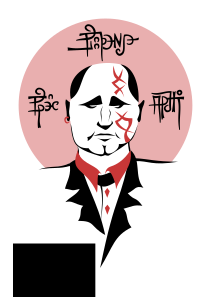
\includepdf[pages={1}]{pic_ValdisJin.pdf}
\newpage
\thispagestyle{plain}

Пропагандистский плакат, изображающий Валдиса Хина, Диктатора Единой Друзы (Гарда Викка), Судью Истории, главу Чашевого Вече.
Надпись гласит:
<<Свобода, Истина, Процветание>>.

Внешность Валдиса в значительной степени приукрашена.
Лысина и полнота считались признаками мужественности и богатства.
По сохранившимся описаниям, лысины у Валдиса не было, и по сложению он был, как и его солдаты, достаточно сухим и мускулистым.
Скорбящее выражение лица и капланский воротник были призваны подчеркнуть его связь с капланами.
Серьга в правом ухе --- символ моряка, намёк на основной источник доходов Диктатора.
Татуировка из четырех букв Х --- известный девиз викканских воров <<Не удержит цепь бродягу>> --- также являлась сигналом: Валдис активно пользовался своими связями в преступном мире.
% ----- PICTURE: VALDIS JIN PROPAGANDA POSTER -----

\chapter{Друза Крепостей}

\section{Телескоп}

Ценного барахла больше не было.
Остался лишь телескоп, сиротливо стоявший посреди развороченных мешков, отодвинутой мебели, осколков стекла...
Вор приник к телескопу глазом --- нечасто увидишь такую штуку.

Следующие двадцать минут воришка провёл совсем не так, как подобало представителю его ремесла.
Открыв рот, он вращал телескоп направо и налево;
подробно рассмотрел Убитого Зайца на Старшей Съедобной Луне, затем Сырную Старуху на Младшей, мельком взглянул на Кольцо Козла и как заворожённый начал пялиться на пылающий Дальний Лимб.

Вдруг чёткую округлость Дальнего Лимба заволокло что-то мутное.
Облако?
Чертыхнувшись, воришка выкрутил регулятор телескопа, пытаясь разглядеть странное препятствие.
Секунда --- и он, подхватив мешок с награбленным, сиганул в окно.

Спустя десять минут в Винокурнях забили колокола, знаменующие вторжение.

\section{Приземление}

--- Да какого дьявола, --- недовольно сказала Ангарьель, складывая глайдер.
Винокурни надрывались колокольным звоном.
--- Какая, скажите мне, сволочь нас заметила?

--- Ты уверена, что это из-за нас? --- сомневалась Курц.

--- А из-за кого ещё колокола будут звонить <<вторженцев>>?
Какой-то пастух в горах увидел кригервинкель и оповестил всех.
Ашита!

--- Да, легат?

--- Свяжись с примой.
Мне нужен чёткий приказ, что делать дальше.
Мы не пройдём до Экзома по чисту полю.
Уже вся Гарда Викка встала на уши, не говоря о Картеле.

\section{ДиС}

--- Что произошло?

--- Поймали члена ДиС, аккурат когда он наносил надпись с угрозами на стену штаба.% D.o.D.
Выяснилось, что их трое.
Завязалась драка, и легата убили.

--- Легат --- урожденный бог?
Я не знала.

--- Клан.

--- Дорге?

--- Да, легат, --- тихо сказал Ашита.

--- Этого только не хватало, --- буркнула Ангарьель.
--- Активисты устранены?

--- Они сбежали, легат.

--- Передай их данные всем, в отношении них действует параграф 14.

Ашита заулыбался.
Курц вдруг поняла, что впервые видит на его хмуром небритом лице улыбку.

--- У вас нет таких полномочий, легат.

--- Ответственность беру на себя.

--- Да, легат, --- Ашита поклонился и пошёл к выходу.

--- Ашита, --- окликнула его Ангарьель.

--- Что-то ещё, легат?

--- Я из бесклановой серии урождённых демонов, уроженка Капитула.
Но я знаю, насколько важна семья.
Я не дам в обиду клан Дорге.
Мне всё равно, боги вы или демоны.
Если понадобится, я буду за вас сражаться.

--- Вас понял, легат, --- Ашита с той же непонятной улыбкой поклонился и вышел.

\section{Нас достаточно}

--- Слишком мало, --- пробормотала Ангара, держась за лоб.
--- Нас не хватит для атаки.

--- Нас достаточно, --- вдруг подал голос Ашита.

--- Нас достаточно, --- откликнулись ещё несколько легионеров.
Курц успела заметить Фумиэ и...

<<Фумиэ?>>

--- К дьяволу, --- кивнула Ангара.
--- Попробуем пройти садами, а там видно будет.
Переоденьтесь в местную одежду и отработайте случайные взаимодействия.

\section{Центр города}

Однако оказавшись на оживлённой улице, Курц поняла, что её предосторожности были излишни --- здесь было такое количество причудливо одетых людей, что её обычный фиолетовый тюрбан и полосатая куртка совершенно не выделялись.
Были и гордые классические костюмы, и павлиньи перья, и художественно изорванные рабочие штаны с заляпанными краской рубахами.
Некоторые люди были почти обнажёнными, другие, наоборот, закутаны с головы до ног в непроницаемо чёрные ткани.

<<Воинственны и опасны>>?
Курц видела лишь разнеженных людей, которые испуганно обсуждали вторжение.
Одни говорили о том, чтобы сбежать, другие надеялись, что им помогут военные, третьи шикали на говорящих, боясь наказания тирана.
Ни один из них, судя по всему, в жизни не держал оружие, их руки привыкли к письму, дорогим тканям и изысканным столовым приборам.

Солдаты, которые распихивали горожан в толпе, были совсем другие: преждевременно постаревшие, но крепкие, с глазами хищных птиц и деревенским говором.
Валдис набирал солдат в деревнях, среди голодающих и невежественных, и они служили ему ревностно, без капли сомнения.
Но это всё ещё были не Фоу-Ф.

\asterism

Трущобы начались внезапно.
Повинуясь красочному указателю, Курц просто свернула с сияющего, пышущего жизнью проспекта на убогую улочку с домами-развалюшками.

<<Это точно центр города?>> --- начала сомневаться Курц.
Вокруг, куда ни кинь взор, были лишь кучи мусора, развалившиеся жилища и лужи.
И над всем этим сияли не такие уж и далёкие золотые купола.

Вскоре впереди появилось здание больницы.
Курц смотрела на него, выпучив глаза.
Выбитые стёкла с торчащими острыми осколками, решётки, листы бумаги и тряпки вместо стёкол, плесень...
В таких развалинах невозможно было излечиться от чего бы то ни было.
Над входом висела полусгнившая табличка <<Больница свят...ни Харгарны, матери...>>

--- З дарохи, --- рявкнул ей мужчина, одетый в грязно-белый ситцевый халат.
Он тащил полуносилки с покрытой рвотой очень полной женщиной.

Курц прислушалась.
Вокруг звучал эрденлид --- очень странный, непривычный, но всё-таки понятный.

<<Здесь квартал выходцев с Хербст?>> --- предположила Курц.
Хотя нет, сомнительно --- эрденлид в числе прочих языков звучал и на чистых улицах.

Курц прошмыгнула в здание через огромную дыру в стене, едва не оставив свою кровь на ржавых металлических штырях.
Перед ней лежали стонущие, кричащие, истерически смеющиеся люди.
Пахло бродящей мочой и экскрементами.

Лежавшая у окна оборванная девушка вдруг захрипела и забулькала.
Она чем-то напоминала саму Курц лет на десять младше --- ожоги на лице, отсутствующий глаз, перетянутый рот.
Курц с ужасом глядела, как изо рта у девушки бежала красноватая пена.
Она задыхалась на глазах...

--- Спырт, --- распорядился рядом врач, выведя Курц из состояния шока.
--- Двадцать мыллылытрав на капэльныцу, срэдная струя.
Живэе, Сьаомэй, эта атьок льохк'х!
Нэ, ты нэ Сьаомэй.
Гдэ эта ратазэйка?

Курц быстро подала врачу спирт и шприц, стараясь не глядеть на больную.

--- Что нада? --- осведомился врач, не глядя на Курц.
Его костлявые пальцы набирали спирт из банки как будто сами по себе.
На указательном пальце левой руки синела татуировка в виде трёх...

--- И трескались губы на ветру, --- тихо сказала Курц.

Врач нервно оглянулся и забормотал под нос какие-то грубые ругательства.

--- Ты зачэм суда прыпёрлас? --- зло прошипел он. --- Хочэш, чтобы мэньа павэсылы?

\asterism

--- Почему ты помогаешь вторженцам?

--- Кто угодна лучшэ, чэм Валдыс, --- буркнул врач.

--- Ну да, мы ведь сюда прилетели, чтобы выпечку раздавать, --- фыркнула Курц, получив от собеседника выразительный взгляд исподлобья.

\section{Проповедник}

--- Опять Свидетели Того, --- буркнул кто-то.
--- Хорошо, что их Валдис приструнил.

--- Мы --- пена морская, мы --- пустота, выглядящая полной, мы вышли из яйца, взбитого Тем Самым, и от пахталки до трапезы мы лишь пытаемся сохранить форму, которую нам придал Кулинар.

--- А потом нас переварят и высрут, --- ввернул юноша в чёрной шляпе.
Все захохотали.

--- Погодите, неверные! --- взревел проповедник, потрясая волосатыми кулаками.
--- Сойдёт на вас кара с горных вершин.
Разрушен будет город, и Ангел Смерти пролетит над ним на алых крыльях!

--- Иди-ка сюда, --- вдруг под руку проповедника взял солдат и отвёл его в сторону.
--- Что там за кара?

Раздался глухой удар и вскрик.

--- Так что за кара? --- продолжал солдат.
Ещё вскрик.

--- Пожалуйста, не надо!

--- Не надо что? --- осведомился солдат.
Снова вскрик, жалобней и пронзительней прежнего.
--- Народ не надо смущать, лодку не надо раскачивать, ты это хотел сказать?

--- Да! --- прорыдал проповедник.
--- Да!

--- Повтори!

--- Лодку не надо!.. (вскрик)
Лодку!.. (хруст и вскрик)
Пожалуйста!
Пожалуйста!..
Народ не надо раскачивать!
Не надо раскачивать!
Пожалуйста!

--- Ещё раз тебя здесь увижу, отправлю прямиком к твоим богам.
Ты меня понял?

--- Он всё понял, он понял! --- из толпы выбежал молодой человек в странной одежде.
--- Это мой отец, у него с головой не всё в порядке.
Простите его.
Я его заберу.
Он всё понял.
Спасибо.
За Валдиса.
За Единую Друзу!
Мы всё поняли.
Спасибо.

С этими словами молодой человек увёл рыдающего проповедника куда-то в кварталы.
У мужчины был разбит нос, заплыл глаз, а его рука безжизненно болталась, словно её вывихнули из сустава.

--- Дитя моё, я пострадал за Веру, --- бормотал мужчина.
--- Не следовало тебе вмешиваться, ты только начали путь...

--- Этот солдат тебя бы убил, отец, --- тихо ответили человек.
--- Братья Сова были осуждены за чтение запрещённых книг на вечное заключение, а сегодня я услышали новость, что их убили в тюрьме другие заключённые.
Закон больше не защищает нас, а значит, мы должны быть осторожны.

--- На всё воля Того, --- отвечал проповедник.
--- Это испытание нашей веры.
На всё воля Того.

--- И на мои слова тоже, --- с некоторым раздражением ответили человек.
--- Я люблю тебя, отец, так же, как люблю Того.
Нас и так мало, кто будет распространять свет Веры, если не ты?

Солдат, покачав головой, поправил кирасу и пошёл дальше.

\section{Публичная казнь}

--- Кто ты? --- спросил его человек с блокнотом.

--- Я Вылемуш Хань из братства Фоу-Ф, --- сказал мужчина.
--- Не зачат, но найден, урожая шестнадцатого года.

--- Что ты сделал? --- продолжал судья.

--- Я сдался в плен листопадникам, презрев законы братства.

--- Что гласит закон братства?

--- <<Изгнать пленённого без борьбы>>.

--- Виновен ли ты?

--- Виновен.
Да накажет меня Тот.

Человек рядом лениво махнул кувалдой и разнес связанному голову.
Толпа завизжала от страха, многие бросились наутёк.
Видимо, для многих этот исход был неожиданностью.
Однако на этом представление закончилось --- наёмники молча ушли, оставив изуродованный труп на площади.
Никто не решился к нему подойти.

--- Что они делают? --- шептала женщина рядом с Курц.
По её щекам текли слёзы гнева.
--- Посреди бела дня!
На Соляной Площади!

--- Все и так знали, как они поступают с отступниками, --- намекнул ей кто-то.

--- Если он нарушил закон, он должен быть осуждён по законам Единой Друзы!

--- Успокойся, --- ответил её спутник.
--- Законы Валдиса не для его gorlosekou, а только для нас.
Пошли отсюда.
Отлично погуляли.

--- А что они обычно делали? --- спросила Курц, изо всех сил стараясь подражать анастасийскому выговору.

--- Ты откуда вылезла? --- осведомилась худая как кость высокая женщина.
--- Да serezali бы его прилюдно, и дело с концом!
Десять раз уже такое бывало!

--- Serezali?
Что это?

--- Палку бы взяли и отходили его по хребту.

--- А, вы тут все пришли посмотреть, как его бьют? --- презрительно процедила Курц.
--- Вы заслужили то, что увидели.

--- Ты откуда сама-то, holudina? --- вдруг спросила женщина.
--- Govor какой-то незнакомый.
Эй!
А ну вернись!

Но Курц, вполголоса ругая себя за неосмотрительность, уже бежала проулками до подземного хода.

\section{Хуга}

Преследователи не отставали.
Похоже, они пустили по следу собак.
Курц не видела их, не слышала лая, но печёнки её трепыхались, как новорождённые птенцы совы в гнезде.
Точно так же как тогда, в юности, когда мама тащила её за руку через сумеречный лес.

--- Мама, я их не вижу, --- жалобно пищала Курц.

--- Не останавливайся, --- хрипло ответила мама.
В её голосе звенел ужас.
В тот же миг далеко позади раздался волчий вой...

...Курц торопливо высыпала на дорогу смесь, которую ей дал Йон Звездочёт.
Её руки тряслись.
Затем, не удержавшись, чихнула от острого запаха и побежала дальше.

<<Направо>>, --- бессловесно крикнул ей инстинкт.
Курц подчинилась не раздумывая.

Зазвенел колокольчик у двери, и деревянная дверь мягко захлопнулась.
Курц заморгала, вглядываясь ослеплённым слезящимся глазом во тьму помещения.
Два круглых стола, несколько плетёных из травы кресел, длинный столик со множеством бутылок, банок, чашек...

<<Питейное заведение>>, --- догадалась Курц.

--- Что будешь пить, девушка? --- голос из угла подтвердил её догадку.

--- Кирш, --- ляпнула Курц на эрденлиде.
Не успела она покрыться холодным потом от собственной глупости, как за стойкой знакомо хлопнула пробка.

Курц быстро оглянулась и села на высокий стул у стойки.
Хозяин оказался полным, лысеющим и седеющим мужчиной с густыми усами и бородой.
На нём был клетчатый жилет в красно-зелёную полоску и цветастый шейный платок.

--- Не самый лучший, --- благожелательно сообщил хозяин, наливая напиток в стопку.
--- Без той шоколадной нотки, которая есть у настоящего тортойсайского кирша.
Не горчит водянисто, как волькейский.
Но есть в нём что-то...

--- ...огнистое, --- закончила Курц.
Кирш пылал в стопке, как пламя свечи, игриво облизывая темнеющий в доске стола сучок.

--- Именно, --- пробасил хозяин.
--- Твои предположения?
Ты вдохни, вдохни...

\ml{$0$}
{Курц постаралась приглушить бешено колотящееся сердце, поднесла стопку к носу и медленно вдохнула пряный спиртовой запах.}
{Kurz tried to rein in her thundering heart, held the shot to her nose and slowly inhaled spicy alcohol odor.}
Солнце за окном стало другим --- оранжевым, ласковым.
Зазвенели ручьи, защебетали яркие птицы, проступили в хрустально-чистом воздухе далёкие очертания Тортойсы, освещённые весёлыми бликами Низины...

--- Хербст, --- наконец сказала она, уже не пытаясь скрыть акцент.
\ml{$0$}
{--- Дахайм-ам-Незен, вишнёвые сады Старого Лога.}
{``Daheim-am-Nezen, cherry gardens of the Old Hollow.}
Кажется, они добавляют в брагу ещё и лепестки.
Выдержка больше десяти лет.

--- Одиннадцать, --- чуть удивлённо ответил хозяин.
\ml{$0$}
{--- Так-так.}
{``Well-well.}
Кажется, я имею дело с истинной ценительницей.
\ml{$0$}
{Выпивка за счёт заведения.}
{Drink on the house.}
\ml{$0$}
{Как насчёт?..}
{What about a---?''}

--- Мне только это, --- быстро сказала Курц, сняла маску и одним махом осушила стопку.
--- Сгодится, чтобы успокоить нервы.

Мимо замызганных окон пробежали двое --- тёмная одежда, револьверы наготове, один ведёт лохматого худого пса.
Оглянулись по сторонам и побежали дальше.

--- Не волнуйся, сюда они не зайдут, --- Курц уловила в голосе хозяина, словно в волькейском кирше, лёгкую горечь.
\ml{$0$}
{--- Никто сюда не заходит последние полгода.}
{``People haven't come in here for the last half a year.}
\ml{$0$}
{Не зайдут и они.}
{Neither will they.''}

\asterism

--- Так значит, прилетела? --- хозяин добродушно хмыкнул.
--- Одна или вместе с этим отрядом с Вольке?

--- Одна, --- быстро сказала Курц.
--- Кружным путём через Змейевиче.

--- Мне плевать, --- хозяин махнул рукой.
--- Я рад всем, кто соблюдает тишину и платит за выпивку.

Курц торопливо порылась в карманах.
Ни платинки.
Вот это номер...

--- Не переживай, --- сказал хозяин, увидев её неудобство.
--- Я же сказал --- за счёт заведения.
Расскажи, откуда эти шрамы.
Впервые вижу человека с лицом смерти.

--- ...Вот так я потеряла маму, --- закончила Курц, утирая неведомо откуда взявшиеся слёзы.
--- Просто вот так --- раз и нет.

--- Я потерял жену, --- ответил хозяин, жуя губу.
--- Тоже tuba fulminata.
Праздновали с ней картонную свадьбу, да день рождения сынишки --- совпало так.
Умерла она наутро.
Сына я растил один.
Мальчуганом был неприметный, мужчиной тоже, зато здоровый.
Знаешь, он такой спокойный, серьёзный, но пошутить любит, крепкий как дуб, твердолобый, скуластый, настоящий солдат, и есть в нём в то же время что-то от его матери.
Глаза, улыбка.
Я говорил ему, говорил --- учи крылья, сынок, будешь мастером.
Мастера ведь --- ууу...

--- Что? --- не поняла Курц.

--- Летишь куда хочешь, --- мечтательно пояснил хозяин.
--- Живёшь где хочешь.
Пьёшь напитки прямо там, где они выросли и были дистиллированы, а не довольствуешься тем, что привезли контрабандисты.
Оставляешь за спиной Друзы, словно деревеньки на обочине дороги.
И самое главное, Курц, --- хозяин ткнул в неё пальцем, --- вы свободны выбирать себе дом.
Поистине свободны.

Курц уже хотела открыть рот и сказать пэну Хуге, что хук и глайдер так не работают, но промолчала.
В его глазах было столько всего...
Да и у неё самой возникли сомнения, странные вопросы.

<<Если мама умела летать, зачем она вообще прожила столько лет в городе, в котором её не ценили?>>

--- А он что, глупый?
Подался в солдаты.

--- Кто? --- не сразу поняла Курц.
--- Ааа, сын ваш?

--- Да, Вылемка, --- кивнул пэн Хуга.
--- Просто в один день сказал, что уходит.
В нашей глуши, как видишь, не заработаешь особо, вот его дружки-то и сманили на деньги.
Всегда с дружками ходил, и здесь пошёл.
Слал мне письма на гербовой бумаге, и деньги слал.
На его деньги, считай, я этот трактир и построил.
Чтобы мы с ним кормились, когда он из возраста выйдет.
Только...

--- Только что?

--- Да с Фоу-Ф он связался, Курц, --- тихо сказал хозяин.
--- Говорил я ему --- не Валдису служи, служи Единой Друзе, и держись подальше от этих отморозков.
Да впустую всё.
Боюсь, не закончится это добром.

--- Как зовут? --- голос Курц опасно повысился.

--- Хуга, --- хозяин явно удивился смене темы.
--- Хуга Хань.
Там написано на стене, видишь?

--- Не вас.
Сына как зовут?

--- Говорю же, Вылемка.
Вылемуш Хань.
Почему ты снова плачешь?
Я тебя расстроил?

--- Курц, --- раздался за спиной знакомый голос.
Она и хозяин вздрогнули одновременно.

--- Когда вы вошли? --- в голосе пэна Хуги прозвучало замешательство, которое не могло скрыть напускное радушие.
--- Я не слышал колокольчика...

--- Я заглушила колокольчик, --- нетерпеливо ответила Ангара.
--- Курц, мы тебя по всей деревне ищем, а ты здесь бухаешь.

Курц смотрела на чёрный приземистый силуэт Ангары, остро ощущая ужас, переливающийся под лопатками.
Это был словно дурной сон из детства --- крохотный хрупкий силуэт на фоне освещённого окна, пришедший ниоткуда.
Ни лица, ни глаз, только ужас, веющий во все стороны, и замерзающий в горле истошный крик.

--- Он тебя раскрыл, верно? --- спросила Ангара на эрденлиде.
Её силуэт потянулся к поясу.

--- Нет, --- быстро ответила Курц, совладав наконец с гортанью.
Она подошла к баронин и положила руку ей на ладонь, уже схватившую револьвер.
--- Всё в порядке, баронин.

--- Курц, --- в голосе Ангары слышалась почти материнская ласка.
\ml{$0$}
{<<Я прекрасно знаю, что ты врёшь>>.}
{\textit{I know for sure that you're lying.}}

Курц смотрела на Ангару сверху вниз с вызовом.
\ml{$0$}
{<<Да, я вру тебе, и мне не стыдно>>.}
{\textit{Yes, I'm lying to you, and I don't feel ashamed.}}
\ml{$0$}
{Ей и правда не было стыдно.}
{She really didn't.}
\ml{$0$}
{От чего ей \emph{было} стыдно, так это от взгляда пэна Хуги --- два кротких голубых глаза под редкими седыми бровями.}
{The thing she \emph{felt} ashamed of was Pen Huga's look---two meek blue eyes under sparse grey eyebrows.}
\ml{$0$}
{В этом взгляде не было страха, не было злости, лишь лёгкая обида от того, что странница, которую он угостил хорошим киршем, его обманула.}
{There was no fear, no anger, only a little wound because of the stranger, who he treated to a good kirsch, and who deceived him after.}

\ml{$0$}
{--- Тебе пора, --- сказал он с той же волькейской горечью.}
{``It's time,'' he said with the same Wolke bitterness.}

--- Спасибо, --- выдавила из себя Курц и, аккуратно убрав руку Ангары с револьвера, вытянула её за дверь.
Колокольчик снова звякнул, и дверь мягко захлопнулась.

\section{Экзом}

И двойным венцом неприступных Винокурен были городки Керивидд и Харгарна, носящие исторические названия Протеом и Экзом.

Экзом был резиденцией тирана.
Крылья Винокурен надёжно прикрывали его с севера и востока, основная часть города находилась на возвышенности, вне досягаемости метательного оружия.
В Харгарну городок переименовал сам Валдис Хин, дав ему имя своей матери.
Называть Харгарну Экзомом строго запрещалось, преступники наказывались по всей строгости.
Кто переименовал ставший царским музеем Керивидд, помнили лишь историки, но, вне всякий сомнений, история была не менее глупой.
Впрочем, название второго города столь строго не блюли и на именование его Протеомом смотрели сквозь пальцы.

Курц невольно залюбовалась крохотным Экзомом.
На Хербст такого великолепия не было.
Ей вдруг до смерти захотелось пройтись по саду, погладить тропические цветы и мягкую траву, которые непонятно как росли и цвели прямо в горном снегу.
Поваляться на аккуратной тропинке, потискать толстого кролика или фазана, которые шныряли по зарослям...

Желание пропало без следа, едва в кустах показался солдат в полном облачении.
Сад был напичкан ими, как пирог курицей.

<<А ведь армия Ордена даже до города не дошла, --- отметила Курц.
--- От кого же ты защищаешься, Валдис Хин?>>

Она пригляделась ещё раз.
Да, это сниффшутцер, или сниффер --- солдат с высокоточным дальнобойным огнестрелом.
На Хербст такие звери не водились, их амуниция и обучение чересчур дорогостоящие.
Даже рожок патронов стоит целое состояние, не говоря уже об оптике.

<<Надо бы раздобыть парочку, когда спустимся, --- отметила про себя Курц.
--- Расходников на них не напасёшься, но всё равно в хозяйстве пригодится>>.

\section{Лавина}

--- Есть одна возможность, --- сказала Ангарьель.
--- Но для этого нам потребуется мастер хука и глайдера.

\asterism

--- Нет! --- Курц швырнула исписанный лист бумаги на стол.
--- Ни за что!

--- Тогда нам крышка, --- спокойно констатировала Ангарьель.

--- Ты хоть понимаешь, сколько людей погибнет?

--- Дорогая, я тебе уже сказала --- решение зависит только от тебя.
Никто из нас не переберётся через эти скалы.
Мы много чего умеем, но не настолько.

--- Ответь на мой вопрос, Ангарьель!

--- Вопрос риторический, и ты это знаешь.
Ещё раз --- меня переубеждать не нужно.
Решение целиком на тебе.

Курц плеснула себе в кружку кирша из графина и выпила его залпом.
Затем ещё одну.
И ещё.

--- Ты таким образом саботируешь восхождение или что? --- Ангарьель с интересом наблюдала за Курц.

--- Я таким образом успокаиваю нервы.
Объясни мне, каковы ставки.
Я должна знать, чем рискую кроме своей чистой совести.

Ангарьель подошла к окну и отодвинула занавеску.

--- Подойди сюда и посмотри.

Курц подошла и вгляделась в раскинувшийся в долине город.
Башенки с золочёными куполами, аккуратные домики с черепичными крышами, пёстрые, похожие на сарландские ковры рынки.
Щебетание птиц, радостные людские крики, блеяние козлов...
Прямо над всем этим ослепительной красотой сиял Экзом.

--- Моё первое тело родилось далеко отсюда, --- сказала Ангарьель.
--- У нас была особая программа воспитания, курсы заботы о теле и психике, курсы правильного общения.
Курсы, курсы, курсы, теория и практика.
Всё, что необходимо для жизни в мирном, красивом, пёстром городе, в нас вложили перед тем, как превратить в орудия войны.

--- Что... --- Курц запнулась.

--- Да-да, понимаю, звучит странно.
Истинная цель моего обучения была в том, чтобы маскироваться под вас, выполняя приказы.
Даже во взаимодействии с вами мы должны быть эффективными.
Я поняла это совсем недавно, когда ты рассказывала про свою маму, про своих друзей, учителей, знакомых.
Для меня это в новинку.
У меня были братья и сёстры, но не было семьи.

--- Очень трогательно, но какое отношение это имеет к тому, что я должна сделать?

--- Мы такие же, как и они, Курц, --- Ангарьель небрежно подбросила в руках нашивку Картеля.
--- Ничем не лучше, ничем не хуже.
\ml{$0$}
{Мы будем вас доить, они будут выкачивать из вас кровь.}
{We milk you, they make you bleed.}
И когда я говорю <<мы>>, я не имею в виду себя --- едва планета перейдёт под знамя Ордена, на тёплое место командующего планетарными силами посадят послушного Капитулу теоретика, а меня отправят в новую мясорубку, символически повысив мой ранг до секунды.
И это будет моим карьерным потолком, если я и дальше буду хорошим солдатом.

--- Переходи к делу, Ангарьель.

--- Тебе придётся сделать выбор между лёгким и тяжёлым.
Ты можешь отойти сейчас в сторону, спасти этот цветущий город и отдать планету Картелю.
Либо ты можешь переступить через свою совесть, залезть на гребаную скалу и дать мне шанс.
Выбор, который коснётся меня, тебя, мои легионеров и жителей этого города.
Для всей остальной планеты принципиальной разницы не будет.

--- Ты хочешь, чтобы война прекратилась?

--- Да.

--- Тогда сдайся, --- предложила Курц.
--- Война прекратится.
Но мы же уже знаем, что ты ответишь, верно?
Ты пытаешься использовать против меня правду.
Тактика хорошая, не знай я, кто ты внутри.

--- И кто я внутри?

--- Солдат.

Ангарьель отвернулась и прикрыла лицо руками.

--- Скажи правду ещё один раз, --- продолжила Курц.
--- Ты хочешь вырваться из этого порочного круга?

--- Я не смогу, --- глухо ответила Ангарьель.
--- Люди находятся в неведении о том, чью сторону они выбрали.
Сторону выбирают за них.
Я, ты, иерархи фракций --- все те, кто видят чуть дальше горизонта.
Но я, демон, легат терция Ордена Преисподней, не сделать выбор не могу.
И никто из демонов не может этого избежать.

--- Ты хочешь вырваться из этого порочного круга? --- настаивала Курц.
--- Ты хочешь жить другой жизнью, в которой будет созидание, а не разрушение?

--- Не имеет значения, что я хочу.
Важно лишь то, что я могу.

--- Ответь --- да или нет?

--- Да.

Курц налила себе ещё кирша, понюхала и с отвращением выплеснула его в открытый ящик шкафа.

--- Подготовь свой отряд, --- сказала она.
--- Я превращу этот город в руины.

\asterism

--- Что с ней? --- шёпотом поинтересовалась Курц.

--- Это Ксения, наш визор, --- ответила Ангарьель обычным голосом.
--- Она всегда такая.

--- Что значит всегда? --- так же шёпотом возмутилась Курц.
--- Девчонка мёрзнет на голом снегу!

--- Не мешай ей, пожалуйста.
И можешь говорить в полный голос --- она визор и всё равно тебя слышит, даже если бы ты стояла на пятьдесят метров дальше.

--- Да что вы за нелюди! --- взорвалась Курц.
Она вытряхнула из рюкзака одеяло и обернула Ксению.
Та вздрогнула и обратила к Курц непонимающие слепые глаза.

--- Привстань, --- скомандовала Курц.
--- Давай, девочка.
Тебе теплее будет.

Ксения бездумно выполнила просьбу.

--- Как тебя зовут? --- отсутствующим голосом спросила девушка.

--- Курц Штайгер, --- ответила женщина.
--- Тебе теплее?

--- Не знаю, --- ответила Ксения.

Курц присела и обняла Ксению.

--- А сейчас?

--- Не знаю.
Мне нужно работать.

--- Я тебе не мешаю, Ксения?

--- Не знаю.

Ксения положила руки на бёдра в молитвенном жесте и прикрыла опалесцирующие глаза.
Её голова опустилась, спина расслабилась, и Курц пришлось поддержать девушку, чтобы та не упала.
Курц без труда узнала это состояние --- демон Ксении начал интенсивно собирать информацию.

\section{Ксения}

Ксения ходила за Курц хвостиком уже несколько дней.
Она ощупывала волосы, плечи, её не смущали ни запах Курц, ни обгоревшее, похожее на череп лицо.
Дошло до того, что за обедом Ксения сидела у Курц на коленях и ела с ложечки.
Курц, которой всегда не хватало тактильного контакта, не возражала.
Вначале она испытывала к девушке исключительно материнские чувства, но в один день с некоторым недовольством почувствовала ощутимое сексуальное возбуждение от тяжести упругого девичьего тела на своих бёдрах.

--- Расслабься, --- ухмыльнулась Ангарьель, заметив неудобство Курц.
--- При длительной тактильной депривации это нормально.
Потом пройдёт.
Хотя я бы её трахнула.
Она возражать не будет.

--- Да в том-то и дело, что возражать она не умеет, --- проворчала Курц.
--- Если не можешь сказать <<нет>>, твоё <<да>> ничего не стоит.
Я не знаю, откуда она, но обращались с ней там паршиво.

Курц настолько привыкла к постоянному присутствию Ксении, что начала шептать --- визор болезненно реагировала на звуки, даже на голос.

Пока Курц собиралась, Ксения всё так же сидела рядом.
Пальцы слепой девушки ощупывали хук, рюкзак, сложенную одежду, предметы гигиены...

--- Ксения, мне нужно уходить, --- ласково прошептала Курц, вытянув из её рук зубную щётку.

--- Ты вернёшься? --- всё тем же эфирным голосом спрашивала Ксения.

--- Конечно.
Ты будешь скучать?

--- Не знаю, --- ответила Ксения.
Её рука ласково, но настойчиво обвилась вокруг запястья Курц.

--- Легат, Курц Штайгер отправляется на задание, --- сказала Ангарьель.
Ксения тут же отпустила руку Курц и съёжилась, словно ожидая удара.
Ангарьель положила руку Курц на плечо.

--- Не заблуждайся на её счёт, --- сказала она.
--- Это не ребёнок.

--- Мне всё равно, --- отрезала Курц и подняла хук.
--- Увидимся завтра.

\section{Восхождение}

<<Дьявол, это не трасса единица, это трасса ноль, --- с восторгом думала Курц.
--- Никаких гарантий, чистая удача.
Мама прихлопнула бы меня на месте, если бы я только заикнулась о желании залезть на такое...>>

\asterism

Она ни разу в жизни не была так высоко от земли.
Каждая Башня была как на ладони.
Где-то вдалеке можно было увидеть даже Гребень Троллей, и упавшую Башню Дьявола.
До облаков было рукой подать;
Курц видела весь их долгий путь --- от Муттермилк через Зелемор, затем извилистая дорога меж венца Гарда Викки, затем циклон, разбросавший облака по всей Друзе...

Курц не удержалась --- заорала во всё горло.
Восторженный крик заметался в заснеженных скалах, словно мышь в горячей клетке.
Казалось, кричала не только Курц --- ей вторили Сабина Штайгер, Карлотта Акст, Лина Коль, все мастера хука и глайдера, которые когда-либо жили на планете.
Мир расцвёл небывало яркими красками, по телу пробегали волны мурашек, Курц чувствовала себя сильной и красивой.
Снег набился ей в куртку и сапоги, но она не чувствовала холода...

<<Однако, надо бы и делом заняться>>.
Курц несколько раз выдохнула, приводя в порядок окутанный эйфорией мозг.

Вот он, тот самый камень, похожий на суслика.
У суслика в голове дыра.
Поместить заряд в дыру и отойти к левой стене... дьявол, или к правой?

Курц вдруг поняла, что момент, непосредственно связанный с её выживанием, совершенно вылетел у неё из головы.
Память была забита извивами трассы, точками крепления, облаками и красотами Гарда Викки, и места для укрытия в ней не осталось.

<<Кажется, Ксения говорила что-то про расщелину между камнями.
Придётся искать>>.

Расщелина нашлась справа.
К счастью, она здесь была только одна.

\asterism

Курц потрясла бинокль и осмотрела подножие скалы.
Лавина сделала своё дело, проложив тропу через городские стены к самому Экзому.
Над всем этим весело сияло полуденное тропическое солнце.

--- А теперь вниз, --- Курц с щелчком расправила красные крылья глайдера, наскоро проверила стропы и, спрыгнув со скалы, понеслась над полуразрушенным городом.

\section{Хин}

--- Ты подойди, --- телохранитель жестом поманил Ангарьель.
--- Мастер останется там где стоит.

Ангарьель подошла к Хину:

--- Я пришла сказать вам, что...

Фразу прервал выстрел.
Хин только начал заваливаться, когда Ангарьель небрежным движением перерезала горла троим охранникам.

Вскоре дым рассеялся.
Хин лежал на полу, корчась в предсмертных судорогах.
Его лицо превратилось в кашу из плоти и костей.
Ангарьель подняла нож для конвертов и перерезала Хину горло.

--- Твоё правление окончено, Валдис Хин.
Пойдём, Курц.

\section{Верность}

Кассия повела плечами.
На её лице замерло злое выражение, немыслимое для ребёнка семи лет.

--- Я должна была проснуться только через одиннадцать лет, но из-за этого бардака пришлось сделать это сейчас, обрекая своё тело на стремительное старение.

Кассия выразительно показала детской ручкой на свою голову.
Среди золотистых волос проглядывали проплешины.

--- У меня создалось впечатление, что вы, Тальяна, захватили полномочия легата прима.

--- Полномочия были переданы мне легатом перед его смертью, прима.

--- И у вас есть доказательства? --- требовательно спросил детский голосок.

Ангарьель прикрыла глаза.

--- Допустим, --- нехотя согласилась Кассия.
--- В любом случае это проступок, который должен быть рассмотрен ранговой комиссией.
У вас не было разрешения на проведение этой операции.

--- Не было никого, кто мог бы выдать мне подобное разрешение, прима.

--- Значит, не надо было делать ничего!
Вы впервые в поле?
И ещё.
До меня дошли слухи...

Кассия перевернула лежащие перед ней бумаги.

--- Параграф 14? --- Кассия вздохнула.
--- Вы потрясающе безрассудны, терция.

--- Это были члены ДиС, прима.

--- ДиС?
Данные точны?

--- Не вижу причин им не верить, прима.
Легат был членом клана Дорге.

--- У нас ещё есть клан Дорге?

--- Трое, прима.
Ашита, Киноу и Фумиэ, я специально вызвала их как уроженцев Тысячи Башен.
Они предупреждены, как и вся когорта.

--- Фумиэ из Дорге у вас в когорте?
Этого легионера выгнали отовсюду, о его трусости ходят легенды!

--- Фумиэ трус, но у него есть очень полезная способность --- он сбегает оттуда, где погибают все остальные.
Пару раз мы уже получали благодаря ему ценные данные.
Я его не выгоню.
Разумеется, ничего важного мы ему не поручаем, он идёт балластом.

--- И тем не менее вы отдали приказ и ему?

--- У него к ДиС свои счёты.
Думаю, в этот раз он трусить не будет.

--- Я не буду их выгораживать, если кто-то из них убьёт члена ДиС без суда и следствия!

--- Я отдала им чёткий приказ под моей сигнатурой.
И давайте закончим разговор о ДиС, прима, потому что мы и так знаем, кто что думает и кто что обязан сказать по этому поводу.

--- Эти слова будут упомянуты в отчёте.
Вы совершенно не колеблетесь перед тем, как подставить подчинённых.
Да ладно подчинённых.
Вы подставили ещё и Опаловый Глаз, вынудив её выполнить заведомо преступный приказ!

--- Во-первых, её никто не вынуждал.

--- Она сообщила, что вы ей угрожали.

--- Она скажет всё что угодно, лишь бы её оставили в покое.
Вы как будто первый день её знаете!

--- Важно не то, что я знаю, а как это выглядит для следствия.
Опаловый Глаз сейчас под следствием, и...

--- О, кто-кто, а Ксения выберется, --- парировала Ангарьель.
--- Её лояльность никогда не была под сомнением.
Но что важнее --- она для Ордена гораздо полезнее пушечного мяса вроде меня.
Её в любом случае не отстранят, какими бы правдами и неправдами этого ни пришлось добиться.

--- Откуда эти пацифистские медиавирусы, Тальяна? --- голос Кассии вдруг стал шёлковым.
--- Откуда это <<пушечное мясо>>?
С вами кто-то беседовал на эту тему?

--- Меня зовут Ангарьель, прима.

--- У меня другая информация.

--- Боюсь, моя информация имеет в данном случае приоритет, прима.

Кассия отложила в сторону бумаги и бросила на стол ручку.
Её ножки торчали из кресла, словно у куклы.

--- Не зарывайтесь, Древолаз, --- отчеканила она.
--- Вы идеальны в роли легата терция.
Не заставляйте меня разжаловать вас в центурионы.

--- На каком основании, прима? --- с убийственной вежливостью поинтересовалась Ангарьель.

--- Ваша лояльность уже вызывает сомнения.
Факт, что вы не можете быть верны даже данному вам имени, играет против вас.

--- С какой стати я должна быть верной набору звуков и букв?

--- Тальяна, прекратите немедленно.

--- Ангарьель, центурион.

--- Как вы смеете! --- прошипела Кассия, приподнявшись в кресле.

--- Как смеете вы на подобном смехотворном основании угрожать мне пенальти? --- рявкнула Ангарьель.

--- Значит, оно для вас смехотворное?
Вы уже подобным нарушением субординации заслуживаете расследование!

--- В таком случае вызовите меня на суд, мы с военным трибуном посмеёмся вместе!
Если вы не собираетесь созывать трибунал --- не морочьте мне голову этими бреднями!

Кассия холодным взглядом долго смотрела на подчинённую.

--- Вы свободны, Ангарьель.

--- Прима, --- Ангарьель поклонилась чуть резче, чем следовало, и пошла к выходу.

\section{Неожиданный поцелуй}

Повозившись с замком, Ангарьель наконец открыла дверь своей комнаты и устало завалилась внутрь.
Внутри всё ещё всё кипело от разговора с Кассией.

--- Ты долго, --- Курц встала с кресла и размотала тюрбан.
--- Извини, я пролезла в окно, потому что думала, что ты...

Ангарьель тремя широкими шагами достигла Курц и нежно впилась пухлыми губами в обгоревшую прорезь на месте рта.
Курц медленно начала таять, как лёд на солнце.
Руки Ангарьель аккуратно стянули с неё кушак, расстегнули крепления, узкие ладони змеями проползли в рукава...
Курц уже не слышала ничего, кроме прерывистого дыхания и шелеста медовых волос у ушной дырки.
Бздынь --- застонали пружины кровати, и Курц неожиданно для себя приняла горизонтальное положение.

<<Почему бы и нет, --- подумала женщина, лаская молодое, упругое тело Ангарьель.
--- У меня давненько никого не было.
Просто секс, просто... просто...
Ааааах.
Дьявол.
Дьявол!
Да кого я обманываю.
У меня всё внутри дрожит, когда она меня касается, словно ветряная рябь на водной глади...>>

--- Подожди, малышка, --- шёпотом попросила она, положив пальцы на нежные губы.
--- Подожди секунду.
Погладь меня.
Просто погладь, и я вся твоя...

Ангарьель поцеловала Курц в выжженный висок, прижала её к себе и запустила пальцы ей в волосы.
У Курц в груди медленно нарастали тяжесть и боль, словно открывалась старая рана, словно рушилась земная твердь, отправляя деревья, траву, птичьи гнёзда и лис в чёрную пасть карстовой жеоды.
И с каждым прикосновением Ангарьель солёные реки лились в жеоду, превращая её в прекрасное голубое озеро.

\section{Террористы}

--- Орден Преисподней --- просто террористы.

--- Да, для многих это будет выглядеть как хаос, --- кивнула Ангарьель.
--- Отцы обратятся против детей, внучки пойдут против дедов.
Но это лишь ширма, внешняя оболочка.

--- А ты не думаешь, что то, как вещь выглядит, порой и есть её суть?

Ангарьель на несколько долгих мгновений замолчала, думая, стоит ли сказать то, что вертится на языке.

--- Ты гораздо красивее внутри, чем снаружи, Курц, --- наконец проговорила она.

--- Но ведь внешность отражает мою суть, --- грустно возразила Курц.
--- Я привыкла быть уродливой, быть калекой.
Я сломана внутри.

--- Ты не...

--- Не перебивай.
Я сломана, это правда.
Даже если я шагну за пределы своих возможностей, даже если я сменю десять тел --- моё самое первое искалеченное тело останется со мной навсегда.
Внешнее всегда связано с тем, что внутри.

--- Я достаточно повидала войн, чтобы делать выводы.

--- Ты никогда не видела войну так, как видят её простые жители.
Ты видишь то, что тебе позволяют видеть командиры --- маску войны.
Ты бессознательно дорисовываешь войне лицо, и оно кажется тебе красивым.
Но те, кто никогда не обладал твоей властью и твоими знаниями, будут видеть войну такой, какая она есть, без маски, без дорисованной красоты.

--- Я не вижу другого пути, --- буркнула Ангарьель.
--- Если ты считаешь меня террористкой --- я приму это как справедливую цену за правильный поступок.

--- Скажи, почему ты называешь себя человеческим именем?

Ангарьель непонимающе посмотрела на подругу.

--- Я слышала, как твоя командир называла тебя Тальяной, --- пояснила Курц.
--- Но ты продолжаешь называть себя Ангарой.

Баронесса отвернулась.

--- Это личное.

--- Сколько времени тебе потребовалось, чтобы понять, что ты Ангара, а не Тальяна?

--- Нисколько.
Я просто услышала это имя и поняла, что оно принадлежит мне.

--- Тогда я уверена, Ангарьель, что однажды ты меня поймёшь.

--- Почему?

--- Потому что все самые важные изменения происходят без войны.
Ты просто понимаешь, что новый порядок вещей --- единственно правильный для тебя.

\section{Поцелуй}

--- Я не удержалась и поцеловала тебя тогда, когда ты лежала без сознания.

--- Не удержалась? --- хихикнула Курц.

--- Я сняла с тебя маску, чтобы обработать тебе раны, и...
Если честно, я ожидала чего-то худшего.
А ты...
Ты была похожа на...

--- На грелла?

--- Наверное.
Не на то чудовище, которым пугают детей, а на принцессу греллов --- самую прекрасную женщину из всего их племени.

--- Наверное, это твой демон, --- предположила Курц.
--- Мне все говорили, что моё лицо --- это выжженная дотла деревня.

--- Да, это был демон.
Он экстраполировал твоё лицо и показал мне проекцию.

--- Скажи ему больше так не делать.
Я не хочу, чтобы ты целовала маску.
Даже ту, которую на меня надел твой демон.

Ангарьель прижалась к Курц и погладила обтянутую шрамами грудную клетку.

--- Почему мне с тобой так хорошо?

--- Потому что ты меня любишь, --- прошептала Курц.

--- Я боюсь того, что это значит.

--- Что это значит?
Чего ты боишься?

--- Я не могу чересчур близко к сердцу принимать то, что происходит с людьми.
Иначе я забуду о долге.

--- Зачем нужен долг, если тебе некого обнять по возвращении домой?

--- Поцелуй меня и засыпай.

--- Это приказ, баронин?

--- Это приказ.

\section{Старый друг}

--- Шнелль!
Какими судьбами здесь?

--- Мост наш, --- Шнелль сиял, как Съедобная луна.
--- Работка была нелёгкая, но мы справились.
Возможно, вам понадобится.

--- Что вы сделали, дьявол вам возьми? --- с восторгом спросила Ангарьель.

--- Смыли их к дьяволу, --- ухмылялся Шнелль.
--- Наклон Моста позволял.
Мы оживили трубы от старой водонапорной башни в горах.
Фоу-Ф использовали руины как укреплённый пункт и не ожидали атаки с этой стороны.
Затем, после суток перестрелок на Мосту, мы подключили пожарные шланги и спустили воду с небольшим количеством едкого вещества вниз по Башне.
Те, кто выжил, захотели сдаться.
Жалко, что пленных мы в этот раз не стали брать.
Мы дали Мосту сутки на просушку и пошли по чистенькому.

--- Взорвать бы его к дьяволу, --- сказала Курц.
--- Ничего, кроме худа, от него не было.

--- Знал, что ты это скажешь, --- кивнул Шнелль.
--- Мы заложили взрывчатку, пока шли.
Места знаю только я и пара моих ребят.
Наш инженер сказал, что заложил с запасом --- даже горы не переживут.
Так что Мост простоит ровно столько, сколько нужно нам.
Вы закончили свои дела здесь?

--- Не совсем.
Сколько у тебя людей?

--- Десятая часть населения Хербст, почти все, кто может держать оружие.

--- Ты перевёл через Мост тридцать тысяч человек?!

--- Двадцать одну тысячу, баронин.
Ещё десять тысяч на той стороне, стерегут подходы и доставляют провизию.

--- Мне понадобятся десять тысяч, чтобы закончить дела.

--- Мы к твоим услугам.
Только сразу хочу предупредить: у тех, кто здесь, настрой не самый радужный.
По большей части это люди, потерявшие родных во время бесчинств Фоу-Ф.
Контролировать их сложно.
Они устроят резню при любом удобном случае.

\section{Поле боя}

Город больше не защищали стены.
Войска Листопадной Друзы затопили полуразрушенные Винокурни, словно серая вода.

Анастасийцы сражались как звери.
Записанный в воске голос уже мёртвого Валдиса Хина разносился по городу.
Валдис, как человек предусмотрительный, записал обращения на случай любого исхода мостовой войны, и сейчас из рупоров звучало: захватчики с Хербст убьют ваших детей и изнасилуют ваших женщин.
Бои шли за каждый дом, в каждом подвале разгорались схватки --- викканцы и жители Хербст рубили друг друга топорами, душили рыболовной леской, били поленьями, грызли зубами и выцарапывали глаза ногтями.
Вой раненных и умирающих стоял ужасный --- такого не было даже тогда, когда по Хербст гуляли Фоу-Ф.

<<Где здесь правда? --- думала Курц.
--- Есть ли она вообще?
И, самое главное, что здесь делаю я?
Кто я в этой истории?..>>

\section{Обречённое место}

--- Погуляем вечером?

--- Прости, малышка.
Вечером я буду спать.

--- Как хочешь.
Скоро вся эта красота исчезнет, как только горожане поймут, что Валдис мёртв.
Первыми, конечно, придут мародёры --- вынесут всё ценное и забьют на мясо зверей.
Потом придут разъярённые погорельцы и разнесут всё, что осталось --- оборвут цветы, сожгут картины, сломают статуи, уничтожат всё, что напоминает им о пропасти между хозяевами и рабами.

Курц невольно бросила взгляд на цветущие сады.

--- И через сотню лет, --- продолжала Ангарьель, --- на развалинах обгаженного, разворованного имения сделают такой же музей, как в Керивидде, неуклюже пытаясь воспроизвести эпоху, ставшую историей.
Множество людей будут мечтать её вернуть, глядя на рафинированное великолепие картин и пышный слог плакатов.
Но мы этого уже не увидим.
Наверное, и к лучшему.
Так что сегодняшний вечер --- всё, что у нас с тобой есть, Курц.
Это место обречено.

--- Ангарьель, давай о чём-нибудь весёлом, --- взмолилась Курц.
--- Я и так помираю от этой безнадёги.
Давай погуляем.

--- Я и предлагаю погулять вечером.

--- Не вечером.
Сейчас.

--- Сейчас у меня дела.

--- У тебя всегда дела, --- Курц скрестила руки на груди.
--- И из-за этих дел умирают люди.

--- В чём конкретно ты меня обвиняешь?
Если бы не я, то ты бы не стояла на руинах Винокурен, а лежала бы в руинах Хольца.

--- Хольц справился и без тебя.

Ангарьель хмыкнула и покачала головой, но промолчала.

--- Это не так, легат, --- вмешался Диссонатч.
--- У города были серьезные проблемы с логис...

--- Диса, хватит.
Ей сейчас не нужны доводы разума и факты.
Иди погуляй.

Диссонатч кивнул и вышел.

\asterism

--- Это вы принесли войну, --- глухо сказала Курц.
--- Если бы не пришли демоны, ничего этого бы не было.

--- Давай посмотрим, --- Ангарьель деланно улыбнулась одними губами и встряхнула бумаги.
--- Во время стычек с мародёрами --- такими же горожанами --- погибло двести дружинников, ещё более семисот ранены и искалечены.
Кто это сделал?
Валдис?
Я?

--- Анастасийцы.
На Хербст такого не...

--- Каждый член системы несет в себе её отпечаток.
И неважно, на какой Друзе ты живёшь, кому поклоняешься, на каком языке говоришь.
Каждый человек несёт на себе отпечаток общепланетной цивилизации.
Нельзя отгородиться и сказать, что вы не имеете к этому отношения.

--- Мы не вторгались в...

--- Вы уже на Гарда Викке, Курц!
Вы уже вторглись!

--- Мы защищались от...

--- Ты так уверена? --- буркнула Ангарьель.
--- Посмотри на статистику по битве за Винокурни.
Это жители города.
Убитых --- восемь тысяч, из них тысяча детей.
Раненных --- двадцать одна тысяча пятьсот.
Потеряли глаза, конечности, гениталии, прикованы к кровати --- две тысячи восемьсот.
Умерших от болезней --- пять тысяч.
Да, в городе были больные, которым была нужна помощь.
Умерших от голода и жажды --- четыреста.
Под завалами погибло --- семьсот восемьдесят.
Изнасилованы --- семнадцать тысяч, из них тринадцать тысяч женщин, две тысячи мужчин, девятьсот два ребёнка младше десяти лет и больше тысячи немощных стариков.
Кто всё это сделал, м?
Моя когорта или твои соотечественники?

Курц выхватила из рук Ангарьель листок и, разорвав его на мелкие кусочки, выбросила в окно дворца.
Обрывки весело кружились в напоённом солнечным светом воздухе, оседая на мягкую зелёную траву, и кролики с фазанами уже начали сбегаться к ним, думая, что это очередное угощение.

\section{Падение}

Ветер бешено трепал её волосы.
Крюк уже почти выскользнул из расщелины.
Один взмах рукой, одно усилие --- и впереди лишь дорога до баронства, домик с деревянным настилом и каменной трубой, стук в дверь, удивлённый взгляд Шнелля и кровать, сделанная специально для неё...
Но Курц не торопилась протягивать руку.

--- Командир?

Легионер бросился к краю скалы и лёг плашмя.
Его рука запоздало царапнула камень.
Крюк тихо выскочил из расщелины, и Курц Штайгер, в ужасе закричав, растворилась в тумане.
Спустя несколько секунд крик вдребезги разлетелся о скрытую под мглистой дымкой скалу.

\section{Холод}

--- Мы не нашли её тело.

--- Так ищите ещё! --- раздраженно рявкнула Ангарьель.
--- Оружие, амуницию, обломки, всё, что найдёте, несите мне!

--- Вы ищете что-то конкретное, легат? --- уточнил посыльный.
--- Может быть, какое-то устройство, документы, которые у неё были при себе?
Мы можем задействовать поисковую технику, если будем знать, что искать.

--- Задействуйте что угодно, только принесите мне Курц Штайгер!

Ангарьель захлопнула дверь и упала в кресло, обхватив голову руками.
Резко стало холодно, несмотря на горящий камин;
Ангарьель закуталась в одеяло, но холод упрямо заползал в руки, ноги и горло, грозя добраться до сердца.

И только слёзы, которые лились из голубых глаз, были жарче камина.

\section{Возвращение}

--- Курц, ты жива!

--- Да, я имитировала свою смерть.

--- Но зачем?

--- Чтобы быть с тобой, конечно.
Пойдём.

Курц потянула Ангарьель за руку, но та не сдвинулась с места.

--- Я не понимаю, --- прошептала Ангарьель.

--- Мы уйдём от Ордена, мы уйдём ото всех.
У нас будет домик у озера, огород, сад...

--- Курц, я не могу.
Я служу Ордену.
Я не могу уйти.

Курц отпустила руку Ангарьель.

--- Ты сказала, что хочешь быть со мной.

--- Я хочу, но я думала...

--- ...думала, что я стану террористкой, как и ты? --- холодно завершила Курц.

--- Курц, пойдём со мной.
Мы будем вместе, и у нас будет общее дело, и...

--- Да не нужно мне твоё общее дело, --- буркнула Курц.
По её лицу текли слёзы.
--- Я за тобой пришла, малышка.

--- Я не могу уйти с тобой, Курц, --- прошептала Ангарьель.
--- Я не могу...
Курц, подожди.
Вернись.
Пожалуйста.
Не уходи...

Но было поздно.
Туманы Вольке поглотили Курц Штайгер, надёжно скрыв направление её пути.
Ангарьель упала на колени и взвыла от боли и одиночества, но ей ответило лишь эхо в опутанных туманом скалах.

\section{Эпилог}

Посреди палатки стояла на коленях женщина в цепях.
Её и без того изуродованное, похожее на череп лицо было изборождено обветреными морщинами.
Кудрявые волосы --- наполовину черные, наполовину седые --- были растрёпаны, в них застряли сухие листья и трава.

--- И снова здравствуй, --- поприветствовала её женщина в камуфляже, по виду --- офицер.
--- Как здоровье?
Давно тебя не было видно.
Три года?
Четыре?
Ты стала умнее и хитрее, чем раньше.

Пленница не ответила.
Офицер одним движением сорвала с её шеи красную тканевую маску.

--- <<Охотники на демонов>>.
Серьёзно?
И сколько демонов вы убили?

Молчание.

--- Ты пыталась снять чертежи с аппарата для оцифровки, а также нескольких машин, использующих омега-интерфейс.
Отдам тебе должное, в этот раз направление правильное, но расстояние ты недооценила.
Даже если ваши специалисты поймут принцип (в чём я уже сомневаюсь), то чтобы собрать сколько-нибудь работающее оборудование, вам потребуются огромные производственные мощности.
С учётом ресурсов Тысячи Башен, на это уйдут десятки лет --- даже если бы я вам не мешала.

Пленница вздохнула.

--- Демоны --- это не люди, это сгустки информации.
Ты не можешь уничтожить нас, просто проделав в нас несколько дырок.
Или ты собираешься выявлять демонов среди людей, устроить новорождённым тотальный скрининг, чтобы избежать появления инкарнатов?
Идея не новая, это пытались реализовать в десятках более технологически развитых миров, не получилось ни у кого.
Люди размножаются стихийно.
Тебе не под силу поставить вопроизводство даже под статистический контроль, не говоря обо всём остальном.

Молчание.

--- Из-за тебя погиб Шнелль, --- Ангарьель закатала рукав и показала часики с ёжиком на запястье.
--- Я казнила его лично.
Он пошёл за тобой, потому что верил тебе, как и все остальные.
У тебя был выбор.
У меня выбора не было.

Молчание.

--- Ты понимаешь, что ставишь себе невыполнимую задачу?
Ты отдаёшь себе отчёт, что каждая твоя попытка забирает жизни людей, не принося тебе взамен ничего?
То, что ты собираешься сделать, не под силу одному человеку, не под силу сотне и десятку тысяч тоже.
Твоему телу осталось жить сорок лет, плюс-минус удача, но твои умственные ресурсы подойдут к концу намного раньше.

Молчание.

\ml{$0$}
{--- Я должна тебя поблагодарить, впрочем.}
{``I owe you appreciation, though.}
\ml{$0$}
{Благодаря тебе Капитул отложил мелиорацию Тысячи Башен на неопределённый срок.}
{Because of you, Capitul had postponed melioration of Thousand Towers indefinitely.}
Я регулярно шлю отчёты о чистках и казнях, которые предпринимаются против сторонников неуловимой Курц Штайгер.
\ml{$0$}
{Пока ты борешься, мои легионеры живут здесь, мирно и счастливо.}
{While you're fighting, my leggionaires live their best life here, in peace.''}

Легионер у входа усмехнулся и тут же кашлянул, вспомнив о субординации.

--- Не хочешь говорить --- не надо, --- пожала плечами женщина в камуфляже и обратилась к подчинённому:
--- Отведите её за город, снимите оковы и оставьте там.

--- Хватит!

Отчаянный крик пленницы разорвал пустоту, словно удар молнии.
Женщина в камуфляже подняла брови.

--- Тринадцать раз! --- хрипло выплюнула пленница.
--- Тринадцать раз я попадаю в плен, и тринадцать раз ты меня отпускаешь!
С меня хватит!
Просто убей меня!

--- Я всё сказала тебе еще в нашу третью встречу, --- терпеливо пояснила женщина в камуфляже.
--- Однажды я увидела нечто большее за изуродованным лицом.
И сейчас я вижу нечто большее за твоими бесконечными бесполезными попытками организовать восстание против Ордена.

--- Ангарьель, просто убей меня, --- прошептала пленница.
По её лицу градом катились слёзы, теряясь в извилинах шрамов и морщин.

--- Нет, Курц, --- отрезала женщина в камуфляже.
--- Ты мне нужна.
Легионер, вы слышали мой приказ.

Легионер вздёрнул пленницу на ноги и вывел её из палатки.
Ангарьель осталась одна.

Солнце давно ушло за полдень и наконец заглянуло в проем палатки.
Ангарьель на секунду оторвалась от своих записей и подставила лицо теплому оранжевому свету.
Он был таким ласковым, таким нежным, как...

--- Командир.
К вам пленница, которую вы велели отпустить.
Пришла пешком.
Просит слова.

--- Впустите, --- встрепенулась Ангарьель.

Курц вошла в палатку и остановилась, скрестив руки на груди.

--- Я отказываюсь признавать власть Ордена здесь.

--- Я в курсе, --- пожала плечами Ангарьель.
--- Могла бы приберечь эти слова до своего следующего пленения.

Курц молча встала на одно колено.

--- Я клянусь тебе в верности, Ангарьель.
Я буду делать то, что ты прикажешь.
Я отказываюсь признавать власть Ордена над Тысяче Башен, но я признаю твою власть надо мной.

--- Ты готова к тому, что тебя возненавидят бывшие соратники?

--- На этом свете не осталось никого, чьё мнение меня волнует.

Ангарьель откинулась в кресле и взглянула в оплетённое заходящим солнцем лицо Курц.
Молчание тянулось долго, словно мёд...
Наконец Ангарьель встала на ноги.

--- Легионер, --- позвала она.

--- Да, командир?

--- Отвезите Курц Штайгер в штаб и подготовьте к оцифровке.
Настройте оборудование под мои сигнатуры.
Отправьте сообщение на Капитул: я нашла кандидата на пост командующего вооруженными силами Ордена на Тысяче Башен.

\section{Нос}

Ангарьель долго молчала, не зная, что сказать.

--- Хорошо выглядишь, --- наконец проговорила она.

Курц ухмыльнулась.

--- Ну, я теперь не грелл, --- женщина немного шепелявила.
--- Пока не освоилась с губами.

Ангарьель погладила Курц по грудной клетке.

--- Грудь не сделала?
Тебе и ее могут вырастить.

--- Я отказалась.
Привыкла уже, ну и в моём деле грудь будет только мешать.
Нос пока что тоже мешает... пару раз очень больно стукнула себя по носу... но дышать с ним проще, признаю.

Ангарьель промолчала, смотря на вышитый ворот рубашки Курц.

--- И куда ты теперь? --- поинтересовалась Курц.

--- В поля, --- улыбнулась Ангарьель.
--- В команде Хэм Золотой Посох освободилось место, и я попросилась к ним.

--- Кажется, я уже слышала про команду Хэм.
Диверсанты?

--- Одни из лучших.

--- Я слышала, у них маленькие отряды.

--- Когортами не ходят.
Чаще всего отряд диверсантов --- это три-четыре демона.
Почти семья.

Курц едва заметно улыбнулась.

--- Может быть, найду себя там, --- Ангарьель зевнула.
--- Я не подхожу для административной работы.

--- С чего ты взяла, что для неё подхожу я?

Ангарьель хихикнула.

--- Да мне плевать, подходишь ты или нет.
Я просто не хочу, чтобы ты стала террористкой, как я.

Курц опустила голову.

--- Сейчас у тебя есть хороший шанс принести людям хорошую жизнь.

--- Командующий армией --- это не та должность, которая приносит счастье, --- возразила Курц.

--- Именно та.
Не используй армию без крайней необходимости.
Цени жизни людей и легионеров.
Покажи всем, что мир для тебя важнее всего.
И, что самое важное, шли к волкам приказы свыше, пока есть возможность.

--- Почему я?

--- Никто не знает Тысячу Башен лучше тебя.
Это твоя родина, твои угодья.
И я теперь знаю, что ты будешь сражаться за неё с кем угодно, даже если надежды на победу нет.

--- Как скажешь, Ангарьель.

--- Я не хочу, чтобы ты делала всё это из-за обещания, которое дала мне.
Я хочу, чтобы ты делала всё это, потому что это правильно.

Курц кивнула.
Ангарьель вдруг повела плечами, словно ей стало холодно.

--- Слушай, Курц.
Моя новая работа очень интересная, но и опасная тоже.
Особенно сейчас.
В общем, я...

--- Я знаю, --- сказала Курц.
--- Ты думаешь, что не вернёшься.

--- Да.

\ml{$0$}
{--- А если вернёшься, мы никогда не будем так близки.}
{``And even if you come back, we'll never be as close as we are now.''}

--- Я никогда ни с кем не расставалась, --- призналась Ангарьель.

--- Ты рассталась со мной тогда.

Ангарьель вздохнула.

--- Чёртовы люди.
У нас с вами разное чувство времени и расстояния.
Мы с тобой были на одной планете, Курц, это почти что рядом, да и несколько лет --- это всего лишь мимолётное расставание.
Я знала, что ты где-то здесь, в пределах досягаемости, и это грело мне душу.
А сейчас...

--- Мы уже никогда не будем близки так, как могли бы быть, Ангарьель.
Наш медовый месяц закончился, не успев начаться.

Ангарьель опустила голову.

--- Но чужой ты для меня тоже уже не будешь, --- шёпотом добавила Курц.
\ml{$0$}
{--- Из моего сердца обратной дороги нет.}
{``There's no way back from my heart.''}

--- Почему же ты меня так ненавидела?

--- Я ненавидела не тебя.
Может быть, твоего демона, отнявшего у меня любовь моей жизни...

--- Глупости.
Демон встроился в меня, дал мне знания, помог мне выжить, только и всего.
Глупости говоришь.

--- Для тебя --- возможно.
Будь Ангара Ротештурм обычной женщиной, в ней бы не было верности Ордену, обязанностей, ответственности.
Я унесла бы её в домик на краю света, и пусть весь мир горит пламенем...
Но увы, между нами встали обстоятельства в виде сгустка непонятно чего, в чём нельзя проделать дырок и убить.

Ангарьель кивнула.

--- Я вернусь к тебе, Курц.
Во мне не так-то просто сделать дырку.

--- Если ты не вернёшься, я буду считать себя свободной от данного обещания и уничтожу Орден.

--- Зная твоё упорство... --- поёжилась Ангарьель.
--- Мне и вправду лучше не умирать.

Повинуясь внезапному порыву, Курц подошла ближе и поцеловала Ангарьель в пухлые губы.
На секунду солнце вдруг стало тем, осенним, ласковым;
вокруг закружились в танце чуть влажные золотые листья.

--- Мне не следовало уходить, Ангарьель, --- прошептала Курц.

--- Тебе нужно было время, --- улыбнулась Ангарьель.
--- Мне тоже, похоже, нужно время.
Непонятно для чего, но определённо нужно.

--- Прощай, Ангарьель.

--- Прощай, Пламя Осени.

\section{Карта стратегии}

...После демонизации и пластической операции Ангарьель несколько раз заходила в лазарет навестить Курц.

--- Шести легионерам, которые в курсе ситуации, я приказала молчать, --- сказала она.
--- Так что все будут считать, что ты умерла.
Ты останешься в памяти людей такой, какой они знали тебя при жизни --- непокорённой легендой.
Я думаю, что всем нужны такие легенды.

\ml{$0$}
{--- Принцесса греллов мертва.}
{``The Grello Princess is dead.''}

\ml{$0$}
{--- Да здравствует Пламя Осени.}
{``Long live the Flame of the Fall.''}

--- Паршиво, конечно, это всё.
Лживо.
Но, думаю, я заслужила то, что имею.

--- <<Заслужила>>, --- фыркнула Ангарьель.
--- Ну и дурацкое же это слово, кто его только выдумал...
С меня сняли ранг сразу после присвоения.

\ml{$0$}
{--- Ты снова терция?}
{``Are you tercia again?''}

\ml{$0$}
{--- Снова терция.}
{``Tercia again.}
\ml{$0$}
{Вечная терция.}
{Tercia forever.''}

\ml{$0$}
{--- За самоуправство?}
{``Excess of authority?''}

--- Именно.
Вся эта история с ДиС, потом ты...
При этом в целом трибуны согласились, что действую я в интересах Ордена и лучшего кандидата найти сложно.
Твоё досье пока что идёт в секции пять, гриф <<Истекающая секретность>>.
Легенду тебе придумывают лучшие аналитики.
Это стоит ранга.

--- Наверное, даже ранг --- это не награда, а миссия, --- предположила Курц.
--- Я бы предпочла терцию Ангарьель тысяче легатов прима.

--- Теперь ты меня понимаешь, ---- Ангарьель тепло посмотрела на стоявшего у дверей Ашиту.
Легионер стоял расслабленно, положив смуглые руки на автомат, и наблюдал за порхающей у дверей бабочкой.
--- Я оставлю тебе когорту.
\ml{$0$}
{Доверяй им.}
{Trust 'em.}
\ml{$0$}
{Цени их.}
{Respect 'em.}
\ml{$0$}
{Советуйся с ними.}
{Seek counsel from 'em.}
\ml{$0$}
{Лучшей когорты ты не найдёшь.}
{You can't find a better cohort.''}

--- Примут ли они меня? --- грустно спросила Курц.

--- Я бы не отдала их тебе, если бы они тебя не приняли.
Да, Диса?

Диссонатч молча перебинтовывал Курц руки.
Его потемневшие узловатые пальцы были тёплыми-тёплыми, пробуждая в ней что-то забытое, заставленное нагромождениями эмоционального хлама.
Курц на секунду встретилась с ним взглядом --- в карих глазах под чёрными кудрями тоже замерла теплота...

--- Не уходи от меня, --- Курц зацепила Диссонатча за пуговичную петлю, когда он закончил.
--- Это приказ.

\asterism

Курц уже начала осваиваться со стратегическими модулями.
Проблема --- щёлк --- решение --- щёлк --- новая проблема --- щёлк --- новое решение --- щёлк...

<<Так вот как вы нас сдерживали.
Умно.
Но эта цитадель отнюдь не неприступна...>>

Курц вытащила из стопки бумаг чистый лист и карандаш.
Слабо улыбаясь, она нанесла на карту стратегии первые два узла и соединила их пунктиром.
\ml{$0$}
{Демон тут же подсветил их в её сознании:}
{The daemon immediately highlighted them in her mind:}

\ml{$0$}
{<<Курц Штайгер - - - - - Ангара Ротештурм>>}
{\textit{Kurz Steiger - - - - - Angara Rotesturm}}

\appendix

\chapter{Таймыр: культура без носителей}

\epigraph{
\ml{$0$}
{Если нужно --- возьми.}
{Take if you need.}
\ml{$0$}
{Если хочешь --- отдай.}
{Give if you want.}
\ml{$0$}
{Над Таймыром нет богов, и никто, чёрт возьми, не будет тебя судить.}
{There is no gods upon Tajmeir, and no one's gonna fucking judge you.}
}
{
Надпись на воротах Мастерской Доброй Воли, записанная таймырскими идеограммами.
Друза Таймыр, Тысяча Башен.
}

Друза Таймыр --- единственная необитаемая Друза Тысячи Башен, на которой регулярно появляются люди.
Причина проста --- она связывает Тропический Пояс с Экваториальным Кластером.
За прошедшие века и тысячелетия на Таймыр сформировалась уникальная культурная экосистема, в которую вовлекаются все так или иначе оказывающиеся там люди.

Первым фактором, формирующим культуру Таймыр, является отсутствие привычных способов передачи информации от опытных людей к неопытным.
Смертность на дороге составляет тридцать процентов.
Большая часть погибших приходится на тех, кто страдает хроническими заболеваниями.
Недостаток кислорода, перепады температур более семидесяти градусов, голод (на Таймыр почти отсутствует растительность и крупная фауна) --- суровые испытания для человеческого организма.
Из тысячи переживших этот поход лишь пятеро решались на него повторно, и лишь одному удавалось за жизнь пройти Таймыр три и более раз.
Таким образом, специалистов по Друзе Таймыр в привычном понимании не существует --- есть те, кто её пережил.

Второй фактор --- это асимметрия.
Дорога на север и дорога на юг --- это два разных пути.
Эти пути пролегают между скал и упавших Башен, изолированы друг от друга и имеют совершенно разную культуру.
Путь к Таймыр и с неё пролегает по переправам, которые начинаются и заканчиваются в разных точках разных Друз.
Местные обитатели точно знают, где эти переправы начинаются и заканчиваются, но ничего кроме этого --- обратная связь отсутствует.

На Таймыр существует собственный язык --- исключительно письменный.
Самые ранние памятники этого языка были написаны латиницей, на праязыке деуш.
Однако впоследствии язык потерял своё значение, и проходящие через Таймыр люди разработали свою собственную систему знаков.
Эта система интуитивно понятна, так как, в отличие от обычных языков, язык Таймыр не передаётся от родителей к детям;
каждый путешественник учит его заново, пока идёт по подгорным тропам, а выучив --- добавляет что-то своё.
Знаки, которые не способны понять другие, теряют своё значение сразу после написания и стираются.

Были попытки собрать воедино письменность Таймыр, как-то упорядочить её.
Но они не увенчались успехом.
Найти путешественников, прошедших подгорным путём, не так-то просто.
Тех, кто пытался что-то записывать или зарисовывать, и подавно единицы.
Идеограммы постоянно меняются --- поверх старых рисуют новые, более понятные.
Только после Осенней Войны легат Курт Осенний Огонь отправила на Таймыр исследователей, снабдив их всем необходимым.
Результаты исследований доступны в архивах Ордена Преисподней.

У Дерево Кольца, один из исследователей Таймыра, впоследствии писал:

<<Культура Таймыр глубоко эмпатична.
То, что писали на камнях путешественники, не предназначалось для них самих;
целью всегда были другие --- те, кого следовало предупредить, обучить и ободрить.
Возможно, таймырские идеограммы --- это первый и последний в истории искусственный язык, понятный без перевода>>.

\chapter{Неразобранное}

\section{Урок географии}

Хуже всего в этой ситуации было то, что из-за операции Курц не могла говорить.
А мимика у неё всегда была не особо выразительной.

--- Итак, Гьярьда Викха, --- пожилой воспитатель нарочно произнёс это с акцентом рекомой Друзы.
--- Она же Вулчья Шильть, она же Друза Крепостей.
Самая плодородная, воинственная и опасная часть планеты среди известных.
Рай для любого фермера, пастуха, повара, винодела и сластолюбца.

Воспитатель улыбнулся, довольный своей плоской ханжеской шуткой.
Курц медленно начинала его не любить.

--- По иронии судьбы, имеет пятнадцать исходящих переправ --- и ни одной входящей, ни постоянной, ни сезонной.
Знаешь, что такое переправа?

Курц закатила глаз.
В их доме снарягой были завешаны все стены, в углах валялись карабины, а найденный в горах сломанный столетний глайдер висел под потолком на старых вантах, словно высохший птичий скелет.
Действительно, откуда ей знать про переправы?
Так, он что, собрался рассказывать про переправы?!
Стой, стой!..

--- Таким образом, --- сказал воспитатель, окончив рассказ о переправах, --- гарантированно из Гьярьда Викха можно только улететь.
Чтобы туда попасть, человеку необходимы изрядное мужество, неплохая техническая подкованность и доля удачи.
И даже если тебе удастся встать на плодородную почву этой Друзы, тёплого приёма не жди, Курц Штайгер.
Викканцы воинственны и крайне опасны.

К концу лекции Курц была уже намного воинственнее и опаснее любого викканца.
Её глаз сверкал яростью, а зубы грызли бинт.
Воспитателя спасало лишь то, что двигаться она не могла.

--- Семь из десяти известных Мостовых войн были связаны с Друзой Крепостей, --- продолжал мужчина.
--- К счастью, ни одна из них не затронула Хербст.
Но это временно.
А теперь отдыхай, Курц Штайгер.
Завтра мы с тобой займёмся историей вплотную...

<<Как в воду глядел, гад>>, --- отметила Курц.

Воспитатель приходил ещё неделю.
Он зачитывал ей исторические документы в оригинале, неловко переводя их прямо на ходу.
Однажды он притащил целую стопку полуистлевших выпусков <<Вестникур Валки>> и подробно рассказал, как пришёл к власти Хорхен Хин, первый Диктатор Единой Друзы. % Westnikur Walki
Ещё один день он посвятил кровавым этническим чисткам на Змейевиче и тут же продемострировал поблёкшие дагеротипы с обезображенными телами тех, кого сбрасывали с хйяров вниз, в Садоводие.

Даже не принимая во внимание постоянные рассказы о кровопролитиях, оды викканским Диктаторам, а также плоские шутки про <<женский ум>> и <<медлительных яунальцев>>, слушать воспитателя было сложно.
Рассказы его становились всё более отстранёнными и запутанными.
Но кое-что Курц запомнила.
Например, травяные рецепты с Пиков Гнездовий --- лекарства, приманки для зверей, --- явно не та информация, которую можно найти в обычной книге истории или узнать у любого бродяги.
Сопровождалось это очень красивыми меловыми рисунками цветов, которые воспитатель делал прямо на каменной стене.
Однако, как только Курц смогла говорить, на пожилого мужчину обрушился поток нецензурной брани.
Он внимательно выслушал свою ученицу, встал и, ни говоря ни слова, вышел из дома.

Позже Курц узнала, что это был легендарный специалист по всеобщей истории Макс Беккер, которого Сабина пригласила, чтобы скрасить дочери послеоперационный период.
Услышав о происшедшем, мама сильно расстроилась и целую неделю извинялась перед дочерью за свою затею.
Что думал по этому поводу Беккер, так и осталось загадкой --- ни Курц, ни Сабина его больше не видели, и ни на одно письмо, отправленное в Коллегию Ротештурма, он не ответил.

\section{Шпаргель}

Башня Шпаргель когда-то угрожала Хольцхафену.
Пять поколений жили в её тени.
Первое ещё надеялось, что пронесёт, второе опасалось, что нет, третье было уверено в катастрофе, потому что уже не могло не замечать очевидный наклон Башни.
Наконец в Хольцхафене появилась Гильдия Бобров, которая занималась исключительно проблемой Шпаргель.
В течение двух поколений Башню измеряли и подтачивали --- и наконец верхушка обломилась, унеся с собой жизни дюжины членов Гильдии.
Город облегчённо вздохнул и торжественно изгнал Гильдию, обвинив в нецелевой растрате бюджетных средств.

Спустя пятьдесят лет были подняты архивы --- и выяснилось, что суд против Гильдии имел единственной целью не платить по счетам.
Несмотря на уверения, что над подтачиванием Шпаргель трудятся только добровольцы, получавшие не более чем обычный рудокоп, магистрат богато оплачивал их работу <<в конверте>>, а ещё тайно застраховал жизни всех членов на кругленькую сумму.
Ко времени, когда истина всплыла наружу, в живых остался только один член Гильдии, который всю оставшуюся жизнь прожил в изгнании в Сарланде.
На суде он заявил, что работал за идею и ни о какой теневой платине и страховках знать не знает.
Разумеется, никто ему не поверил, его подписи стояли на бумагах в числе прочих, но к его словам все отнеслись с пониманием --- старики часто забывают то, что для них неприятно.
Сразу после суда он публично помочился на здание ратуши и проклял город, пожелав ему быть разрушенным.
Присуждённую компенсацию платиной он также не взял, и она была добросовестно разворована чиновниками.

Мистика или нет, но спустя год после Великого Окропления Ратуши Химмельрот начал мелеть, и торговля в Хольцхафене пришла в упадок.

\section{Стая}

<<Если перед тобой стая, самое главное --- найти вожака и бросить ему вызов, --- говорил Рольф.
--- С человеческими стаями то же самое.
Часто вожак немного сзади, сразу его не видно.
Но найти его необходимо.
Как только ты бросаешь вызов вожаку --- охота превращается в вопрос иерархической лестницы, и дело сразу приобретает интересный оборот.
Умей отличать стаю от армии.
В армии вопрос иерархии решается совсем по-другому, и бороться против армии надо по-другому>>.

\section{Смех}

--- Мама верила, что меня ждут суровые испытания.
Она мне это никогда не рассказывала, и только один раз проговорилась, что я засмеялась в первый день жизни.

--- Ааа.
Это старое поверье, что засмеявшегося в первый день жизни ждёт выдающаяся и тяжёлая судьба.

--- Да.
Она сказала <<Я не знала, что тебя ждёт, поэтому старалась дать тебе столько любви, сколько могла>>.

\section{Трещины}

В Трещинах есть так называемые моря, образованные разными саргассами.
Заалвир имеет красноватый оттенок, пахнет цветами.
Зелемор --- тёмно-зелёный и имеет гнилостный запах.
Заалтиф чёрен и запаха не имеет, но, в отличие от двух других, не безобиден --- его испарения вредны.
Переправ над Заалтифом нет, и по его краям люди не селятся.
Низина --- самая светлая и безопасная Трещина.
Иногда в солнечный день на дне Низины можно увидеть поверхность воды.

Экваториальный кластер с севера ограничивает Облачная Стена, ограждающая Шампагне, Вольке и Тартарию.
Это Трещина, испускающая большое количество водяного пара, в зоне полётов над ней нулевая видимость.
Перелёт через Стену ещё опаснее, чем через Заалтиф, а Друзы за ней либо малы, либо полностью скрыты в тумане и непригодны для жизни (так называемый Туманный Кластер).
Безопасной частью Облачной Стены является Муттермилк;
облако пара там остывает и идёт по дну, не достигая края Трещины, и образует плотную поверхность, напоминающую молоко.
Над Муттермилк перелёты возможны.



\epigraph{
Дискриминация является неотъемлемым механизмом внутривидовой конкуренции: поддержка дискриминации группы, к которой индивид не относится, снижает конкурентоспособность представителей этой группы.
Основным источником дискриминации являются индивиды, поражённые в правах и находящиеся в перманентном состоянии борьбы за существование;
такие индивиды не воспринимают идеи глобальных социальных улучшений и стремятся получить кратковременное преимущество любой ценой.
}{Лусафейру Лёгкая Рука}

% ----- INFO PAGE -----
\newpage\thispagestyle{plain}
{\centering

% ----- LICENSE SIGNS BLOCK -----

\includegraphics[width=2.5em]{cc.pdf}~
\includegraphics[width=2.5em]{by.pdf}
% ----- LICENSE SIGNS BLOCK -----

\vspace{0.2em}

% ----- LICENSE BLOCK -----
{\ml{$0$}{Данная книга распространяется под лицензией \textbf{CC~BY~4.0}.}{This book is distributed under the \textbf{CC~BY~4.0} license.}\par}
{\ml{$0$}{Подробнее о лицензии:}{Details:} \href{https://creativecommons.org/licenses/by/4.0/deed.ru}{creativecommons.org/licenses/by/4.0}\par}
% ----- LICENSE BLOCK -----

\vfill

% ----- AUTHOR AND TITLE -----
{\large\bookauthor\par}
\vspace{0.5em}
{\Large\textbf{\booktitle}\par}
% ----- AUTHOR AND TITLE -----

\vfill

% ----- BOOK INFO -----
{\ml{$0$}{Начато:}{Started:} \textit{\bookstarted}\par}
{\ml{$0$}{Последняя редакция:}{Latest revision:} \textit{\bookfinished}\par}
{\ml{$0$}{Подробнее о книге:}{The book details:} \href{https://github.com/regnveig/tofa}{github.com/regnveig/tofa}\par}
% ----- BOOK INFO -----

\vfill

% ----- DOCUMENT INFO -----
{\ml{$0$}{Дизайн обложки: \textit{Э.\,Весна}}{The cover design by E.\,Viesn\'a}\par}
{\ml{$0$}{Компьютерная вёрстка: \textit{Э.\,Весна}}{The computer layout by E.\,Viesn\'a}\par}
{\ml{$0$}{Создано с помощью \XeLaTeX}{Created with \XeLaTeX}\par}
% ----- DOCUMENT INFO -----

\vspace{0.5em}

% ----- PUBLISHER INFO -----
{\textbf{\ml{$0$}{Свободное издательство <<Цунами>>}{\textsc{Tsunami}, an independent publisher}}\par}
{\ml{$0$}{Томск 2023}{Tomsk 2023}\par}
% ----- PUBLISHER INFO -----

\vfill

% ----- QR CODES -----
{\hfill
\begin{minipage}[t]{0.25\textwidth}
{\centering
{
\includegraphics[width=0.8\textwidth]{qr_github_tofa.pdf}\par}
\vspace{0.2em}
{\small{\ml{$0$}{О книге и авторе}{About the book and the author}}\par}
}
\end{minipage}
\hspace{2em}
\begin{minipage}[t]{0.25\textwidth}
{\centering
{
\includegraphics[width=0.8\textwidth]{qr_license_by40.pdf}\par}
\vspace{0.2em}
{\small{\ml{$0$}{Текст лицензии}{License full text}}\par}
}
\end{minipage}
\hfill}
% ----- QR CODES -----

% }
% % ----- INFO PAGE -----
%
% % ----- EMPTY PAGE -----
% \newpage\thispagestyle{plain}~
% % ----- EMPTY PAGE -----
%
% % ----- BACK COVER -----
% 
\includepdf[pages={1}]{cover_back.pdf}
% % ----- BACK COVER -----

\end{document}
